
\title{Report on the ITER Clite Shutdown Dose rate Calculations}
\author{
  Andrew Davis \\
  Department of Engineering Physics\\
  College of Engineering \\
  The University of Wisconsin-Madison\\
  Madison, Wisconsin, 53706, \underline{USA}
  \and
  Mohamed Sawan \\
  Department of Engineering Physics\\
  College of Engineering \\
  The University of Wisconsin-Madison\\
  Madison, Wisconsin, 53706, \underline{USA}
  \and
  Paul P. H. Wilson \\
  Department of Engineering Physics\\
  College of Engineering \\
  The University of Wisconsin-Madison\\
  Madison, Wisconsin, 53706, \underline{USA}
  \and
  Elliott Biondo \\
  Department of Engineering Physics\\
  College of Engineering \\
  The University of Wisconsin-Madison\\
  Madison, Wisconsin, 53706, \underline{USA}
  \and
  Ahmad Ibrahim \\
  Radiation Transport Group\\
  Oak Ridge National Laboratory \\
  P.O. Box 2008 \\
  Oak Ridge, Tennessee 37831, \underline{USA}
  \and
  Patrick Shriwise \\
  Department of Engineering Physics\\
  College of Engineering \\
  The University of Wisconsin-Madison\\
  Madison, Wisconsin, 53706, \underline{USA}
  \and
  Edward Marriott\\
  Department of Engineering Physics\\
  College of Engineering \\
  The University of Wisconsin-Madison\\
  Madison, Wisconsin, 53706, \underline{USA}
}

\date{\today}

\documentclass[12pt]{article}
%\usepackage[printwatermark]{xwatermark}
%\usepackage{mathptmx}
%\usepackage{fouriernc}
\usepackage[hidelinks]{hyperref}
\usepackage{times}
\usepackage{graphicx}
\usepackage{longtable}
\usepackage[acronym]{glossaries}
\usepackage[a4paper, portrait, margin=0.5in]{geometry}
\usepackage[table]{xcolor}
\usepackage[nottoc,numbib]{tocbibind}
\usepackage{subcaption}
\usepackage{multirow}
\usepackage{draftwatermark}
\SetWatermarkText{DRAFT}
\SetWatermarkScale{1}

%% define this page left blank
\newcommand*{\blankpage}{%
\vspace*{\fill}
\begin{center}
 \centering \textbf{This page intentionally left blank}
\end{center}
\vspace{\fill}}

%% to get lof in toc
\renewcommand{\listoffigures}{\begingroup
\tocsection
\tocfile{\listfigurename}{lof}
\endgroup}

%% to get lot in toc
\renewcommand{\listoftables}{\begingroup
\tocsection
\tocfile{\listtablename}{lot}
\endgroup}

%%\makenoidxglossaries
\makeglossaries
%% abreviations
\newacronym{aci}{ACI}{Advanced Computing Initiative}
\newacronym{advantg}{ADVANTG}{AutomateD VAriaNce reducTion Generator}
\newacronym{alara_c}{ALARA}{Analytic and Laplacian Adaptive Radioactivity 
           Analysis}
\newacronym{alara_p}{ALARA - [Principle] - }{As Low As Reasonably Achievable}
\newacronym{bs}{BS}{Bioshield}
\newacronym{cad}{CAD}{Computer Aided Design}
\newacronym{cadis}{CADIS}{Consistent Adjoint Driven Importance Sampling}
\newacronym{chtc}{CHTC}{Centre for High Throughput Computing}
\newacronym{d1s}{D1S}{ Direct One (1) Step}
\newacronym{dag}{DAG}{ Direct Accelerated Geometry}
\newacronym{dagmc}{DAGMC}{ Direct Accelerated Geometry Monte Carlo}
\newacronym{dd}{DD}{ Diagnostics Division}
\newacronym{endf}{ENDF}{Evaluated Nuclear Data File}
\newacronym{ep}{EP}{Equatorial Port}
\newacronym{epp}{EPP}{Equatorial Port Plug}
\newacronym{epi}{EPI}{Equatorial Port Interspace}
\newacronym{fendl}{FENDL}{Fusion Evaluated Nuclear Data Library}
\newacronym{fom}{FOM}{Figure of Merit}
\newacronym{fwcadis}{FW-CADIS}{Forward Weighted - Consistent Adjoint Driven 
            Importance Sampling}
\newacronym{gepp}{GEPP}{Generic Equatorial Port Plug}
\newacronym{gvr}{GVR}{Global Variance Reduction}
\newacronym{icrp}{ICRP}{International Commission on Radiation Protection}
\newacronym{io}{IO}{ITER Organisation}
\newacronym{lp}{LP}{Lower Port}
\newacronym{lpp}{LPP}{Lower Pumping Port}
\newacronym{mcnp5}{MCNP5}{Monte Carlo N Particle}
\newacronym{moab}{MOAB}{Mesh Oriented datABase}
\newacronym{ornl}{ORNL}{Oak Ridge National Laboratory}
\newacronym{pi}{PI}{Port Interspace}
\newacronym{pfc}{PFC}{Poloidal Field Coil}
\newacronym{pp}{PP}{Port Plug}
\newacronym{pyne}{PyNE}{Python for Nuclear Engineering}
\newacronym{r2s}{R2S}{Rigorous Two [2] Step}
\newacronym{sdr}{SDR}{Shutdown Dose Rate}
\newacronym{ta}{TA}{Task Agreement}
\newacronym{up}{UP}{Upper Port}
\newacronym{upp}{UPP}{Upper Port Plug}
\newacronym{upi}{UPI}{Upper Port Interspace}
\newacronym{uw}{UW}{The University of Wisconsin}
\newacronym{ve}{VE}{Vessel Extension}
\newacronym{vv}{VV}{Vacuum Vessel}


\begin{document}
\maketitle
\newpage
\tableofcontents
\newpage
\listoffigures
\newpage
\listoftables
\newpage
\section*{Acronyms}
 \gls{aci} \\ 
 \gls{advantg} \\ \gls{alara_c} \\
 \gls{alara_p} \\ \gls{bs} \\
 \gls{cad} \\
 \gls{cadis} \\  \gls{chtc} \\
 \gls{d1s} \\
 \gls{dag} \\
 \gls{dagmc} \\ \gls{dd} \\
 \gls{endf} \\ \gls{ep} \\
 \gls{epp} \\ \gls{epi} \\
 \gls{fendl} \\ \gls{fom} \\
 \gls{fwcadis} \\
 \gls{gepp} \\ \gls{icrp} \\
 \gls{io} \\ \gls{lp} \\
 \gls{lpp} \\ \gls{mcnp5} \\
 \gls{moab} \\ \gls{ornl} \\
 \gls{pi} \\ \gls{pyne} \\
 \gls{pfc} \\ \gls{pp} \\
 \gls{r2s} \\ \gls{sdr} \\
 \gls{ta} \\ \gls{up} \\
 \gls{upp} \\ \gls{upi} \\
 \gls{ve}
% \printnoidxglossaries[type=\acronymtype]
%\printglossary
%\printglossary[type=\acronymtype]
% none of these work, but should

% to make the aconyms appear on first use
\glsresetall

\newpage
\section*{Executive Summary}
The results contained within this report show the results of complex 3D neutron
\& photon transport simulations to determine the shutdown photon dose rate
resulting from the neutron activation of structural materials caused by prompt
fusion nuetrons within a
representative model of the ITER device. There are several ongoing questions
regarding the correct level of \gls{sdr} photon dose in the equatorial and upper
port regions of ITER.
\\
\\
The neutron results showed some effect of the introduction of the B$_4$C liner 
to the bioshield, neutron fluxes were depressed near to the bioshield by an 
order of magnitude. The largest reduction was in the lowest thermal groups, 
which impacts the (n,$\gamma$) capture reactions the most.
\\
\\
%% NOTE [PPHW]: Revise when final results are ready
The activation results showed that for the first decay time there is little 
difference between the baseline and with B$_4$C. For the second decay time, 
there was an order of magnitude reduction in the photon source density for 
steel components near the bioshield in the B$_4$C case. For the third decay
time there are nominal differences between the two cases.
\\
\\
The photon results showed that for the dose rate there was some benefit to the 
the B$_4$C liner. Dose rates across all decay times were consistently lower
by factors of 2-4 for the with B$_4$C case for all the ports. The biggest effect
was present in the upper and equatorial ports. However, for decay times greater
than 10$^6$ seconds the dose rate in all the port interspaces was greater than
than 100 $\mu$Sv $hr^{-1}$. 
\\
\\
This analysis focused on only shutdown photon sources, and therefore does not
contain prompt photon doses which are not present following machine shutdown.
\\
\\
Future studies should focus on further decreasing the SDR in the person 
access required areas such as the equatorial and upper port interspaces. A 
significant finding in the upper ports was that a significant fraction of the
SDR comes from decay photons created outside the upper port, from the activation
of the structural components nearby. Focus should be placed on improving 
shielding internal to the strong sources, possible on improving the \gls{vv} filler
near the \gls{pfc}2 or strong local shielding. 

%% NOTE [PPHW]: Add design recommendations

%% NOTE [PPHW]: Add analysis recommendations

%% NOTE [PPHW]: Reference error bars/uncertainties

\newpage
\blankpage

\newpage
\section*{Abstract}
This report provides the methodology, input data, assumptions and results for a
full analysis of neutron, neutron induced activation and the subsequent
transport of residual decay photons in a reference ITER \gls{cad} model. The 
purpose of the analysis was to (1) establish a baseline result for the shutdown 
photon dose rate around the ITER device and (2) determine the effect upon the 
\gls{sdr} of a thin B$_4$C layer added to the plasma-side of the bioshield. A 
differentiating factor in this analysis relative to others is the level of 
detail present in the ports. The \gls{up} contained a detailed diagnostic model 
along side detailed \gls{pi} equipment up to the bioshield plug. Similarly, the 
\gls{ep} contained the \gls{dd} model of an \gls{epp} with diagnostic drawers 
and significant quantities of internal B$_4$C shielding, the \gls{ep} interspace
contained detailed models of rails, racks and support frames out to the 
bioshield. The \gls{lpp} contained a detailed model of the cryopump. 
\\
\\
Following neutron transport using DAG-MCNP5.1.60 the \gls{r2s} method was used 
to  determine the \gls{sdr}. The SA-2 irradiation scenario \cite{sa2_irradiation} was used and 3 decay
times were of interest $10^5$ seconds, $10^6$ seconds and 
$10^7$ seconds. The \gls{sdr} photon dose rate was determined in a 
single large mesh which covered the entire geometry. The sources were produced 
in seven meshes which covered discrete non-overlapping parts of the geometry. 
The use of multiple mesh-based sources allows the determination of some insight 
into which source meshes are responsible for the resultant dose rate.
\\
\\
%% NOTE [PPHW]: Confirm/revise with final assessment
It was found that for the lowest decay time the impact of the B$_4$C layer was 
largest: at the lowest decay time the dose rate in the \gls{epi} was reduced
by a factor of $\sim$ 2-3, whlie for the longest decay times by a factor of at 
most 1.30. It was found that for the \gls{epi} and \gls{upi} at each decay time 
the doserate was dominated by the contribution from the source defined in that
specific region. However, it was also found that even without the contribution from
the local source, the cross-talk from other regions is greater than 100 
$\mu$Sv/hr for all decay times.
\\
\\
For the \gls{upi} it was found that a significant component of \gls{sdr} is due
to the activation of structures around and including  Poloidal Field Coil 2, such 
that if the activation in the \gls{upi} was reduced to zero, the dose rate would
still be several hundred $\mu$Sv/hr at $10^6$ seconds.

\newpage
\clearpage
\section{Purpose}
\subsection{Problem Statement}
The shutdown dose rate in an around the equatorial and upper ports determine the
type and duration of maintenance that can be performed by person access. Thus,
minimization of the dose rate is desirable and indeed encouraged by the 
\gls{alara_p} principles used at ITER. Since initial estimates indicate that
these dose rates are larger than desirable, it was recently suggested in the 
Neutronics Task Force that lining the plasma side of the concrete bioshield 
with a thin (5 mm thickness) layer of boron carbide (B$_4$C). The purpose 
of the layer is to absorb much of the thermal flux which would otherwise lead 
to neutron induced activation, typically (n,$\gamma$) capture reactions. Simple 
scoping calculations have suggested that the thermal neutron flux should be 
depressed significantly and lead to significantly lower shutdown photon dose 
rates, close to an order of magnitude. The main goal of this report was 
therefore to examine if the use of the B$_4$C liner does indeed lead to lower 
dose rates, this would be achieved by modelling a detailed 40$^{\circ}$ sector 
of the ITER device once with the layer included and once without and then 
examining the detailed effect this layer has upon neutron transport, the 
subsequent neutron induced activation and the resultant photon transport.

\subsection{Initiating Documents}
The ITER Task Agreement under which this work was initiated and performed is TA
C74TD21FU. Several documents provided the basis of the materials for components,
and several \gls{cad} models were provided by numerous \gls{io} groups.
\\
\\
This report fulfills deliverable 7 of the task agreement.

\newpage
\section{Solution Methodology}
\subsection{Background}
\subsubsection{Rigorous Two Step (R2S) Method}
The \gls{r2s} method \cite{r2s} is the primary method of generating shutdown
photon dose rates and fluxes for fusion devices. The method consists of 3 main
steps.  Neutron transport simulations generate a detailed three-dimensional
map of multi-group neutron fluxes.  These are used to predict the induced
activity of the structural material, resulting in three-dimensional maps of
the energy-dependent photon emission density for different times after
shutdown.  For each time after shutdown time, those photon emission densities are
used as the source for photon transport to determine a three-dimensional map
of the photon dose.  Improvements on the original method rely on mesh based
flux determination methods \cite{mcr2s,r2smesh,r2suned,pyne_r2s} that allow
more fine neutron flux gradients to be represented in resultant activation
source.  Since the \gls{r2s} method performs a complete activation calculation
using a standalone nuclear inventory code, it is capable of handling the
non-linear variations of nuclide density induced by (n,xn) reactions
that \gls{d1s} methods traditionally struggle with.  This analysis methodology
relies upon Monte Carlo radiation transport code for the first 
(neutron transport) step and the third (photon transport) step, an upon an 
activation code for the second step.  When the geometry is defined by a 
\gls{cad}-based geometric model, the \gls{r2s} methodology and all of these tools
must be able to operate using such geometric representations.

\subsubsection{Variance Reduction and the FW-CADIS Method}
The neutron and photon transport steps of the above \gls{r2s} methodology are
performed with Monte Carlo radiation transport methods in order to best
capture the effects of streaming through narrow ducts and channels.  At the
same time, problems such as these are characterized by deep penetration for
which Monte Carlo simulation is known to be computationally ineffecient.
Variance reduction techniques can be employed to improve the computational
efficiency without introducing approximations to the transport problem.
\\
\\
For \gls{r2s} problems, it is desirable to predict the neutron flux throughout
the entire domain of the problem with equal statistical accuracy even though
it originates from a relatively small region of the problem in the plasma
chamber.  The \gls{fwcadis} method was originally developed to increase the
efficiency of performing Monte Carlo calculations of spatial distributions
over large domains (e.g., mesh tallies of fluxes or dose rates), as well as
responses at multiple localized detectors and spectra. The basis of this
method is the development of an importance function that represents the
importance of particles to the objective of uniform Monte Carlo particle
density in the desired tally regions.  Implementation of this method utilizes
the results from a forward deterministic calculation to develop a
forward-weighted adjoint source for a deterministic adjoint calculation. The
resulting adjoint function is then used to generate a consistent space- and
energy-dependent source biasing parameters and weight windows that are used in
a forward Monte Carlo calculation to obtain more uniform statistical
uncertainties in the desired tally regions \cite{wagnerNSEFWCADIS}. This
method was used to accelerate the neutron Monte Carlo calculation of
the \gls{r2s} \gls{sdr} analysis in this work. Since the photon source is
distributed broadly in space, the impact of variance reduction for a broadly
distributed photon dose map is less obvious, and was not used in this problem.
\\
\\
There are some issues when using \gls{gvr} methodologies such as \gls{fwcadis}
for truely global problems. One of the issues are ray effects in the 
deterministic solution, ray effects arise when a limited number of angles are 
used in to solve the problem compounded by low interaction rates. The most 
important aspect is the issue of long histories. Long histories are said to 
occur in a transport problem when the time taken for any given history is 
significantly longer (hours, days, weeks ...) than the average history. They 
typically occur when particles stream along a narrow gap travelling to regions
where their predicited weight is very much lower than their current weight. The 
particle is rouletted into several low weight particles, and (typically but not
always) the rouletted particles will interact again and be rouletted again and 
so on. Single core  simulation long histories are not so much of a problem as 
at some point the calculation will terminate. However, in large scale parallel 
computation long histories mean that in the case of MCNP the calculation will
not rendevous regularly and therefore often simulations are terminated by the 
queueing system. 


\subsection{Input Description}
\subsubsection{The Model Geometry}
The \gls{cad} model was generated from several sources: ITER Clite \gls{cad}
which was used as input to generate the ITER Clite V1 \gls{mcnp5} model, ITER
Diagnostics Division \gls{cad} models of Upper and Equatorial ports, and
previous \gls{mcnp5} analysis which were detailed in \cite{cad_origination}. The
model represents several ITER systems in high levels of detail, with all detail
retained in the \gls{epi}, the  \gls{upi}, and the Lower Port Cryopump. Some of
these models were previously used to generate \gls{mcnp5} input decks so have
undergone some degree of simplification prior to being provided for use on this 
problem.
\\
\\
Several modifications were nessary for the \gls{cad} to be fully usable. Several
person-months of time was invested in cleaning, reparing and building multiple
components multiple times. The overall \gls{cad} model in shown in Figure 
\ref{fig:cad_iter_global}, in which the broad details of the model can be seen. In
Table \ref{tab:cad_components} the origin of each file, the format it was recieved
in and whether it was modified as part of this analysis or not.


\begin{centering}
 \begin{table}[ht!]
  \begin{tabular}{c | c | c | c }
  \hline
  Component & Origination & File Format & Modified \\
  \hline 
  Graveyard & UWFTI & SpaceClaim &  Y \\
  Bioshield & CLITE\_V1\_REV131031\_SPACECLAIM & SpaceClaim & Y\\
  Cryostat & CLITE\_V1\_REV131031\_SPACECLAIM  & SpaceClaim &  N \\
  Thermal Shields & CLITE\_V1\_REV131031\_SPACECLAIM &  SpaceClaim & N\\
  Toroidal Field Coils & CLITE\_V1\_REV131031\_SPACECLAIM & SpaceClaim & N \\
  Poloidal Field Coils & CLITE\_V1\_REV131031\_SPACECLAI  & SpaceClaim & N\\
  Correction Coils & CLITE\_V1\_REV131031\_SPACECLAIM & SpaceClaim & Y\\
  Vacuum Vessel & VV\_40\_reg\_union & STEP & Y \\
  Blankets & CLITE\_V1\_REV131031\_SPACECLAIM & SpaceClaim & N\\
  Divertor & CLITE\_V1\_REV131031\_SPACECLAIM & SpaceClaim & Y\\
  Central Solenoid & CLITE\_V1\_REV131031\_SPACECLAIM & SpaceClaim & N\\
  Boron Plates & Boron Plates for C-Lite & SpaceClaim & N\\
  Upper Port & UPP18\_simple &  STEP & Y\\
  Upper Port Interspace & TOKAMAK\_COMPLEX - UPPER\_PORT\_17 & STEP & Y\\
  Equatorial Port & GEPP3 & STEP & Y \\
  Equatorial Port Interspace & EQ10\_v5 & STEP &  Y\\
  Cryopump & \multicolumn{1}{m{3cm}|}{141023\_CRYOPUMP\_ENVIRONMENT, HousingAndCryopumpLowerPort4} & STEP & Y\\
  \end{tabular}
 \caption{List of CAD components used in the analysis, their origin, file format, and if the component was modified by
     UW }
 \label{table:cad_components}
 \end{table}
\end{centering}

The following subsections detail only the components that were modified to 
allow the analysis to proceed, they do offer an overview of the changes that
were required.  

\subsubsection*{Boundary Conditions}
New volumes were created in order to apply the appropriate boundary conditions
for the model.  As a 40${^\circ}$ model, reflecting boundaries are placed on
either side of the model in the toroidal direction in the form of .  In the radial direction. 
There is no origination information for this component because it was 
created by the University of Wisconsin – Fusion Technology Institute for the
purpose of analyzing the model.
\subsubsection*{Bioshield}
Modifications were made to the original geometry. A 5 mm boron carbide layer was
 added to the internal surfaces of the geometry. Plugs were added to levels B1, 
L1, and L2 in such a way as to accommodate the existing geometry that was 
extending through the openings on those levels.
\subsubsection*{Error Field Correction Coils}
Due to the MCNP requisite of model simplification there were some geometrical 
issues in the location of the rounded corners of these coils. The corners had 
been segmented for MCNP simplification. These segmentations caused geometrical 
problems when the model was brought into CUBIT that is used in the neutronics 
calculations with DAG-MCNP. The solution was to delete the segments and 
recreate the curved bends in the coils. The added benefit is that it also 
created a model that should be more accurate since it better reflects the 
actual geometry
\subsubsection*{Vacuum Vessel}
The vacuum vessel components were received from Sandia National Lab as part of 
the development of the Blanket-Lite (BL-Lite) model for ITER blanket analysis.
The origination file was named VV\_40\_reg\_union. This model was received in the 
STEP (.step, .stp) format. In addition to the vacuum vessel geometry around the
plasma, port components were used from the file CLITE\_V1\_REV131031\_SPACECLAIM 
that was received from ITER. The vacuum vessel geometry was modified in several 
ways. The simple components of the BL-Lite geometry were modified to include 
the in-wall plates within the vacuum vessel shells. Also, overlaps were removed 
from the VV geometry for both the shells and the ports. Finally, the “fill
volume” between the shells was added. This fill volume represents the internal 
coolant water as well as the IWS plate
\subsubsection*{Divertor}
There were several regions of overlapping volumes that were removed from the 
divertor geometry. The divertor was received without the internal coolant 
volumes. These internal volumes were added.
\subsubsection*{Upper Port \& Upper Port Interspace}
These components were received in the STEP (.step, .stp) format. Many volumes 
from this geometry were modified or removed. These volumes were either too
detailed, in which case they were simplified, or were placeholder volumes and 
thus were not necessary for neutronics analysis. Also, many overlaps within the 
geometry were removed. These included overlaps with surrounding geometry, such 
as the upper port region of the vacuum vessel and the bioshield. In addition to 
the geometrical modifications, the half-instances on the 0 and 40 degree 
boundaries were created as duplicates of the original geometry
\subsubsection*{Equatorial Port \& Equatorial Port Interspace}
These components were received in the STEP (.step, .stp) format. Many volumes 
from this geometry were modified or removed. These volumes were either too 
detailed, in which case they were simplified, or were placeholder volumes 
and thus were not necessary for neutronics analysis. Also, many overlaps
within the geometry were removed. These included overlaps with surrounding 
geometry, such as the upper port region of the vacuum vessel and the bioshield. 
In addition to the geometrical modifications, the half-instances on the 0 and 40
degree boundaries were created as duplicates of the original geometry.
\subsubsection*{Cryopump}
These components were received in the STEP (.step, .stp) format. The
cryopump model had some overlaps removed, including overlaps with the vacuum 
vessel. It was built using components from both origination files listed above.

\begin{figure}[ht!]
  \centering
  \includegraphics[scale=0.8]{../plots/cad/global.png}
  \caption{Section showing the overall model}
  \label{fig:cad_iter_global}
\end{figure}

\subsubsection{DAGMC Parameters}
The CAD preprocessing finished, the final model was imprinted and merged using
Cubit 12.2 and then faceted to a tolerance of 10$^{-4}$ cm, meaning that the
edges of the triangle should lie at that distance from the underlying geometric
curve.
\newpage
\clearpage
\subsubsection{Materials}
All materials in the problem originate from the Clite \gls{mcnp5} model -
CLITE\textunderscore V1\textunderscore REV131031\textunderscore MOD, with the
exception of the \gls{upp}, the \gls{epp}, the
Cryopump, the blanket modules and the contents of the \gls{upi} and \gls{epi}.
The default cross section set used was \gls{fendl}-2.1. The material allocation
for each region in the model can be seen in Figures \ref{fig:material_assign_1} 
to \ref{fig:material_assign_5}. The \gls{epp} material 
definitions were taken from the \gls{gepp} \gls{mcnp5} model\cite{epp_materials}.
The \gls{upp} material definitions were provided by 
\cite{bertalot_communication}. The Cryopump materials assignments
came from \cite{cryopump_communication}. The blanket module material
compositions were taken from the Bl-lite \gls{cad} model since the blankets were
homogenized identically in this model. The full evaluated material definitions
can be found in the Appendix.
\begin{figure}[p]
  \centering
  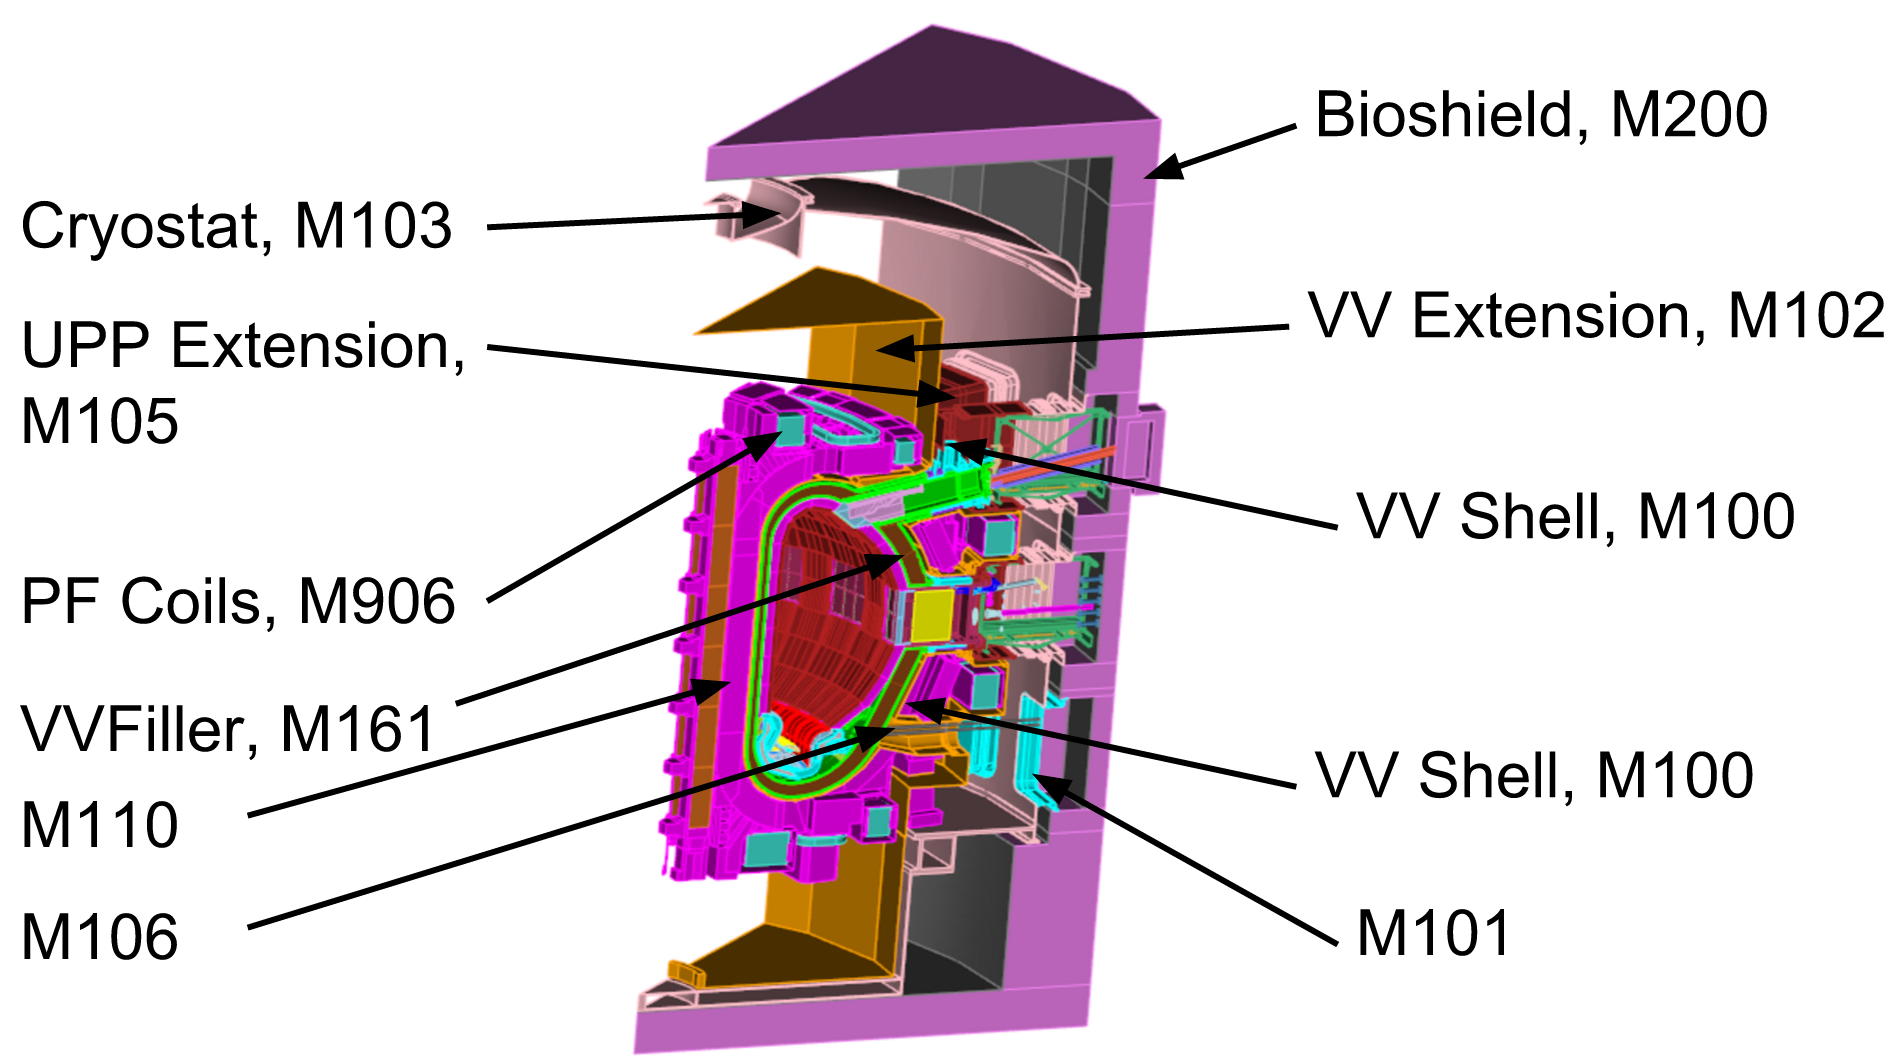
\includegraphics[scale=0.32]{../plots/cad/mats/label_1.png}
  \includegraphics[scale=0.32]{../plots/cad/mats/label_2.png}
  \caption{Section showing some of the major tokamak structural materials}
  \label{fig:material_assign_1}
\end{figure}

\begin{figure}[p]
  \centering
  \includegraphics[scale=0.32]{../plots/cad/mats/label_3.png}
  \caption{Materials found in the divertor region}
  \label{fig:material_assign_2}
\end{figure}

\begin{figure}[p]
  \centering
  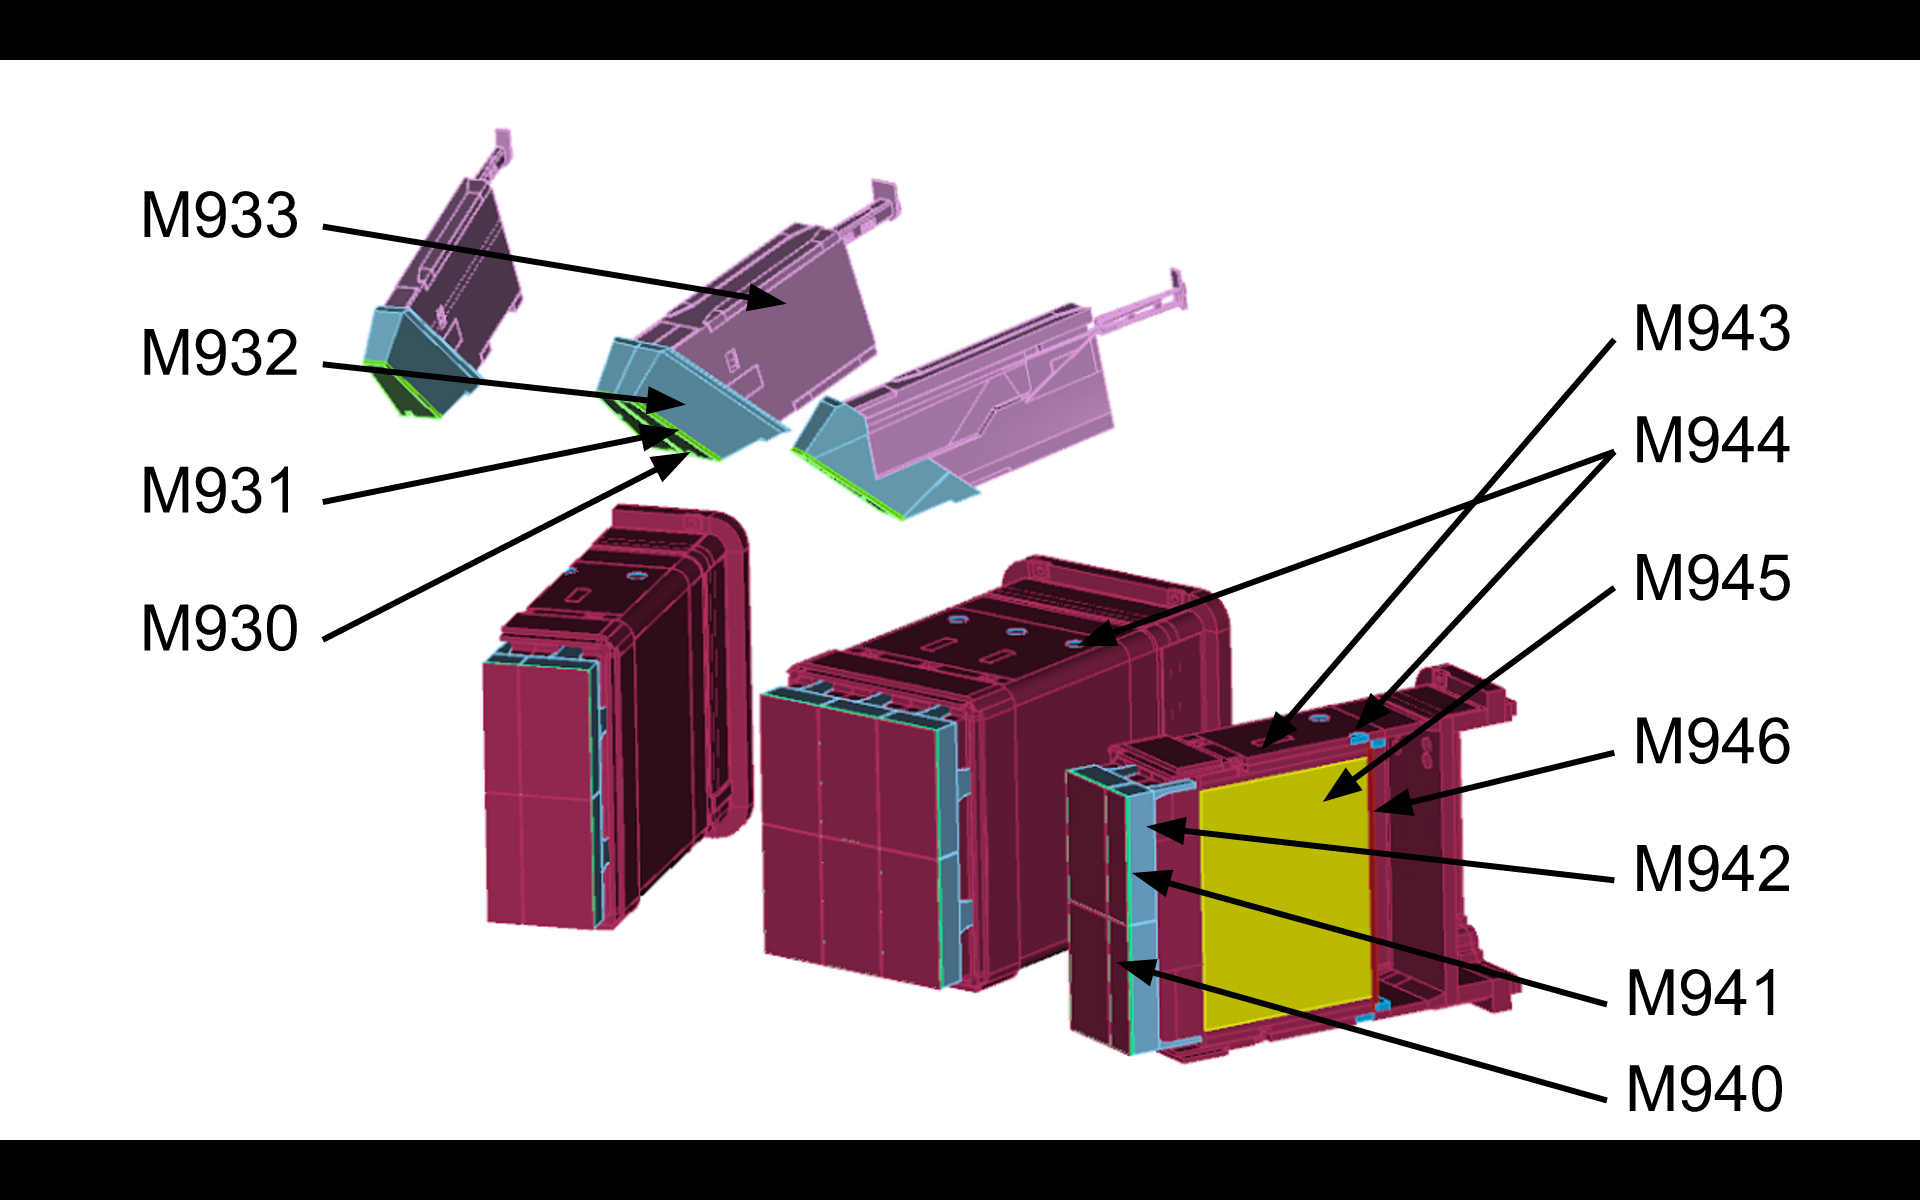
\includegraphics[scale=0.32]{../plots/cad/mats/label_4.png}
  \caption{Materials found in the upper and equatorial port plugs }
  \label{fig:material_assign_3}
\end{figure}

\begin{figure}[p]
  \centering
  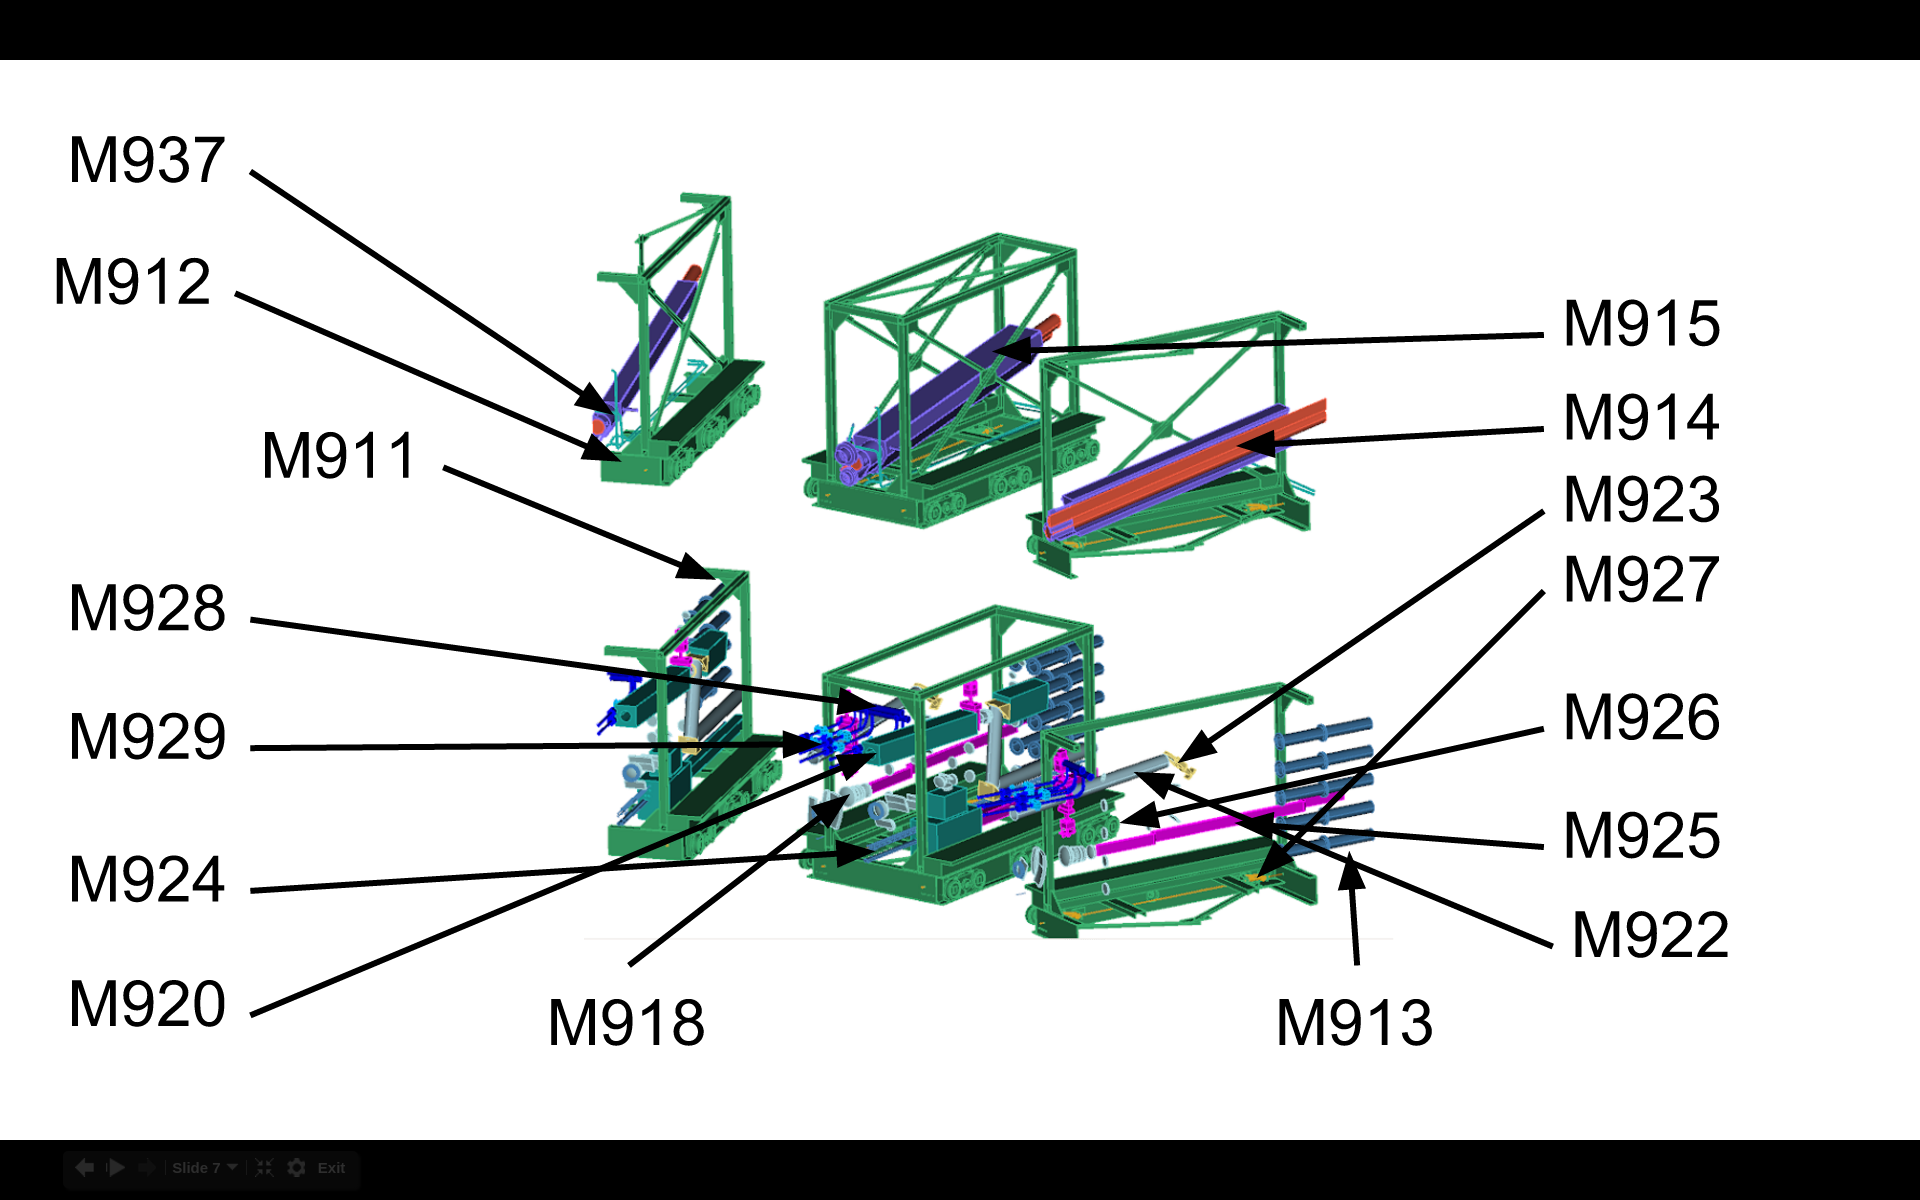
\includegraphics[scale=0.32]{../plots/cad/mats/label_5.png}
  \caption{Materials found in the equatorial and
           upper port interspace region}
  \label{fig:material_assign_4}
\end{figure}

\begin{figure}[p]
  \centering
  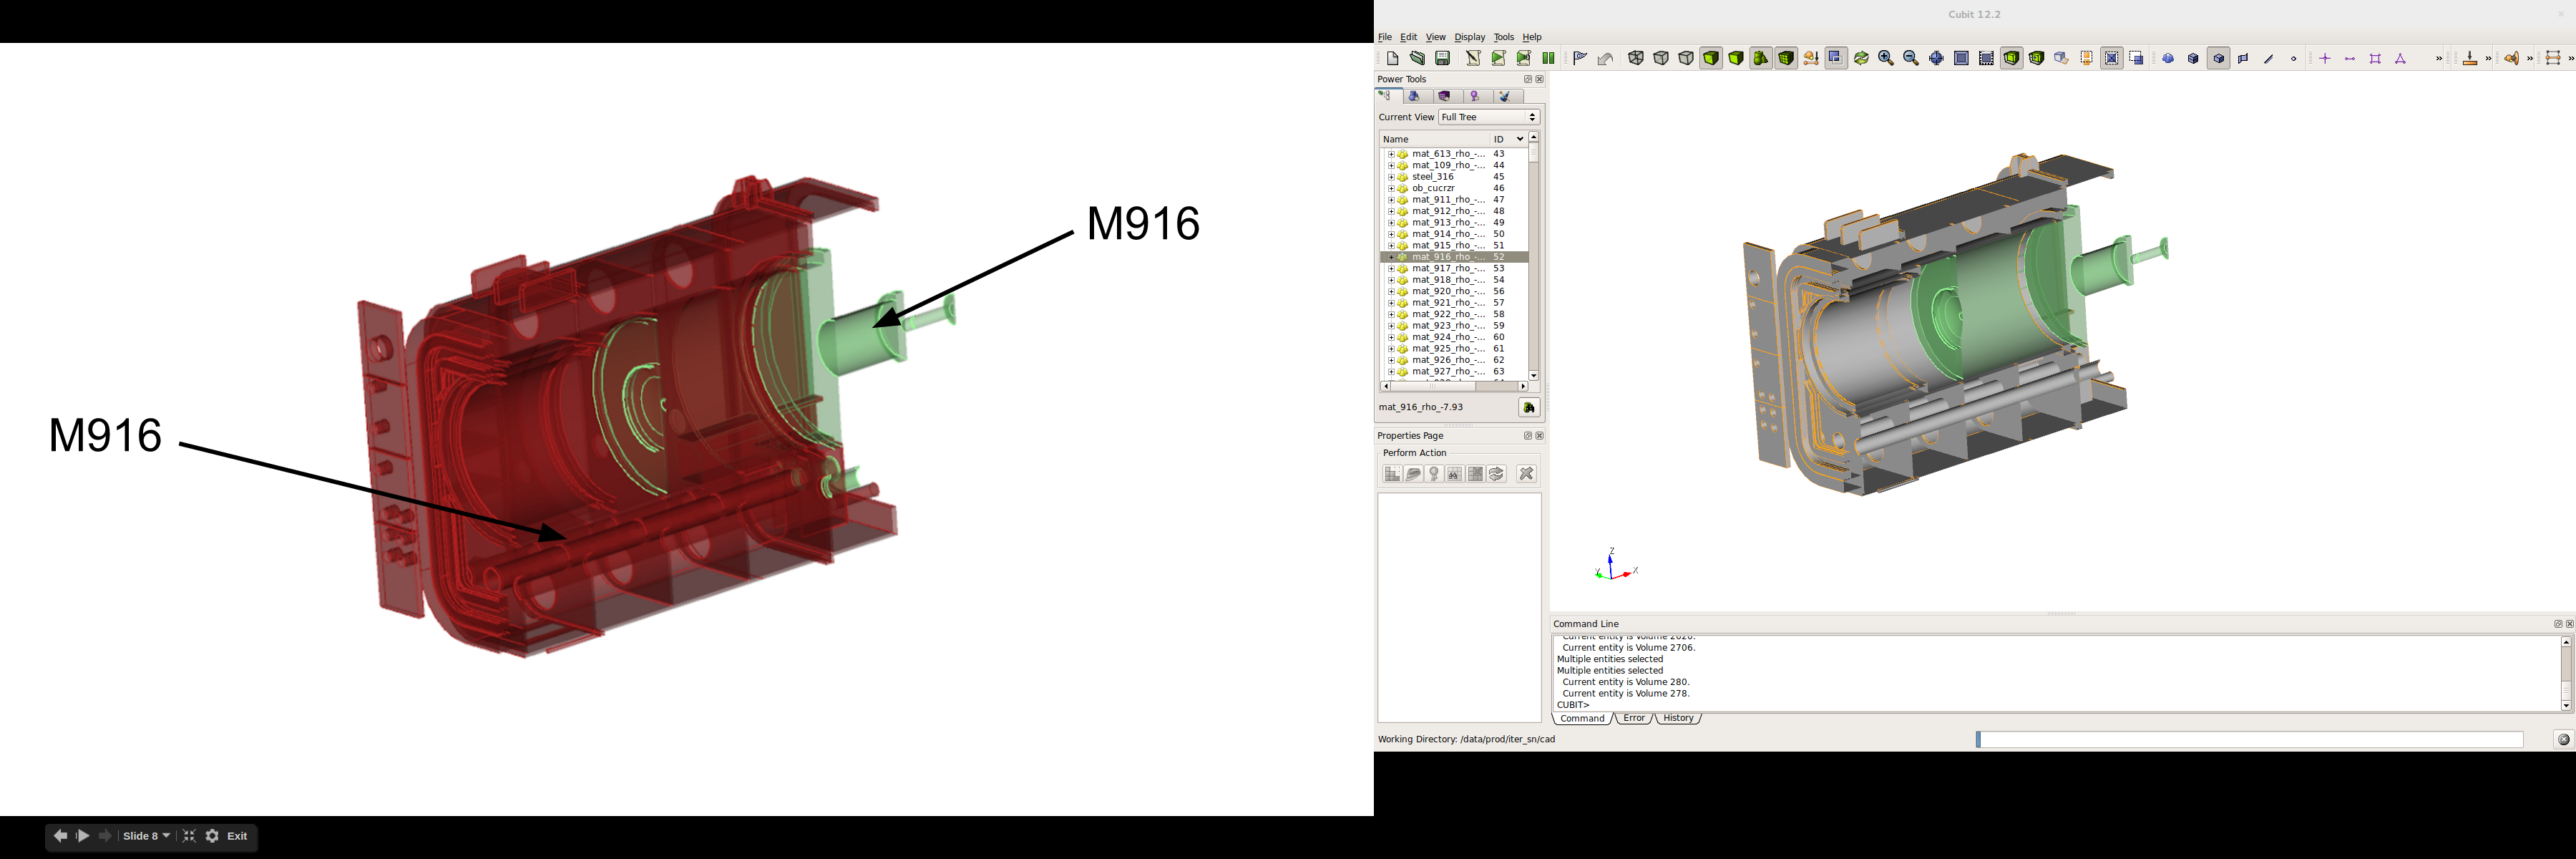
\includegraphics[scale=0.32]{../plots/cad/mats/label_6.png}
  \caption{Materials found in the Cryopump}
  \label{fig:material_assign_5}
\end{figure}

\newpage
\clearpage
\subsection{Software Programs \& Validation Status}
\subsubsection{DAGMC}
The \gls{dagmc} is a toolkit developed at the \gls{uw}
designed specifically for ray tracing efficiently on complex \gls{cad} based
geometries. The \gls{dagmc} toolkit is distributed as part of \gls{moab} and
is completely open source. Input to \gls{dagmc} is a \gls{moab} mesh file
which contains the faceted representation of the \gls{cad} geometry, this
is loaded and oriented bounding box (OBB) acceleration structures are built
to speed each ray fire query.

\subsubsection{DAG-MCNP5}
As \gls{dagmc} only satisfies the ray-tracing 
and related queries for Monte Carlo transport, it is necessary to combine it
with a Monte Carlo physics code to provide the majority of radiation transport
capability. For this work, \gls{mcnp5} \cite{mcnp} was selected as that physics
code as it has been identified by ITER as the reference tool for Monte Carlo 
radiation transport.  DAG-MCNP5 \cite{dagmc} is a version of \gls{mcnp5} where the core ray
queries (point in volume, ray fire, next volume, etc) have their \gls{mcnp5}
versions replaced with the \gls{dagmc} equivalents. DAG-MCNP5 has been validated
\cite{dagmc_validation} and tested in several ITER analysis in the past.

\subsubsection{ADVANTG}
The \gls{advantg} software automates the 
process of generating variance reduction parameters for continuous-energy Monte 
Carlo simulations of fixed-source neutron, photon, and coupled neutron-photon 
transport problems using \gls{mcnp5} \cite{advantg}. \gls{advantg} generates 
space and  energy-dependent mesh-based weight-window bounds and biased source 
distributions using three-dimensional discrete ordinates solutions of the 
adjoint transport equation that are calculated by the Denovo package 
\cite{denovo}. 
\\
\\
\gls{advantg} implements the \gls{cadis} method \cite{wagnerNSECADIS} and the 
\gls{fwcadis} method \cite{wagnerNSEFWCADIS} for generating variance reduction 
parameters. The \gls{cadis} and \gls{fwcadis} methods provide a prescription for
generating space and energy-dependent weight-window targets and a consistent 
biased source distribution. The \gls{cadis} method was developed for accelerating
individual tallies, whereas \gls{fwcadis} was developed for multiple tallies and
mesh tallies. The \gls{cadis} method has been demonstrated to provide speed-ups 
in the tally \gls{fom} of $O(10^1-10^4)$ across a broad range of radiation 
detection and shielding problems. The \gls{fwcadis} method has been shown to produce
 relatively uniform statistical uncertainties across multiple cell tallies and 
large space- and energy-dependent mesh tallies in real-world applications.
\\
\\
\gls{advantg} was updated to support \gls{dagmc}-based calculations. This was 
accomplished by linking the \gls{advantg} mapping functions that are used to 
map the Monte Carlo geometry onto the Denovo mesh to the \gls{dagmc}
ray-tracing routines \cite{biondoMC2015}. With this new capability, 
\gls{advantg} was able to map the geometry of the Clite \gls{cad} model onto a 
Cartesean mesh to use Denovo to generate the variance reduction parameters 
for the DAG-MCNP5 calculations of the neutron fluxes.

\subsubsection{PyNE}
The \gls{pyne} \cite{Scopatz2012b} project aims to
make a Python-accessible library of well validated and tested
Python and C++ functions and capabilities available to nuclear engineers 
across the world.
For this project we used the following capabilities of \gls{pyne}.
\begin{itemize}
  \item{the \texttt{pyne.mesh} class to combine meshes, with an appropriate
        combined statistical error}
  \item{the \texttt{pyne.r2s} class to produce \gls{r2s} inputs and outputs}
  \item{the \texttt{pyne.alara} class to produce \gls{alara_c} inputs}
  \item{the \texttt{pyne.mcnp} class to read \gls{mcnp5} meshtal files}
  \item{the \texttt{pyne.source\_sampling} capability to enable sampling of 
        mesh-based multi-group sources in \gls{mcnp5} }
\end{itemize}
The \gls{pyne} capabilities are interoperable with \gls{dagmc} output and handles
most post-process operations in the analysis.

The \texttt{pyne.source\_sampling} capability is a series of functions based on
the user-customization source routine of \gls{mcnp5}, but designed for sampling
the source characteristics from a very large mesh-based multi-group source.  In
these circumstances, the source position and energy are distributed over millions
of histogram bins requiring specialized methods for efficient sampling.  The
\texttt{pyne.source\_sampling} capability can be configured to implement analog
sampling, i.e. selection a space-energy mesh voxel directly according to its
relative emission intensity, or to implement uniform sampling, i.e. selecting the
spatial voxel uniformly in space and adjusting the particle weight accordingly.
The latter approach is important when the relative source intensity varies by
many orders of magnitude across the geometric extents of the problem, as in 
this problem.

Another important feature of the \texttt{pyne.source\_sampling} capability is
void rejection.  Since many of the activation voxels may contain a combination
of solid material and vacuum, it is important that photon are only born in the
non-void spaces.  Allowing photons to be born in the void spaces would ignore
important self-shielding effects in the source in those cases.  Therefore,
once a spatial voxel is selected, the location within that voxel is chosen
uniformly in space and tested to ensure that this location is in a non-void
space.  If it is found to be in a void space, then another location is sampled
uniformly.  Since some voxels could theoretically contain very small fractions
of non-void space, calculation efficiency requires a limit on the number of
times a particular voxel is resampled before selecting a new voxel. This is
exacerbated by uniform mesh sampling since voxels may be selected for sampling
even if the total source strength is low, possibly due to a very small
non-void volume.

\subsubsection{ALARA}
\gls{alara_c} \cite{alara} is a nuclear inventory code developed at the \gls{uw}
The unique feature of \gls{alara_c} is the way it handles the
pathways of the reactions, all of the potential pathways are accounted for and
duplicate links linearised. \gls{alara_c} is used in this analysis as the method
of producing gamma ray sources for \gls{r2s} shutdown photon calculations.

\subsection{Validation Status}
\subsubsection*{Analysis Codes}
The analsysis codes used in these calculations are shown in Table 
\ref{table:validation}. These codes were used to directly produce results shown
in this report.
\begin{centering}
 \begin{table}[ht!]
  \begin{tabular}{c | c | c | c}
  \hline
  Code & Version & Validation Status & References \\
  \hline 
  DAG-MCNP5 & 1.0 & Production & \cite{dagmc_validation}\\
  \gls{alara_c} & 2.9.1 & Production & \cite{alara}\\
  \gls{advantg} & 3.0.2 & Production & \cite{advantg}\\
  Denovo & 5.3 & Production & \cite{denovo} \\
  \end{tabular}
 \caption{List of Analysis codes used and their validation status}
 \label{table:validation}
 \end{table}
\end{centering}

\subsubsection*{Auxilliary Codes}
The auxiallary codes used in the this report are shown in Table 
\ref{table:validation_aux}. These codes were not directly used to 
produce results, but were used to either process or produce input
and output data.
\begin{centering}
 \begin{table}[ht!]
  \begin{tabular}{c | c | c}
  \hline
  Code & Validation Status & References \\    
  \hline
  pyne.mesh & Validated by unit tests & - \\
  pyne.r2s & Validated & \cite{pyne_r2s} \\
  pyne.alara & Validated & \cite{pyne_r2s} \\
  pyne.mcnp & Validated & \cite{pyne_r2s} \\
  pyne.source\_sampling & Validated & \cite{pyne_r2s} \\
  yt 3.2 & Validated by unit tests & n/a \\
%% NOTE [PPHW] do all codes need validation?
 \end{tabular}
 \caption{List of auxilliary codes and their validation status}
 \label{table:validation_aux}
 \end{table}
\end{centering}

\newpage
\subsection{Solution Methodology}
\label{section:method}
\subsubsection{Neutron Transport}
The neutron transport calculations were performed using version 1.0 of DAG-MCNP5.
This version is derived from the RSICC source code version 1.60 of \gls{mcnp5}
with modifications for \gls{dagmc} applied, as represented in commit \texttt{e12e2a3}
of the \gls{uw} source code repository for DAG-MCNP5.
The two batches of calculations were performed, one
case with the B$_4$C liner and one without.  
In each case, the neutron flux was tallied in 175 energy groups using the
VITAMIN-J structure \cite{vitaminj} as shown in Appendix B \ref{appendix_b}.

%% NOTE [PPHW]: is vitamin=j correct here?

\subsubsection{Mesh Domain Decomposition}
The level of detail present in the faceted geometry files impacts the amount of
memory required to run the calculation, this combined with the large and
detailed weight window file and the need for 175 energy group neutron spectra
in each voxel means that the calculation requires significant memory resources,
in excess of 12 Gb per process.  %% 12 Gb after splitting into 7 meshes, or before?
To mitigate these memory requirements, the calculation was split into seven 
calculation domains, shown in Figure
\ref{fig:mesh_domains}, which bound the regions of the problem requiring
activation. In addition to reducing the memory requirements for each calculation
simply due to the decomposition of the tally domain, dividing the mesh tally 
domains in this manner reduces the number of neutron mesh voxels that are 
outside the boundary of the 40$^{\circ}$ sector, further reducing the overall memory
requirements.

\begin{figure}[ht!]
  \centering
  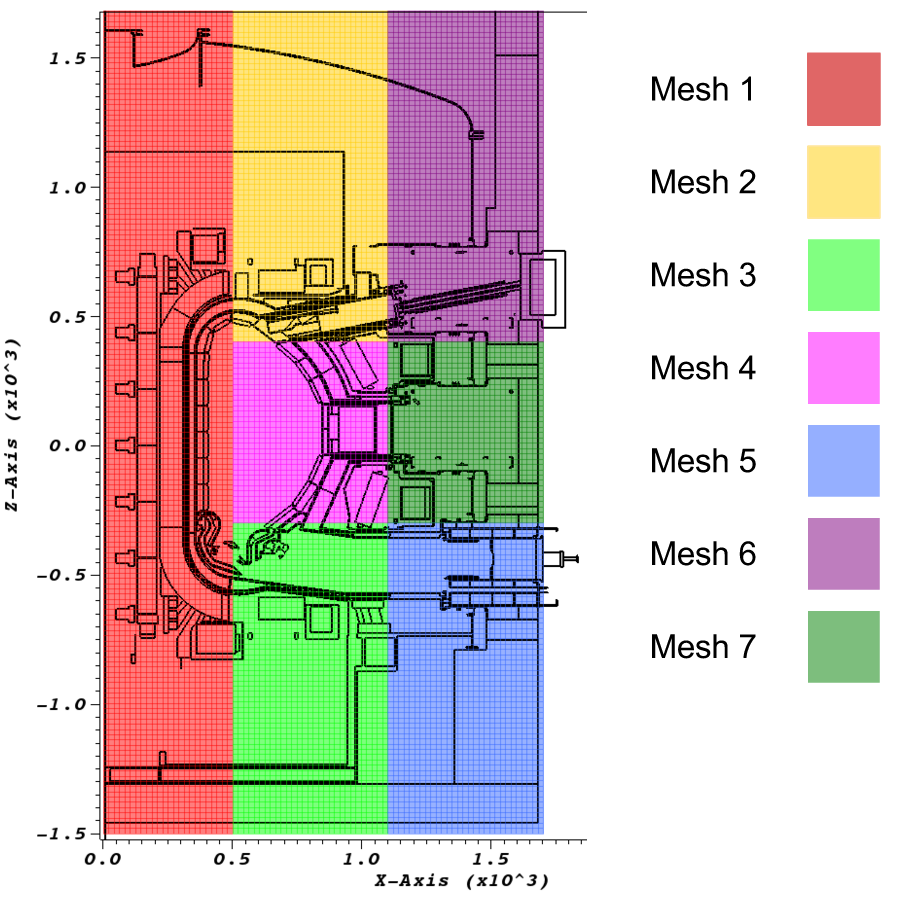
\includegraphics[scale=0.4]{../plots/transport/job_splits.png}
  \caption{The seven different mesh domains, (left) shown with some transparency
           to indicate where the major boundaries end and (right) showing the
           absolute scale of the mesh elements}
  \label{fig:mesh_domains}
\end{figure}

The physical size and boundaries that were used in the calculation
can be found in Table \ref{table:mesh_sizes}. With \gls{r2s} calculations there 
is a subtle interplay between the size of the mesh elements and the number of mesh
elements; the larger the mesh elements the lower the statistical errors will be
for a given fixed number of particles but the mesh will conform poorly to the
geometry, and vice versa. In this calculation the maximum number of mesh
elements in a given mesh is dictated by the size that the given mesh will
occupy in memory when transferred to an \gls{alara_c} geometry. 

\begin{centering}
 \begin{table}[ht!]
  \begin{tabular}{c | c | c | c | c}
  \hline 
  Mesh & Dimension & Start position (cm) & End position (cm) & Number of bins\\
  \hline 
  \multirow{3}{*}{Mesh 1} & X & 0.0 & 500.0 & 25 \\ & Y & -250.0 & -250.0 & 25 \\
  & Z & -1500.0 & 1900.0 & 170 \\
  \hline
  \multirow{3}{*}{Mesh 2} & X & 500.0 & 1100.0 & 30 \\ & Y & -500.0 & 500.0 & 50\\
  & Z & 400.0 & 1900.0 & 75 \\
  \hline
  \multirow{3}{*}{Mesh 3} & X & 500.0 & 1100.0 & 30 \\ & Y & -500.0 & 500.0 & 50 \\
  & Z & -1500.0 & -300.0 & 60 \\
  \hline
  \multirow{3}{*}{Mesh 4} & X & 500.0 & 1100.0 & 30 \\ & Y & -500.0 & 500.0 & 50 \\
  & Z & -300.0 & 400.0 & 35 \\
  \hline
  \multirow{3}{*}{Mesh 5} & X & 1100.0 & 1700.0 & 30 \\ & Y & -600.0 & 600.0 & 60 \\
  & Z & -1500.0 & -300.0 & 60 \\
  \hline
  \multirow{3}{*}{Mesh 6} & X & 1100.0 & 1700.0 & 60 \\ & Y & -600.0 & 600.0 & 60 \\
  & Z & 400.0 & 1900.0 & 75\\
  \hline
  \multirow{3}{*}{Mesh 7} & X & 1100.0 & 1700.0 & 30 \\ & Y & -600.0 & 600.0 & 60 \\
  & Z & -300.0 & 400.0 & 36 
  \end{tabular}
 \caption{The meshes used in the problem, their start and end coordinate and
          number of divisions}
 \label{table:mesh_sizes}
 \end{table}
\end{centering}

\subsubsection{Variance Reduction}
The weight window parameters were generated using the \gls{ornl} code
\gls{advantg}, specifically using DAG-\gls{advantg}, which allows a
\gls{dagmc} geometry to be read and the geometry and material data handed off to
Denovo. The weight windows were produced using the \gls{fwcadis},
which attempts to produce a weight window map which tries to get particles
everywhere in the model, as opposed to \gls{cadis} for example, which
attempts to get results to a small number of specific regions.  Since no 
fully validated methodologies yet exist to determine the most important regions of
neutron phase space for a \gls{sdr} calculation, this problem used a \gls{fwcadis}
configured to achieve uniform statistical variance throughout the neutron mesh
tally regions.  One consequence of this configuration is that computational
effort may be expended to increase the neutron population in unimportant regions 
of neutron phase space.

\gls{advantg} only implements reflecting boundaries on the principal axes of a 
problem, requiring a geometry that fills either a 90$^{\circ}$ or 180$^{\circ}$ 
sector, or fills the entire 360$^{\circ}$.

%% NOTE [PPHW]: Need to confirm with AMI exactly how he configured the
%%  fw-cadis including: the number of energy groups and spatial mesh (I
%%  think/assume this is the same as the neutron tally mesh?)

\subsubsection{Job-level Parallelism}
Parallelism over many processors was necessary to achieve this calculation in
a reasonable time. Methodologies with extreme variance reduction can produce
pathologically long histories.  In such problems, individual histories may
experience the variance reduction scheme in a way that results in millions of
splitting events.  Such rare histories can overwhelm the total computer time
needed for a simulation appearing to never actually reach completion, with
severe negative impacts on load balancing under a typical message passing
(MPI) parallel approach.  In the worst cases, the entire MPI job never reaches
completion yielding no results.  In the job parallel approach, instead of
distributing packets of independent histories from within a single simulation,
a batch of independent jobs are launched each with the same packets of
independent histories.  While it is still possible for some of these jobs to
not reach completion, this approach is amenable to submitting a surplus of
jobs and using a subset of these statistically independent jobs to produce the
final results.  In both cases, independent histories are guaranteed by
selecting the number of histories and the first history for each process to
avoid overlap.  

%% NOTE [PPHW]: Should integrate this discussion (previously in the Conclusion
%% section) with the above.  Maybe it's all covered now above and we just delete?
%% But some questions: 
%%
%% *) Does this mean to say that we suggest using all 3 concepts, or just some
%%    subset. It seems to make more sense as the latter to me!  If the latter
%%    which do we do?  and why all the suggestions - just document what we do.
%% *) Did we use CTME or NPS for the HTC calcs?It must have been NPS to avoid
%%    overlapping histories.

When variance reduction parameters that span over
 many orders of magnitude are being used in non-analog Monte Carlo simulations,
 it is difficult to estimate the computational time needed to simulate each 
particle because some of these particles undergo millions of splitting events. 
To overcome this problem, the authors suggest 1) using the computer time cutoff
 (CTME) card in MCNP to stop the MCNP runs after reaching a certain amount of 
running time without losing the results, 2) to increase the frequency of the 
printing and dumping of MCNP using the PRDMP card, 3) and to avoid the use of 
the MPI version of MCNP. The Monte Carlo calculations can still run in parallel
 without using MPI by submitting independent jobs with different random number 
seeds and statistically averaging the results as demonstrated in this report. 
The load balancing of the MPI  version of MCNP does not consider the huge 
differences in the computational times needed to simulate different histories
 that are typical with the use of variance reduction parameters that span many 
orders of magnitude. The MCNP runs will not be stopped even if the computational
 time exceeded the time of the  CTME card until MCNP reaches the printing and 
dumping stage. Without increasing the frequency of these dumping events, the 
time of the CTME card may be ignored for a very long time.

The combination of mesh domain decomposion and job parallelism is shown in
Figure \ref{fig:mesh_splitting}.  
The spatial domain of the problem is duplicated and a given
mesh tally superimposed onto the geometry. Several single core simulations are
launched for that specific meshtally but the random number seed is strided in
such a way that no process will share the same histories with another job.  
This is performed using the \texttt{rand hist=n} command in \gls{mcnp5}.

\begin{figure}[ht!]
  \centering
  \includegraphics[scale=0.3]{../plots/method/neutron_method.png}
  \caption{The high throughput methodology, splitting a given MCNP calculation
           into smaller calculations spanning a contiguous random number seed
           space}
  \label{fig:mesh_splitting}
\end{figure}


%% NOTE [PPHW]: We never say how many histories we used, whether total or in
%% each individual job.  We should somewhere indicate the total number of
%% histories for each mesh and how many individual jobs were used (not how
%% many were launched - or maybe?).
%%
%% I see this comes in a later section on Calculation Details...  is this 
%% based on the outline from ORNL?  It seems odd to put it so late.

\subsubsection{Activation}
The activation calculations are performed using the spatially dependent neutron
spectra determined in the previous step. The activation calculations proceed as
a set of standard mesh based \gls{r2s} calculations typically proceed since the 
meshes do not overlap, this is shown schematically in Figure
\ref{fig:activation_method}
\begin{figure}[ht!]
  \centering
  \includegraphics[scale=0.3]{../plots/method/activation_method.png}
  \caption{The methodology of having several activation meshes distributed
           across a given problem to generate several spatially discrete
           decay sources}
  \label{fig:activation_method}
\end{figure}
The geometry under each voxel in the mesh is queried to 
determine the average material composition by volume fraction, a material 
description is developed and recorded for running in an inventory code. In the 
case of \texttt{pyne.r2s} a full \gls{alara_c} input deck is produced which can
then be executed and the final shutdown photon sources produced. From a single
inventory calculation the decay photon sources for all the subsequent decay
times can be generated.  The photon sources were each generated using 24 photon
energy groups using the FISPACT 24 group structure.

\begin{table}[ht!]
   \begin{tabular}{| l | c | c |}
      \hline
      Energy Group Number & Lower Energy Bound & Upper Energy Bound \\
      \hline
      0 & 0.0 & 10.0 \\
      1 & 10.0 & 20.0 \\
      2 & 20.0 & 50.0 \\
      3 & 50.0 & 100.0 \\
      4 & 100.0 & 200.0 \\
      5 & 200.0 & 300.0 \\
      6 & 300.0 & 400.0 \\
      7 & 400.0 & 600.0 \\
      8 & 600.0 & 800.0 \\
      9 & 800.0 & 1000.0 \\
      10 & 1000.0 & 1220.0 \\
      11 & 1220.0 & 1440.0 \\
      12 & 1440.0 & 1660.0 \\
      13 & 1660.0 & 2000.0 \\
      14 & 2000.0 & 2500.0 \\
      15 & 2500.0 & 3000.0 \\
      16 & 3000.0 & 4000.0 \\
      17 & 4000.0 & 5000.0 \\
      18 & 5000.0 & 6500.0 \\
      19 & 6500.0 & 8000.0 \\  
      20 & 8000.0 & 10000.0 \\
      21 & 10000.0 & 12000.0 \\
      22 & 12000.0 & 14000.0 \\
      23 & 14000.0 & 20000.0 \\  
      \hline
\end{tabular}
\caption{The photon group boundaries used in this analysis}
\label{tab:photon_boundaries}
\end{table}


\subsubsection{Photon Transport}
The photon transport proceeds using the same computational model as in the
neutron calculation, but without variance reduction and with a mesh-based
photon source and appropriate normalisation as determined using the activation
step.  The photon dose is tallied using ICRP-74 flux-to-dose conversion
factors.  Because the photon dose is tallied in a single bin over all
energies, tally mesh decomposition is not necessary for photon transport.  The
dose response from each of the seven source mesh is simulated over the entire
domain for each of the decay times.  The total dose is found by superposition
by simply adding the full domain's results from each source mesh, and
combining estimates of the statistical error appropriately.
\\
\\

With two cases, seven source meshes and three decay times, this led to 42
independent photon transport calculations, each with $10^8$ histories sampled
using the \texttt{pyne.source\_sampling} routines configured for uniform
sampling and void rejection of 0.01.  The dose response mesh tallies in each
problem were normalised using the appropriate total source intensity as determined
by the appropriate inventory calculation.

\subsection{Software Risk Assessment}
All software used for analysis is current, validated and verified. DAG-MCNP5
is validated using an extensive test suite which checked every two weeks against
the current state of a number of software libraries.  The \gls{dagmc} interface
istelf is controlled under continuous integration; a complete set of unit and
regression tests are performed each time a developer proposes a change to the
software.  \gls{dagmc} itself depends upon MOAB, which also operates under a
similar continuous integration strategy.
\\
\\
\gls{pyne} is also maintained under a continuous integration strategy.  
Formal verification for indvidual parts of \gls{pyne} are performed on an as
needed basis, for example with \texttt{pyne.r2s} on the FNG shutdown dose rate
experiment. \cite{biondoFED2016}
\\
\\
The plotting tool yt, is a tool that originates from the astrophysics community used
for plotting very large datasets. Like the other tools mentioned here, yt is no different
in software development practises, version control, code reviews and unit testing are
used extensively. There are several features that make yt an attractive 
tool for plotting, as opposed to the more commonly encountered Visit from LLNL, specifically
its capability to read native MOAB meshes, the speed at which it slices stl overlays and 
its convenient scripting capabilities lead to its use in this report.
\\
\\
The Denovo discrete ordinates solver is built against a set of verifcation 
problems and unit tests. It is distributed as part of the SCALE code system, which imposes
a quality control plan found in \cite{scale_qa}. In this analysis Denovo was exclusively
used by \gls{ornl} as part of \gls{advantg} to produce weight windows for this analysis.

\clearpage
\newpage
\section{Inputs, Assumptions and Engineering Judgements}

\subsection{Neutron Source}
As used in typical ITER analysis the reference ITER neutron source 
\cite{iter_n_src} with
reflecting boundary conditions is assumed to adequately represent the
%% NOTE [PPHW]: Is this really an assumption?  No need to draw attention 
%%              to this as an assumption - it's the standard!
true 360$^{\circ}$ neutron source. The ITER supplied \gls{mcnp5} SDEF was used
completely unmodified. The on-load neutron data is normalised as part of the 
\gls{r2s} calculation to correspond to the 
average power for the pulse being modelled. However for reference,
the highest power used in the activation calculation was 500 MW, which is
equivalent to $1.98 \times 10^{18}$ neutrons per second in the 40$^{\circ}$
sector. Given that this is the IO approved neutron source description, it is
assumed to be adequate for this simulation.  Neutrons from activated water
were not considered in this problem as they represent a negligible addition
to the fluence of neutrons from the fusion source.

\subsection{Irradiation Scenario}
The irradiation scenario used in this work was the SA-2 \cite{sa2_irradiation}, 
shown in Table \ref{tab:irrad_scenario}. Relative strength refers to the 
neutron source normalisation used relative to nominal 500 MW operations.

\begin{table}[ht!]
   \begin{tabular}{| l | c | c | c |}
      \hline 
      Irradiation Period & Neutron Power (MW) & Source Normalisation (n/s) &  Relative Strength \\
      \hline
      2 Years & 2.7 & $1.061\times10^{17}$ & 0.0053 \\
      10 Years & 20.6 & $8.517\times10^{17}$ & 0.0412 \\
      1.325 Years & 41.5 & $1.643\times10^{18}$ & 0.0830 \\
      \cellcolor{blue!25} \cellcolor{blue!25} 400 Seconds & \cellcolor{blue!25} 500.0 & $1.980\times10^{19}$ & \cellcolor{blue!25} 1.0  \\
      \cellcolor{blue!25} 3920 Seconds & \cellcolor{blue!25} 0.0 & \cellcolor{blue!25} 0.0 & \cellcolor{blue!25} 0.0 \\
      \cellcolor{green!25} 400 Seconds & \cellcolor{green!25} 700.0 & \cellcolor{green!25} $2.772\times10^{19}$ &\cellcolor{green!25} 1.4 \\
      \cellcolor{green!25} 3920 Seconds & \cellcolor{green!25} 0.0 & \cellcolor{green!25} 0.0 &\cellcolor{green!25} 0.0 \\
      \hline
\end{tabular}
\caption{The table shows the SA-2 scenario for irradiation, note the
         cells in \textcolor{blue!25}{blue} are repeated 17 times
         and the cells in \textcolor{green!25}{green} are repeated 3
         times.}
\label{tab:irrad_scenario}
\end{table}
In this report time periods following machine shutdown are of interest,
$10^5$ s, $10^6$ s and $10^7$ s, approximately corresponding to 27 
hours, 14 days, and 116 days post shutdown respectively.

\subsection{Geometry}
The geometry used in this simulation was collected from a number of sources;
some models were generated directly from CAD drawings supplied by the
drawing office of US ITER and the IO, some were intermediate CAD files produced
as part of other simulations, and some were generated by \gls{uw} to meet a
perceived deficiency in the file. Irrespective of this, the \gls{dagmc} method
allows the exact representation of the underlying CAD to be used without
approximation.
%% NOTE [PPHW]: What does "perceived deficiency in the file" mean?
\\
\\
The geometry is defined starting at the centre column (x = 0.0 cm) and ends
beyond the bioshield (x = 1800 cm), truncation of details relative to the full
ITER device CAD model begins on the port cell side of the bioshield plugs,
results beyond the bioshield should therefore be not be used for any
analysis purposes.  It is assumed that the 40$^{\circ}$ sector of the geometry
is sufficiently representative and reflecting boundaries were applied on the
planes at each side of the sector.

\subsection{Materials and Nuclear Data}
\subsubsection{Materials}
The full description of material contents can be found in the Appendix. The 
origin of each material is described in Table \ref{tab:material_origin}. 

\begin{centering}
 \begin{longtable}[ht!]{ p{0.2\textwidth} | p{0.3\textwidth} | p{0.3\textwidth} }
  \hline 
  Material Number & Description & Origin \\
  \hline
  M29  & Copper &  CLITE V1 \\
  M74  & Tungsten &  CLITE V1 \\
  M100  & 316L(N)-IG &  CLITE V1 \\
  M101  & &  CLITE V1 \\
  M102  & &  CLITE V1 \\
  M103  & &  CLITE V1 \\
  M104  & &  CLITE V1 \\
  M105  & &  CLITE V1 \\
  M106  & &  CLITE V1 \\
  M107  & &  CLITE V1 \\
  M108  & &  CLITE V1 \\
  M109  & &  CLITE V1 \\
  M110  & &  CLITE V1 \\
  M111  & &  CLITE V1 \\
  M162  & &  CLITE V1 \\
  M170  & &  CLITE V1 \\
  M200  & &  CLITE V1 \\
  M303  & &  CLITE V1 \\
  M400  & &  CLITE V1 \\
  M601  & &  CLITE V1 \\
  M602  & &  CLITE V1 \\
  M603  & &  CLITE V1 \\
  M611  & &  CLITE V1 \\
  M613  & &  CLITE V1 \\
  M621  & &  CLITE V1 \\
  M622  & &  CLITE V1 \\
  M623  & &  CLITE V1 \\
  M631  & &  CLITE V1 \\
  M906  & &  CLITE V1 \\
  M907  & &  CLITE V1 \\
  M908  & &  CLITE V1 \\
  M910 & B$_4$C & Bespoke  \\
  M911 & Al T6061 & Bespoke  \\
  M912 & Al T6061 & Bespoke  \\
  M913 & Copy M100 & CLITE V1\\
  M914 & Copy M100 & CLITE V1\\
  M915 & Copy M910 & Bespoke \\
  M916 & Copy M100 & CLITE V1\\
  M917 & Cryopipes & \cite{cryopump_communication}\\
  M918 & Copy M100 & CLITE V1 \\
  M920 & Copy M100 & CLITE V1 \\
  M921 & Copy M100 & CLITE V1 \\
  M922 & Copy M100 & CLITE V1 \\
  M923 & Copy M100 & CLITE V1 \\
  M924 & Copy M100 & CLITE V1 \\
  M925 & Copy M100 & CLITE V1 \\
  M926 & Copy M100 - Frame Wheels & \cite{bertalot_communication}\\
  M927 & Copy M100 - Frame Wheels Drive & \cite{bertalot_communication}\\
  M928 & Copy M100 - Port Plug Frame & \cite{bertalot_communication}\\
  M929 & Copy M100 - Port Plug Pipes & \cite{bertalot_communication}\\
  M930 & Copy M100 & \cite{cryopump_communication}\\
  M931 & M100:0.7 M400:0.3 & \cite{bertalot_communication}\\
  M932 & M100:0.9 M400:0.1 & \cite{bertalot_communication}\\
  M933 & M100:0.9 M400:0.1 & \cite{bertalot_communication}\\
  M934 & M100:0.97 M400:0.03 & \cite{bertalot_communication}\\
  M937 & Copy M100 & \cite{cryopump_communication}\\
  M938 & Copy M100 & \cite{cryopump_communication}\\
  M939 & Copy M100 & \cite{cryopump_communication}\\
  M935 & First Wall & BL-lite \\
  M936 & First Wall & BL-lite \\
  M940 & Copy M100 & Diagnostics MCNP Model \\
  M941 & Copy M100 & Diagnostics MCNP Model \\
  M942 & Copy M100 & Diagnostics MCNP Model \\
  M943 & Copy M100 & Diagnostics MCNP Model \\
  M944 & EPP Drawers & Diagnostics MCNP Model \\
  M945 & EPP Contents & Diagnostics MCNP Model \\
  M946 & EPP Chunks & Diagnostics MCNP Model \\
 \caption{Table showing the origin of the material descriptions used}
 \label{tab:material_origin}
 \end{longtable}
\end{centering}

\subsubsection*{Nuclear Data}
Neutron Data - The neutron transport data used was \gls{fendl}-2.1/MC, as 
recommended by \gls{io} for ITER analysis. 
\\
\\
Activation Data - The activation data used was \gls{fendl}-3.0/A.
\\
\\
Photon Data - The standard photon data supplied with \gls{mcnp5} mcplib04 was 
used. This data ultimately falls back onto \gls{endf}/B-VI release 8 photo
atomic data.

\subsection{Transport Software}
The particle transport software used for this analysis was \gls{dag}-\gls{mcnp5}
which integrates the DAGMC toolkit into the Monte Carlo code \gls{mcnp5}. 
DAG-MCNP5 has been extensively used in other ITER analyses and has a significant
validation effort behind it. \gls{mcnp5} is the standard Monte Carlo transport code
used at ITER and therefore represents the predefined level of neutron and physics
required for this analysis.

These results also assume that results from a set of N independent Monte Carlo
simulations of M histories each, can be averaged to represent a single
simulation of N$\times$M histories.  It is further assumed that any N
simulations can be used, even if/when they do not represent a contiguous set
of histories, as long as they do not include any overlapping histories.

\subsection{Activation Software}
\gls{alara_c} is the \gls{uw}'s standard nuclear inventory code for performing
fusion relevant activation calculations. \gls{alara_c} has been validated against 
FISPACT \cite{fispact} in the past and gives numerically equivalent results. 

\newpage
\clearpage
\section{Neutron Transport Results and Conclusions}

\subsection{Calculation Details}
Using the methodology shown in Section \ref{section:method}, the neutron meshes
were split into 7 calculations. These jobs were submitted to the \gls{uw}
\gls{chtc} system in batches of 200 for each mesh, with seven meshes used to
determine the neutron flux, making a
total of 2800 individual \gls{mcnp5} simulations. These results were then
combined using \gls{pyne} to result in the statistically averaged final results.
Initially calculations were batched into groups of $5\times10^7$ particles per
batch, however these calculations did not finish in a timely enough manner and
were instead reduced to groups of $5\times10^6$ particles per batch. With the
smaller batching system calculations did finish, however, only 10\% of all
calculations for each mesh finished, but this represents $5\times10^7$ total
source histories for each mesh.
\\
\\
The individual meshtals were read using \gls{pyne}'s Mesh class and statistically
combined to produce the final result mesh for that region. In total fourteen 
condensed meshes were produced for this analysis, seven for the baseline case
and seven for the with B$_4$C liner. These condensed neutron mesh tallies were
then used for the subsequent activation calculations.

\subsection{Variance Reduction}
The weight windows generated by \gls{advantg} for this problem are shown in Figure
\ref{fig:wwinp}. 

\begin{figure}[ht!]
  \centering
  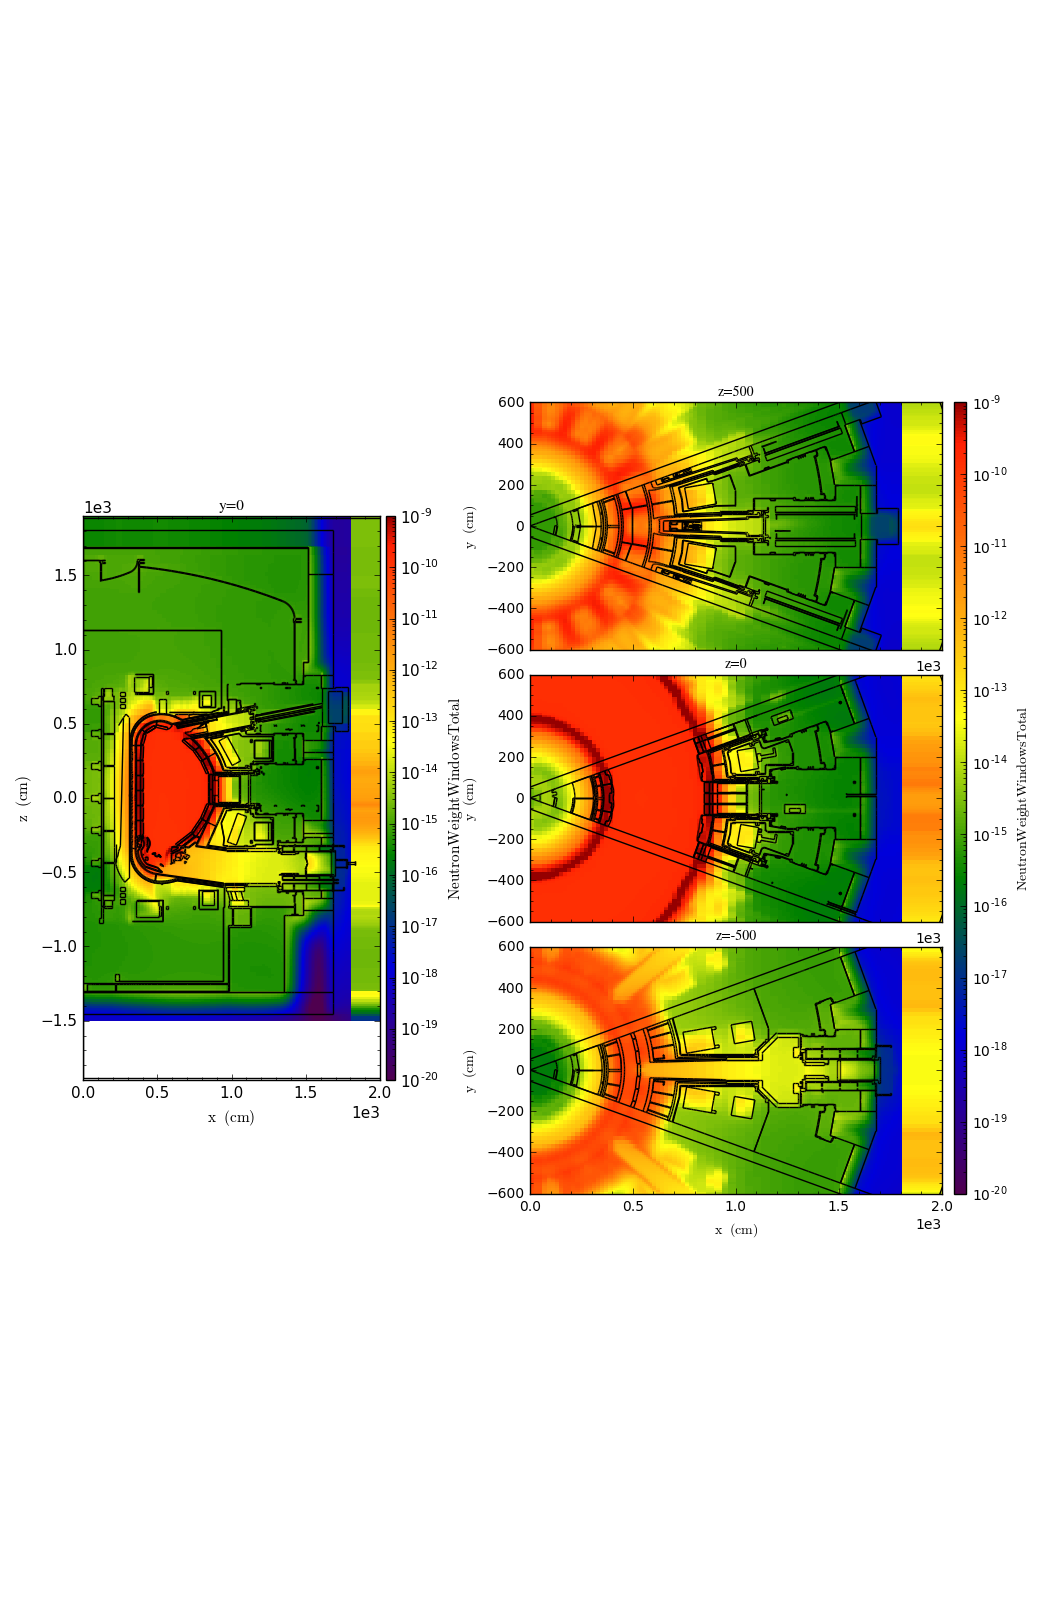
\includegraphics[trim={0cm 9cm 0cm 10cm},clip,scale=0.75]{../plots/wwinp/Neutron_Weight_Windows.png}
  \caption{Figure showing the ADVANTG produced neutron weight windows for y = 0.0 cm,
  z = 500.0 cm, z = 0.0 cm and z = -500.0 cm}
  \label{fig:wwinp}
\end{figure}

%% NOTE [PPHW]: which energy group is this WW data?

Several artifacts are worthy of note.  Despite being a deterministic code, Denovo
has handled the streaming of neutrons along the divertor duct well as shown in
left hand image of Figure \ref{fig:wwinp}. The overall span of the weight window
is seven orders of magnitude, which is largely proportional to the neutron
attenuation from the plasma to the port interspace, previous calculations put
the attenuation in the range of 6 to 8 orders of magnitude. There is some
evidence of component shadowing in the weight window solution in the right hand image
of Figure \ref{fig:wwinp} due to the neutron attenuation of some \gls{epi}
shielding around the diagnostic equipment. Overall the solution appears 
otherwise reasonable.
\\
\\
Since neither 90$^{\circ}$ nor 180$^{\circ}$ are integer multiples of 40$^{\circ}$,
this model must be rotated and replicated to fill a full 360$^{\circ}$ space.
\gls{ornl} specifically developed the 360$^{\circ}$
rotation feature for DAG-\gls{advantg} that allows rotationally symmetric
bodies.  Therefore, weight window values are observed beyond the 40$^{\circ}$ sector.

\subsection{Baseline}
The baseline results represent a standard C-lite model since there is no
B$_4$C liner present, however relative to the standard C-lite
native \gls{mcnp5} model there is much more equipment present in
the \gls{upi} \& \gls{epi}, and the divertor pumping port is unplugged. The
open pumping port specifically leads to higher neutron fluxes beyond the
vacuum vessel.
%% NOTE [PPHW]: Better definition of unplugged

\begin{figure}[ht!]
  \centering
  \includegraphics[trim={0cm 9cm 0cm 10cm},clip,scale=0.75]{../plots/final_model/{Neutron_Result_(All_Energy_Groups)_Meshes_1-7}.png}     
  \label{fig:neutrons_baseline}
  \caption{The total neutron flux from the baseline case}
\end{figure}
\begin{figure}[ht!]
  \centering
  \includegraphics[trim={0cm 9cm 0cm 10cm},clip,scale=0.75]{../plots/final_model/Neutron_Result_Relative_Error_Meshes_1-7.png}     
  \label{fig:neutrons_baseline_relerr}
  \caption{The relative error in the total neutron flux from the baseline case}
\end{figure}

%% NOTE [PPHW]: Discussion of the neutron flux errors should come here.

%% What do we mean "given the limitations imposed...."?  Presumably we chose a
%% total NPS for this problem.  How did we chose it?  A) we didn't have more
%% time? B) we monitored it and stopped when we reached an adequate level of
%% statistical error? C) we chose it arbitrarily?

However even given the limitations imposed by the reduced size of the neutron 
nps range, the statistical uncertainty in the 
neutron flux around many regions where the activation is likely to contribute to
the dose is $\sim$ 10-20\% and thus deemed acceptable for an activation 
calculation. 

\newpage
\clearpage
\subsection{Including the B4C Liner}
These results represent a standard C-lite model with improved B$_4$C liner,
however relative to the standard C-lite native \gls{mcnp5} model there is much more
equipment present in the \gls{pi} (both upper and lower), and the divertor
pumping port is unplugged. 
\begin{figure}[ht!]
  \centering
  \includegraphics[trim={0cm 9cm 0cm 10cm},clip,scale=0.75]{../plots/final_model_with_b4c/{Neutron_Result_(All_Energy_Groups)_Meshes_1-7}.png}     
  \label{fig:neutrons_no4bc}
  \caption{The total neutron flux from the B$_4$C case}
\end{figure}
\begin{figure}[ht!]
  \centering
  \includegraphics[trim={0cm 9cm 0cm 10cm},clip,scale=0.75]{../plots/final_model_with_b4c/Neutron_Result_Relative_Error_Meshes_1-7.png}     
  \label{fig:neutrons_no4bc_relerr}
  \caption{The relative error in the total neutron flux from the B$_4$C case}
\end{figure}

\newpage
\clearpage
\subsection{Comparison}
We can compare the transport differences between the baseline and B$_4$C case 
by examining serveral lineouts through the data. Specifically we can examine
the effect that the B$_4$C layer has on the thermal flux near the bioshield. 
First consider to the total flux through the system at a height of 0 cm, shown
in Figure \ref{fig:total_flux_ep}. 

\begin{figure}[ht!]
  \centering
  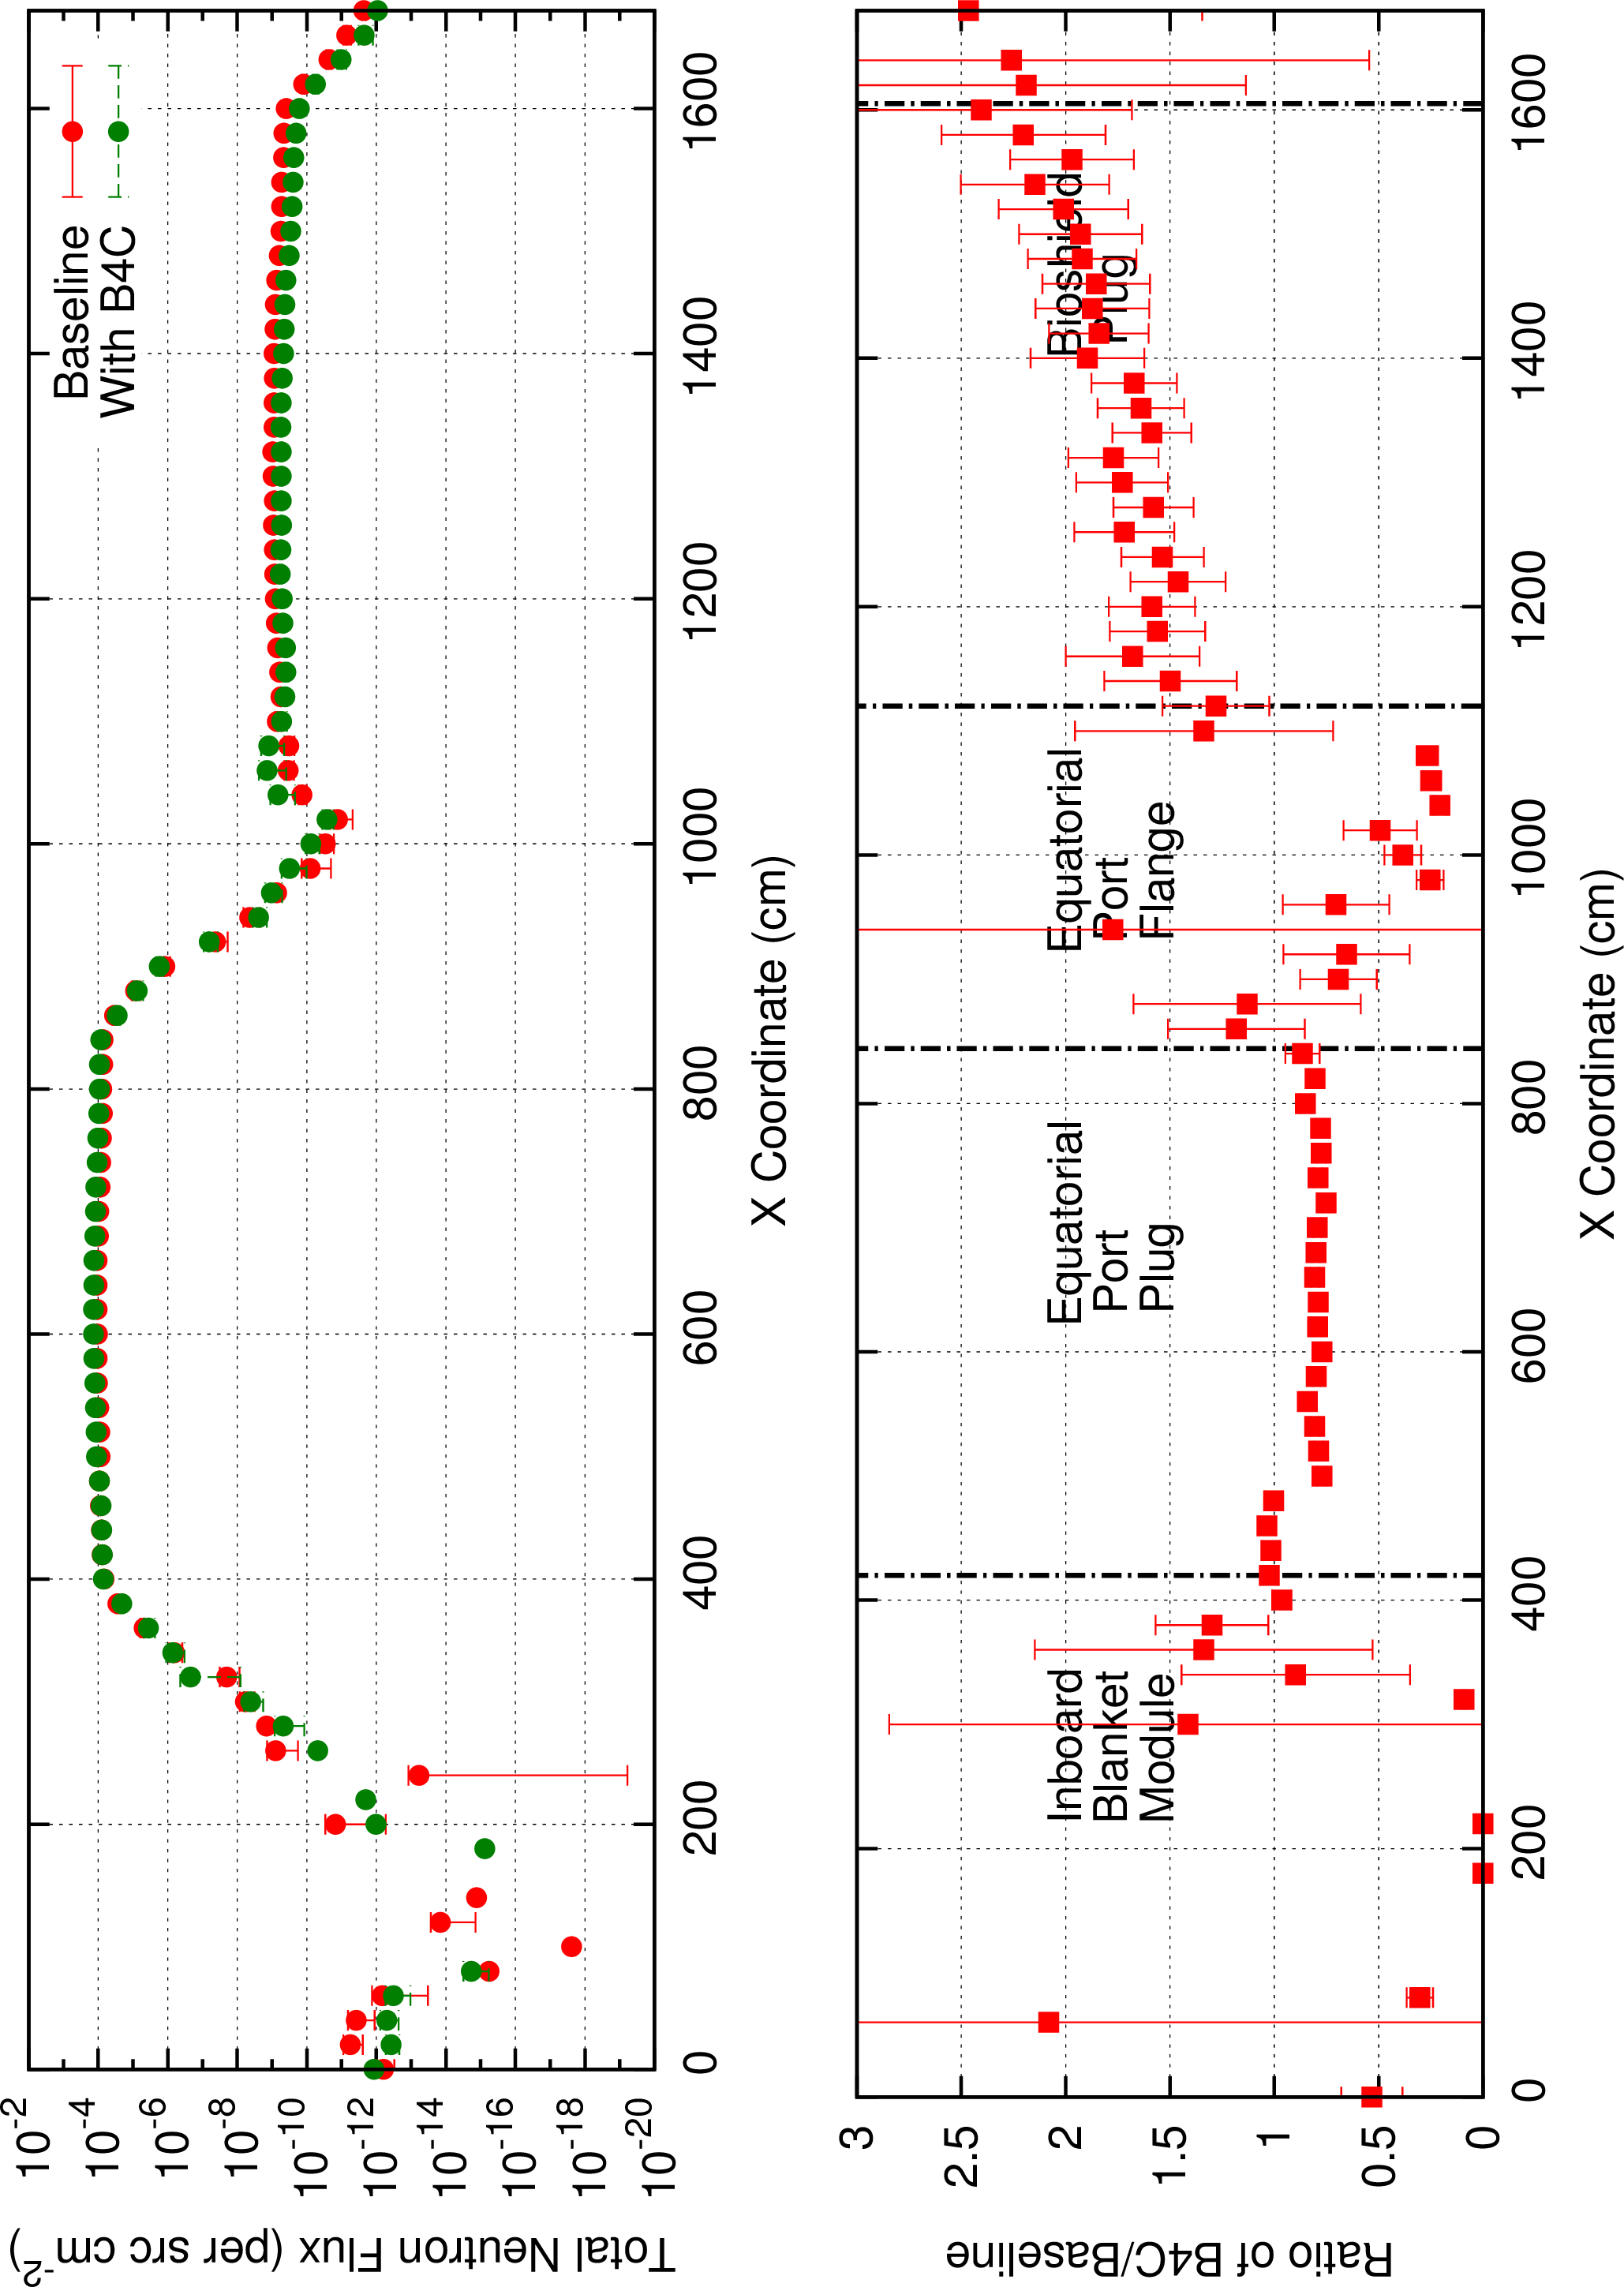
\includegraphics[angle=-90,clip,scale=0.15]{../plots/neutron/total_flux_ep.png}     
  \caption{The total flux in found along a line 0,0,0 cm to 1800,0,0 cm}
  \label{fig:total_flux_ep}
\end{figure}

As seen in Figure \ref{fig:total_flux_ep} the total flux is clearly higher in 
the baseline case than in the B$_4$C case, with increasing differences seen
beyond 1200 cm until the bioshield is reached, where the difference drops
\\
\\
The upper port can is similarly examined in Figure \ref{fig:total_flux_up},
similar features can be seen.
\begin{figure}[ht!]
  \centering
  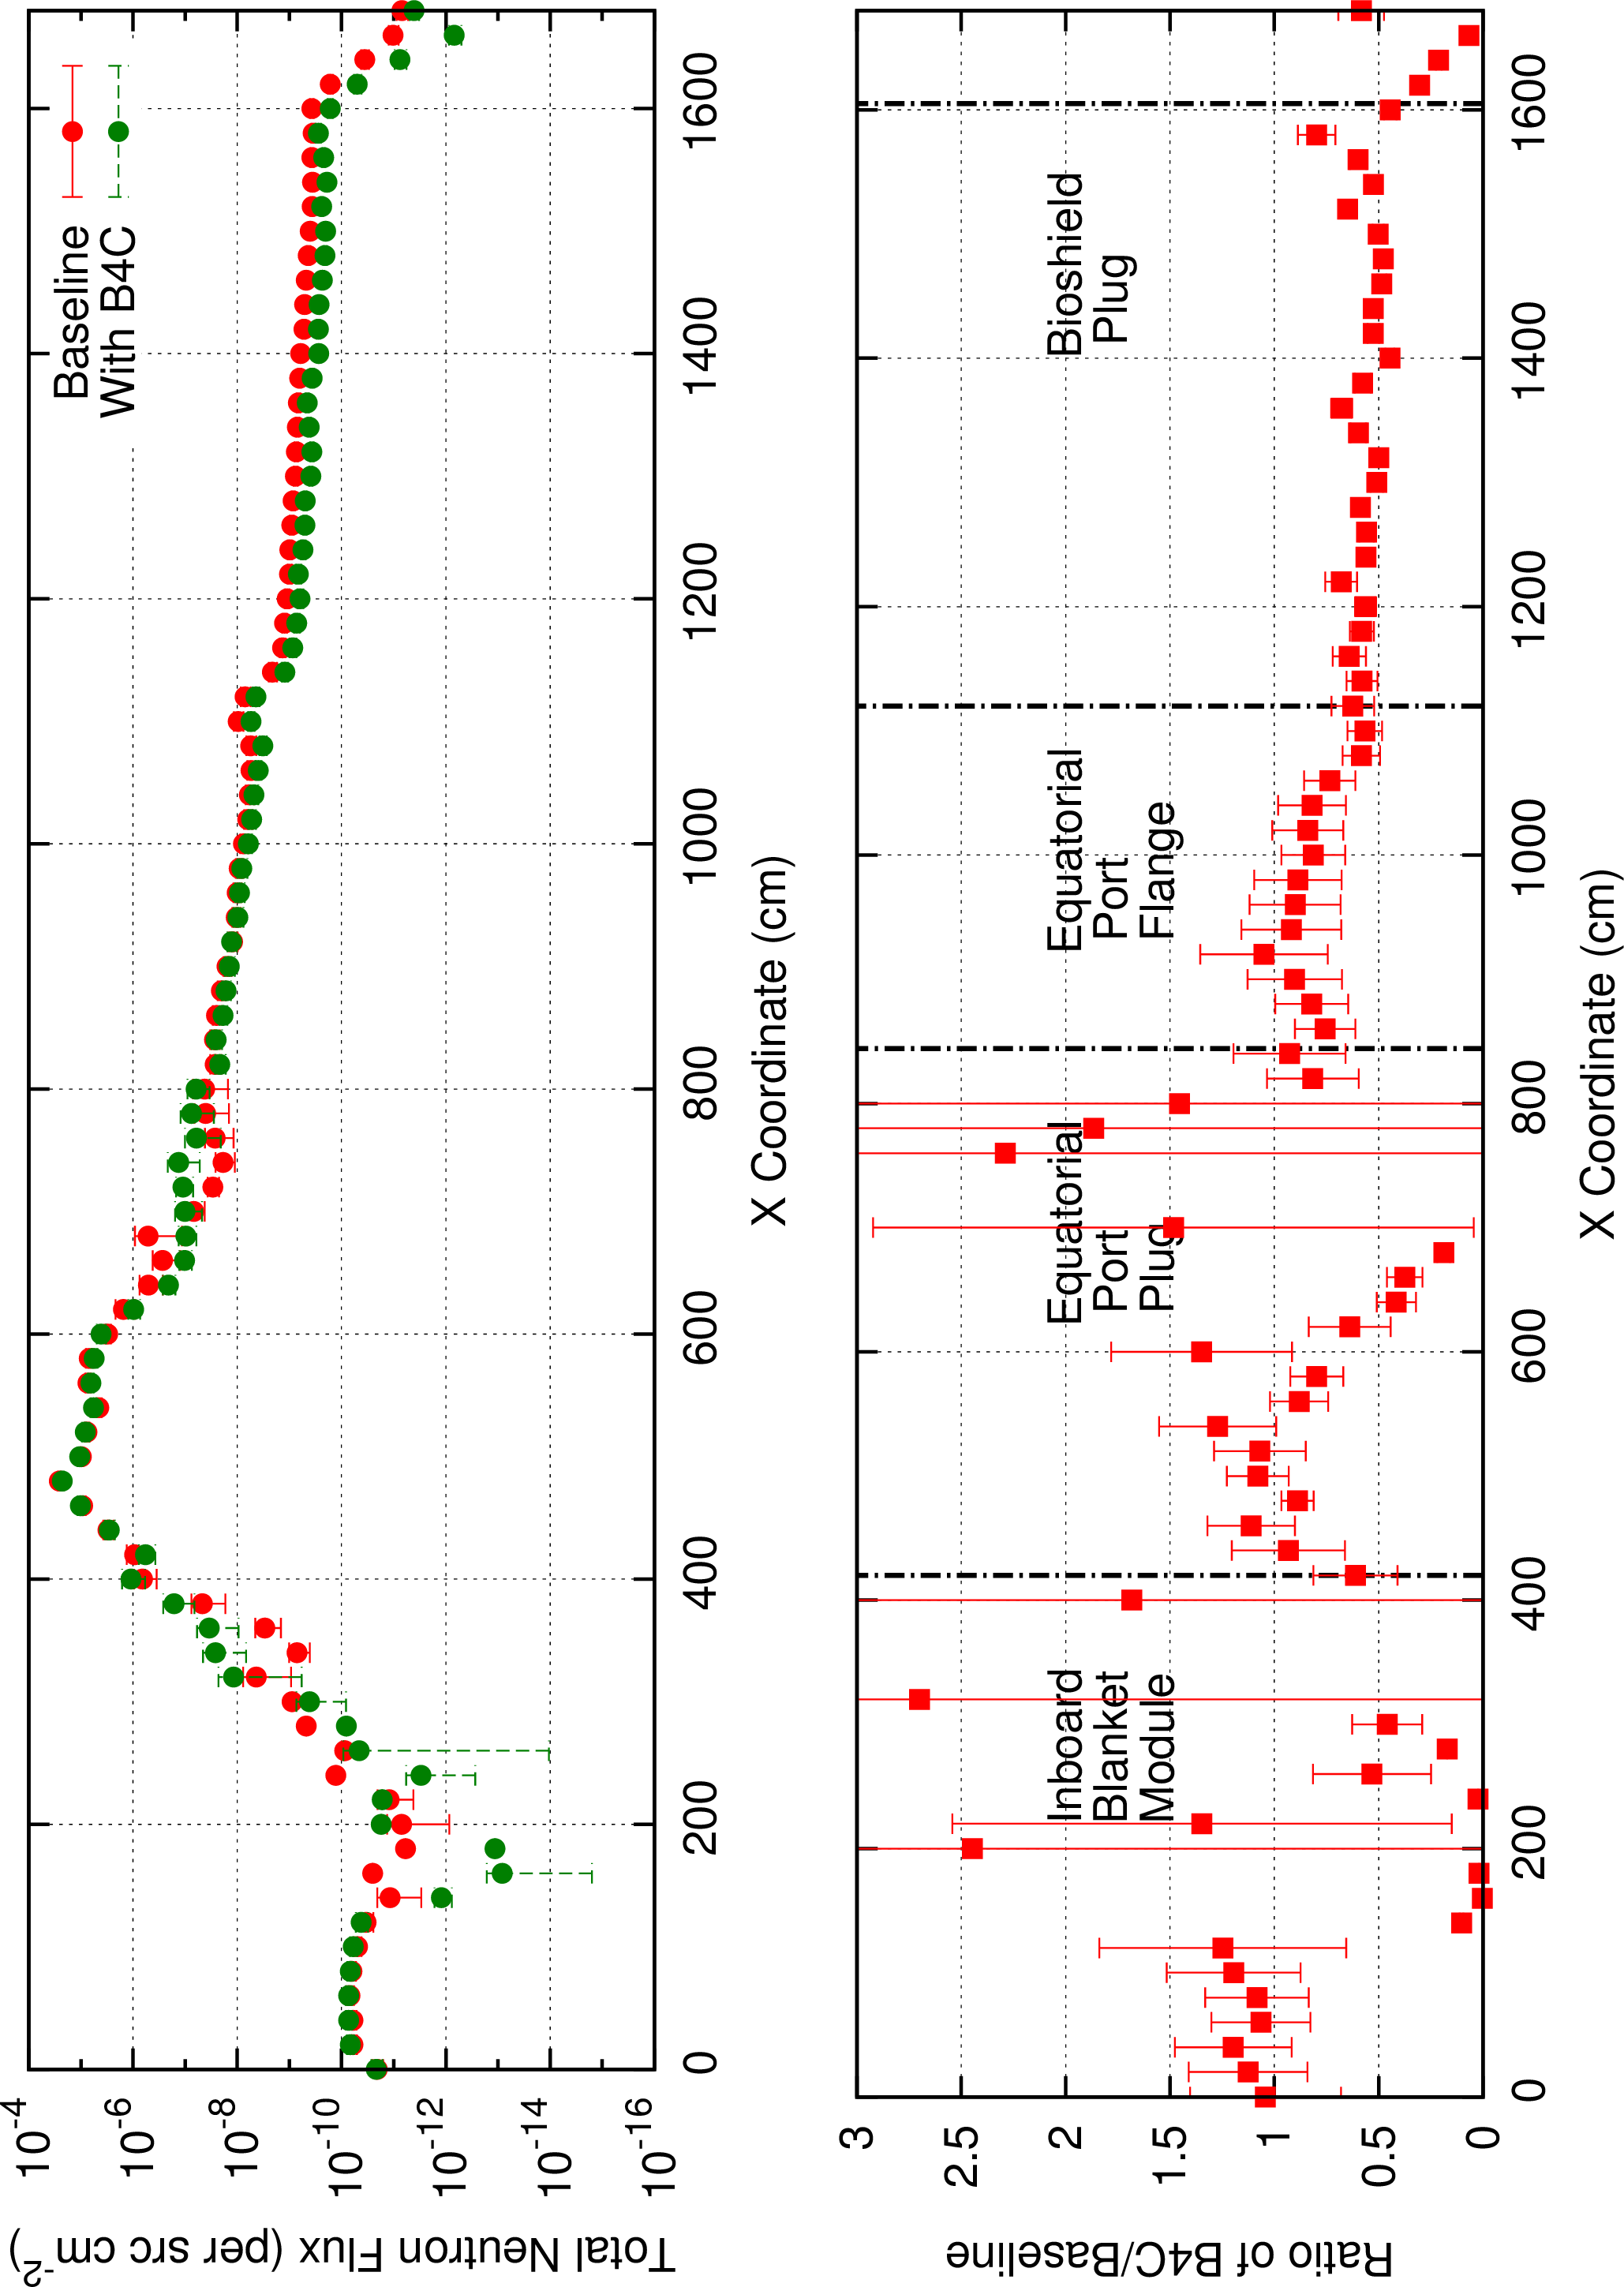
\includegraphics[angle=-90,clip,scale=0.15]{../plots/neutron/total_flux_up.png}     
  \caption{The total flux in found along a line 0,0,500 cm to 1800,0,500 cm}
  \label{fig:total_flux_up}
\end{figure}
We see that there is increasing effect in the B$_4$C closer to the bioshield, peaking
at a factor of two reduction in neutron flux.

\textbf{placeholder for lineouts for thermal and fast flux}

%% NOTE [PPHW]: Can we generate line-out plots for the neutron flux
%% (total? thermal?) like we are doing for the dose?

\subsection{Conclusion}

\textbf{placeholder for conclusion}
%% NOTE [PPHW]: Do we really need a conclusion section here?  If so, it should
%% probably focus on some discusison of the relative neutron fluxes per the
%% above request for line out plots.  That is, do we see any evidence of the
%% B4C in the neutron transport results?  

\newpage
\clearpage

\section{Neutron Activation Results and Conclusions}
\subsection{Calculation Details}
The \gls{r2s} shutdown dose rate calculations were performed using the
\texttt{pyne.r2s} methods found \gls{pyne}. The setup scripts produce
\gls{alara_c} inputs and the neutron activation calculations were performed
using \gls{alara_c} 2.9.1RC. There was an activation calculation for each 
neutron mesh and case, therefore
there were a total of fourteen activation calculations performed. The activation
calculations used a uniform `truncation tolerance', a parameter in \gls{alara_c}
which details when the linearised transmutation chains should be terminated. The
materials used in the activation calculation were taken directly from the 
associated MCNP input decks. 

\subsection{Baseline}

The total photon source intensities for the baseline case and for each decay
time are shown in Figures \ref{fig:source_dc1_no4bc}
through \ref{fig:source_dc3_no4bc}.  Figures that show the source intensity
for each of the 24 photon groups are in
appendix \ref{appendix:grp_photon_src_baseline}.  The first wall and blanket modules
clearly have the strongest source, 3-4 orders of magnitude larger than most
ex-vessel components.

\subsubsection{Decay Time 1 - $10^{5}$ seconds}
\begin{figure}[ht!]
\centering
\includegraphics[trim={0cm 9cm 0cm 10cm},clip,scale=0.75]{../plots/final_model/{Photon_Source_Density_Decay_Time_1_All_Energy_Groups}.png}
\label{fig:source_dc1_no4bc}
\caption{The total shutdown photon source for the baseline case for decay time 1}
\end{figure}
\clearpage
\subsubsection{Decay Time 2 - $10^{6}$ seconds}
\begin{figure}[ht!]
\centering
\includegraphics[trim={0cm 9cm 0cm 10cm},clip,scale=0.75]{../plots/final_model/{Photon_Source_Density_Decay_Time_2_All_Energy_Groups}.png}
\label{fig:source_dc2_no4bc}
\caption{The total shutdown photon source for the baseline case for decay time 2}
\end{figure}
\clearpage
\subsubsection{Decay Time 3 - $10^{7}$ seconds}
\begin{figure}[ht!]
\centering
\includegraphics[trim={0cm 9cm 0cm 10cm},clip,scale=0.75]{../plots/final_model/{Photon_Source_Density_Decay_Time_3_All_Energy_Groups}.png}
\label{fig:source_dc3_no4bc}
\caption{The total shutdown photon source for the baseline case for decay time 3}
\end{figure}

\newpage
\clearpage
\subsection{Including the B4C Liner}

The total photon source intensities for the case with B$_4$C liner and for
each decay time are shown in Figures \ref{fig:source_dc1_b4c}
through \ref{fig:source_dc3_b4c}.  Figures that show the source intensity for
each of the 24 photon groups are in
appendix \ref{appendix:grp_photon_src_b4c}.  


\subsubsection{Decay Time 1 - $10^{5}$ seconds}
\begin{figure}[ht!]
\centering
\includegraphics[trim={0cm 9cm 0cm 10cm},clip,scale=0.75]{../plots/final_model_with_b4c/{Photon_Source_Density_Decay_Time_1_All_Energy_Groups}.png}
\caption{The total shutdown photon source for the case with B$_4$C for decay time 1}
\label{fig:source_dc1_b4c}
\end{figure}
\clearpage
\subsubsection{Decay Time 2 - $10^{6}$ seconds}
\begin{figure}[ht!]
\centering
\includegraphics[trim={0cm 9cm 0cm 10cm},clip,scale=0.75]{../plots/final_model_with_b4c/{Photon_Source_Density_Decay_Time_2_All_Energy_Groups}.png}
\caption{The total shutdown photon source for the case with B$_4$C for decay time 2}
\label{fig:source_dc2_b4c}
\end{figure}
\clearpage
\subsubsection{Decay Time 3 - $10^{7}$ seconds}
\begin{figure}[ht!]
\centering
\includegraphics[trim={0cm 9cm 0cm 10cm},clip,scale=0.75]{../plots/final_model_with_b4c/{Photon_Source_Density_Decay_Time_3_All_Energy_Groups}.png}
\caption{The total shutdown photon source for the case with B$_4$C for decay time 3}
\label{fig:source_dc3_b4c}
\end{figure}

\clearpage
\subsection{Comparison}



%% NOTE [PPHW]: What do we want to say here? Anything??
%% NOTE [PPHW]: Why do the B4C results look smoother/better in the bioshield?

\subsection{Conclusion}

It is worth noting that the lack of gamma source present in the \gls{epp}
regions are not due to poor neutron transport in this region, but due to the
fact that the \gls{gepp} model has a large B$_4$C powder filled containers
in these regions, B$_4$C when irradiated by neutrons undergoes reactions
which produce only low energy beta particle decays with very low associated
photon energies, thus effectively produces no decay photons.

\newpage
\clearpage
\section{Shutdown Photon Dose rates Results and Conclusions}

\subsection{Calculation Details}
The shutdown photon sources were developed in several separate meshes and
therefore any individual mesh does not represent the entire problem. The
results of the previous \gls{alara_c} calculations are then processed further
to make shutdown sources to be read into a sampling subroutine (also distributed
with \gls{pyne}). Each photon source is run independently, and the photon dose
is recorded on a mesh common to each photon calculation and then the meshes
summed together to create the final result. The final mesh has a uniform size of
side 5 cm $\times$ 5 cm $\times$ 5.23 cm striding from x = {0,2000}, y = {-600,600},
 z = {-1500,1900} cm. The meshes used the\gls{icrp}-74 dose response coefficients 
as a dose multiplier as recommended in \cite{iter_sdr_coeffs}.
\\
\\
Each photon transport calculation was performed for a fixed number of particles,
$10^8$, which nominally completed in less than 15 hours on 40 cores of
\gls{aci}. Each photon simulation used the same random number seed, but given
that each photon source is unique, there are no concerns regarding the resuse
of the same seed.

%% NOTES [PPHW]: Need some basic discussion - at least to describe what is in
%% each figure.

\subsection{Baseline}
\subsubsection{Decay time 1 - $10^5$ s}
\begin{figure}[ht!]
\centering
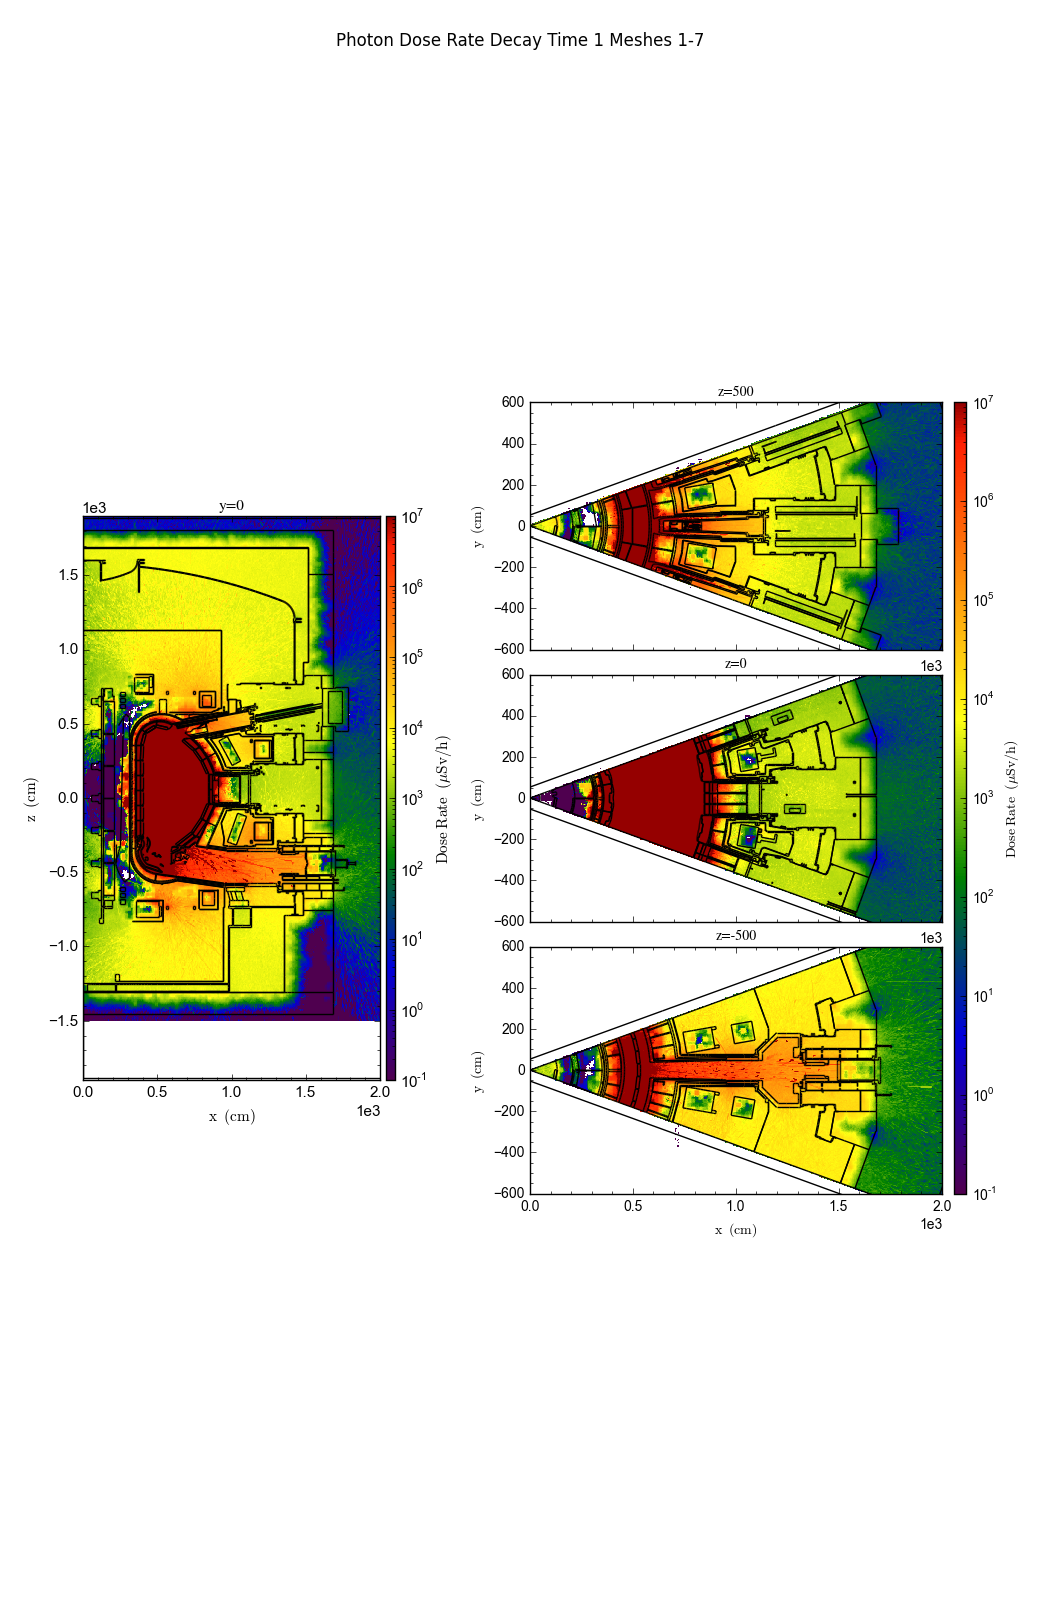
\includegraphics[trim={0cm 9cm 0cm 10cm},clip,scale=0.75]{../plots/final_model/Photon_Dose_Rate_Decay_Time_1_Meshes_1-7.png}
\caption{The total dose rate summed over all meshes for decay time 1}
\label{fig:photons_dc1_no4bc_total}
\end{figure}
\begin{figure}[ht!]
\centering
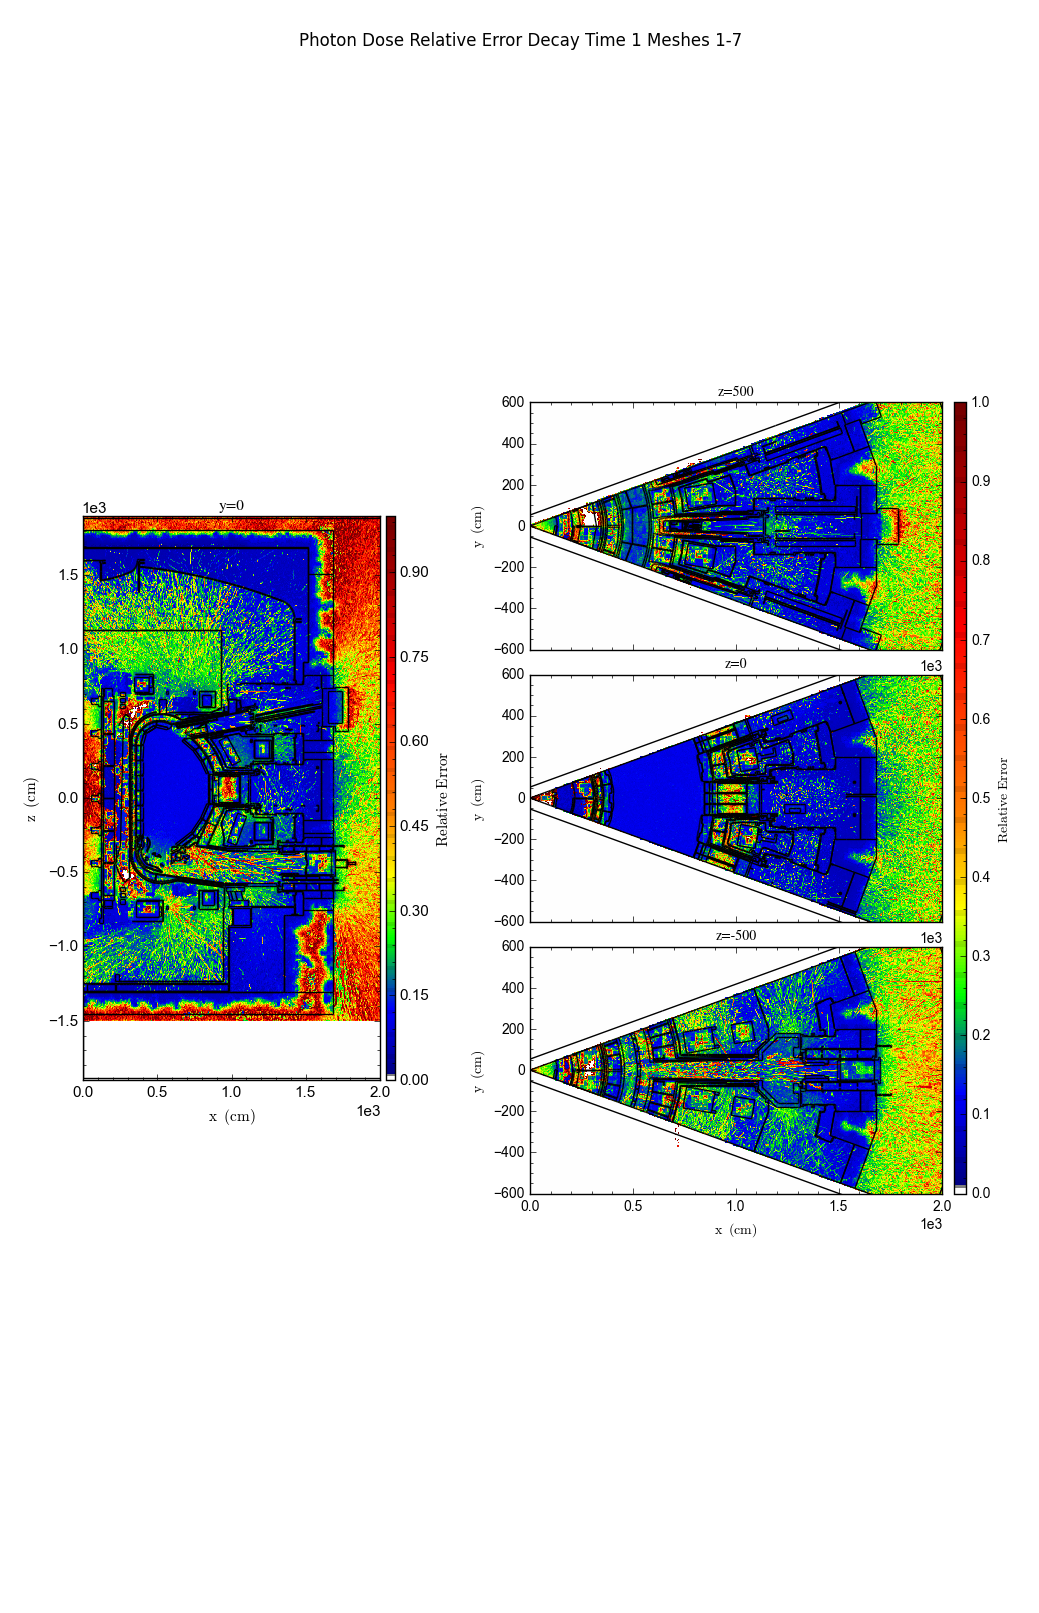
\includegraphics[trim={0cm 9cm 0cm 10cm},clip,scale=0.75]{../plots/final_model/Photon_Dose_Relative_Error_Decay_Time_1_Meshes_1-7.png}
\caption{The error in the total dose rate combined over all meshes for decay time 1}
\label{fig:photons_dc1_no4bc_total_error}
\end{figure}
\begin{figure}[ht!]
\centering
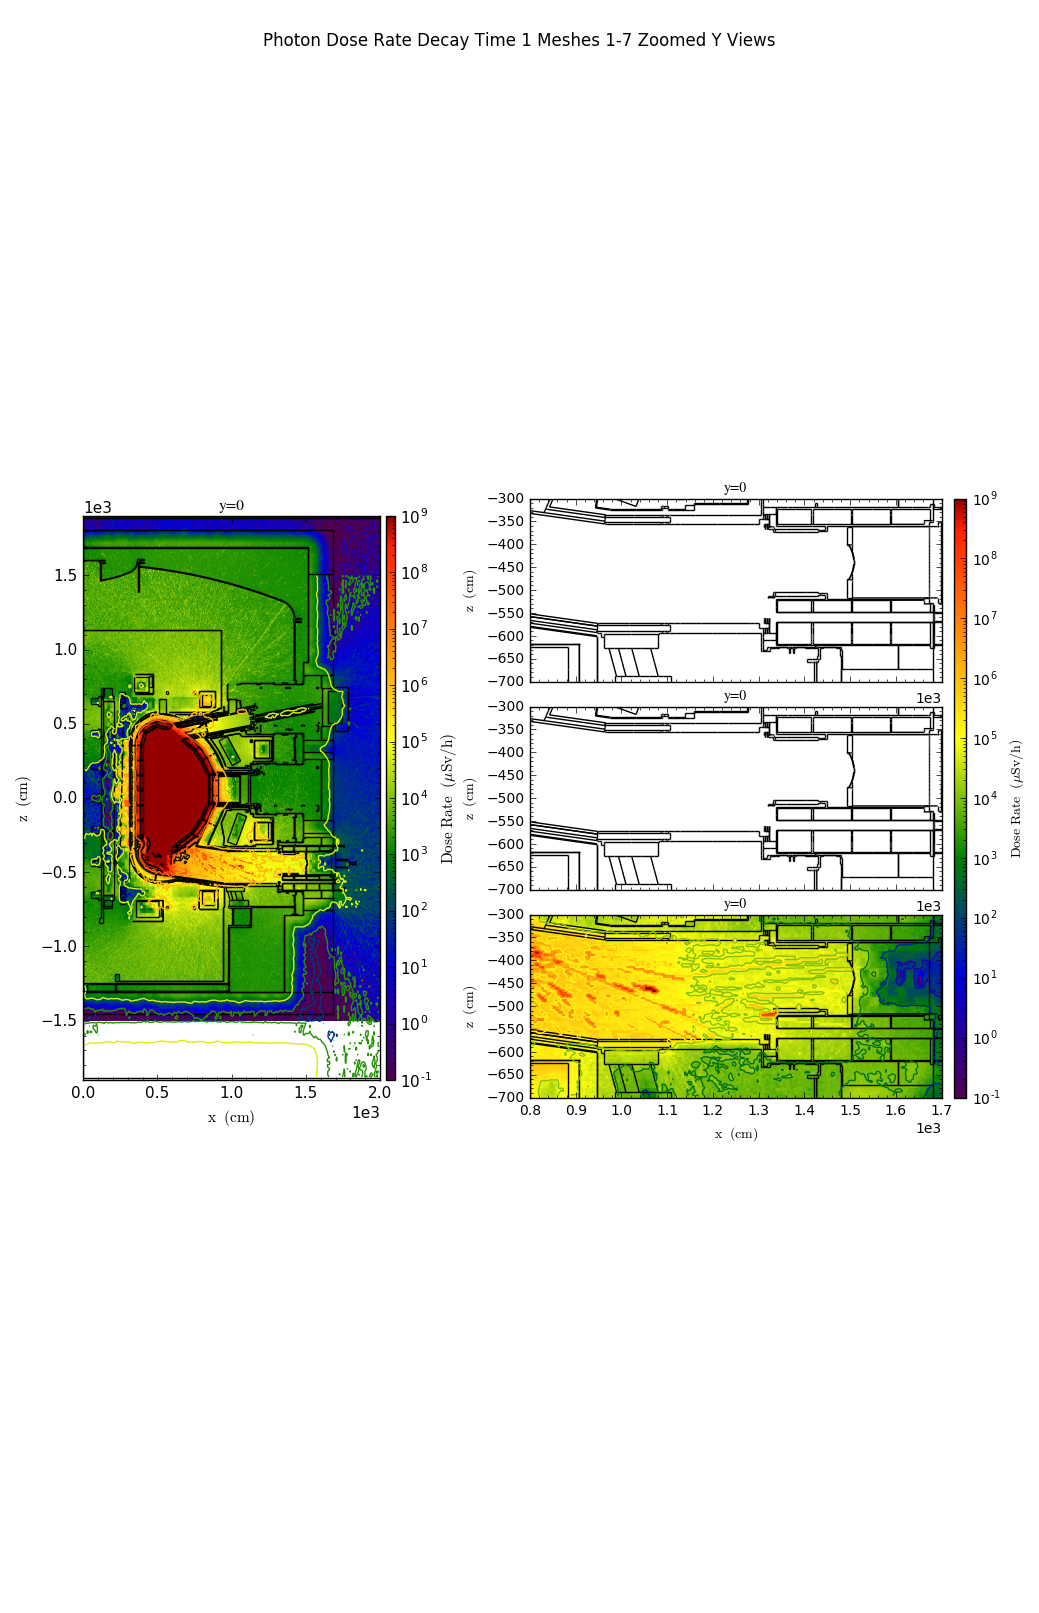
\includegraphics[trim={0cm 9cm 0cm 10cm},clip,scale=0.75]{../plots/final_model/Photon_Dose_Rate_Decay_Time_1_Meshes_1-7_Zoomed_Y_Views.png}
\caption{The total dose rate summed over all meshes for decay time 1, with focus on the port areas}
\label{fig:photons_dc1_no4bc_total_zoomed}
\end{figure}
\begin{figure}[ht!]
\centering
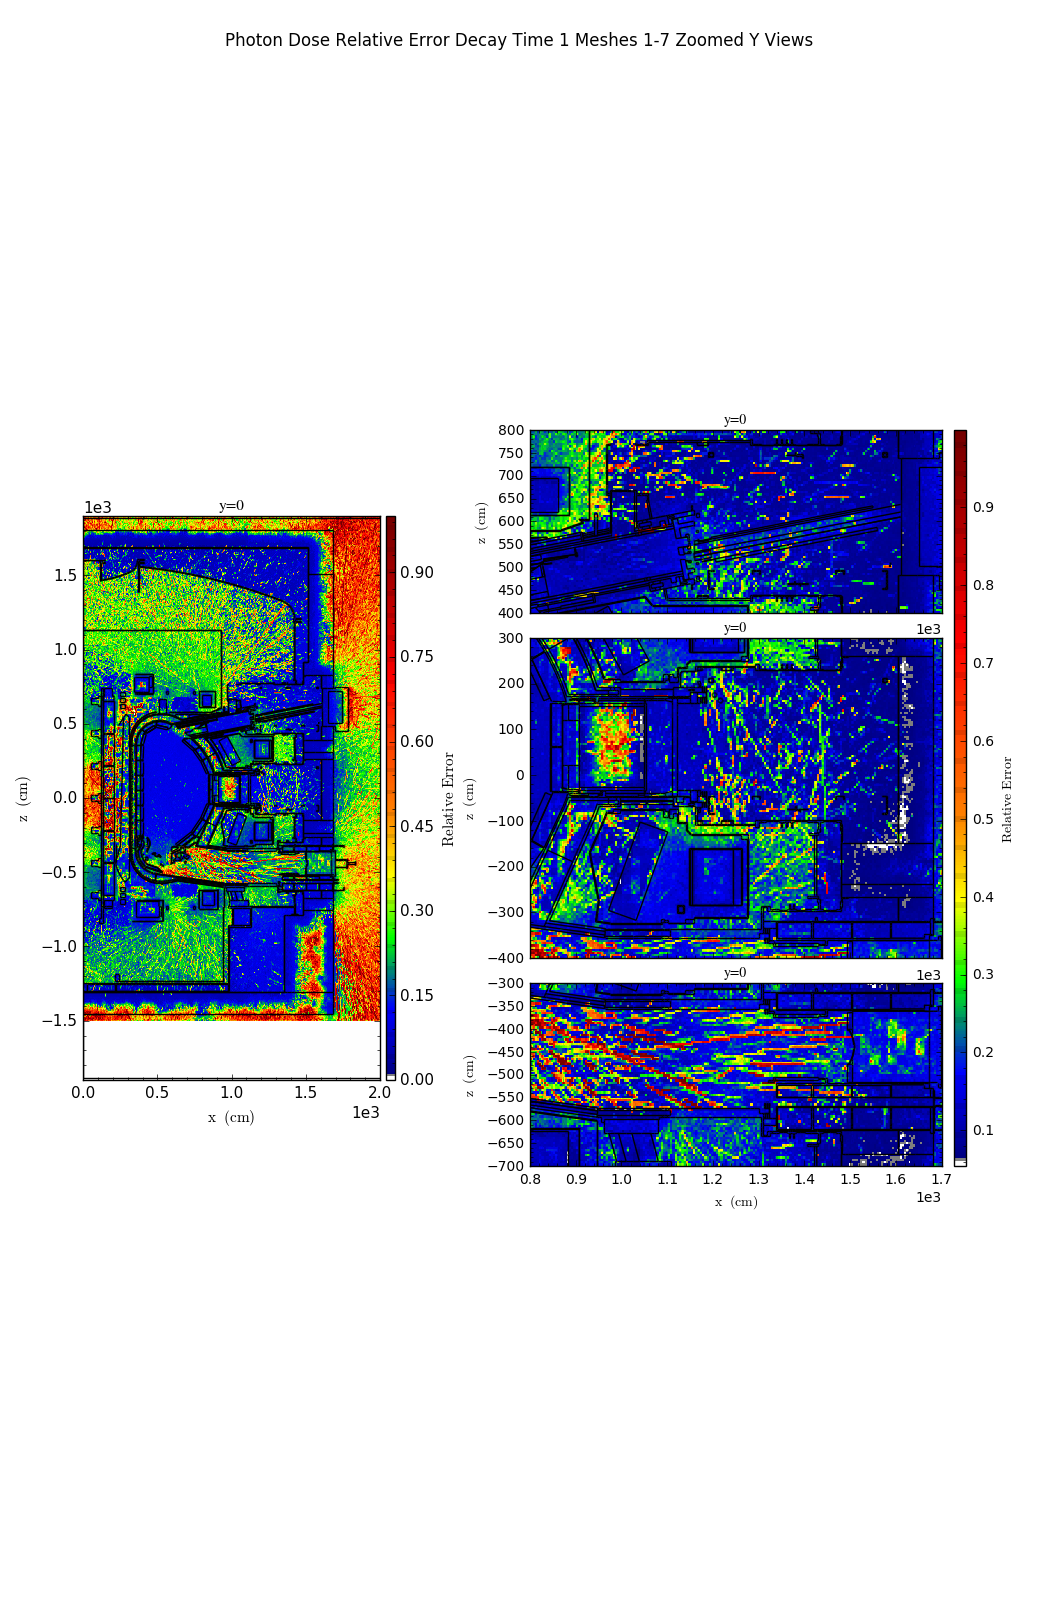
\includegraphics[trim={0cm 9cm 0cm 10cm},clip,scale=0.75]{../plots/final_model/Photon_Dose_Relative_Error_Decay_Time_1_Meshes_1-7_Zoomed_Y_Views.png}
\caption{The error in the total dose rate combined over all meshes for decay time 1, with focus on the port areas}
\label{fig:photons_dc1_no4bc_total_error_zoomed}
\end{figure}

\clearpage
\subsubsection{Decay time 2 - $10^6$ s}
%% the totals plots
\begin{figure}[ht!]
\centering
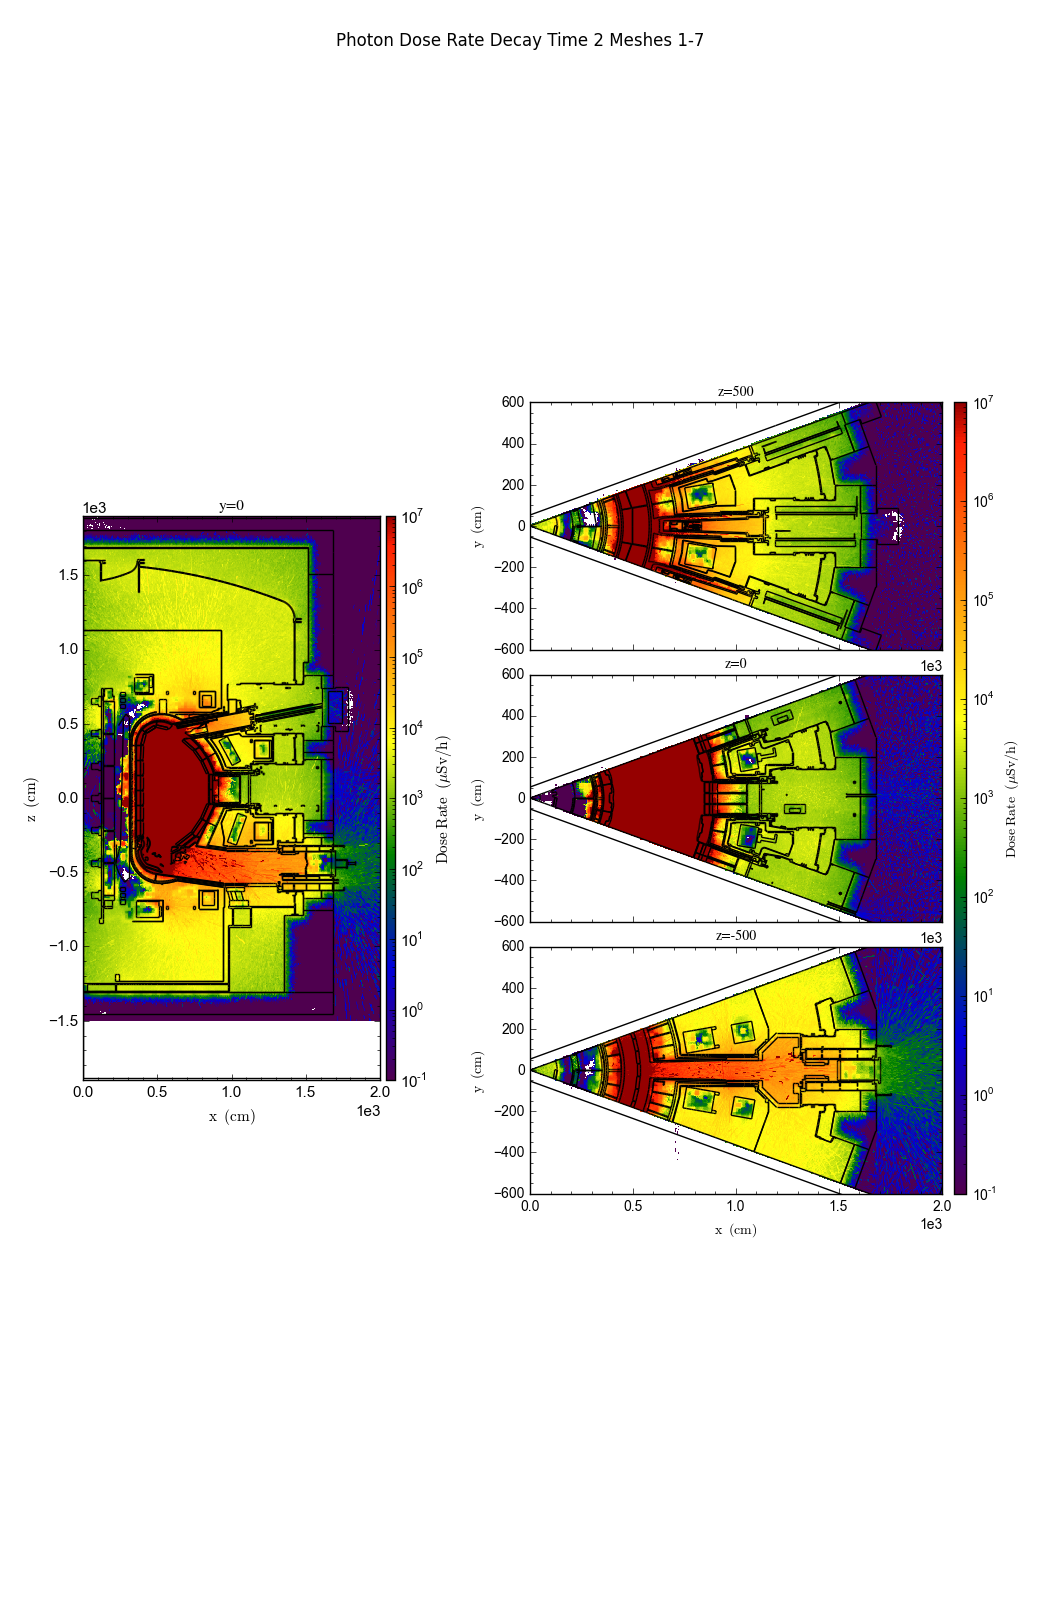
\includegraphics[trim={0cm 9cm 0cm 10cm},clip,scale=0.75]{../plots/final_model/Photon_Dose_Rate_Decay_Time_2_Meshes_1-7.png}
\caption{The total dose rate summed over all meshes for decay time 2}
\label{fig:photons_dc2_no4bc_total}
\end{figure}
\begin{figure}[ht!]
\centering
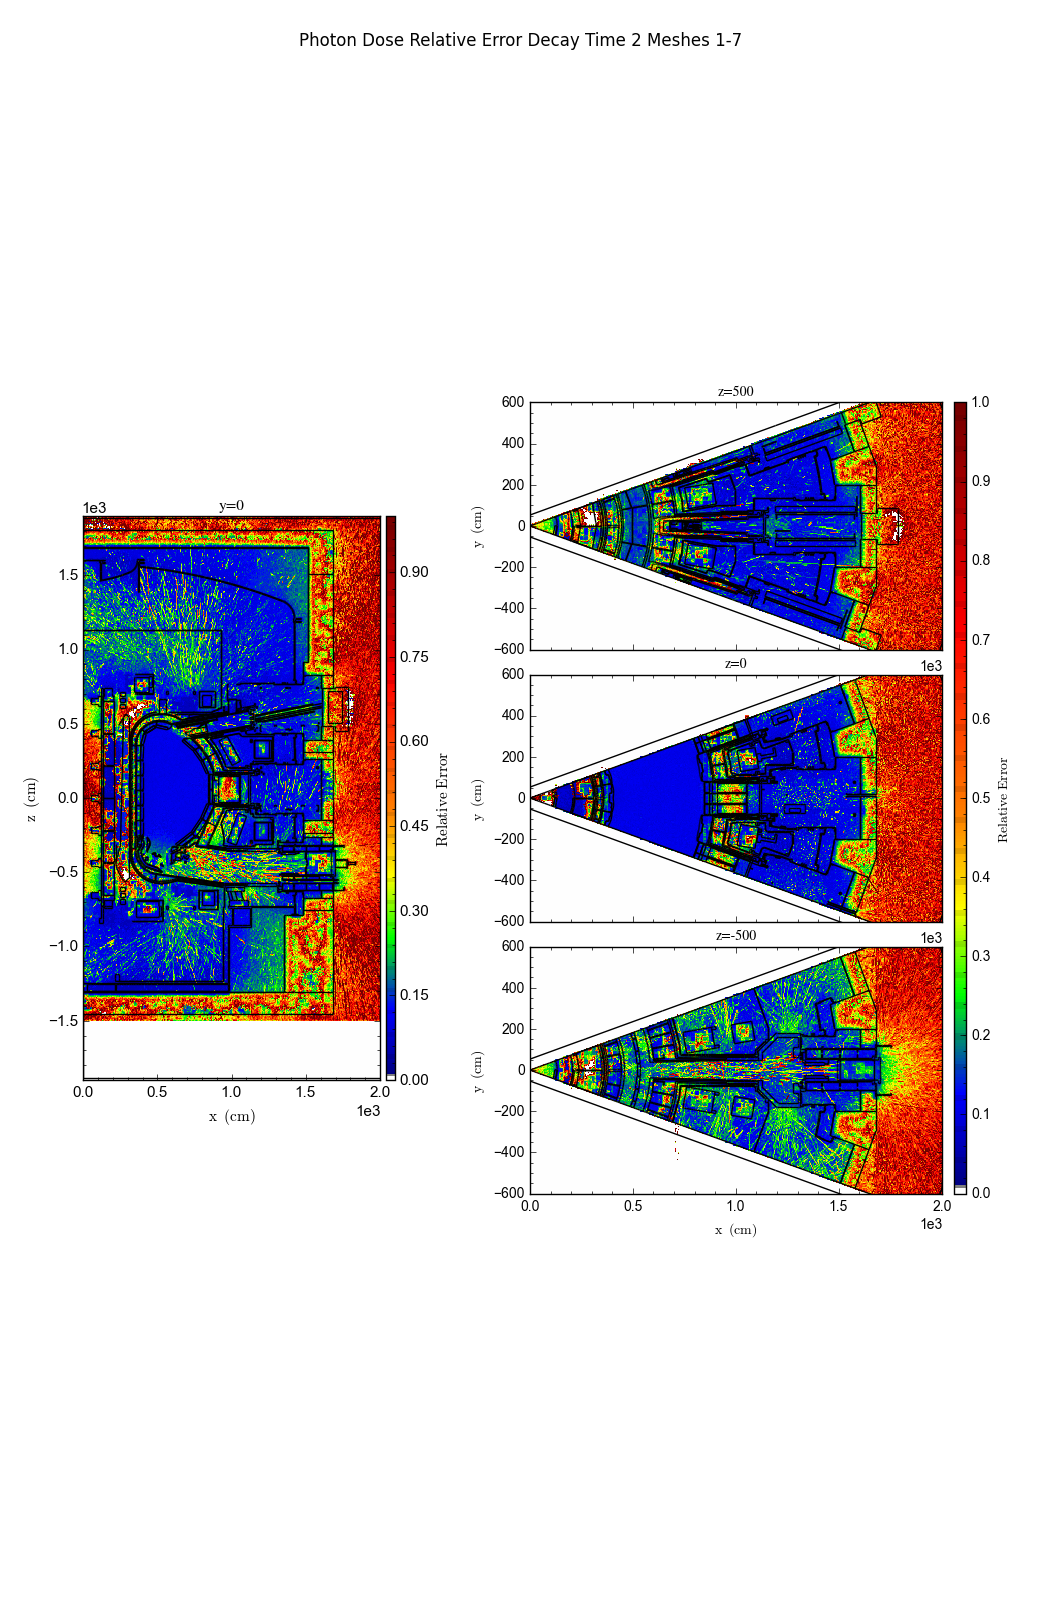
\includegraphics[trim={0cm 9cm 0cm 10cm},clip,scale=0.75]{../plots/final_model/Photon_Dose_Relative_Error_Decay_Time_2_Meshes_1-7.png}
\caption{The error in the total dose rate combined over all meshes for decay time 2}
\label{fig:photons_dc2_no4bc_total_error}
\end{figure}
\begin{figure}[ht!]
\centering
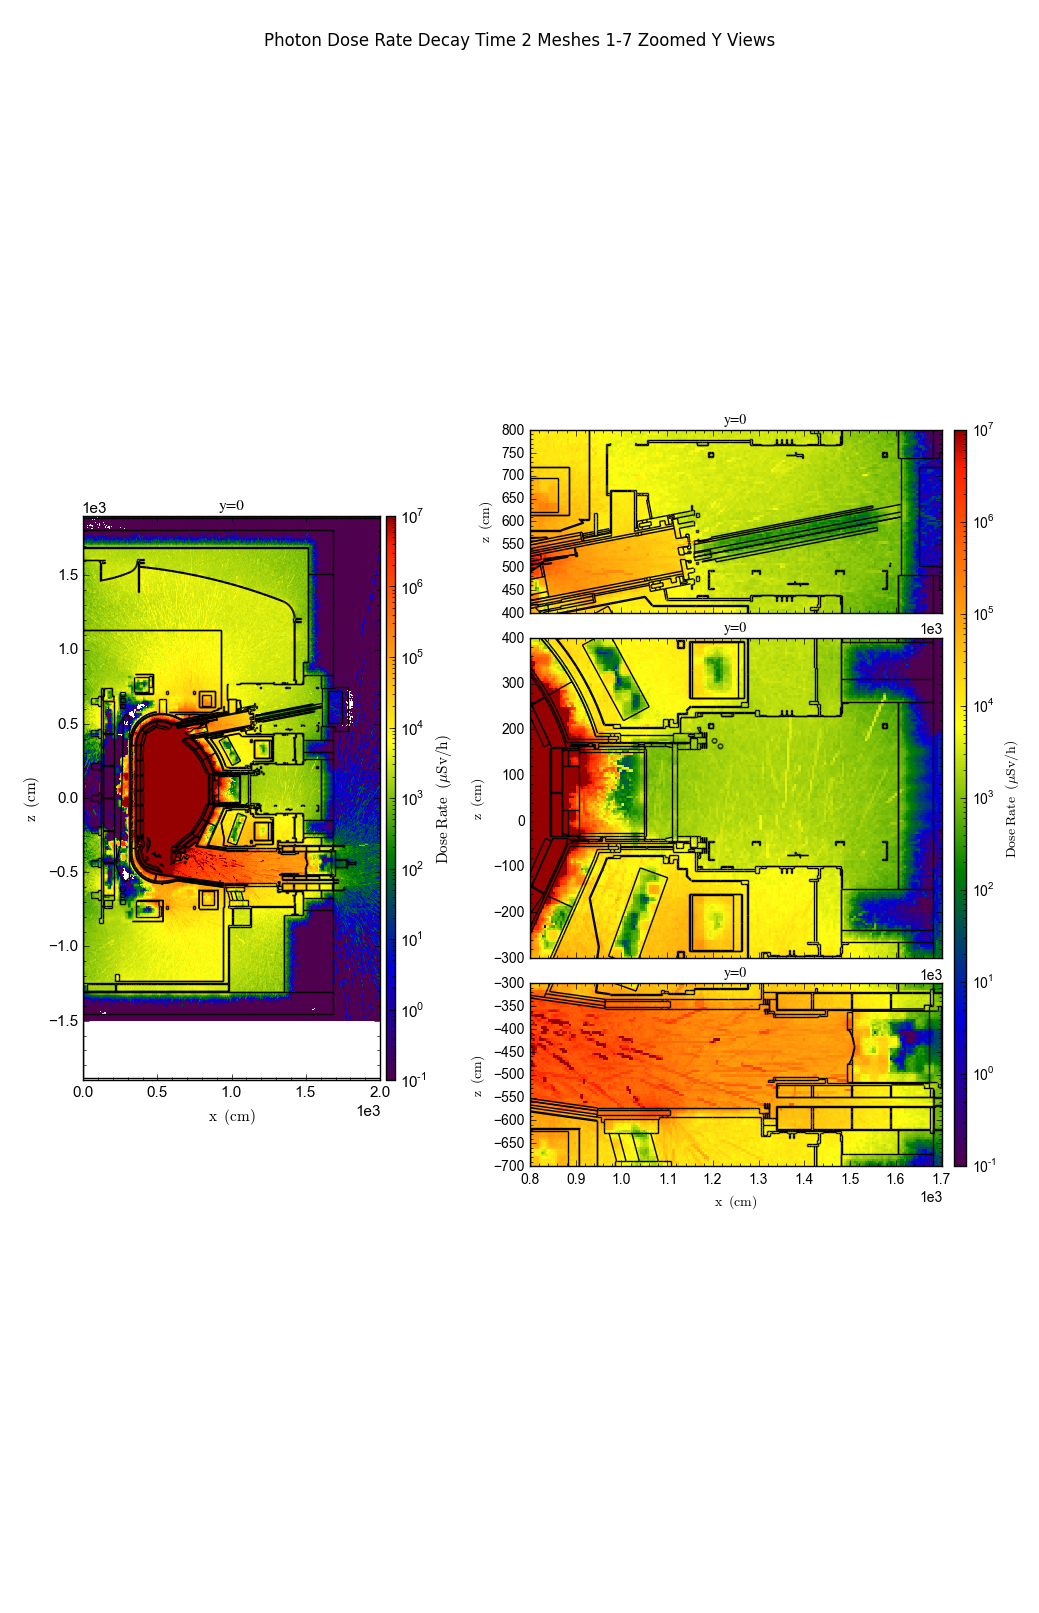
\includegraphics[trim={0cm 9cm 0cm 10cm},clip,scale=0.75]{../plots/final_model/Photon_Dose_Rate_Decay_Time_2_Meshes_1-7_Zoomed_Y_Views.png}
\caption{The total dose rate summed over all meshes for decay time 2, with focus on the port areas}
\label{fig:photons_dc2_no4bc_total_zoomed}
\end{figure}
\begin{figure}[ht!]
\centering
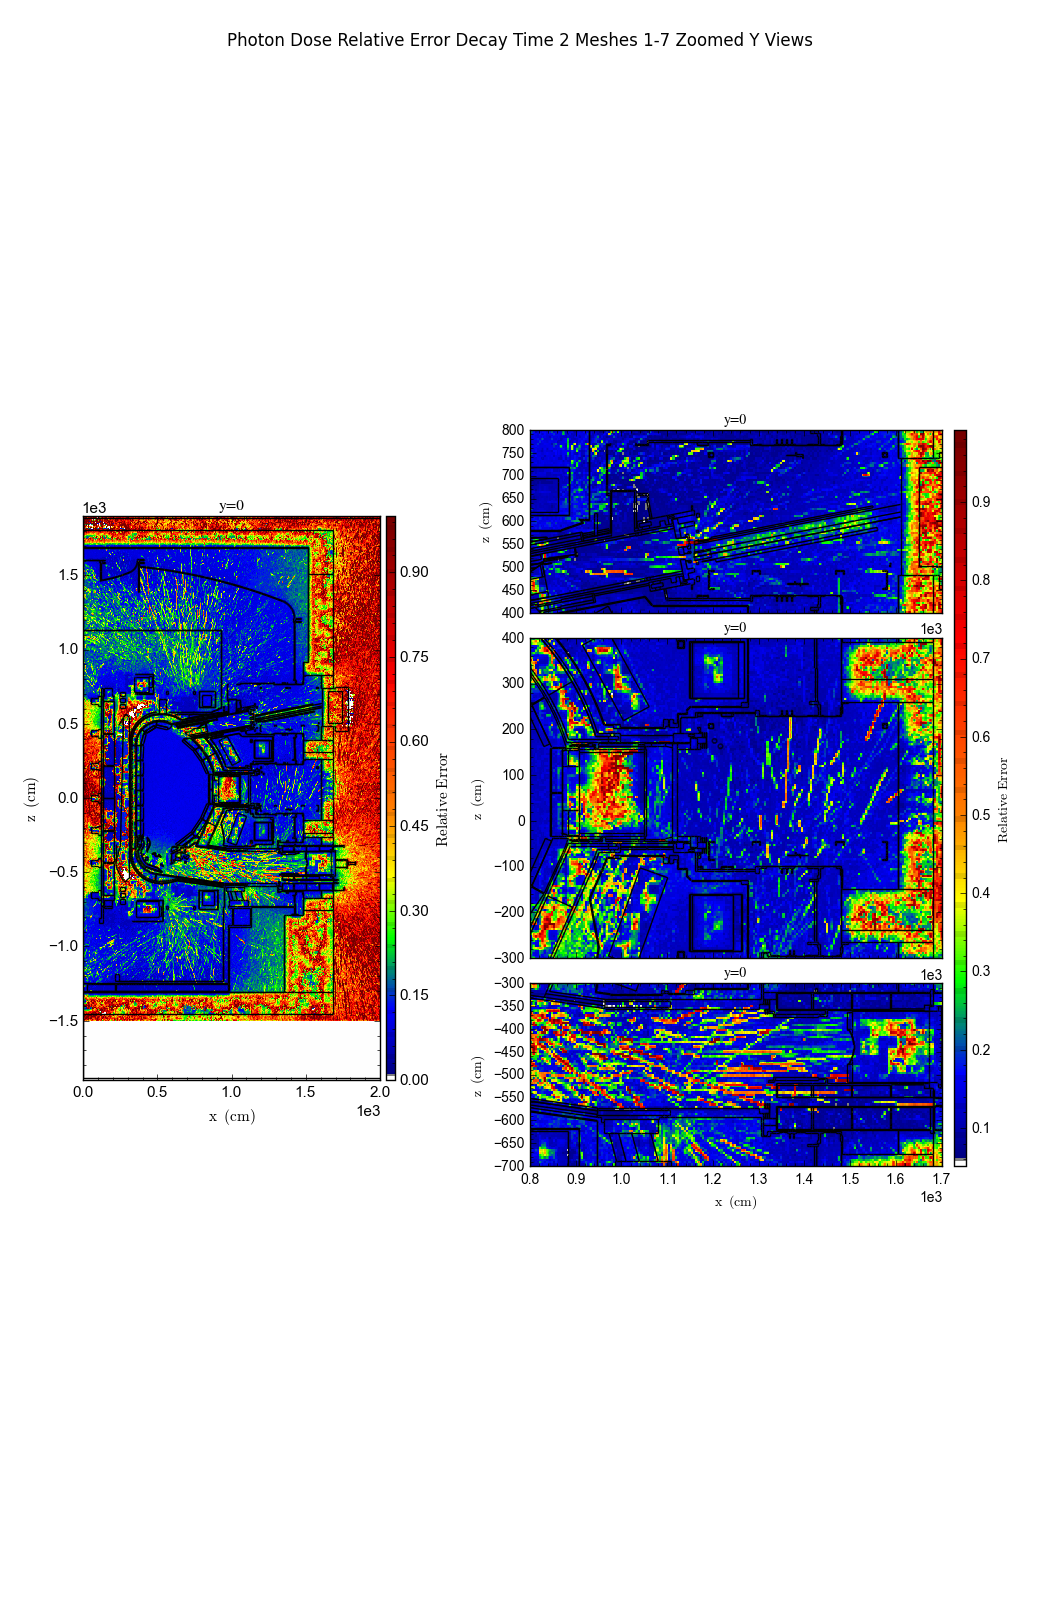
\includegraphics[trim={0cm 9cm 0cm 10cm},clip,scale=0.75]{../plots/final_model/Photon_Dose_Relative_Error_Decay_Time_2_Meshes_1-7_Zoomed_Y_Views.png}
\caption{The error in the total dose rate combined over all meshes for decay time 2, with focus on the port areas}
\label{fig:photons_dc2_no4bc_total_error_zoomed}
\end{figure}
\clearpage

\subsubsection{Decay time 3 - $10^7$ s}
%% the totals plots
\begin{figure}[ht!]
\centering
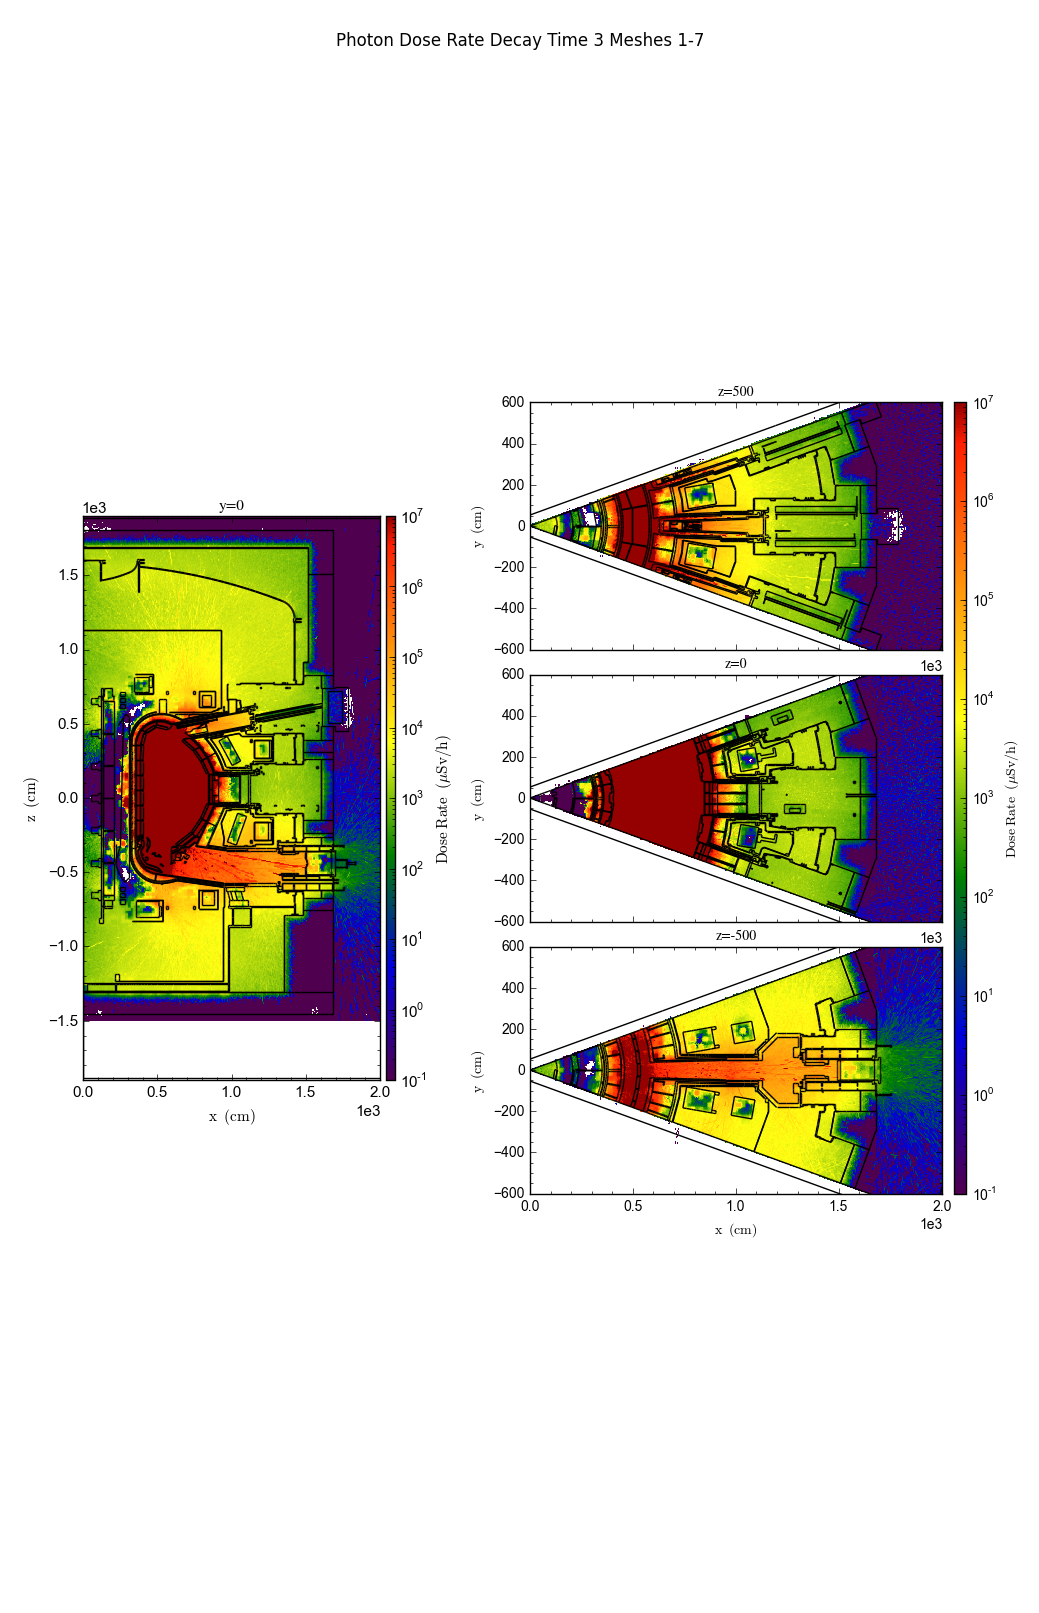
\includegraphics[trim={0cm 9cm 0cm 10cm},clip,scale=0.75]{../plots/final_model/Photon_Dose_Rate_Decay_Time_3_Meshes_1-7.png}
\caption{The total dose rate summed over all meshes for decay time 3}
\label{fig:photons_dc3_no4bc_total}
\end{figure}
\begin{figure}[ht!]
\centering
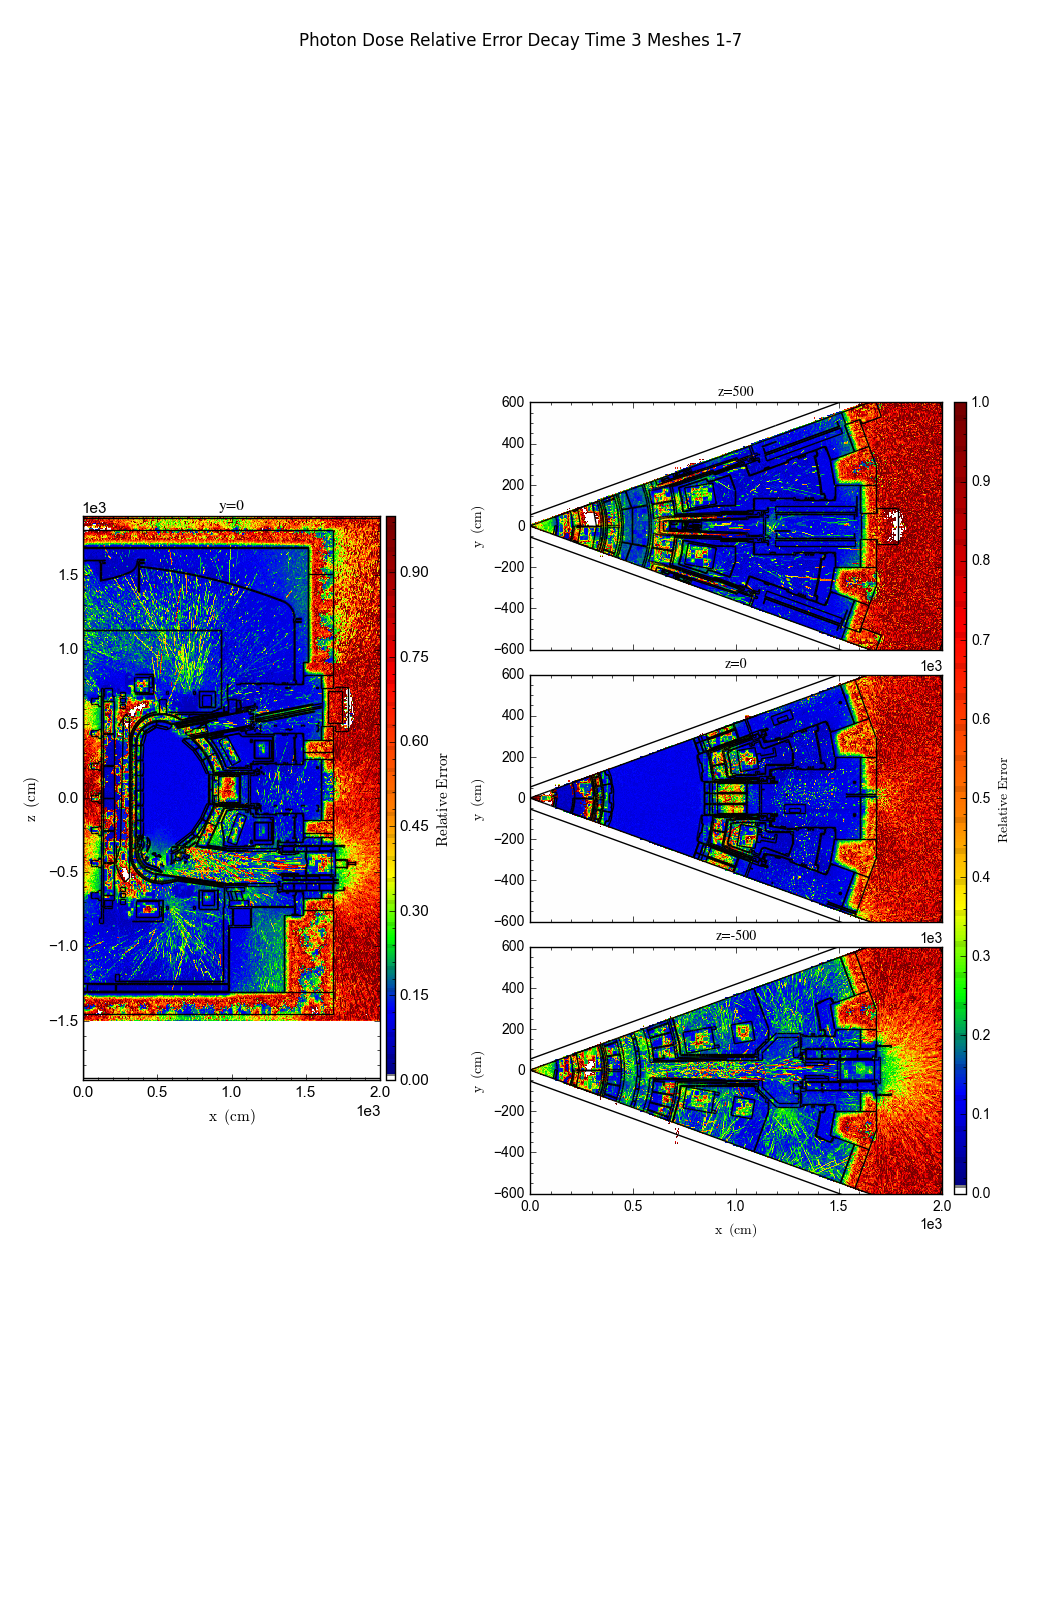
\includegraphics[trim={0cm 9cm 0cm 10cm},clip,scale=0.75]{../plots/final_model/Photon_Dose_Relative_Error_Decay_Time_3_Meshes_1-7.png}
\caption{The error in the total dose rate combined over all meshes for decay time 3}
\label{fig:photons_dc3_no4bc_total_error}
\end{figure}
\begin{figure}[ht!]
\centering
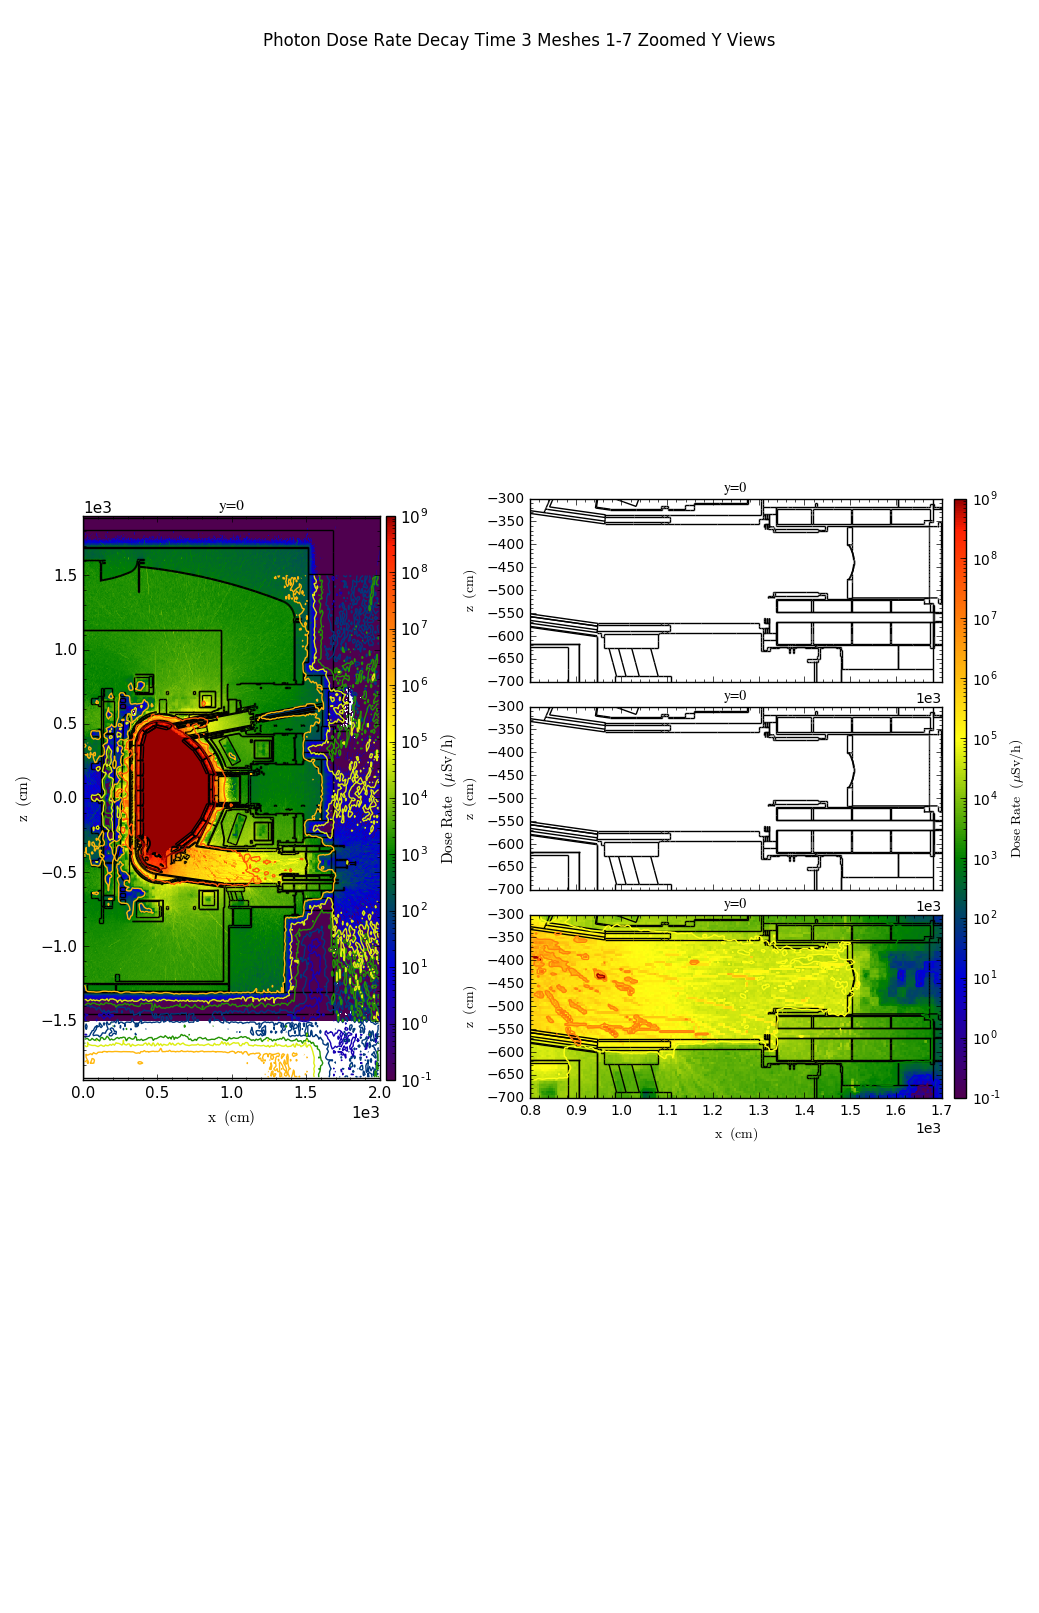
\includegraphics[trim={0cm 9cm 0cm 10cm},clip,scale=0.75]{../plots/final_model/Photon_Dose_Rate_Decay_Time_3_Meshes_1-7_Zoomed_Y_Views.png}
\caption{The total dose rate summed over all meshes for decay time 3, with focus on the port areas}
\label{fig:photons_dc3_no4bc_total_zoomed}
\end{figure}
\begin{figure}[ht!]
\centering
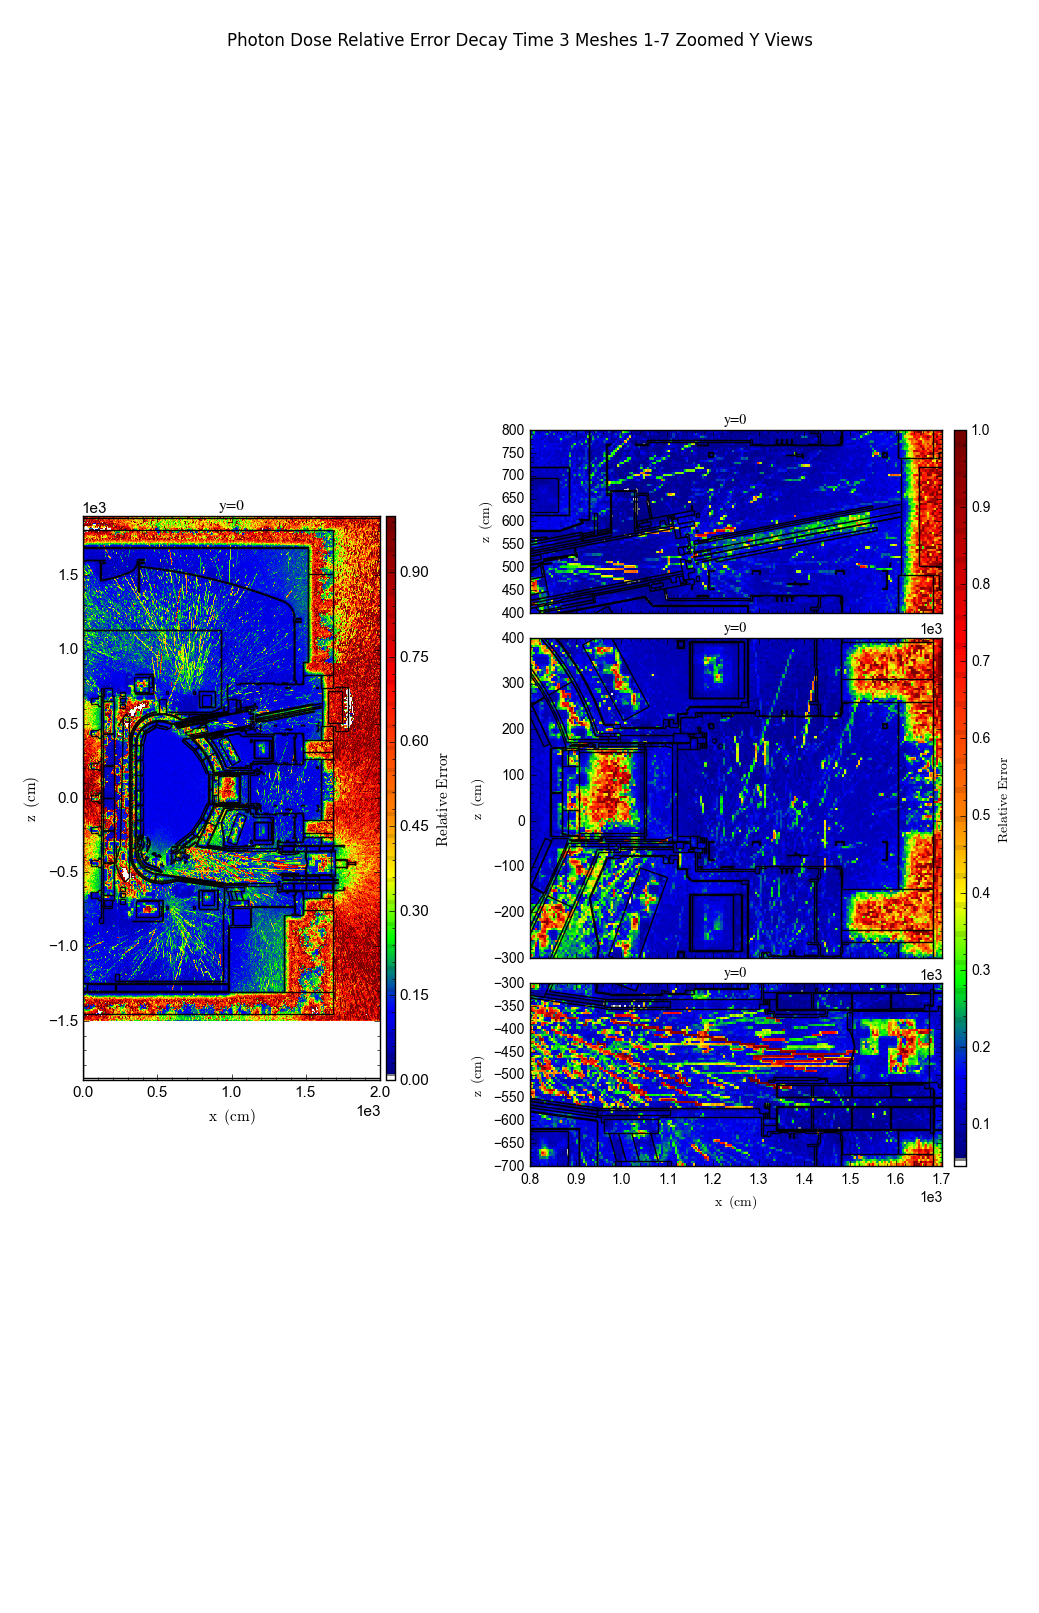
\includegraphics[trim={0cm 9cm 0cm 10cm},clip,scale=0.75]{../plots/final_model/Photon_Dose_Relative_Error_Decay_Time_3_Meshes_1-7_Zoomed_Y_Views.png}
\caption{The error in the total dose rate combined over all meshes for decay time 3, with focus on the port areas}
\label{fig:photons_dc3_no4bc_total_error_zoomed}
\end{figure}
\clearpage
\subsection{Including the B$_4$C liner}
\subsubsection{Decay time 1 - $10^5$ s}
\begin{figure}[ht!]
\centering
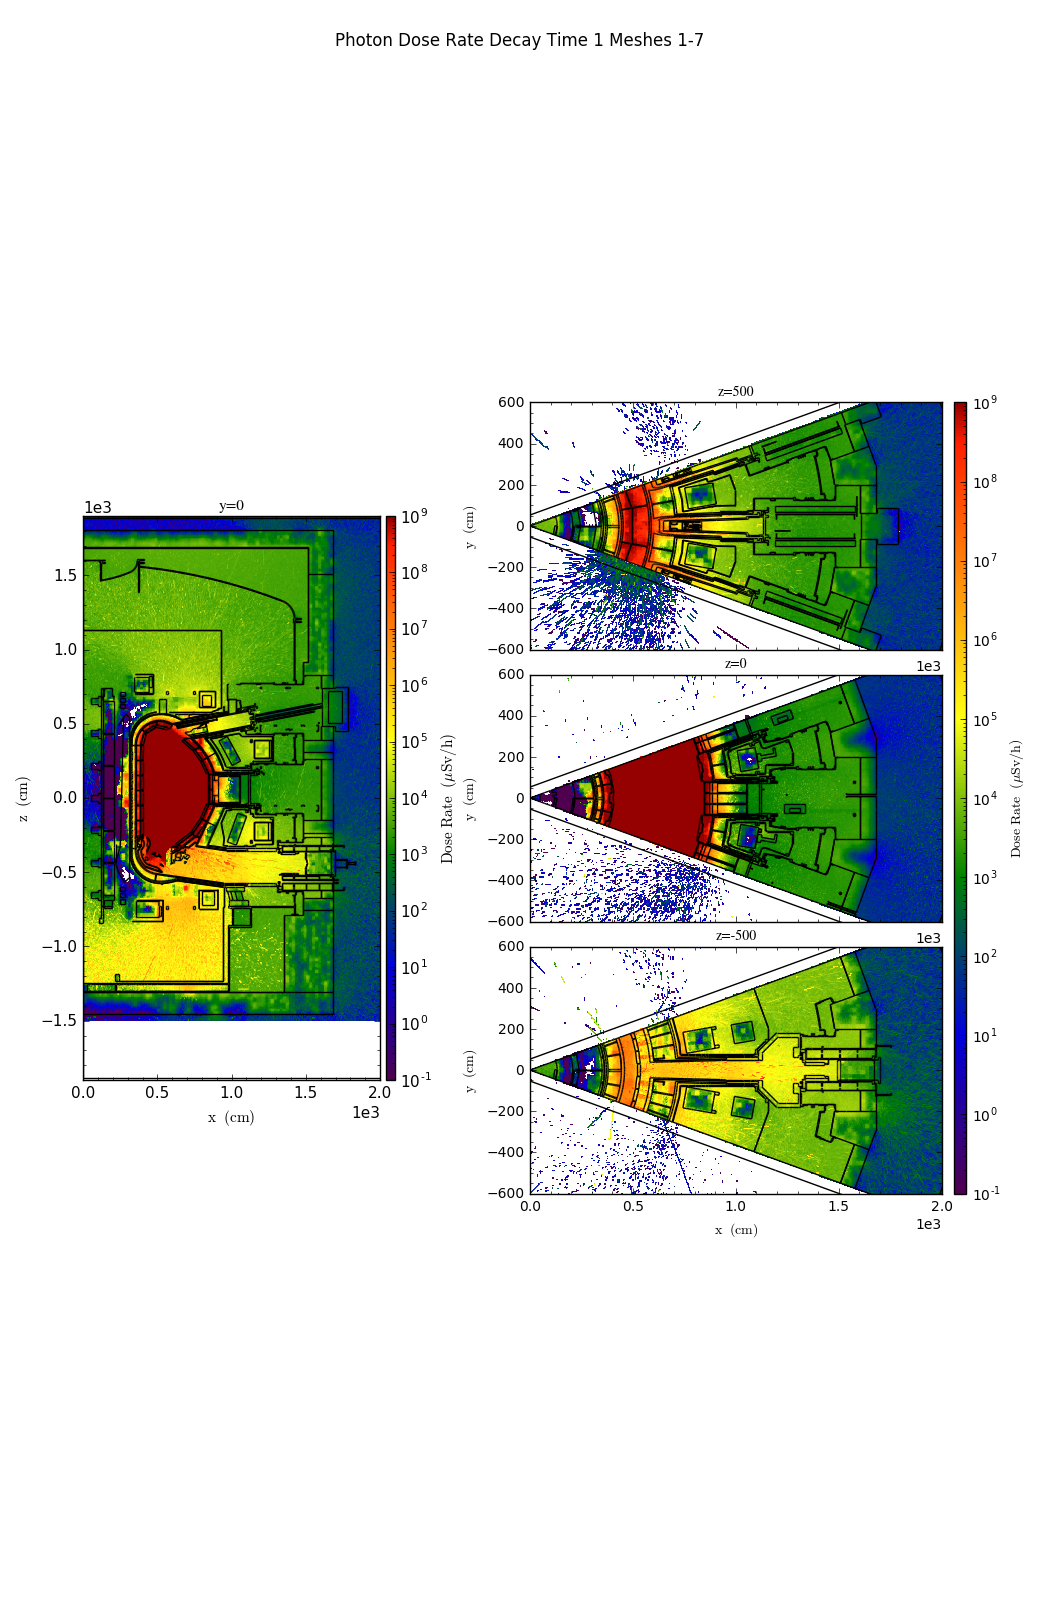
\includegraphics[trim={0cm 9cm 0cm 10cm},clip,scale=0.75]{../plots/final_model_with_b4c/Photon_Dose_Rate_Decay_Time_1_Meshes_1-7.png}
\caption{The total dose rate summed over all meshes for decay time 1}
\label{fig:photons_dc1_b4c_total}
\end{figure}
\begin{figure}[ht!]
\centering
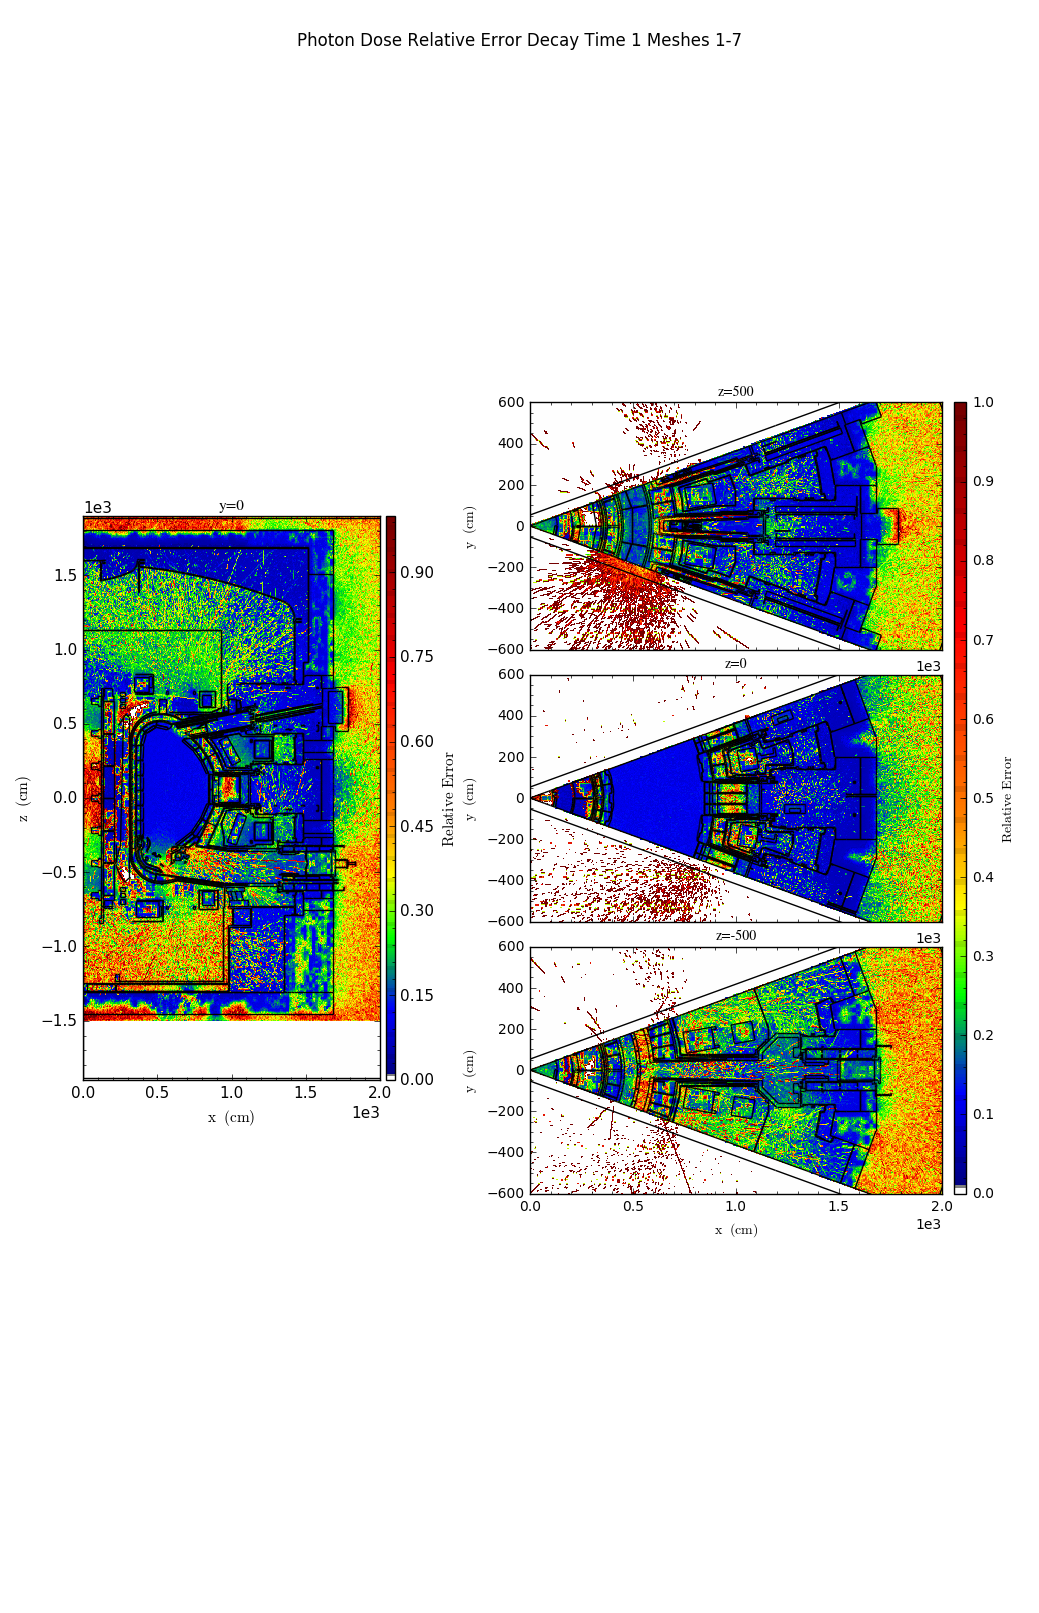
\includegraphics[trim={0cm 9cm 0cm 10cm},clip,scale=0.75]{../plots/final_model_with_b4c/Photon_Dose_Relative_Error_Decay_Time_1_Meshes_1-7.png}
\caption{The error in the total dose rate combined over all meshes for decay time 1}
\label{fig:photons_dc1_b4c_total_error}
\end{figure}
\begin{figure}[ht!]
\centering
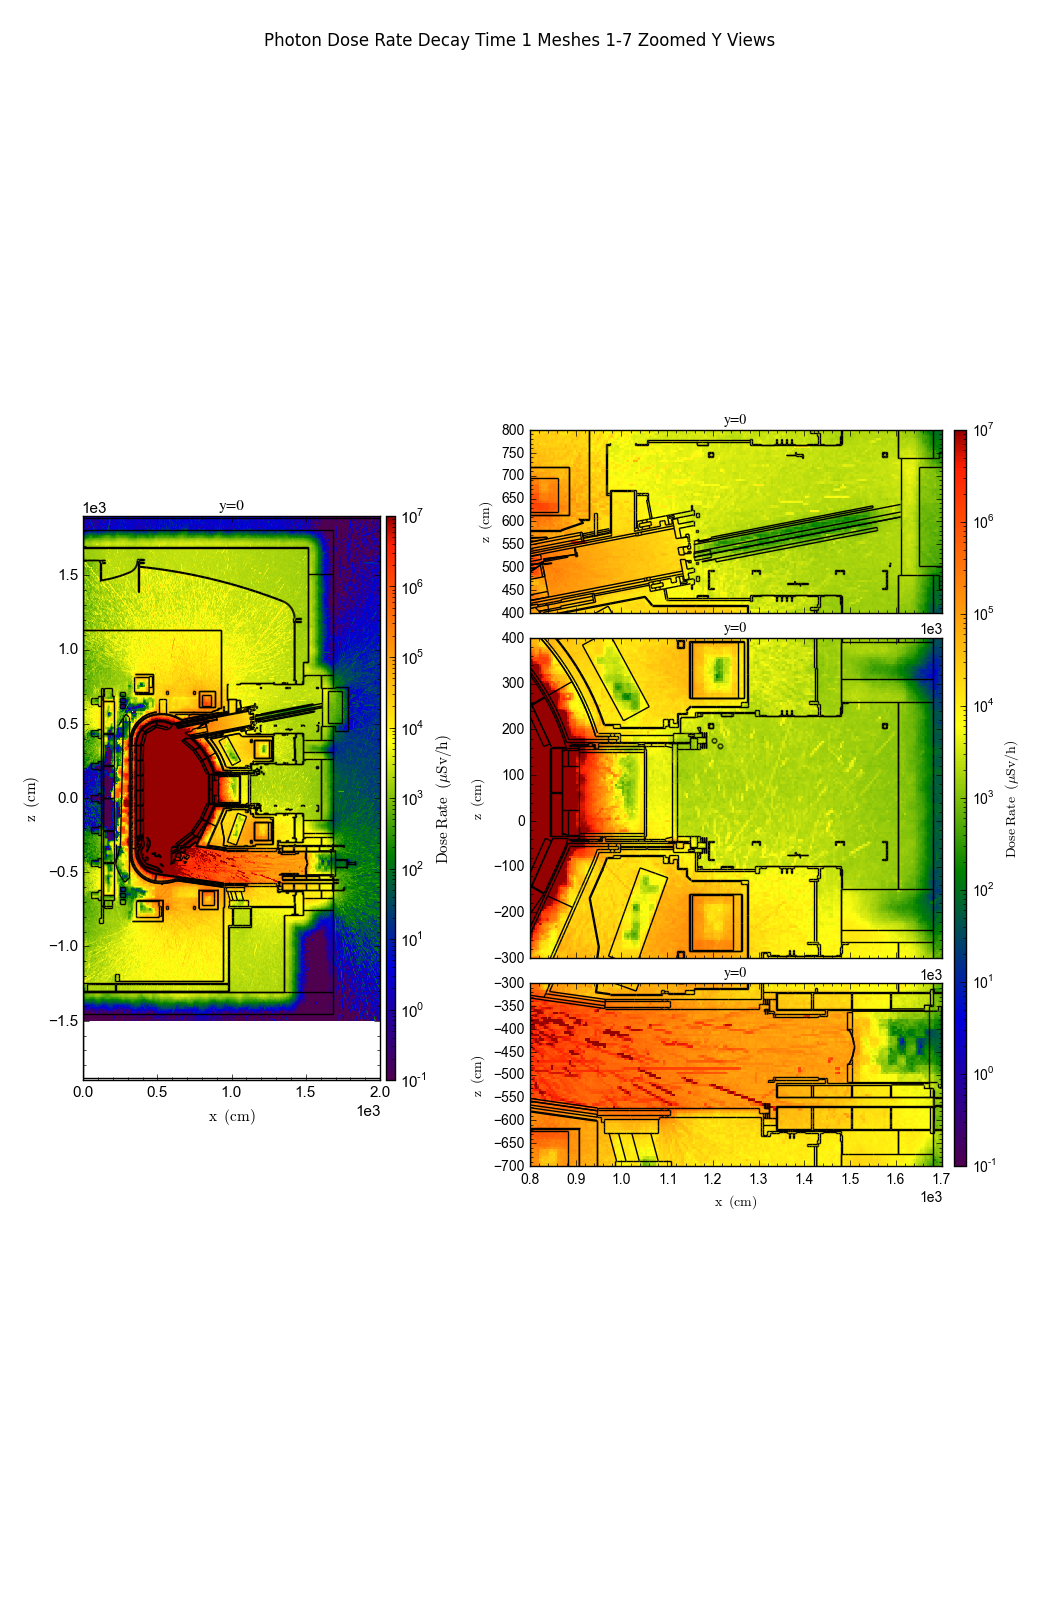
\includegraphics[trim={0cm 9cm 0cm 10cm},clip,scale=0.75]{../plots/final_model_with_b4c/Photon_Dose_Rate_Decay_Time_1_Meshes_1-7_Zoomed_Y_Views.png}
\caption{The total dose rate summed over all meshes for decay time 1, with focus on the port areas}
\label{fig:photons_dc1_b4c_total_zoomed}
\end{figure}
\begin{figure}[ht!]
\centering
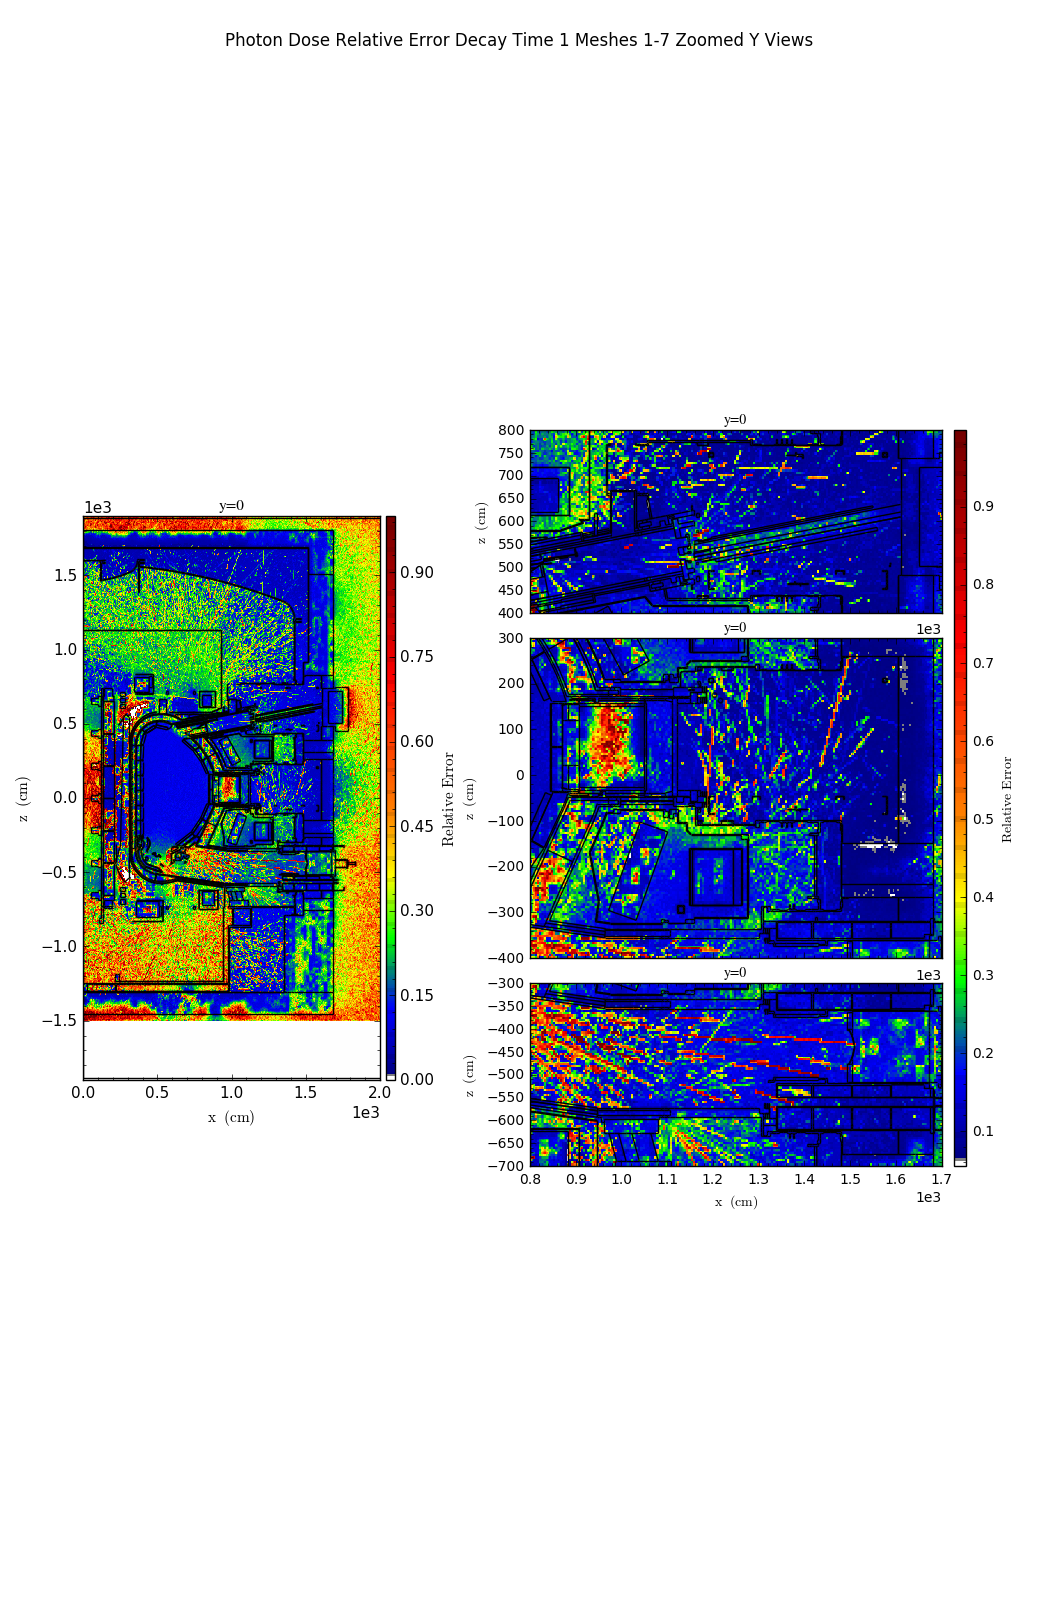
\includegraphics[trim={0cm 9cm 0cm 10cm},clip,scale=0.75]{../plots/final_model_with_b4c/Photon_Dose_Relative_Error_Decay_Time_1_Meshes_1-7_Zoomed_Y_Views.png}
\caption{The error in the total dose rate combined over all meshes for decay time 1, with focus on the port areas}
\label{fig:photons_dc1_b4c_total_error_zoomed}

\end{figure}

\clearpage
\subsubsection{Decay time 2 - $10^6$ s}

%% the totals plots
\begin{figure}[ht!]
\centering
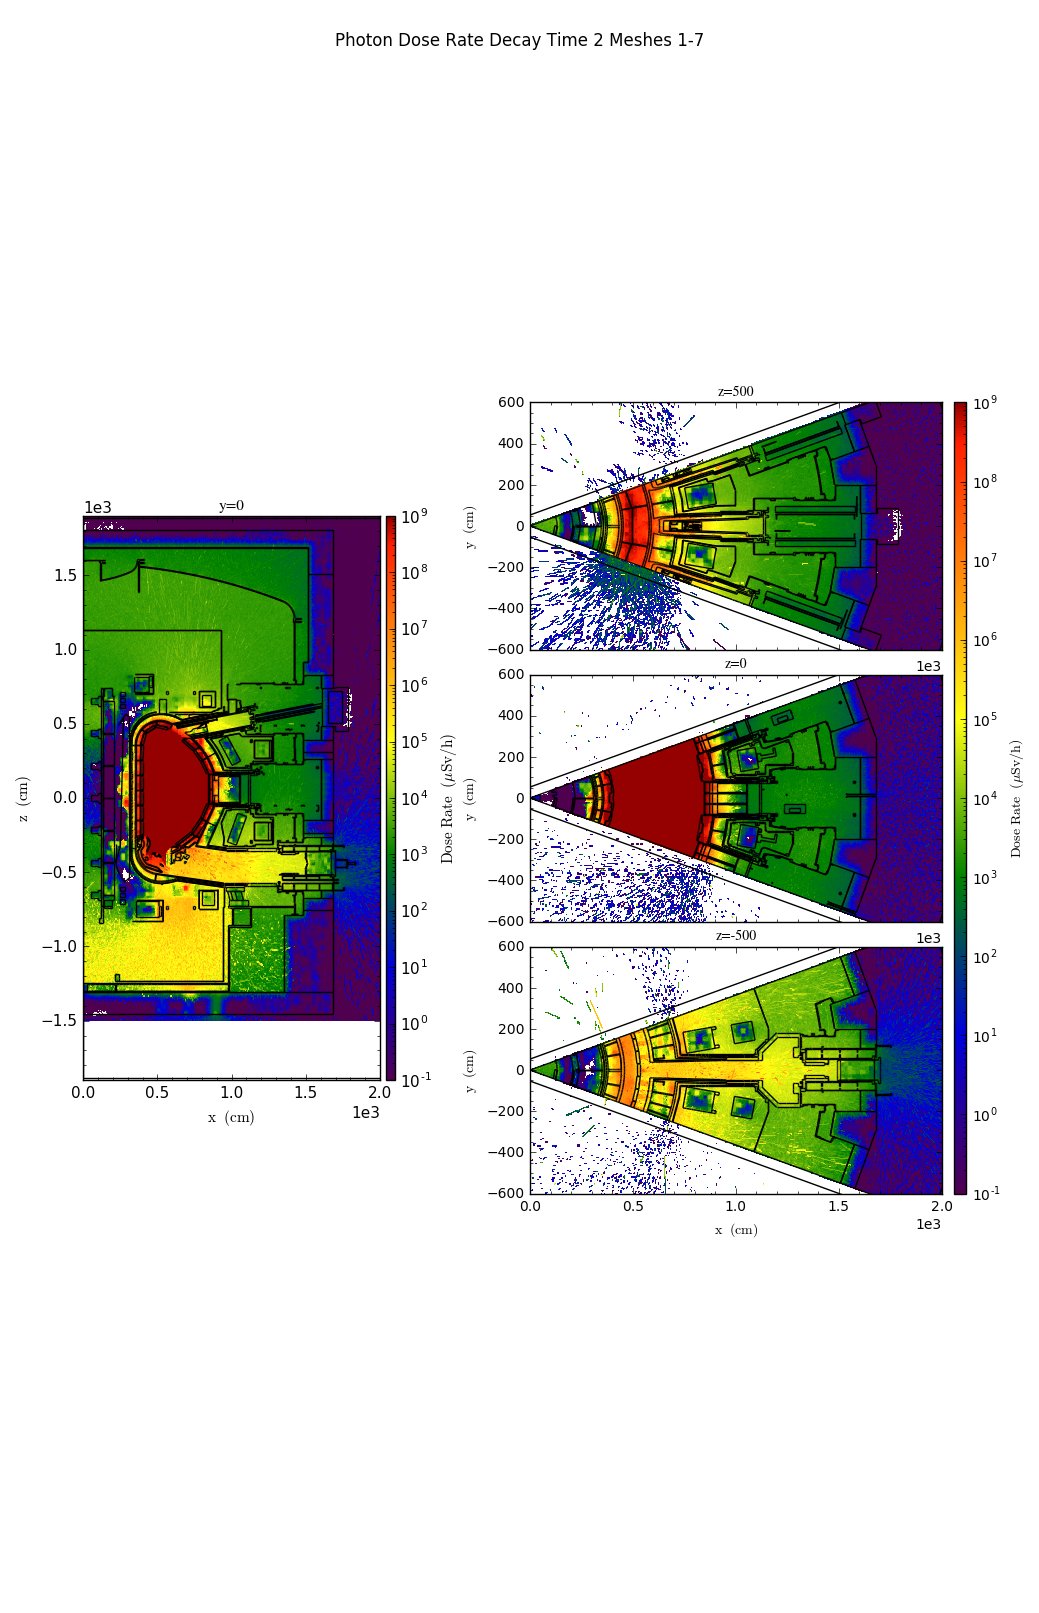
\includegraphics[trim={0cm 9cm 0cm 10cm},clip,scale=0.75]{../plots/final_model_with_b4c/Photon_Dose_Rate_Decay_Time_2_Meshes_1-7.png}
\caption{The total dose rate summed over all meshes for decay time 2}
\label{fig:photons_dc2_b4c_total}
\end{figure}
\begin{figure}[ht!]
\centering
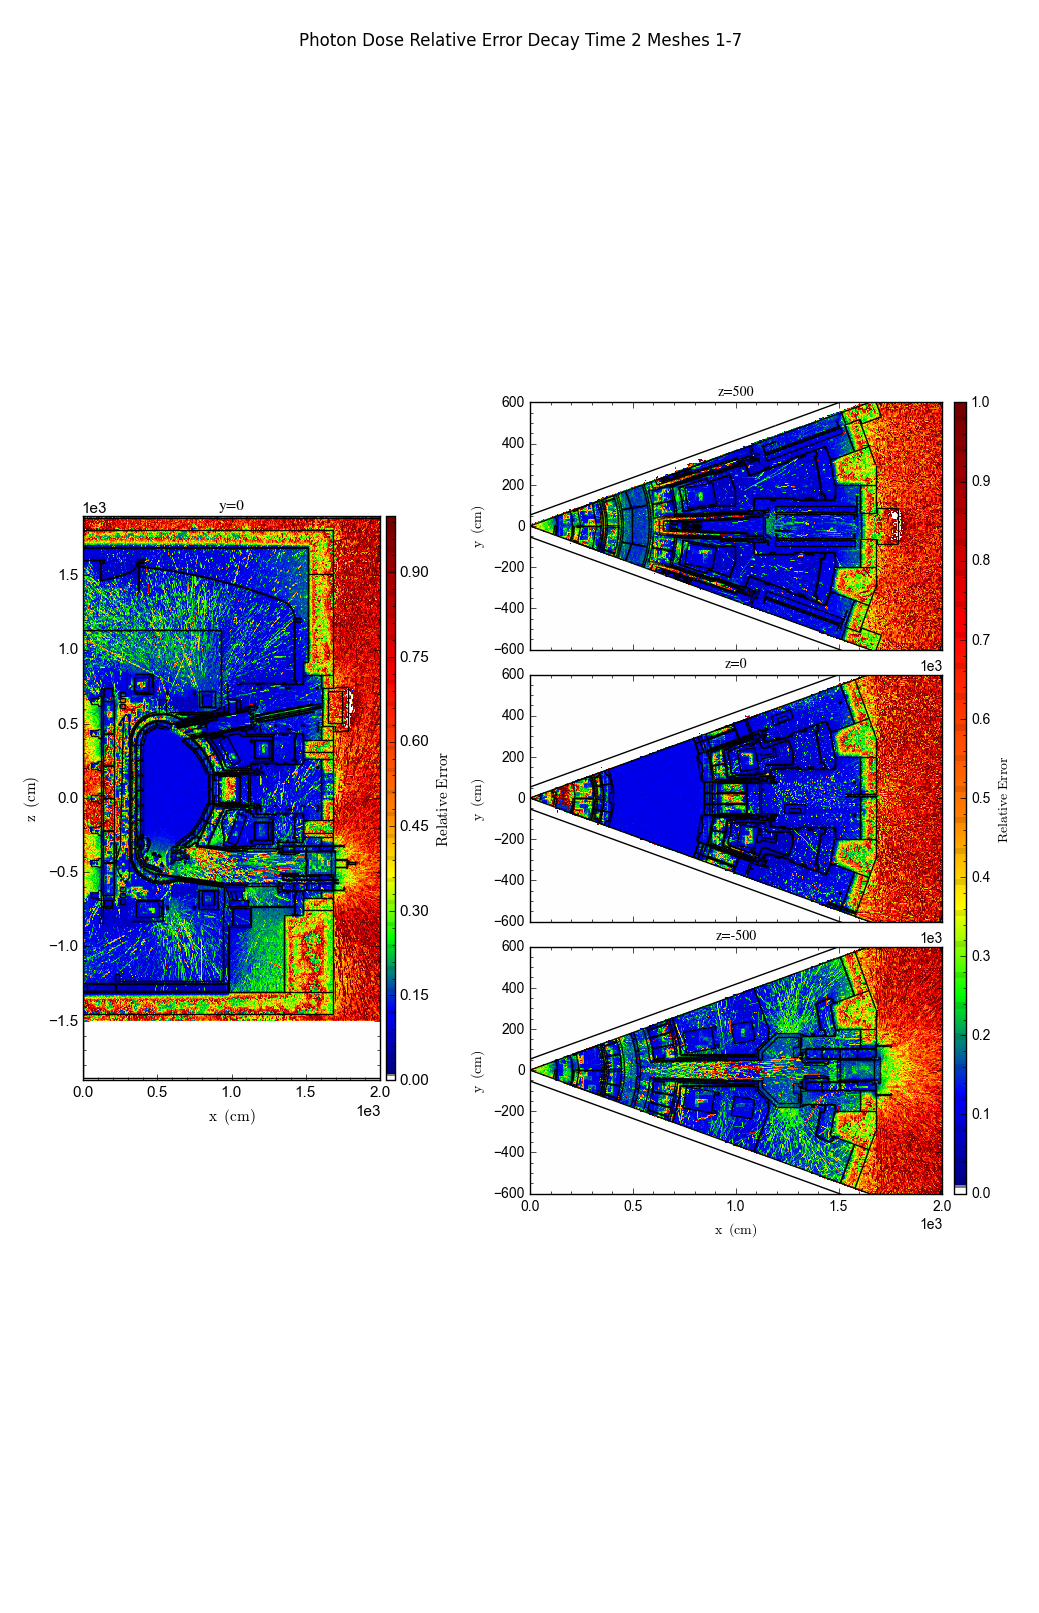
\includegraphics[trim={0cm 9cm 0cm 10cm},clip,scale=0.75]{../plots/final_model_with_b4c/Photon_Dose_Relative_Error_Decay_Time_2_Meshes_1-7.png}
\caption{The error in the total dose rate combined over all meshes for decay time 2}
\label{fig:photons_dc2_b4c_total_error}
\end{figure}
\begin{figure}[ht!]
\centering
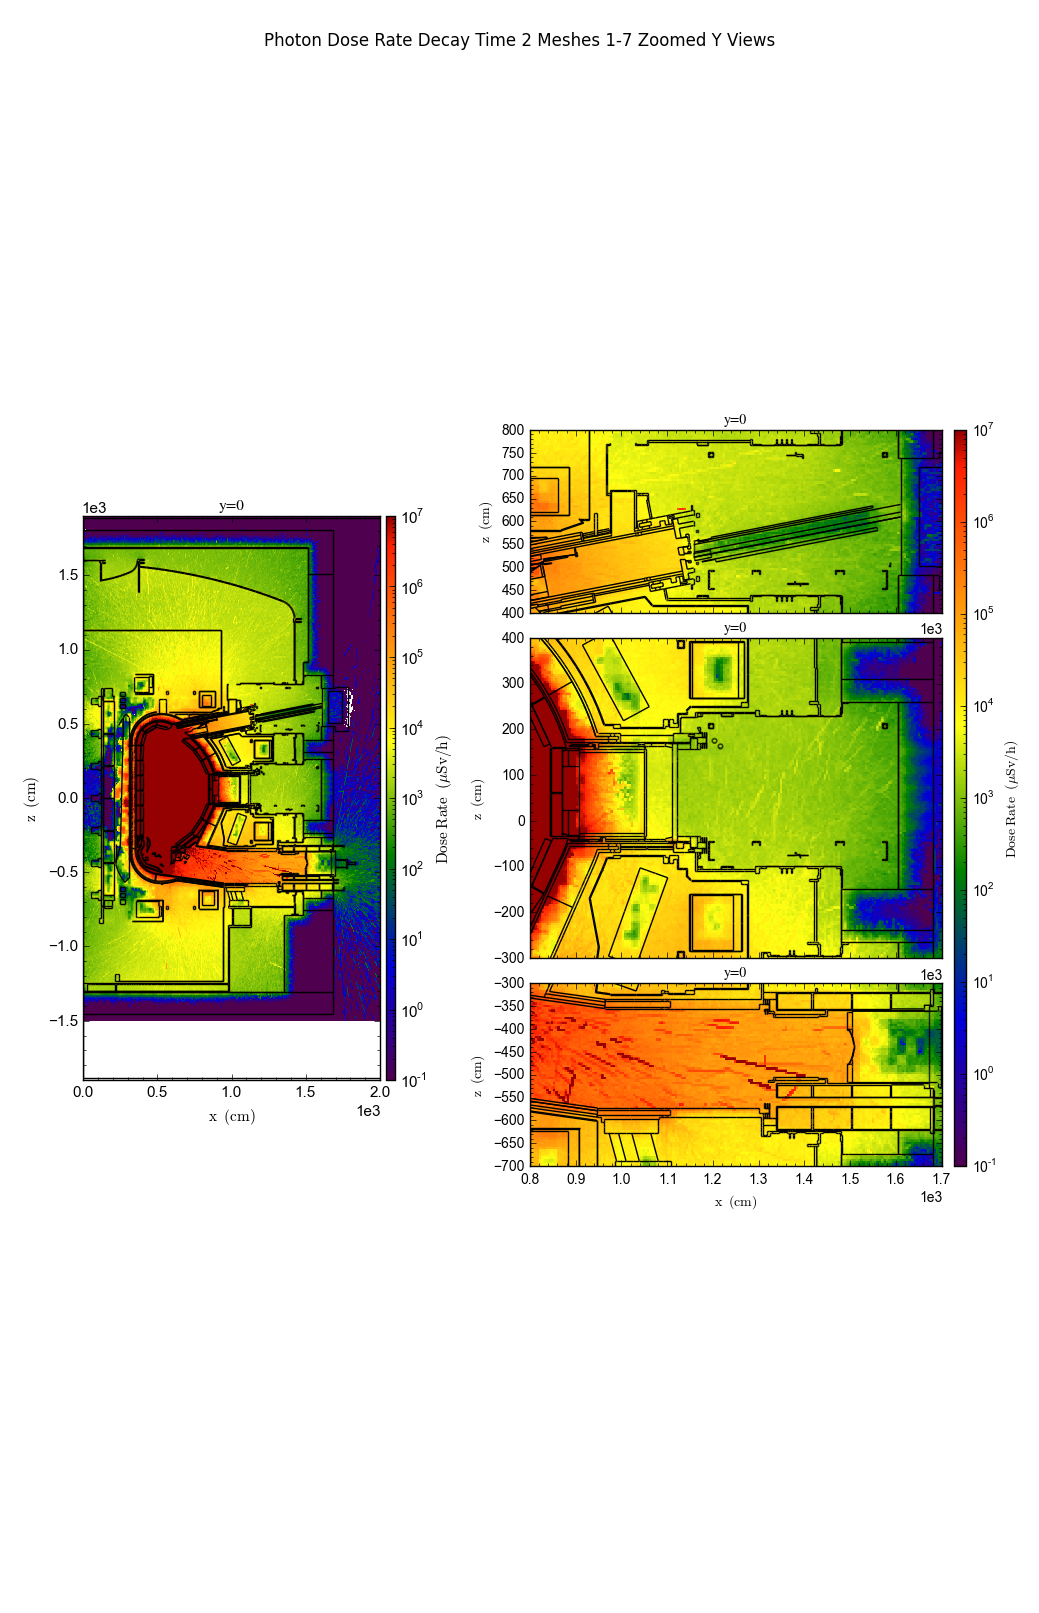
\includegraphics[trim={0cm 9cm 0cm 10cm},clip,scale=0.75]{../plots/final_model_with_b4c/Photon_Dose_Rate_Decay_Time_2_Meshes_1-7_Zoomed_Y_Views.png}
\caption{The total dose rate summed over all meshes for decay time 2, with focus on the port areas}
\label{fig:photons_dc2_b4c_total_zoomed}
\end{figure}
\begin{figure}[ht!]
\centering
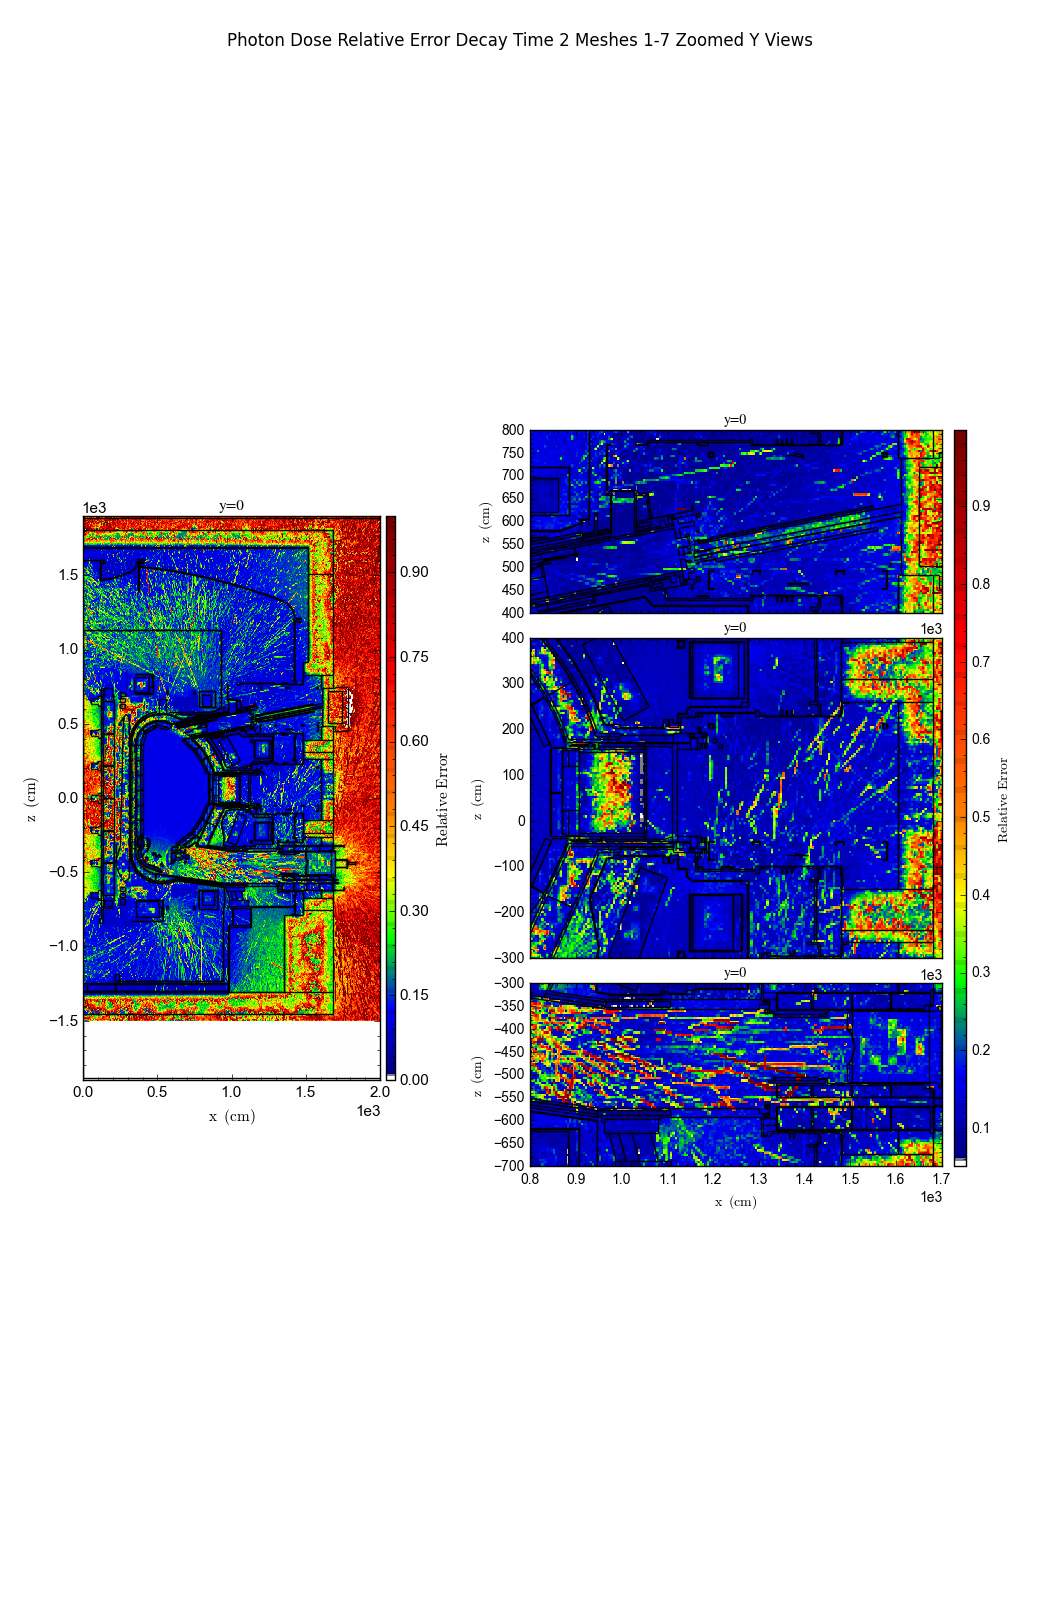
\includegraphics[trim={0cm 9cm 0cm 10cm},clip,scale=0.75]{../plots/final_model_with_b4c/Photon_Dose_Relative_Error_Decay_Time_2_Meshes_1-7_Zoomed_Y_Views.png}
\caption{The error in the total dose rate combined over all meshes for decay time 2, with focus on the port areas}
\label{fig:photons_dc2_b4c_total_error_zoomed}
\end{figure}
\clearpage

\subsubsection{Decay time 3 - $10^7$ s}
%% the totals plots
\begin{figure}[ht!]
\centering
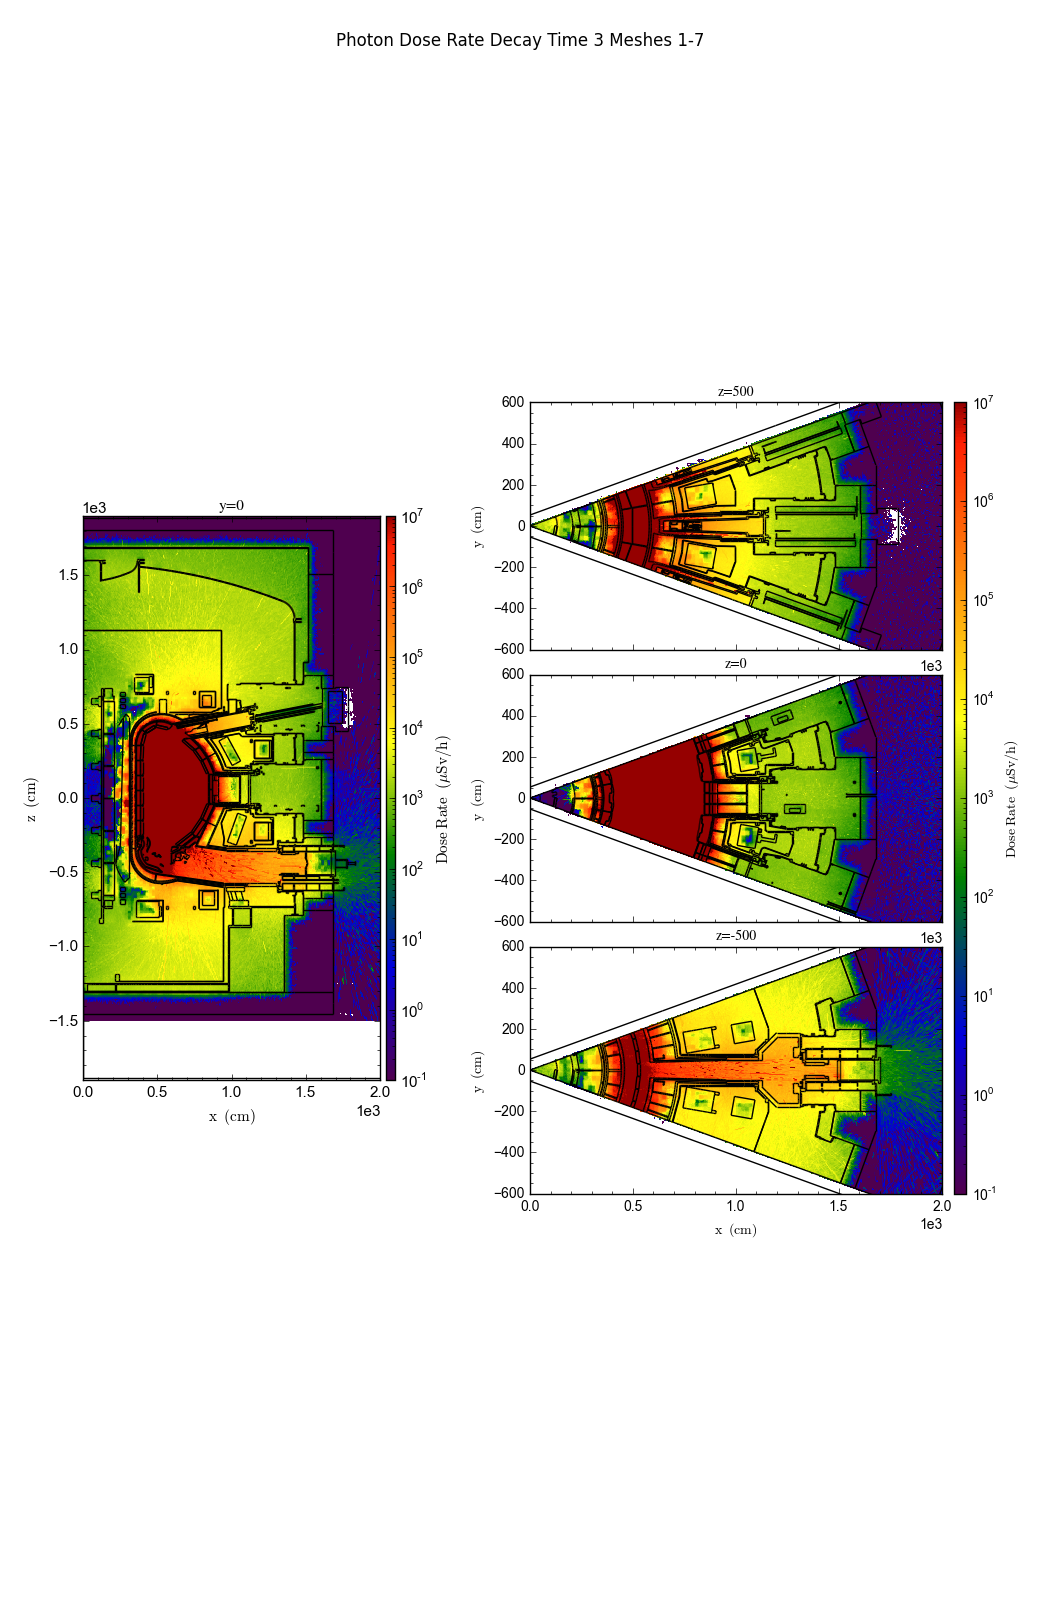
\includegraphics[trim={0cm 9cm 0cm 10cm},clip,scale=0.75]{../plots/final_model_with_b4c/Photon_Dose_Rate_Decay_Time_3_Meshes_1-7.png}
\caption{The total dose rate summed over all meshes for decay time 3}
\label{fig:photons_dc3_b4c_total}
\end{figure}
\begin{figure}[ht!]
\centering
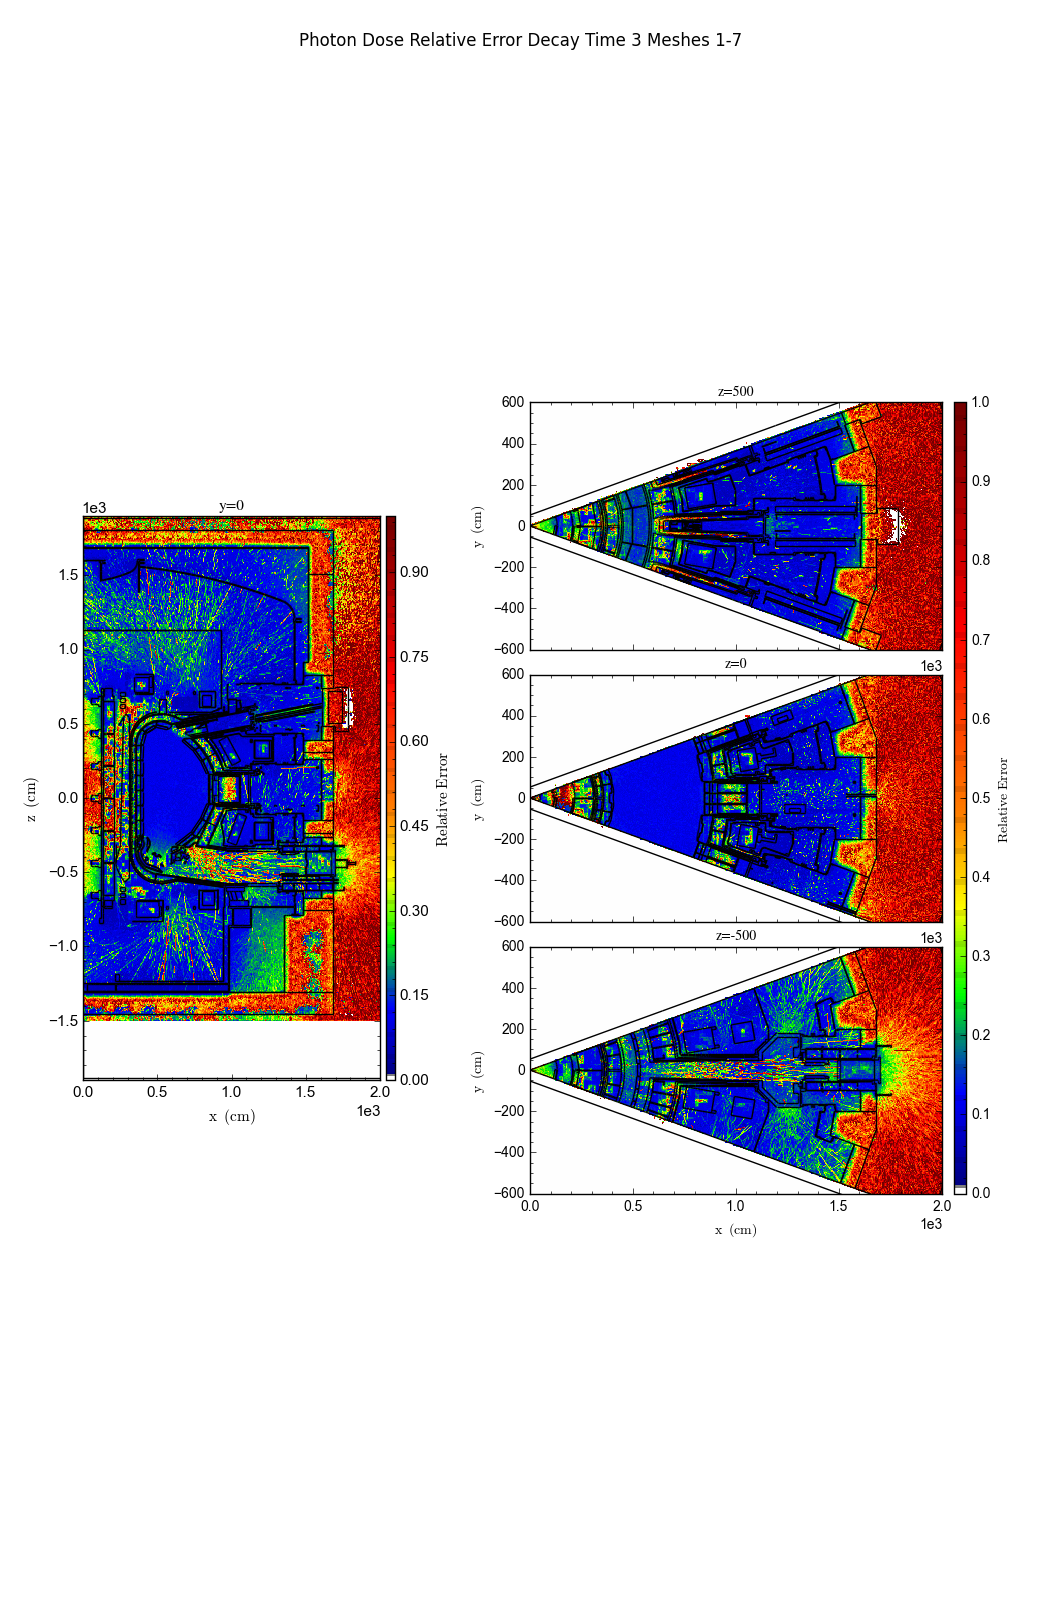
\includegraphics[trim={0cm 9cm 0cm 10cm},clip,scale=0.75]{../plots/final_model_with_b4c/Photon_Dose_Relative_Error_Decay_Time_3_Meshes_1-7.png}
\caption{The error in the total dose rate combined over all meshes for decay time 3}
\label{fig:photons_dc3_b4c_total_error}
\end{figure}
\begin{figure}[ht!]
\centering
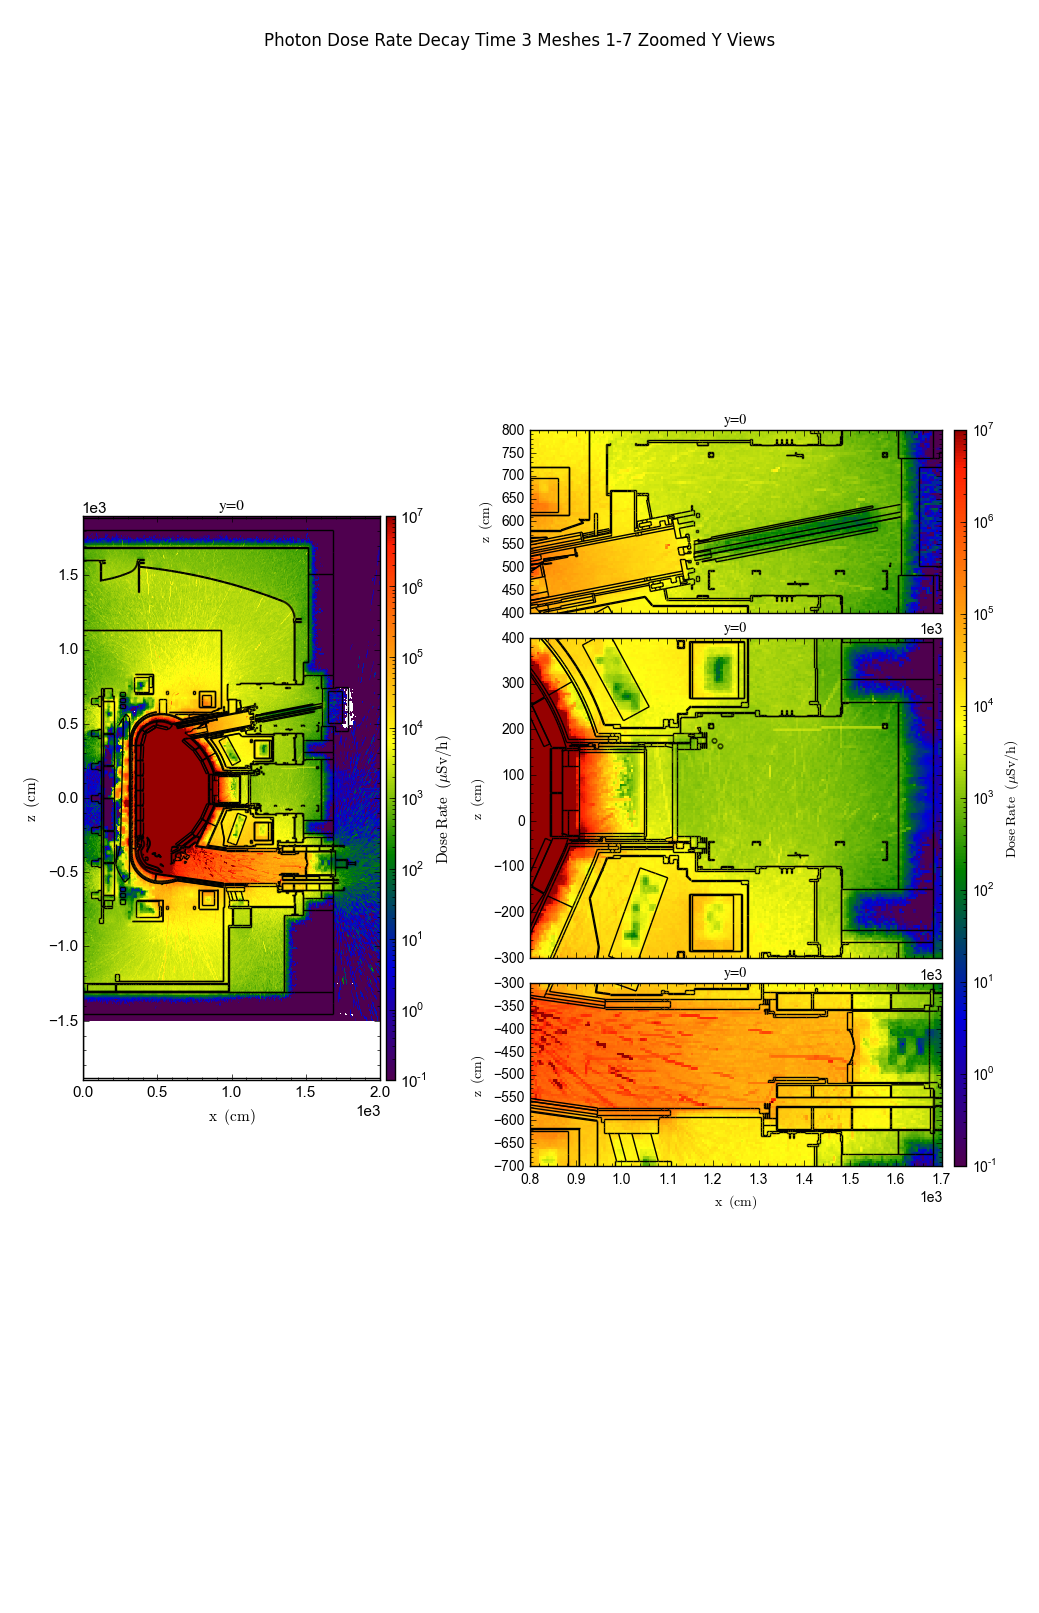
\includegraphics[trim={0cm 9cm 0cm 10cm},clip,scale=0.75]{../plots/final_model_with_b4c/Photon_Dose_Rate_Decay_Time_3_Meshes_1-7_Zoomed_Y_Views.png}
\caption{The total dose rate summed over all meshes for decay time 3, with focus on the port areas}
\label{fig:photons_dc3_b4c_total_zoomed}
\end{figure}
\begin{figure}[ht!]
\centering
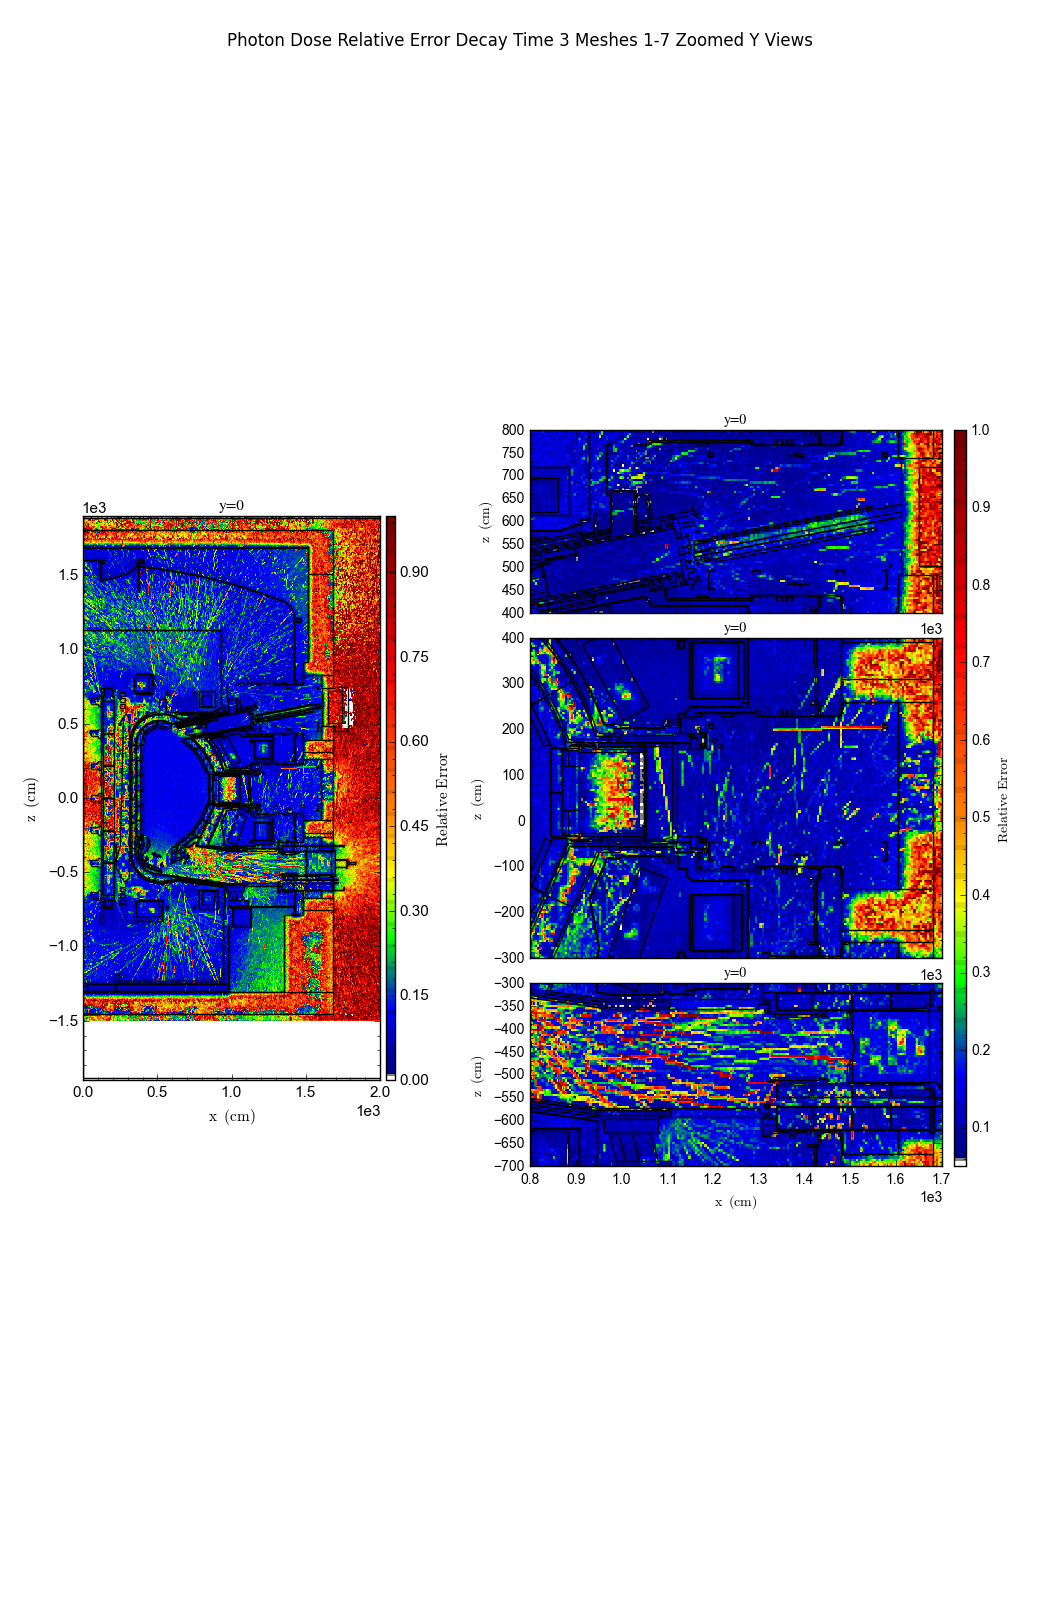
\includegraphics[trim={0cm 9cm 0cm 10cm},clip,scale=0.75]{../plots/final_model_with_b4c/Photon_Dose_Relative_Error_Decay_Time_3_Meshes_1-7_Zoomed_Y_Views.png}
\caption{The error in the total dose rate combined over all meshes for decay time 3, with focus on the port areas}
\label{fig:photons_dc3_b4c_total_error_zoomed}
\end{figure}

%% NOTE [PPHW]: Include line-out plots of total photon dose here and/or ratio
%% - no cross-talk break down yet.  And then also discussion of same....

\newpage
\clearpage
\subsection{Photon Cross Talk}
The impact of decay photons born in areas far from a region of interest and 
streaming to it are known as cross talk. Cross talk makes assigning dose 
budgets to components difficult as there is the possibility that a given 
component will meet its dose budget, but due to leaky adjacent components
may mean that the dose is higher than would otherwise be tolerated. There
have been studies previously done to estimate the degree of cross talk for
a number of ITER \gls{pp} systems, but those calculations were for an older
model with fewer components present in the interspaces. Below are the 
detailed contributions for each mesh shown in Figures 
\ref{fig:ct_photons_dc2_no4bc_m1_flux} to \ref{fig:ct_photons_dc2_no4bc_m7_flux}.

\begin{figure}[ht!]
\centering
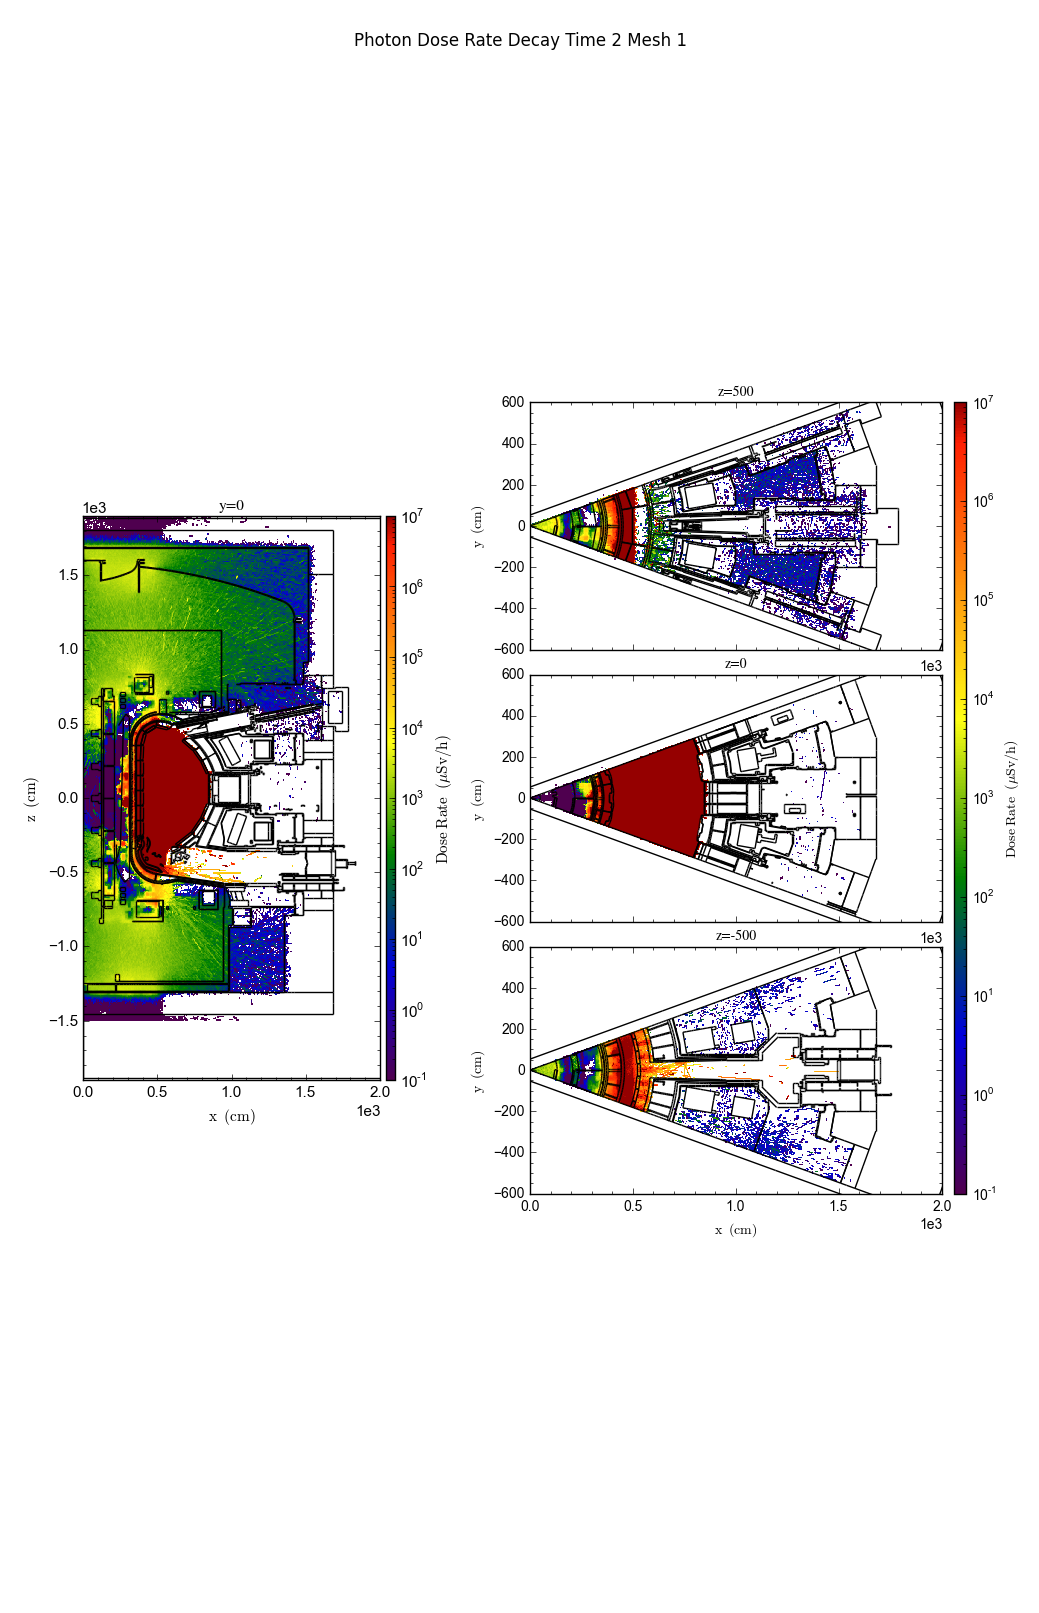
\includegraphics[trim={0cm 9cm 0cm 10cm},clip,scale=0.75]{../plots/final_model/Photon_Dose_Rate_Decay_Time_2_Mesh_1.png}
\caption{The total photon dose from the B$_4$C case for decay time 2 for mesh 1}
\label{fig:ct_photons_dc2_no4bc_m1_flux}
\end{figure}

\newpage
\clearpage

\begin{figure}[ht!]
\centering
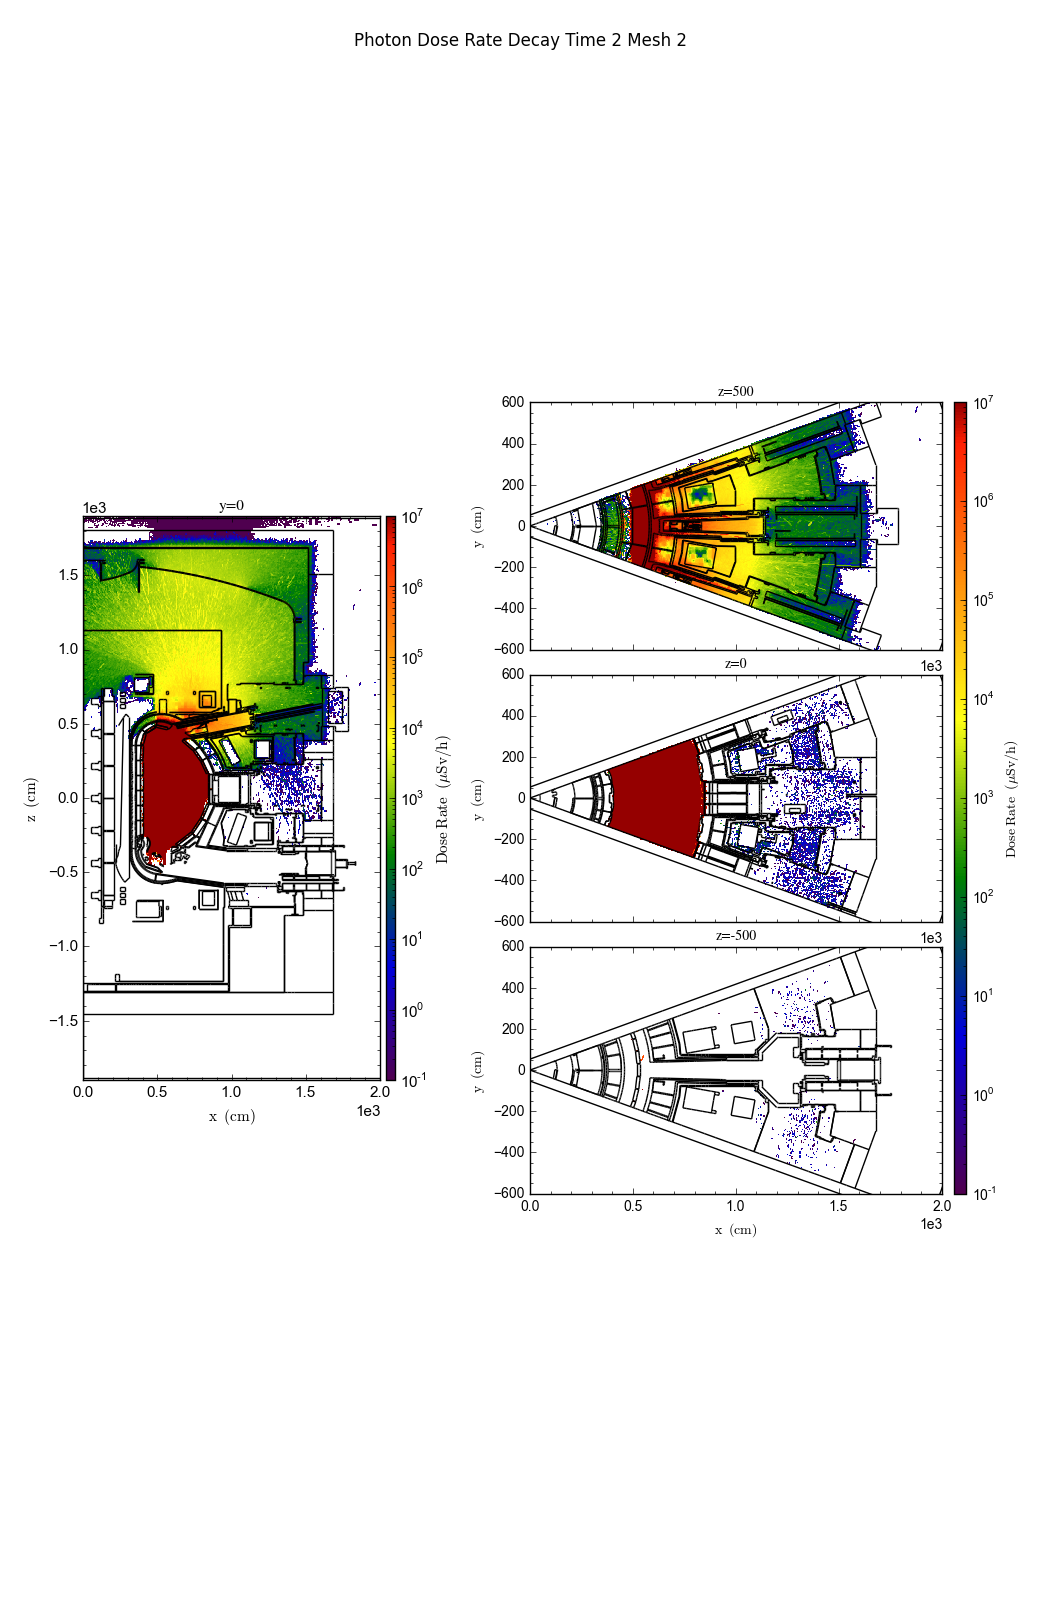
\includegraphics[trim={0cm 9cm 0cm 10cm},clip,scale=0.75]{../plots/final_model/Photon_Dose_Rate_Decay_Time_2_Mesh_2.png}
\caption{The total photon dose from the B$_4$C case for decay time 2 for mesh 2}
\label{fig:ct_photons_dc2_no4bc_m2_flux}
\end{figure}
\newpage
\clearpage

\begin{figure}[ht!]
\centering
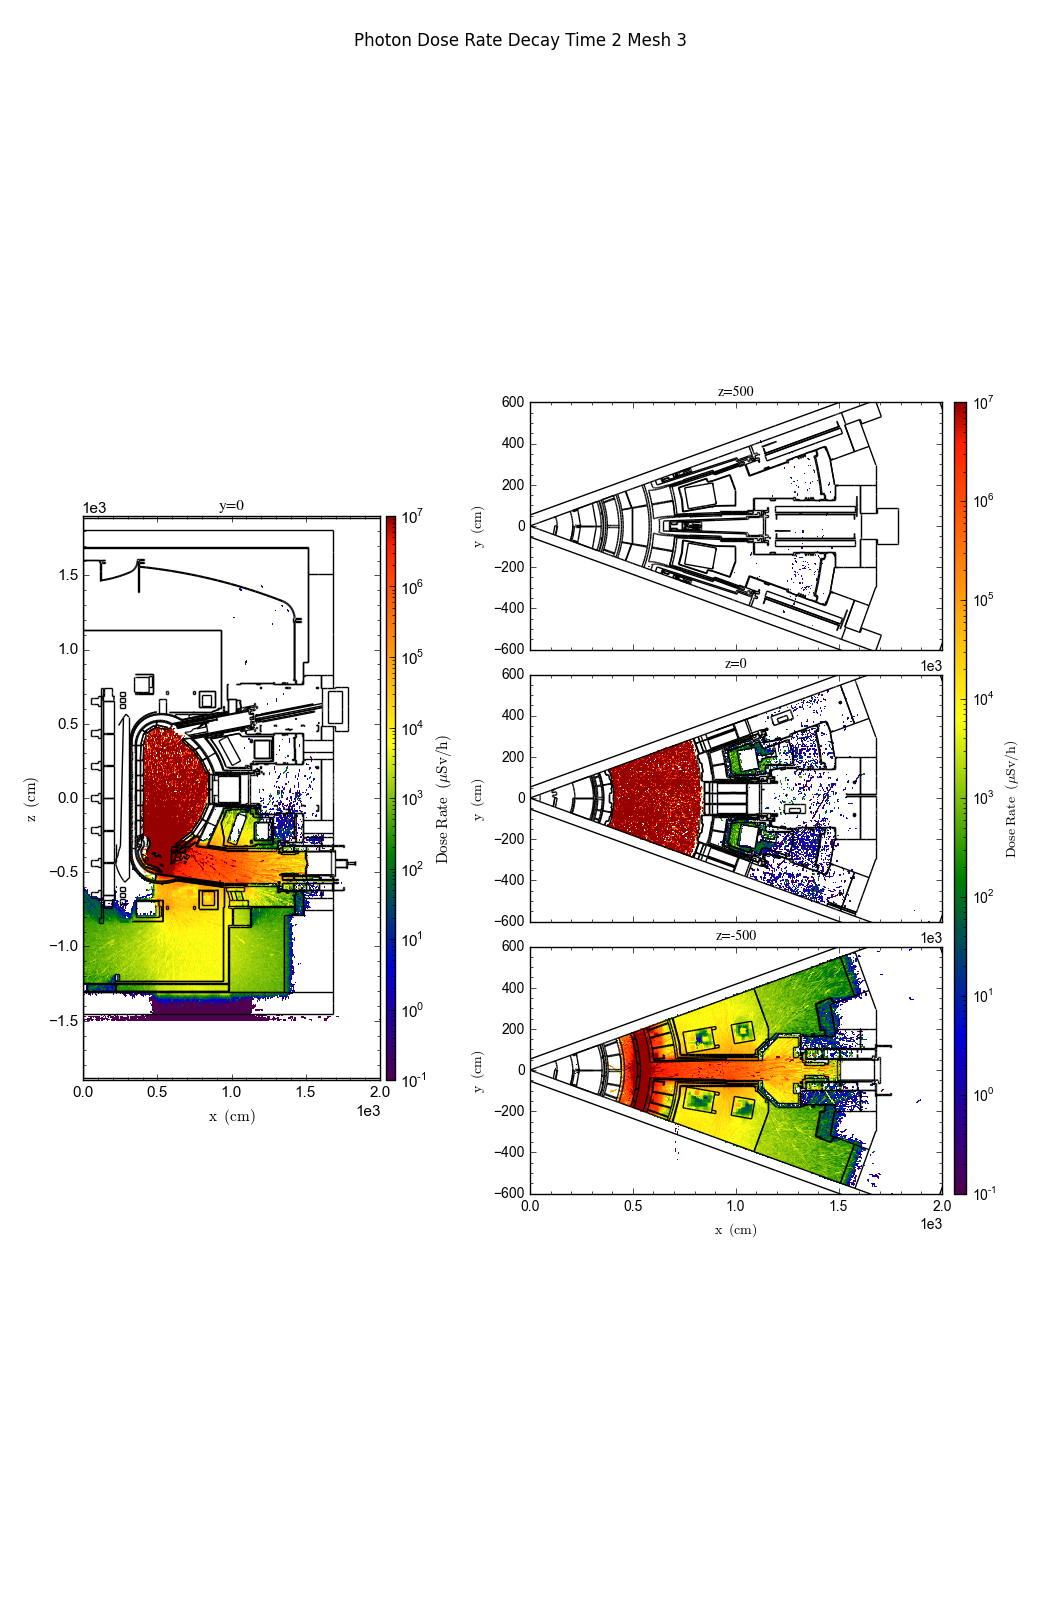
\includegraphics[trim={0cm 9cm 0cm 10cm},clip,scale=0.75]{../plots/final_model/Photon_Dose_Rate_Decay_Time_2_Mesh_3.png}
\caption{The total photon dose from the B$_4$C case for decay time 2 for mesh 3}
\label{fig:ct_photons_dc2_no4bc_m3_flux}
\end{figure}
\newpage
\clearpage

\begin{figure}[ht!]
\centering
\includegraphics[trim={0cm 9cm 0cm 10cm},clip,scale=0.75]{../plots/final_model/Photon_Dose_Rate_Decay_Time_2_Mesh_4.png}
\caption{The total photon dose from the B$_4$C case for decay time 2 for mesh 4}
\label{fig:ct_photons_dc2_no4bc_m4_flux}
\end{figure}
\newpage
\clearpage

\begin{figure}[ht!]
\centering
\includegraphics[trim={0cm 9cm 0cm 10cm},clip,scale=0.75]{../plots/final_model/Photon_Dose_Rate_Decay_Time_2_Mesh_5.png}
\caption{The total photon dose from the B$_4$C case for decay time 2 for mesh 5}
\label{fig:ct_photons_dc2_no4bc_m5_flux}
\end{figure}
\newpage
\clearpage

\begin{figure}[ht!]
\centering
\includegraphics[trim={0cm 9cm 0cm 10cm},clip,scale=0.75]{../plots/final_model/Photon_Dose_Rate_Decay_Time_2_Mesh_6.png}
\caption{The total photon dose from the B$_4$C case for decay time 2 for mesh 6}
\label{fig:ct_photons_dc2_no4bc_m6_flux}
\end{figure}
\newpage
\clearpage

\begin{figure}[ht!]
\centering
\includegraphics[trim={0cm 9cm 0cm 10cm},clip,scale=0.75]{../plots/final_model/Photon_Dose_Rate_Decay_Time_2_Mesh_7.png}
\caption{The total photon dose from the B$_4$C case for decay time 2 for mesh 7}
\label{fig:ct_photons_dc2_no4bc_m7_flux}
\end{figure}

\newpage
\clearpage
\subsubsection{Comparison of total photon doses}
\textbf{placeholder for total photon dose comparison}
\newpage
\clearpage
\subsubsection{Breakdown of Cross Talk}
We can examine the breakdown of cross talk within the problem and the effect 
that the B$_4$C has upon the local fluxes. The full suite of data can be found
in Section \ref{cross_talk_data}, however Figures \ref{fig:ct_ep_dc2},
\ref{fig:ct_ep_dc2_rel}, \ref{fig:b4c_ct_ep_dc2}, and \ref{fig:b4c_ct_ep_dc2_rel} 
show the data for the baseline case and the with B$_4$C case for the equatorial 
port for the second decay times. What is shown in the figures is that the \gls{epi}
region around 70-90\% of the photon dose is produced by local activation, there are
significant contributions from the the upper port in the range 0-10\% and 
similarly 0-30\% of the photon dose originates from the pumping port. The 
addition of the B$_4$C layer does little to alter the distribution of 
relative contribution or the absolute value of SDR.
\\
\\
For the \gls{upp}, the Figures are contained in Section \ref{appendix} and are 
shown in Figures \ref{appendix:pt_ct_base} to \ref{appendix:pt_ct_b4c}. 
Both the baseline case finds the doserate in 
the \gls{upi} is much higher than the 100 $\mu$Sv/hr guideline, just behind the 
\gls{upp} the doserate is more than 1 mSv/hr and even the contribution to the 
dose from the \gls{epi} activation is more than the 100 $\mu$Sv/hr guideline. 
The background contribution from mesh 2, containing activation of the upper
outboard side of ITER also contributes some 80 $\mu$Sv/hr to the dose rate in 
the \gls{epi}.
\\
\\
For the \gls{pp} the Figures are contained in Section \ref{appendix} and are 
shown in Figures \ref{} to \ref{}. Both cases find the doserate in 
the cryopump is significant $\sim$ 100 mSv/hr in the region of the cyropump. 
This simulation contained the unshielded pumping port and thus the doserate is 
very high due to neutrons streaming along the pumping port. 

\begin{figure}[ht!]
\centering
\includegraphics[clip,scale=0.25]{../plots/crosstalk/nob4c/ep/dc2.png}
\caption{Absolute contributions to dose from each mesh, considering a line along, 
         0,0,0 along the x direction for the 2nd decay time - baseline case}
\label{fig:ct_ep_dc2}
\end{figure}
\begin{figure}[ht!]
\centering
\includegraphics[clip,scale=0.25]{../plots/crosstalk/nob4c/ep/dc2_rel.png}
\caption{Relative contributions to dose from each mesh, considering a line along, 
         0,0,0 along the x direction for the 2nd decay time - baseline case}
\label{fig:ct_ep_dc2_rel}
\end{figure}

\begin{figure}[ht!]
\centering
\includegraphics[clip,scale=0.25]{../plots/crosstalk/b4c/ep/dc2.png}
\caption{Absolute contributions to dose from each mesh, considering a line along,
         0,0,0 along the x direction for the 2nd decay time - with B$_4$C}
\label{fig:b4c_ct_ep_dc2}
\end{figure}
\begin{figure}[ht!]
\centering
\includegraphics[clip,scale=0.25]{../plots/crosstalk/b4c/ep/dc2_rel.png}
\caption{Relative contributions to dose from each mesh, considering a line along, 
         0,0,0 along the x direction for the 2nd decay time - with B$_4$C }
\label{fig:b4c_ct_ep_dc2_rel}
\end{figure}

\newpage
\clearpage
\subsection{Conclusion}
It is clear from Figures \ref{fig:photons_dc1_no4bc_total} to 
\ref{fig:photons_dc3_b4c_total_error_zoomed} that the shutdown photon dose rate 
in the port interspace is slightly affected by the addition of boron carbide 
to the plasma side surface of the bioshield. The reason for the this is 
significantly degraded thermal flux which impacts the importance of (n,$\gamma$)
 reactions and also the transport of neutrons back from the bioshield. The true 
benefit appears only to be very close to the B$_4$C layer, where it reduces the
activation of steel components near to the bioshield, those components away
from the bioshield appear to have their activation dominated by the neutron
transported via long paths around other ports. This is  likely due to the fact
that most neutron induced activation in fusion devices are due to high energy
capture reactions like (n,p), (n,2n) and (n,xn) reactions.
\\
\\
What is clear is that the shutdown photon dose rate at the second decay time is
significantly higher than the desired target goal of 100 $\mu$Sv hr$^{-1}$,
previous analysis has shown ranges of \gls{sdr} in the \gls{epi} of anywhere
from 200 to 400 $\mu$Sv hr$^{-1}$. It is surmised that the reason for the
significantly higher \gls{sdr} in this calculation is due to the increased
mass of components modelled in the \gls{epi} which leads to higher \gls{sdr}.
The \gls{pfc}3 \& 4 coils also are strong sources near the \gls{epi}, but being
beyond the \gls{ve} are somewhat shielded by it. The \gls{bs} is als a
significant source, unshielded due to is proximity to the \gls{epi}. The ever
present photon cross talk is also present, the \gls{lp} being unplugged leads
to strong sources in the cryopump, which has roughly the same contribution
as the sources within the \gls{epi}.
\\
\\
The individual cross talk contributions from meshes 5,6 and 7 (pumping duct, 
upper port and equatorial port respectively) is in each case over the 100 
$\mu$Sv/hr threshold, i.e. the cross talk from mesh 6 to mesh 5 is more than 100 
$\mu$Sv/hr, similarly for mesh 5 to 7 etc. The worst example of cross talk was 
found to be excessive streaming 
\\
\\
It is also apparent that the utility of the B$_4$C present in the \gls{gepp}
design is not as high as may be imagined. The B$_4$C powder is contained within
a stainless steel lined box, which itself becomes activated under the presence
of neutrons. The largest components in the region which do become activated are
the back plate and attachment flange, both of which are the dominant source of
activation in the region. It is suggested that the front 50 cm of the B$_4$C
drawers could be removed, reducing the weight of the port plug without
significantly impacting the shielding capability.

%\newpage
%\clearpage
%\section{Acceptance Criteria}

\newpage
\clearpage
\section{Lessons learned and future work}
\subsection*{CAD}
One of the biggest reasons for delay with the deliver of the calculation results
in this task was the cleaning and preparation of the CAD geometry. Several
months were expended cleaning, repairing and merging components together into a
final model. Ultimately due to time contraints, the decision was taken to
proceed with the analysis with the CAD in its current state. It is important
for CAD based workflows to have access to the unmodified, unsimplified CAD
models that have been used to prepare the IO geometries. A specific issue
was the use of the IO supplied Clite CAD geometry which was unprepared for
such an analysis, several stages of simplification and fixing has been performed
which lead to problems downstream in the final CAD preparation.

\subsection*{High Throughput Methodology}
The splitting of a given \gls{mcnp5} calculation into subruns spanning the same random
number space proved to be a successful way of performing these calculations with
access to the large of amounts of CPU-time on \gls{uw}'s \gls{chtc} system. In
the future, we expect to make increasing use of this method for MCNP
calculations. In this specific case long histories were a pervasive problem and
limited the total number of runs that could be completed, however the underlying
method was reliable. One of the issues associated with such a method is the
quantity of storage space required to store the intermediate split results prior
to merging, in this batch of simulations a total sum of 1.8 Tb of data was
produced, consider that this represents only 10\% of the completed runs,
therefore this simulation should have consumed some 20 Tb of space.

\subsection*{Variance Reduction}
The neutron section of this work was impacted by long histories, which appear to
be a pervasive problem in the ITER geometry due to the area available for
neutrons to stream through, combined with the strong neutron attenuation though
bulk shielding. Ultimately this problem needs a solution and there are several
potential solutions but each must be appropriately weighed and considered to
ensure that a fair game is being played when rouletting particles. A future
work could be to investigate several potential solutions to the ``long history
problem'' and then provide recommendations to IO.
\\
\\
The authors will also like to note that the use of use of global MC 
variance-reduction techniques, including the FW-CADIS method does not 
provide optimum variance reduction parameters for SDR calculations. 
The goal of these global MC variance-reduction techniques is to uniformly 
distribute the Monte Carlo computational efforts throughout numerous 
phase-space segments to calculate many Monte Carlo tallies with nearly 
uniform relative uncertainties. Even though SDR analysis requires the 
calculation of space- and energy-dependent neutron fluxes, the goal of 
the analysis is the accurate assessment of the final \gls{sdr}. Global 
Monte Carlo variance-reduction techniques do not focus MC computational 
efforts on calculating the production rates of radioisotopes that will 
ultimately contribute to the \gls{sdr}. On the contrary, the Multi-Step 
Consistent Adjoint Driven Importance Sampling (MS-CADIS) hybrid 
MC/deterministic method is currently under development to speed up the \gls{sdr}
 Monte Carlo neutron transport calculation using an importance function that 
represents the neutron importance to the final \gls{sdr} \cite{mscadis}. 
The MS-CADIS method uses the CADIS method to develop consistent source biasing 
and weight window variance-reduction parameters. However, because the MS-CADIS 
method focuses on multistep shielding calculations such as the \gls{r2s} 
calculations of \gls{sdr}, it develops an importance function for the initial 
radiation transport calculation (e.g., the neutron calculations in \gls{sdr} 
simulations) that represents the importance of particles to the final response
 of the overall simulation. Reference \ref{mscadis} explains the theory of the MS-CADIS 
method and provides some insights into the physical interpretations of the 
MS-CADIS adjoint neutron source and the MS-CADIS adjoint neutron flux.

\newpage
\clearpage
\bibliographystyle{unsrt}
\bibliography{bibliography}
\newpage
\clearpage
\section{Appendix - A - Materials used in the problem}
\begin{centering}
\begin{longtable}[ht!]
{ p{0.3\textwidth} | p{0.3\textwidth} }
\hline
Element \& Mass Fraction\\
\hline
H &  6.998686e-04\\
B &  9.937634e-06\\
C &  2.946747e-04\\
N &  6.956582e-04\\
O &  5.539577e-03\\
Si &  4.968734e-03\\
P &  2.484376e-04\\
S &  9.937764e-05\\
Ti &  9.934530e-04\\
Cr &  1.739088e-01\\
Mn &  1.788766e-02\\
Fe &  6.443977e-01\\
Co &  4.968802e-04\\
Ni &  1.217351e-01\\
Cu &  2.981281e-03\\
Nb &  9.937617e-05\\
Mo &  2.484404e-02\\
Ta &  9.937573e-05\\
\caption{Table showing the elemental description of material M942}
\label{table:material_EPP3L}
\end{longtable}
\clearpage
\begin{longtable}[ht!]
  { p{0.3\textwidth} | p{0.3\textwidth} }
\hline
Element \& Mass Fraction\\
\hline
He &  3.355146e-03\\
B &  9.781345e-04\\
C &  1.970612e-04\\
N &  9.196549e-04\\
O &  1.378506e-02\\
Al &  6.199031e-04\\
Si &  1.410760e-02\\
P &  2.955888e-04\\
S &  1.970642e-04\\
K &  7.614452e-05\\
Ti &  1.383993e-03\\
V &  2.627356e-05\\
Cr &  1.136640e-01\\
Mn &  1.313740e-02\\
Fe &  4.264464e-01\\
Co &  3.284351e-04\\
Ni &  7.882409e-02\\
Cu &  2.771454e-01\\
Zr &  1.313594e-05\\
Nb &  2.401275e-02\\
Mo &  1.642176e-02\\
Sn &  7.995497e-03\\
Ta &  6.052439e-03\\
W &  6.568622e-06\\
Pb &  5.254980e-06\\
Bi &  5.254959e-06\\
\caption{Table showing the elemental description of material M908}
\label{table:material_M908}
\end{longtable}
\clearpage
\begin{longtable}[ht!]
  { p{0.3\textwidth} | p{0.3\textwidth} }
\hline
Element \& Mass Fraction\\
\hline
B &  1.800292e-05\\
C &  3.000486e-04\\
N &  1.100178e-03\\
Si &  1.000162e-02\\
P &  3.000486e-04\\
S &  1.500243e-04\\
Ti &  1.000162e-03\\
Cr &  2.000324e-01\\
Mn &  2.000324e-02\\
Fe &  6.399737e-01\\
Co &  1.000162e-03\\
Ni &  1.200194e-01\\
Nb &  1.000162e-03\\
Mo &  5.000810e-03\\
Ta &  1.000162e-04\\
\caption{Table showing the elemental description of material M917}
\label{table:material_CryoPipes}
\end{longtable}
\clearpage

\begin{longtable}[ht!]
  { p{0.3\textwidth} | p{0.3\textwidth} }
\hline
Element \& Mass Fraction\\
\hline
H &  5.005935e-06\\
C &  2.968774e-05\\
N &  1.001227e-05\\
O &  2.995422e-05\\
Na &  1.001186e-05\\
Mg &  5.005930e-06\\
Al &  1.501778e-05\\
Si &  2.002347e-05\\
P &  5.005883e-05\\
S &  5.006025e-06\\
K &  1.001096e-05\\
Ca &  1.001235e-05\\
Ti &  1.000875e-05\\
Cr &  1.001193e-05\\
Mn &  5.005959e-06\\
Fe &  3.003566e-05\\
Co &  1.001190e-05\\
Ni &  2.002367e-05\\
Cu &  1.001186e-05\\
Zr &  1.001074e-05\\
Nb &  1.001189e-05\\
Mo &  1.001187e-04\\
Ta &  1.001185e-05\\
W &  9.995651e-01\\
Pb &  9.873957e-06\\
\caption{Table showing the elemental description of material M74}
\label{table:material_M74}
\end{longtable}
\clearpage

\begin{longtable}[ht!]
{ p{0.3\textwidth} | p{0.3\textwidth} }
\hline
Element \& Mass Fraction\\
\hline
B &  1.000003e-05\\
C &  2.965249e-04\\
N &  7.000261e-04\\
Si &  4.999931e-03\\
P &  2.499975e-04\\
S &  1.000016e-04\\
Ti &  9.996906e-04\\
Cr &  1.750007e-01\\
Mn &  1.799997e-02\\
Fe &  6.484436e-01\\
Co &  4.999999e-04\\
Ni &  1.224995e-01\\
Cu &  2.999999e-03\\
Nb &  1.000001e-04\\
Mo &  2.500003e-02\\
Ta &  9.999969e-05\\
\caption{Table showing the elemental description of material M913}
\label{table:material_EppDucts}
\end{longtable}
\clearpage
\begin{longtable}[ht!]
{ p{0.3\textwidth} | p{0.3\textwidth} }
\hline
Element \& Mass Fraction\\
\hline
H &  6.386261e-04\\
He &  3.220044e-03\\
B &  6.262540e-06\\
C &  6.839086e-03\\
N &  1.721870e-03\\
O &  1.269236e-02\\
Mg &  8.473257e-04\\
Al &  3.419589e-03\\
Si &  1.128000e-02\\
P &  2.818109e-04\\
S &  6.669566e-04\\
K &  3.130979e-06\\
Ti &  1.204138e-02\\
V &  2.504891e-05\\
Cr &  1.064636e-01\\
Mn &  1.252507e-02\\
Fe &  4.065706e-01\\
Co &  3.131276e-04\\
Ni &  7.915245e-02\\
Cu &  3.072425e-01\\
Zr &  1.252369e-05\\
Nb &  1.828886e-02\\
Mo &  1.565635e-02\\
Sn &  1.252512e-05\\
Ta &  6.262504e-05\\
W &  6.262465e-06\\
Pb &  5.010050e-06\\
Bi &  5.010036e-06\\
\caption{Table showing the elemental description of material M906}
\label{table:material_M906}
\end{longtable}
\clearpage
\begin{longtable}[ht!]
{ p{0.3\textwidth} | p{0.3\textwidth} }
\hline
Element \& Mass Fraction\\
\hline
He &  3.098619e-03\\
B &  9.218565e-04\\
C &  2.047632e-04\\
N &  9.555961e-04\\
O &  1.298416e-02\\
Al &  6.157792e-04\\
Si &  1.376589e-02\\
P &  3.071415e-04\\
S &  2.047662e-04\\
K &  7.203318e-05\\
Ti &  1.392027e-03\\
V &  2.730040e-05\\
Cr &  1.178762e-01\\
Mn &  1.365088e-02\\
Fe &  4.431132e-01\\
Co &  3.412721e-04\\
Ni &  8.190491e-02\\
Cu &  2.562974e-01\\
Zr &  1.364937e-05\\
Nb &  2.218681e-02\\
Mo &  1.706357e-02\\
Sn &  7.386505e-03\\
Ta &  5.597890e-03\\
W &  6.825360e-06\\
Pb &  5.460369e-06\\
Bi &  5.460353e-06\\
\caption{Table showing the elemental description of material M907}
\label{table:material_M907}
\end{longtable}
\clearpage
\begin{longtable}[ht!]
{ p{0.3\textwidth} | p{0.3\textwidth} }
\hline
Element \& Mass Fraction\\
\hline
H &  4.123240e-04\\
B &  9.963269e-06\\
C &  2.954349e-04\\
N &  6.974529e-04\\
O &  3.263613e-03\\
Si &  4.981552e-03\\
P &  2.490785e-04\\
S &  9.963397e-05\\
Ti &  9.960158e-04\\
Cr &  1.743574e-01\\
Mn &  1.793380e-02\\
Fe &  6.460600e-01\\
Co &  4.981619e-04\\
Ni &  1.220492e-01\\
Cu &  2.988971e-03\\
Nb &  9.963253e-05\\
Mo &  2.490813e-02\\
Ta &  9.963210e-05\\
\caption{Table showing the elemental description of material M934}
\label{table:material_UPDSM}
\end{longtable}
\clearpage
\begin{longtable}[ht!]
{ p{0.3\textwidth} | p{0.3\textwidth} }
\hline
Element \& Mass Fraction\\
\hline
B &  1.000003e-05\\
C &  2.965249e-04\\
N &  7.000261e-04\\
Si &  4.999931e-03\\
P &  2.499975e-04\\
S &  1.000016e-04\\
Ti &  9.996906e-04\\
Cr &  1.750007e-01\\
Mn &  1.799997e-02\\
Fe &  6.484436e-01\\
Co &  4.999999e-04\\
Ni &  1.224995e-01\\
Cu &  2.999999e-03\\
Nb &  1.000001e-04\\
Mo &  2.500003e-02\\
Ta &  9.999969e-05\\
\caption{Table showing the elemental description of material M933}
\label{table:material_EPTRAP}
\end{longtable}
\clearpage
\begin{longtable}[ht!]
{ p{0.3\textwidth} | p{0.3\textwidth} }
\hline
Element \& Mass Fraction\\
\hline
B &  1.000003e-05\\
C &  2.965249e-04\\
N &  7.000261e-04\\
Si &  4.999931e-03\\
P &  2.499975e-04\\
S &  1.000016e-04\\
Ti &  9.996906e-04\\
Cr &  1.750007e-01\\
Mn &  1.799997e-02\\
Fe &  6.484436e-01\\
Co &  4.999999e-04\\
Ni &  1.224995e-01\\
Cu &  2.999999e-03\\
Nb &  1.000001e-04\\
Mo &  2.500003e-02\\
Ta &  9.999969e-05\\
\caption{Table showing the elemental description of material M929}
\label{table:material_PPWater}
\end{longtable}
\clearpage
\begin{longtable}[ht!]
  { p{0.3\textwidth} | p{0.3\textwidth} }
\hline
Element \& Mass Fraction\\
\hline
Al &  9.749971e-02\\
Si &  1.999971e-03\\
Mn &  9.999996e-03\\
Fe &  4.000005e-02\\
Co &  5.000005e-04\\
Ni &  4.999980e-02\\
Cu &  7.973032e-01\\
Nb &  9.999996e-04\\
Sn &  1.000003e-03\\
Ta &  4.999996e-04\\
Pb &  1.972446e-04\\

\caption{Table showing the elemental description of material M303}
\label{table:material_M303}
\end{longtable}
\clearpage
\begin{longtable}[ht!]
{ p{0.3\textwidth} | p{0.3\textwidth} }
\hline
Element \& Mass Fraction\\
\hline
B &  1.000011e-04\\
C &  7.907392e-04\\
Al &  3.500018e-03\\
Si &  9.999944e-03\\
P &  3.999987e-04\\
S &  3.000072e-04\\
Ti &  2.124361e-02\\
V &  2.999879e-03\\
Cr &  1.475017e-01\\
Mn &  2.000011e-02\\
Fe &  5.221630e-01\\
Co &  2.000021e-03\\
Ni &  2.550009e-01\\
Nb &  1.000009e-03\\
Mo &  1.250011e-02\\
Ta &  5.000035e-04\\
\caption{Table showing the elemental description of material 946}
\label{table:material_EPPCH}
\end{longtable}
\clearpage

\begin{longtable}[ht!]
{ p{0.3\textwidth} | p{0.3\textwidth} }
\hline
Element \& Mass Fraction\\
\hline
B &  7.826302e-01\\
C &  2.173698e-01\\
\caption{Table showing the elemental description of material 910}
\label{table:material_B4C}
\end{longtable}
\clearpage

\begin{longtable}[ht!]
{ p{0.3\textwidth} | p{0.3\textwidth} }
\hline
Element \& Mass Fraction\\
\hline
H &  1.847593e-03\\
B &  1.052615e-05\\
C &  2.246913e-04\\
N &  6.614350e-04\\
O &  1.468420e-02\\
Al &  5.622494e-04\\
Si &  4.789446e-03\\
P &  2.389155e-04\\
S &  7.355948e-05\\
K &  4.723997e-06\\
Ti &  1.578480e-03\\
V &  3.778995e-05\\
Cr &  1.689219e-01\\
Mn &  1.707051e-02\\
Fe &  6.167665e-01\\
Co &  5.028159e-04\\
Ni &  1.251771e-01\\
Cu &  2.148775e-02\\
Zr &  4.164644e-05\\
Nb &  1.010637e-03\\
Mo &  2.416070e-02\\
Sn &  1.890806e-05\\
Ta &  1.034368e-04\\
W &  9.458099e-06\\
Pb &  7.431736e-06\\
Bi &  7.547778e-06\\
\caption{Table showing the elemental description of material M936}
\label{table:material_ShieldBlock}
\end{longtable}
\clearpage

\begin{longtable}[ht!]
{ p{0.3\textwidth} | p{0.3\textwidth} }
\hline
Element \& Mass Fraction\\
\hline
B &  1.000003e-05\\
C &  2.965249e-04\\
N &  7.000261e-04\\
Si &  4.999931e-03\\
P &  2.499975e-04\\
S &  1.000016e-04\\
Ti &  9.996906e-04\\
Cr &  1.750007e-01\\
Mn &  1.799997e-02\\
Fe &  6.484436e-01\\
Co &  4.999999e-04\\
Ni &  1.224995e-01\\
Cu &  2.999999e-03\\
Nb &  1.000001e-04\\
Mo &  2.500003e-02\\
Ta &  9.999969e-05\\
\caption{Table showing the elemental description of material M914}
\label{table:material_UppDucts}
\end{longtable}
\clearpage

\begin{longtable}[ht!]
  { p{0.3\textwidth} | p{0.3\textwidth} }
\hline
Element \& Mass Fraction\\
\hline
H &  5.557512e-03\\
O &  4.968034e-01\\
Na &  1.710308e-02\\
Mg &  2.563458e-03\\
Al &  4.697334e-02\\
Si &  3.151305e-01\\
S &  1.281754e-03\\
K &  1.924422e-02\\
Ca &  8.294590e-02\\
Fe &  1.239677e-02\\
\caption{Table showing the elemental description of material M200}
\label{table:material_M200}
\end{longtable}
\clearpage

\begin{longtable}[ht!]
{ p{0.3\textwidth} | p{0.3\textwidth} }
\hline
Element \& Mass Fraction\\
\hline
B &  1.000003e-05\\
C &  2.965249e-04\\
N &  7.000261e-04\\
Si &  4.999931e-03\\
P &  2.499975e-04\\
S &  1.000016e-04\\
Ti &  9.996906e-04\\
Cr &  1.750007e-01\\
Mn &  1.799997e-02\\
Fe &  6.484436e-01\\
Co &  4.999999e-04\\
Ni &  1.224995e-01\\
Cu &  2.999999e-03\\
Nb &  1.000001e-04\\
Mo &  2.500003e-02\\
Ta &  9.999969e-05\\
\caption{Table showing the elemental description of material M924}
\label{table:material_EppDiagPipes}
\end{longtable}

\begin{longtable}[ht!]
{ p{0.3\textwidth} | p{0.3\textwidth} }
\hline
Element \& Mass Fraction\\
\hline
B &  1.000003e-05\\
C &  2.965249e-04\\
N &  7.000261e-04\\
Si &  4.999931e-03\\
P &  2.499975e-04\\
S &  1.000016e-04\\
Ti &  9.996906e-04\\
Cr &  1.750007e-01\\
Mn &  1.799997e-02\\
Fe &  6.484436e-01\\
Co &  4.999999e-04\\
Ni &  1.224995e-01\\
Cu &  2.999999e-03\\
Nb &  1.000001e-04\\
Mo &  2.500003e-02\\
Ta &  9.999969e-05\\
\caption{Table showing the elemental description of material M939}
\label{table:material_EppWaterPipes}
\end{longtable}
\clearpage

\begin{longtable}[ht!]
{ p{0.3\textwidth} | p{0.3\textwidth} }
\hline
Element \& Mass Fraction\\
\hline
B &  1.000003e-05\\
C &  2.965249e-04\\
N &  7.000261e-04\\
Si &  4.999931e-03\\
P &  2.499975e-04\\
S &  1.000016e-04\\
Ti &  9.996906e-04\\
Cr &  1.750007e-01\\
Mn &  1.799997e-02\\
Fe &  6.484436e-01\\
Co &  4.999999e-04\\
Ni &  1.224995e-01\\
Cu &  2.999999e-03\\
Nb &  1.000001e-04\\
Mo &  2.500003e-02\\
Ta &  9.999969e-05\\
\caption{Table showing the elemental description of material M920}
\label{table:material_EppDIagBox}
\end{longtable}
\clearpage

\begin{longtable}[ht!]
{ p{0.3\textwidth} | p{0.3\textwidth} }
\hline
Element \& Mass Fraction\\
\hline
H &  5.455781e-03\\
B &  9.513635e-06\\
C &  2.821022e-04\\
N &  6.659774e-04\\
O &  4.318342e-02\\
Si &  4.756739e-03\\
P &  2.378378e-04\\
S &  9.513758e-05\\
Ti &  9.510665e-04\\
Cr &  1.664888e-01\\
Mn &  1.712447e-02\\
Fe &  6.169039e-01\\
Co &  4.756803e-04\\
Ni &  1.165412e-01\\
Cu &  2.854081e-03\\
Nb &  9.513620e-05\\
Mo &  2.378404e-02\\
Ta &  9.513578e-05\\
\caption{Table showing the elemental description of material M931}
\label{table:material_UPDFW2}
\end{longtable}
\clearpage

\begin{longtable}[ht!]
{ p{0.3\textwidth} | p{0.3\textwidth} }
\hline
Element \& Mass Fraction\\
\hline
B &  1.000003e-05\\
C &  2.965249e-04\\
N &  7.000261e-04\\
Si &  4.999931e-03\\
P &  2.499975e-04\\
S &  1.000016e-04\\
Ti &  9.996906e-04\\
Cr &  1.750007e-01\\
Mn &  1.799997e-02\\
Fe &  6.484436e-01\\
Co &  4.999999e-04\\
Ni &  1.224995e-01\\
Cu &  2.999999e-03\\
Nb &  1.000001e-04\\
Mo &  2.500003e-02\\
Ta &  9.999969e-05\\
\caption{Table showing the elemental description of material M927}
\label{table:material_PPWheelsDrives}
\end{longtable}
\clearpage

\begin{longtable}[ht!]
  { p{0.3\textwidth} | p{0.3\textwidth} }
\hline
Element \& Mass Fraction\\
\hline
Mg &  2.420331e-01\\
Al &  1.932231e-01\\
Si &  1.613554e-01\\
Ti &  3.025413e-02\\
Cr &  7.059298e-02\\
Mn &  3.025413e-02\\
Fe &  1.411860e-01\\
Cu &  8.067769e-02\\
Zn &  5.042356e-02\\
\caption{Table showing the elemental description of material M912}
\label{table:material_UppExFrames}
\end{longtable}
\clearpage

\begin{longtable}[ht!]
{ p{0.3\textwidth} | p{0.3\textwidth} }
\hline
Element \& Mass Fraction\\
\hline
B &  1.000003e-05\\
C &  2.965249e-04\\
N &  7.000261e-04\\
Si &  4.999931e-03\\
P &  2.499975e-04\\
S &  1.000016e-04\\
Ti &  9.996906e-04\\
Cr &  1.750007e-01\\
Mn &  1.799997e-02\\
Fe &  6.484436e-01\\
Co &  4.999999e-04\\
Ni &  1.224995e-01\\
Cu &  2.999999e-03\\
Nb &  1.000001e-04\\
Mo &  2.500003e-02\\
Ta &  9.999969e-05\\
\caption{Table showing the elemental description of material M928}
\label{table:material_PPF}
\end{longtable}
\clearpage

\begin{longtable}[ht!]
  { p{0.3\textwidth} | p{0.3\textwidth} }
\hline
Element \& Mass Fraction\\
\hline
B &  1.000003e-05\\
C &  2.965249e-04\\
N &  7.000261e-04\\
Si &  4.999931e-03\\
P &  2.499975e-04\\
S &  1.000016e-04\\
Ti &  9.996906e-04\\
Cr &  1.750007e-01\\
Mn &  1.799997e-02\\
Fe &  6.484436e-01\\
Co &  4.999999e-04\\
Ni &  1.224995e-01\\
Cu &  2.999999e-03\\
Nb &  1.000001e-04\\
Mo &  2.500003e-02\\
Ta &  9.999969e-05\\
\caption{Table showing the elemental description of material M930}
\label{table:material_UPPFW}
\end{longtable}
\clearpage

\begin{longtable}[ht!]
{ p{0.3\textwidth} | p{0.3\textwidth} }
\hline
Element \& Mass Fraction\\
\hline
H &  1.195484e-02\\
B &  8.934200e-06\\
C &  2.649211e-04\\
N &  6.254169e-04\\
O &  9.462485e-02\\
Si &  4.467031e-03\\
P &  2.233526e-04\\
S &  8.934346e-05\\
Ti &  8.931430e-04\\
Cr &  1.563490e-01\\
Mn &  1.608154e-02\\
Fe &  5.793332e-01\\
Co &  4.467107e-04\\
Ni &  1.094433e-01\\
Cu &  2.680260e-03\\
Nb &  8.934187e-05\\
Mo &  2.233547e-02\\
Ta &  8.934166e-05\\
\caption{Table showing the elemental description of material M170}
\label{table:material_M170}
\end{longtable}
\clearpage

\begin{longtable}[ht!]
{ p{0.3\textwidth} | p{0.3\textwidth} }
\hline
Element \& Mass Fraction\\
\hline
B &  3.000006e-04\\
C &  2.965248e-04\\
N &  1.000038e-03\\
Si &  9.999881e-03\\
P &  2.999971e-04\\
S &  2.000030e-04\\
Cr &  1.725005e-01\\
Mn &  2.000005e-02\\
Fe &  6.489034e-01\\
Co &  1.000000e-03\\
Ni &  1.199995e-01\\
Nb &  4.999994e-04\\
Mo &  2.500001e-02\\
\caption{Table showing the elemental description of material M111}
\label{table:material_M111}
\end{longtable}
\clearpage


\begin{longtable}[ht!]
  { p{0.3\textwidth} | p{0.3\textwidth} }
\hline
Element \& Mass Fraction\\
\hline
B &  3.000006e-04\\
C &  2.965248e-04\\
N &  1.600061e-03\\
Si &  9.999884e-03\\
P &  2.999971e-04\\
S &  2.000031e-04\\
Cr &  1.725006e-01\\
Mn &  2.000005e-02\\
Fe &  6.483033e-01\\
Co &  1.000001e-03\\
Ni &  1.199995e-01\\
Nb &  4.999995e-04\\
Mo &  2.500002e-02\\
\caption{Table showing the elemental description of material M110}
\label{table:material_M110}
\end{longtable}
\clearpage

\begin{longtable}[ht!]
  { p{0.3\textwidth} | p{0.3\textwidth} }
\hline
Element \& Mass Fraction\\
\hline
H &  1.121684e-01\\
O &  8.878316e-01\\
\caption{Table showing the elemental description of material M400}
\label{table:material_M400}
\end{longtable}
\clearpage

\begin{longtable}[ht!]
{ p{0.3\textwidth} | p{0.3\textwidth} }
\hline
Element \& Mass Fraction\\
\hline
H &  1.467328e-03\\
B &  9.869213e-06\\
C &  2.926459e-04\\
N &  6.908688e-04\\
O &  1.161415e-02\\
Si &  4.934525e-03\\
P &  2.467271e-04\\
S &  9.869340e-05\\
Ti &  9.866132e-04\\
Cr &  1.727114e-01\\
Mn &  1.776451e-02\\
Fe &  6.399610e-01\\
Co &  4.934592e-04\\
Ni &  1.208970e-01\\
Cu &  2.960755e-03\\
Nb &  9.869198e-05\\
Mo &  2.467299e-02\\
Ta &  9.869155e-05\\
\caption{Table showing the elemental description of material M933}
\label{table:material_UPTRAP}
\end{longtable}
\clearpage

\begin{longtable}[ht!]
  { p{0.3\textwidth} | p{0.3\textwidth} }
\hline
Element \& Mass Fraction\\
\hline
Mg &  2.420331e-01\\
Al &  1.932231e-01\\
Si &  1.613554e-01\\
Ti &  3.025413e-02\\
Cr &  7.059298e-02\\
Mn &  3.025413e-02\\
Fe &  1.411860e-01\\
Cu &  8.067769e-02\\
Zn &  5.042356e-02\\
\caption{Table showing the elemental description of material M911}
\label{table:material_EppExFrames}
\end{longtable}
\clearpage

\begin{longtable}[ht!]
{ p{0.3\textwidth} | p{0.3\textwidth} }
\hline
Element \& Mass Fraction\\
\hline
H &  3.213343e-03\\
B &  9.713549e-06\\
O &  2.574419e-02\\
Mg &  3.885405e-04\\
Al &  2.914059e-05\\
Si &  3.885358e-04\\
P &  1.359879e-04\\
S &  3.885477e-05\\
Cr &  7.285181e-03\\
Mn &  1.942713e-05\\
Fe &  1.942703e-04\\
Co &  4.856775e-04\\
Ni &  2.914054e-04\\
Cu &  9.603882e-01\\
Zr &  1.068370e-03\\
Sn &  9.713576e-05\\
Ta &  9.713515e-05\\
Pb &  9.579721e-05\\
Bi &  2.914063e-05\\
\caption{Table showing the elemental description of material M623}
\label{table:material_M623}
\end{longtable}
\clearpage

\begin{longtable}[ht!]
{ p{0.3\textwidth} | p{0.3\textwidth} }
\hline
Element \& Mass Fraction\\
\hline
H &  3.178102e-02\\
B &  1.433339e-05\\
C &  2.125101e-04\\
N &  5.016872e-04\\
O &  2.515519e-01\\
Si &  3.583286e-03\\
P &  1.791652e-04\\
S &  7.166797e-05\\
Ti &  7.164473e-04\\
Cr &  1.254174e-01\\
Mn &  1.290003e-02\\
Fe &  4.640657e-01\\
Co &  3.583344e-04\\
Ni &  8.779140e-02\\
Cu &  2.150007e-03\\
Nb &  7.166716e-04\\
Mo &  1.791671e-02\\
Ta &  7.166662e-05\\
\caption{Table showing the elemental description of material M622}
\label{table:material_M622}
\end{longtable}
\clearpage

\begin{longtable}[ht!]
  { p{0.3\textwidth} | p{0.3\textwidth} }
\hline
Element \& Mass Fraction\\
\hline
H &  5.951385e-04\\
B &  1.989391e-05\\
C &  2.949506e-04\\
N &  6.963120e-04\\
O &  4.710643e-03\\
Si &  4.973400e-03\\
P &  2.486710e-04\\
S &  9.947128e-05\\
Ti &  9.943855e-04\\
Cr &  1.740721e-01\\
Mn &  1.790443e-02\\
Fe &  6.440983e-01\\
Co &  4.973469e-04\\
Ni &  1.218494e-01\\
Cu &  2.984086e-03\\
Nb &  9.946949e-04\\
Mo &  2.486734e-02\\
Ta &  9.946933e-05\\

\caption{Table showing the elemental description of material M621}
\label{table:material_M621}
\end{longtable}
\clearpage

\begin{longtable}[ht!]
  { p{0.3\textwidth} | p{0.3\textwidth} }
\hline
Element \& Mass Fraction\\
\hline
B &  1.000003e-05\\
C &  2.965249e-04\\
N &  7.000261e-04\\
Si &  4.999931e-03\\
P &  2.499975e-04\\
S &  1.000016e-04\\
Ti &  9.996906e-04\\
Cr &  1.750007e-01\\
Mn &  1.799997e-02\\
Fe &  6.484436e-01\\
Co &  4.999999e-04\\
7Ni &  1.224995e-01\\
Cu &  2.999999e-03\\
Nb &  1.000001e-04\\
Mo &  2.500003e-02\\
Ta &  9.999969e-05\\

\caption{Table showing the elemental description of material M922}
\label{table:material_EppDT}
\end{longtable}
\clearpage

\begin{longtable}[ht!]
{ p{0.3\textwidth} | p{0.3\textwidth} }
\hline
Element \& Mass Fraction\\
\hline
B &  1.000003e-05\\
C &  2.965249e-04\\
N &  7.000261e-04\\
Si &  4.999931e-03\\
P &  2.499975e-04\\
S &  1.000016e-04\\
Ti &  9.996906e-04\\
Cr &  1.750007e-01\\
Mn &  1.799997e-02\\
Fe &  6.484436e-01\\
Co &  4.999999e-04\\
Ni &  1.224995e-01\\
Cu &  2.999999e-03\\
Nb &  1.000001e-04\\
Mo &  2.500003e-02\\
Ta &  9.999969e-05\\

\caption{Table showing the elemental description of material M926}
\label{table:material_PPWheels}
\end{longtable}
\clearpage

\begin{longtable}[ht!]
{ p{0.3\textwidth} | p{0.3\textwidth} }
\hline
Element \& Mass Fraction\\
\hline
B &  1.000003e-05\\
C &  2.965249e-04\\
N &  7.000261e-04\\
Si &  4.999931e-03\\
P &  2.499975e-04\\
S &  1.000016e-04\\
Ti &  9.996906e-04\\
Cr &  1.750007e-01\\
Mn &  1.799997e-02\\
Fe &  6.484436e-01\\
Co &  4.999999e-04\\
Ni &  1.224995e-01\\
Cu &  2.999999e-03\\
Nb &  1.000001e-04\\
Mo &  2.500003e-02\\
Ta &  9.999969e-05\\

\caption{Table showing the elemental description of material M925}
\label{table:material_EppMix}
\end{longtable}
\clearpage

\begin{longtable}[ht!]
{ p{0.3\textwidth} | p{0.3\textwidth} }
\hline
Element \& Mass Fraction\\
\hline
H &  8.253077e-04\\
B &  1.985287e-05\\
C &  2.943438e-04\\
N &  6.948760e-04\\
O &  6.532444e-03\\
Si &  4.963136e-03\\
P &  2.481576e-04\\
S &  9.926556e-05\\
Ti &  9.923342e-04\\
Cr &  1.737134e-01\\
Mn &  1.786755e-02\\
Fe &  6.427691e-01\\
Co &  4.963209e-04\\
Ni &  1.215981e-01\\
Cu &  2.977920e-03\\
Nb &  9.926428e-04\\
Mo &  2.481601e-02\\
Ta &  9.926390e-05\\

\caption{Table showing the elemental description of material M601}
\label{table:material_M601}
\end{longtable}
\clearpage

\begin{longtable}[ht!]
{ p{0.3\textwidth} | p{0.3\textwidth} }
\hline
Element \& Mass Fraction\\
\hline
H &  3.244616e-03\\
B &  9.710754e-06\\
O &  2.599157e-02\\
Mg &  3.884290e-04\\
Al &  2.913214e-05\\
Si &  3.884238e-04\\
P &  1.359486e-04\\
S &  3.884363e-05\\
Cr &  7.283085e-03\\
Mn &  1.942150e-05\\
Fe &  1.942149e-04\\
Co &  4.855377e-04\\
Ni &  2.913216e-04\\
Cu &  9.601126e-01\\
Zr &  1.068063e-03\\
Sn &  9.710766e-05\\
Ta &  9.710698e-05\\
Pb &  9.576941e-05\\
Bi &  2.913224e-05\\

\caption{Table showing the elemental description of material M603}
\label{table:material_M603}
\end{longtable}
\clearpage

\begin{longtable}[ht!]
{ p{0.3\textwidth} | p{0.3\textwidth} }
\hline
Element \& Mass Fraction\\
\hline
H &  3.091469e-02\\
B &  1.448785e-05\\
C &  2.147996e-04\\
N &  5.070928e-04\\
O &  2.446947e-01\\
Si &  3.621907e-03\\
P &  1.810957e-04\\
S &  7.244026e-05\\
Ti &  7.241648e-04\\
Cr &  1.267690e-01\\
Mn &  1.303902e-02\\
Fe &  4.690672e-01\\
Co &  3.621953e-04\\
Ni &  8.873742e-02\\
Cu &  2.173172e-03\\
Nb &  7.243894e-04\\
Mo &  1.810976e-02\\
Ta &  7.243891e-05\\

\caption{Table showing the elemental description of material M602}
\label{table:material_M602}
\end{longtable}
\clearpage

\begin{longtable}[ht!]
{ p{0.3\textwidth} | p{0.3\textwidth} }
\hline
Element \& Mass Fraction\\
\hline
Al &  9.749971e-02\\
Si &  1.999971e-03\\
Mn &  9.999996e-03\\
Fe &  4.000005e-02\\
Co &  5.000005e-04\\
Ni &  4.999980e-02\\
Cu &  7.973032e-01\\
Nb &  9.999996e-04\\
Sn &  1.000003e-03\\
Ta &  4.999996e-04\\
Pb &  1.972446e-04\\
\caption{Table showing the elemental description of material M944}
\label{table:material_EPPDRW}
\end{longtable}
\clearpage

\begin{longtable}[ht!]
{ p{0.3\textwidth} | p{0.3\textwidth} }
\hline
Element \& Mass Fraction\\
\hline
B &  1.000003e-05\\
C &  2.965249e-04\\
N &  7.000261e-04\\
Si &  4.999931e-03\\
P &  2.499975e-04\\
S &  1.000016e-04\\
Ti &  9.996906e-04\\
Cr &  1.750007e-01\\
Mn &  1.799997e-02\\
Fe &  6.484436e-01\\
Co &  4.999999e-04\\
Ni &  1.224995e-01\\
Cu &  2.999999e-03\\
Nb &  1.000001e-04\\
Mo &  2.500003e-02\\
Ta &  9.999969e-05\\

\caption{Table showing the elemental description of material M940}
\label{table:material_EPPFW}
\end{longtable}
\clearpage

\begin{longtable}[ht!]
{ p{0.3\textwidth} | p{0.3\textwidth} }
\hline
Element \& Mass Fraction\\
\hline
O &  4.986451e-06\\
P &  2.999968e-06\\
S &  1.500027e-05\\
Mn &  5.000003e-07\\
Fe &  1.000001e-05\\
Ni &  9.999963e-06\\
Cu &  9.999486e-01\\
Sn &  2.000007e-06\\
Pb &  4.931115e-06\\
Bi &  1.000000e-06\\

\caption{Table showing the elemental description of material M29}
\label{table:material_M29}
\end{longtable}
\clearpage


\begin{longtable}[ht!]
{ p{0.3\textwidth} | p{0.3\textwidth} }
\hline
Element \& Mass Fraction\\
\hline
B &  7.826302e-01\\
C &  2.173698e-01\\

\caption{Table showing the elemental description of material M915}
\label{table:material_UppExShield}
\end{longtable}
\clearpage

\begin{longtable}[ht!]
{ p{0.3\textwidth} | p{0.3\textwidth} }
\hline
Element \& Mass Fraction\\
\hline
B &  1.000003e-05\\
C &  2.965249e-04\\
N &  7.000261e-04\\
Si &  4.999931e-03\\
P &  2.499975e-04\\
S &  1.000016e-04\\
Ti &  9.996906e-04\\
Cr &  1.750007e-01\\
Mn &  1.799997e-02\\
Fe &  6.484436e-01\\
Co &  4.999999e-04\\
Ni &  1.224995e-01\\
Cu &  2.999999e-03\\
Nb &  1.000001e-04\\
Mo &  2.500003e-02\\
Ta &  9.999969e-05\\

\caption{Table showing the elemental description of material M916}
\label{table:material_Cryopump}
\end{longtable}
\clearpage

\begin{longtable}[ht!]
{ p{0.3\textwidth} | p{0.3\textwidth} }
\hline
Element \& Mass Fraction\\
\hline
B &  7.827823e-01\\
C &  2.172177e-01\\
\caption{Table showing the elemental description of material M945}
\label{table:material_EPPCN}
\end{longtable}
\clearpage

\begin{longtable}[ht!]
{ p{0.3\textwidth} | p{0.3\textwidth} }
\hline
Element \& Mass Fraction\\
\hline
B &  1.000003e-05\\
C &  2.965249e-04\\
N &  7.000261e-04\\
Si &  4.999931e-03\\
P &  2.499975e-04\\
S &  1.000016e-04\\
Ti &  9.996906e-04\\
Cr &  1.750007e-01\\
Mn &  1.799997e-02\\
Fe &  6.484436e-01\\
Co &  4.999999e-04\\
Ni &  1.224995e-01\\
Cu &  2.999999e-03\\
Nb &  1.000001e-04\\
Mo &  2.500003e-02\\
Ta &  9.999969e-05\\

\caption{Table showing the elemental description of material M921}
\label{table:material_EMH}
\end{longtable}
\clearpage

\begin{longtable}[ht!]
{ p{0.3\textwidth} | p{0.3\textwidth} }
\hline
Element \& Mass Fraction\\
\hline
H &  1.467328e-03\\
B &  9.869213e-06\\
C &  2.926459e-04\\
N &  6.908688e-04\\
O &  1.161415e-02\\
Si &  4.934525e-03\\
P &  2.467271e-04\\
S &  9.869340e-05\\
Ti &  9.866132e-04\\
Cr &  1.727114e-01\\
Mn &  1.776451e-02\\
Fe &  6.399610e-01\\
Co &  4.934592e-04\\
Ni &  1.208970e-01\\
Cu &  2.960755e-03\\
Nb &  9.869198e-05\\
Mo &  2.467299e-02\\
Ta &  9.869155e-05\\

\caption{Table showing the elemental description of material M932}
\label{table:material_UPDFW3}
\end{longtable}
\clearpage

\begin{longtable}[ht!]
{ p{0.3\textwidth} | p{0.3\textwidth} }
\hline
Element \& Mass Fraction\\
\hline
H &  4.383222e-03\\
Be &  4.092101e-03\\
B &  9.399159e-06\\
C &  2.092166e-04\\
N &  6.579624e-04\\
O &  3.480110e-02\\
Al &  4.699541e-04\\
Si &  4.701346e-03\\
P &  2.349772e-04\\
S &  7.049782e-05\\
K &  4.695553e-06\\
Ti &  1.409435e-03\\
V &  3.758840e-05\\
Cr &  1.646123e-01\\
Mn &  1.691837e-02\\
Fe &  6.103603e-01\\
Co &  4.800693e-04\\
Ni &  1.151388e-01\\
Cu &  1.764250e-02\\
Zr &  3.734351e-05\\
Nb &  9.399324e-05\\
Mo &  2.349785e-02\\
Sn &  1.880066e-05\\
Ta &  9.399116e-05\\
W &  9.376026e-06\\
Pb &  7.406938e-06\\
Bi &  7.516923e-06\\
\caption{Table showing the elemental description of material M935}
\label{table:material_FirstWall}
\end{longtable}
\clearpage

\begin{longtable}[ht!]
{ p{0.3\textwidth} | p{0.3\textwidth} }
\hline
Element \& Mass Fraction\\
\hline
B &  1.000003e-05\\
C &  2.965249e-04\\
N &  7.000261e-04\\
Si &  4.999931e-03\\
P &  2.499975e-04\\
S &  1.000016e-04\\
Ti &  9.996906e-04\\
Cr &  1.750007e-01\\
Mn &  1.799997e-02\\
Fe &  6.484436e-01\\
Co &  4.999999e-04\\
Ni &  1.224995e-01\\
Cu &  2.999999e-03\\
Nb &  1.000001e-04\\
Mo &  2.500003e-02\\
Ta &  9.999969e-05\\

\caption{Table showing the elemental description of material M937}
\label{table:material_UppWater}
\end{longtable}
\clearpage

\begin{longtable}[ht!]
{ p{0.3\textwidth} | p{0.3\textwidth} }
\hline
Element \& Mass Fraction\\
\hline
B &  1.000003e-05\\
C &  2.965249e-04\\
N &  7.000261e-04\\
Si &  4.999931e-03\\
P &  2.499975e-04\\
S &  1.000016e-04\\
Ti &  9.996906e-04\\
Cr &  1.750007e-01\\
Mn &  1.799997e-02\\
Fe &  6.484436e-01\\
Co &  4.999999e-04\\
Ni &  1.224995e-01\\
Cu &  2.999999e-03\\
Nb &  1.000001e-04\\
Mo &  2.500003e-02\\
Ta &  9.999969e-05\\

\caption{Table showing the elemental description of material M918}
\label{table:material_Lenses}
\end{longtable}
\clearpage

\begin{longtable}[ht!]
{ p{0.3\textwidth} | p{0.3\textwidth} }
\hline
Element \& Mass Fraction\\
\hline
C &  2.965246e-04\\
N &  1.700063e-03\\
Si &  9.999874e-03\\
P &  4.499946e-04\\
S &  1.500025e-04\\
Cr &  1.850009e-01\\
Mn &  2.000003e-02\\
Fe &  6.804032e-01\\
Co &  9.999998e-04\\
Ni &  9.999939e-02\\
Nb &  1.000000e-03\\

\caption{Table showing the elemental description of material M102}
\label{table:material_M102}
\end{longtable}
\clearpage

\begin{longtable}[ht!]
{ p{0.3\textwidth} | p{0.3\textwidth} }
\hline
Element \& Mass Fraction\\
\hline
B &  1.800004e-05\\
C &  2.965247e-04\\
N &  1.000040e-03\\
Si &  8.749870e-03\\
P &  2.999967e-04\\
S &  1.500025e-04\\
Cr &  1.900005e-01\\
Mn &  2.000002e-02\\
Fe &  6.824854e-01\\
Co &  1.000000e-03\\
Ni &  9.499960e-02\\
Nb &  1.000001e-03\\

\caption{Table showing the elemental description of material M103}
\label{table:material_M103}
\end{longtable}
\clearpage

\begin{longtable}[ht!]
{ p{0.3\textwidth} | p{0.3\textwidth} }
\hline
Element \& Mass Fraction\\
\hline
B &  1.000003e-05\\
C &  2.965249e-04\\
N &  7.000261e-04\\
Si &  4.999931e-03\\
P &  2.499975e-04\\
S &  1.000016e-04\\
Ti &  9.996906e-04\\
Cr &  1.750007e-01\\
Mn &  1.799997e-02\\
Fe &  6.484436e-01\\
Co &  4.999999e-04\\
Ni &  1.224995e-01\\
Cu &  2.999999e-03\\
Nb &  1.000001e-04\\
Mo &  2.500003e-02\\
Ta &  9.999969e-05\\
\caption{Table showing the elemental description of material M100}
\label{table:material_M100}
\end{longtable}
\clearpage
\begin{longtable}[ht!]
{ p{0.3\textwidth} | p{0.3\textwidth} }
\hline
Element \& Mass Fraction\\
\hline
B &  2.000003e-05\\
C &  2.965249e-04\\
N &  7.000261e-04\\
Si &  4.999931e-03\\
P &  2.499974e-04\\
S &  1.000016e-04\\
Ti &  9.996905e-04\\
Cr &  1.750007e-01\\
Mn &  1.799997e-02\\
Fe &  6.475337e-01\\
Co &  4.999998e-04\\
Ni &  1.224995e-01\\
Cu &  2.999999e-03\\
Nb &  1.000001e-03\\
Mo &  2.500002e-02\\
Ta &  9.999968e-05\\
\caption{Table showing the elemental description of material M101}
\label{table:material_M101}
\end{longtable}
\clearpage
\begin{longtable}[ht!]
{ p{0.3\textwidth} | p{0.3\textwidth} }
\hline
Element \& Mass Fraction\\
\hline
B &  1.800001e-05\\
C &  2.965246e-04\\
N &  1.100041e-03\\
Si &  9.999875e-03\\
P &  2.999969e-04\\
S &  1.500025e-04\\
Ti &  9.996895e-04\\
Cr &  1.750005e-01\\
Mn &  2.000004e-02\\
Fe &  6.401359e-01\\
Co &  2.000000e-03\\
Ni &  1.149995e-01\\
Cu &  9.999999e-03\\
Nb &  1.000000e-03\\
Mo &  2.249999e-02\\
Ta &  1.499994e-03\\
\caption{Table showing the elemental description of material M106}
\label{table:material_M106}
\end{longtable}
\clearpage

\begin{longtable}[ht!]
{ p{0.3\textwidth} | p{0.3\textwidth} }
\hline
Element \& Mass Fraction\\
\hline
C &  5.930496e-04\\
N &  3.000113e-03\\
Si &  9.999866e-03\\
P &  3.999954e-04\\
S &  3.000046e-04\\
V &  1.999904e-03\\
Cr &  2.200010e-01\\
Mn &  4.999998e-02\\
Fe &  5.626068e-01\\
Co &  5.000003e-04\\
Ni &  1.249993e-01\\
Nb &  2.999993e-03\\
Mo &  2.250000e-02\\
Ta &  9.999962e-05\\

\caption{Table showing the elemental description of material M107}
\label{table:material_M107}
\end{longtable}
\clearpage

\begin{longtable}[ht!]
{ p{0.3\textwidth} | p{0.3\textwidth} }
\hline
Element \& Mass Fraction\\
\hline
B &  1.800002e-05\\
C &  6.918901e-04\\
N &  1.100041e-03\\
Si &  9.999879e-03\\
P &  2.999970e-04\\
S &  1.500026e-04\\
Ti &  9.996898e-04\\
Cr &  1.825010e-01\\
Mn &  2.000004e-02\\
Fe &  6.751399e-01\\
Co &  4.999995e-04\\
Ni &  9.249958e-02\\
Cu &  1.000000e-02\\
Nb &  1.000000e-03\\
Mo &  4.999997e-03\\
Ta &  9.999961e-05\\

\caption{Table showing the elemental description of material M104}
\label{table:material_M104}
\end{longtable}
\clearpage

\begin{longtable}[ht!]
  { p{0.3\textwidth} | p{0.3\textwidth} }
\hline
Element \& Mass Fraction\\
\hline
B &  1.800003e-05\\
C &  2.965248e-04\\
N &  1.100042e-03\\
Si &  9.999881e-03\\
P &  2.999971e-04\\
S &  1.500026e-04\\
Ti &  9.996901e-04\\
Cr &  1.850011e-01\\
Mn &  2.000005e-02\\
Fe &  6.755352e-01\\
Co &  4.999996e-04\\
Ni &  8.999956e-02\\
Cu &  1.000000e-02\\
Nb &  1.000001e-03\\
Mo &  4.999999e-03\\
Ta &  9.999964e-05\\

\caption{Table showing the elemental description of material M105}
\label{table:material_M105}
\end{longtable}
\clearpage

\begin{longtable}[ht!]
{ p{0.3\textwidth} | p{0.3\textwidth} }
\hline
Element \& Mass Fraction\\
\hline
H &  6.998686e-04\\
B &  9.937634e-06\\
C &  2.946747e-04\\
N &  6.956582e-04\\
O &  5.539577e-03\\
Si &  4.968734e-03\\
P &  2.484376e-04\\
S &  9.937764e-05\\
Ti &  9.934530e-04\\
Cr &  1.739088e-01\\
Mn &  1.788766e-02\\
Fe &  6.443977e-01\\
Co &  4.968802e-04\\
Ni &  1.217351e-01\\
Cu &  2.981281e-03\\
Nb &  9.937617e-05\\
Mo &  2.484404e-02\\
Ta &  9.937573e-05\\

\caption{Table showing the elemental description of material 943}
\label{table:material_EPPBDY}
\end{longtable}
\clearpage

\begin{longtable}[ht!]
{ p{0.3\textwidth} | p{0.3\textwidth} }
\hline
Element \& Mass Fraction\\
\hline
B &  1.000002e-05\\
C &  2.965246e-04\\
N &  1.100041e-03\\
Si &  9.999876e-03\\
P &  3.999957e-04\\
S &  1.500025e-04\\
Cr &  1.750005e-01\\
Mn &  2.000004e-02\\
Fe &  6.520435e-01\\
Co &  2.000000e-03\\
Ni &  1.149995e-01\\
Nb &  1.000000e-03\\
Mo &  2.249999e-02\\
Ta &  4.999979e-04\\

\caption{Table showing the elemental description of material M108}
\label{table:material_M108}
\end{longtable}
\clearpage

\begin{longtable}[ht!]
{ p{0.3\textwidth} | p{0.3\textwidth} }
\hline
Element \& Mass Fraction\\
\hline

B &  1.000011e-04\\
C &  7.907392e-04\\
Al &  3.500018e-03\\
Si &  9.999944e-03\\
P &  3.999987e-04\\
S &  3.000072e-04\\
Ti &  2.124361e-02\\
V &  2.999879e-03\\
Cr &  1.475017e-01\\
Mn &  2.000011e-02\\
Fe &  5.221630e-01\\
Co &  2.000021e-03\\
Ni &  2.550009e-01\\
Nb &  1.000009e-03\\
Mo &  1.250011e-02\\
Ta &  5.000035e-04\\

\caption{Table showing the elemental description of material M109}
\label{table:material_M109}
\end{longtable}
\clearpage

\begin{longtable}[ht!]
{ p{0.3\textwidth} | p{0.3\textwidth} }
\hline
Element \& Mass Fraction\\
\hline
B &  1.000003e-05\\
C &  2.965249e-04\\
N &  7.000261e-04\\
Si &  4.999931e-03\\
P &  2.499975e-04\\
S &  1.000016e-04\\
Ti &  9.996906e-04\\
Cr &  1.750007e-01\\
Mn &  1.799997e-02\\
Fe &  6.484436e-01\\
Co &  4.999999e-04\\
Ni &  1.224995e-01\\
Cu &  2.999999e-03\\
Nb &  1.000001e-04\\
Mo &  2.500003e-02\\
Ta &  9.999969e-05\\

\caption{Table showing the elemental description of material M937}
\label{table:material_UppWaterPipes}
\end{longtable}
\clearpage

\begin{longtable}[ht!]
{ p{0.3\textwidth} | p{0.3\textwidth} }
\hline
Element \& Mass Fraction\\
\hline
B &  1.000003e-05\\
C &  2.965249e-04\\
N &  7.000261e-04\\
Si &  4.999931e-03\\
P &  2.499975e-04\\
S &  1.000016e-04\\
Ti &  9.996906e-04\\
Cr &  1.750007e-01\\
Mn &  1.799997e-02\\
Fe &  6.484436e-01\\
Co &  4.999999e-04\\
Ni &  1.224995e-01\\
Cu &  2.999999e-03\\
Nb &  1.000001e-04\\
Mo &  2.500003e-02\\
Ta &  9.999969e-05\\

\caption{Table showing the elemental description of material M923}
\label{table:material_EppValves}
\end{longtable}
\clearpage

\begin{longtable}[ht!]
{ p{0.3\textwidth} | p{0.3\textwidth} }
\hline
Element \& Mass Fraction\\
\hline

H &  3.313065e-03\\
B &  9.704652e-06\\
O &  2.653324e-02\\
Mg &  3.881843e-04\\
Al &  2.911380e-05\\
Si &  3.881800e-04\\
P &  1.358633e-04\\
S &  3.881918e-05\\
Cr &  7.278499e-03\\
Mn &  1.940927e-05\\
Fe &  1.940922e-04\\
Co &  4.852314e-04\\
Ni &  2.911383e-04\\
Cu &  9.595092e-01\\
Zr &  1.067391e-03\\
Sn &  9.704643e-05\\
Ta &  9.704585e-05\\
Pb &  9.570934e-05\\
Bi &  2.911390e-05\\

\caption{Table showing the elemental description of material M613}
\label{table:material_M613}
\end{longtable}
\clearpage

\begin{longtable}[ht!]
{ p{0.3\textwidth} | p{0.3\textwidth} }
\hline
Element \& Mass Fraction\\
\hline
H &  7.159910e-04\\
B &  1.987236e-05\\
C &  2.946323e-04\\
N &  6.955597e-04\\
O &  5.667191e-03\\
Si &  4.968015e-03\\
P &  2.484018e-04\\
S &  9.936296e-05\\
Ti &  9.933084e-04\\
Cr &  1.738833e-01\\
Mn &  1.788512e-02\\
Fe &  6.434007e-01\\
Co &  4.968081e-04\\
Ni &  1.217175e-01\\
Cu &  2.980846e-03\\
Nb &  9.936162e-04\\
Mo &  2.484042e-02\\
Ta &  9.936140e-05\\

\caption{Table showing the elemental description of material M611}
\label{table:material_M611}
\end{longtable}
\clearpage

\begin{longtable}[ht!]
{ p{0.3\textwidth} | p{0.3\textwidth} }
\hline
Element \& Mass Fraction\\
\hline
H &  1.072928e-03\\
B &  5.040528e-07\\
C &  2.651897e-05\\
N &  8.943605e-06\\
O &  8.500081e-03\\
Na &  8.943266e-06\\
Mg &  2.463364e-05\\
Al &  1.492702e-05\\
Si &  3.804806e-05\\
P &  5.191294e-05\\
S &  7.189985e-06\\
K &  8.942448e-06\\
Ca &  8.943683e-06\\
Ti &  8.940473e-06\\
Cr &  3.869836e-04\\
Mn &  5.503136e-06\\
Fe &  3.737887e-05\\
Co &  3.414588e-05\\
Ni &  3.347600e-05\\
Cu &  9.664523e-02\\
Zr &  6.438187e-05\\
Nb &  8.943268e-06\\
Mo &  8.943268e-05\\
Sn &  5.134141e-06\\
Ta &  1.398374e-05\\
W &  8.928784e-01\\
Pb &  1.402193e-05\\
Bi &  1.558958e-06\\
\caption{Table showing the elemental description of material M631}
\label{table:material_M631}
\end{longtable}
\clearpage

\begin{longtable}[ht!]
{ p{0.3\textwidth} | p{0.3\textwidth} }
\hline
Element \& Mass Fraction\\
\hline
H &  3.248371e-03\\
B &  9.710430e-06\\
C &  2.879376e-04\\
N &  6.797535e-04\\
O &  2.571140e-02\\
Si &  4.855134e-03\\
P &  2.427576e-04\\
S &  9.710555e-05\\
Ti &  9.707398e-04\\
Cr &  1.699327e-01\\
Mn &  1.747870e-02\\
Fe &  6.296649e-01\\
Co &  4.855200e-04\\
Ni &  1.189519e-01\\
Cu &  2.913120e-03\\
Nb &  9.710414e-05\\
Mo &  2.427603e-02\\
Ta &  9.710372e-05\\

\caption{Table showing the elemental description of material M941}
\label{table:material_EPP2L}
\end{longtable}
\clearpage

\begin{longtable}[ht!]
{ p{0.3\textwidth} | p{0.3\textwidth} }
\hline
Element \& Mass Fraction\\
\hline
H &  1.087740e-02\\
B &  1.670153e-06\\
C &  8.848623e-04\\
N &  3.073459e-04\\
O &  8.609641e-02\\
Si &  8.195070e-03\\
P &  3.393288e-04\\
S &  2.375087e-04\\
Ti &  1.669631e-04\\
V &  1.269429e-04\\
Cr &  1.541612e-01\\
Mn &  1.290535e-02\\
Fe &  6.853200e-01\\
Co &  5.467260e-04\\
Ni &  3.343753e-02\\
Cu &  5.010447e-04\\
Nb &  2.743787e-04\\
Mo &  5.603550e-03\\
Ta &  1.670144e-05\\
\caption{Table showing the elemental description of material M162}
\label{table:material_M162}
\end{longtable}            
\clearpage

\end{centering}

\newpage
\clearpage
\section{Appendix - B - VITAMIN-J Group Boundaries}
\label{appendix_b}
\begin{centering}
 \begin{table}[ht!]
  \begin{tabular}{| c  c  c  c  c |}
  \hline
  \\
  1.0000E-07 & 4.1399E-07 & 5.3158E-07 & 6.8256E-07 & 8.7643E-07\\
  1.1254E-06 & 1.4450E-06 & 1.8554E-06 & 2.3824E-06 & 3.0590E-06\\
  3.9279E-06 & 5.0435E-06 & 6.4760E-06 & 8.3153E-06 & 1.0677E-05\\
  1.3710E-05 & 1.7604E-05 & 2.2603E-05 & 2.9023E-05 & 3.7267E-05\\
  4.7851E-05 & 6.1442E-05 & 7.8893E-05 & 1.0130E-04 & 1.3007E-04\\
  1.6702E-04 & 2.1445E-04 & 2.7536E-04 & 3.5358E-04 & 4.5400E-04\\
  5.8295E-04 & 7.4852E-04 & 9.6112E-04 & 1.2341E-03 & 1.5846E-03\\
  2.0347E-03 & 2.2487E-03 & 2.4852E-03 & 2.6126E-03 & 2.7465E-03\\
  3.0354E-03 & 3.3546E-03 & 3.7074E-03 & 4.3074E-03 & 5.5308E-03\\
  7.1017E-03 & 9.1188E-03 & 1.0595E-02 & 1.1709E-02 & 1.5034E-02\\
  1.9305E-02 & 2.1875E-02 & 2.3579E-02 & 2.4176E-02 & 2.4788E-02\\
  2.6058E-02 & 2.7000E-02 & 2.8501E-02 & 3.1828E-02 & 3.4307E-02\\
  4.0868E-02 & 4.6309E-02 & 5.2475E-02 & 5.6562E-02 & 6.7380E-02\\
  7.2025E-02 & 7.9499E-02 & 8.2503E-02 & 8.6517E-02 & 9.8037E-02\\
  1.1109E-01 & 1.1679E-01 & 1.2277E-01 & 1.2907E-01 & 1.3569E-01\\
  1.4264E-01 & 1.4996E-01 & 1.5764E-01 & 1.6573E-01 & 1.7422E-01\\
  1.8316E-01 & 1.9255E-01 & 2.0242E-01 & 2.1280E-01 & 2.2371E-01\\
  2.3518E-01 & 2.4724E-01 & 2.7324E-01 & 2.8725E-01 & 2.9452E-01\\
  2.9721E-01 & 2.9849E-01 & 3.0197E-01 & 3.3373E-01 & 3.6883E-01\\
  3.8774E-01 & 4.0762E-01 & 4.5049E-01 & 4.9787E-01 & 5.2340E-01\\
  5.5023E-01 & 5.7844E-01 & 6.0810E-01 & 6.3928E-01 & 6.7206E-01\\
  7.0651E-01 & 7.4274E-01 & 7.8082E-01 & 8.2085E-01 & 8.6294E-01\\
  9.0718E-01 & 9.6167E-01 & 1.0026E+00 & 1.1080E+00 & 1.1648E+00\\
  1.2246E+00 & 1.2874E+00 & 1.3534E+00 & 1.4227E+00 & 1.4957E+00\\
  1.5724E+00 & 1.6530E+00 & 1.7377E+00 & 1.8268E+00 & 1.9205E+00\\
  2.0190E+00 & 2.1225E+00 & 2.2313E+00 & 2.3069E+00 & 2.3457E+00\\
  2.3653E+00 & 2.3851E+00 & 2.4660E+00 & 2.5924E+00 & 2.7253E+00\\
  2.8651E+00 & 3.0119E+00 & 3.1664E+00 & 3.3287E+00 & 3.6788E+00\\
  4.0657E+00 & 4.4933E+00 & 4.7237E+00 & 4.9659E+00 & 5.2205E+00\\
  5.4881E+00 & 5.7695E+00 & 6.0653E+00 & 6.3763E+00 & 6.5924E+00\\
  6.7032E+00 & 7.0469E+00 & 7.4082E+00 & 7.7880E+00 & 8.1873E+00\\
  8.6071E+00 & 9.0484E+00 & 9.5123E+00 & 1.0000E+01 & 1.0513E+01\\
  1.1052E+01 & 1.1618E+01 & 1.2214E+01 & 1.2523E+01 & 1.2840E+01\\
  1.3499E+01 & 1.3840E+01 & 1.4191E+01 & 1.4550E+01 & 1.4918E+01\\
  1.5683E+01 & 1.6487E+01 & 1.6905E+01 & 1.7333E+01 & 1.9640E+01\\
  2.0000E+01 & & & & \\ 
  \hline
\end{tabular}
\end{table}
\caption{Table showing the VITAMIN-J group boundaries in MeV}
\label{tab:vitamin_j}
\end{centering}

\newpage
\clearpage
\section{Appendix - C - Groupwise Photon Sources}
\subsection{Baseline}
\label{appendix:grp_photon_src_baseline}
\subsubsection{Decay Time 1 - $10^{5}$ seconds}
\begin{figure}[ht!]
\centering
\includegraphics[trim={0cm 9cm 0cm 10cm},clip,scale=0.75]{../plots/final_model/{Photon_Source_Density_Decay_Time_1_(Energy_Range:_0.00E0-1.00E-2_MeV)}.png}
\label{fig:source_dc$2_no4bc_0.00E0-1.00E-2}
\caption{The shutdown photon source for the case with B$_4$C for decay time 1 in the energy ranges 0.00E0-1.00E-2 MeV}
\end{figure}
\clearpage
\begin{figure}[ht!]
\centering
\includegraphics[trim={0cm 9cm 0cm 10cm},clip,scale=0.75]{../plots/final_model/{Photon_Source_Density_Decay_Time_1_(Energy_Range:_1.00E-2-2.00E-2_MeV)}.png}
\label{fig:source_dc$2_no4bc_1.00E-2-2.00E-2}
\caption{The shutdown photon source for the case with B$_4$C for decay time 1 in the energy ranges 1.00E-2-2.00E-2 MeV}
\end{figure}
\clearpage
\begin{figure}[ht!]
\centering
\includegraphics[trim={0cm 9cm 0cm 10cm},clip,scale=0.75]{../plots/final_model/{Photon_Source_Density_Decay_Time_1_(Energy_Range:_2.00E-2-5.00E-2_MeV)}.png}
\label{fig:source_dc$2_no4bc_2.00E-2-5.00E-2}
\caption{The shutdown photon source for the case with B$_4$C for decay time 1 in the energy ranges 2.00E-2-5.00E-2 MeV}
\end{figure}
\clearpage
\begin{figure}[ht!]
\centering
\includegraphics[trim={0cm 9cm 0cm 10cm},clip,scale=0.75]{../plots/final_model/{Photon_Source_Density_Decay_Time_1_(Energy_Range:_5.00E-2-1.00E-1_MeV)}.png}
\label{fig:source_dc$2_no4bc_5.00E-2-1.00E-1}
\caption{The shutdown photon source for the case with B$_4$C for decay time 1 in the energy ranges 5.00E-2-1.00E-1 MeV}
\end{figure}
\clearpage
\begin{figure}[ht!]
\centering
\includegraphics[trim={0cm 9cm 0cm 10cm},clip,scale=0.75]{../plots/final_model/{Photon_Source_Density_Decay_Time_1_(Energy_Range:_1.00E-1-2.00E-1_MeV)}.png}
\label{fig:source_dc$2_no4bc_1.00E-1-2.00E-1}
\caption{The shutdown photon source for the case with B$_4$C for decay time 1 in the energy ranges 1.00E-1-2.00E-1 MeV}
\end{figure}
\clearpage
\begin{figure}[ht!]
\centering
\includegraphics[trim={0cm 9cm 0cm 10cm},clip,scale=0.75]{../plots/final_model/{Photon_Source_Density_Decay_Time_1_(Energy_Range:_2.00E-1-3.00E-1_MeV)}.png}
\label{fig:source_dc$2_no4bc_2.00E-1-3.00E-1}
\caption{The shutdown photon source for the case with B$_4$C for decay time 1 in the energy ranges 2.00E-1-3.00E-1 MeV}
\end{figure}
\clearpage
\begin{figure}[ht!]
\centering
\includegraphics[trim={0cm 9cm 0cm 10cm},clip,scale=0.75]{../plots/final_model/{Photon_Source_Density_Decay_Time_1_(Energy_Range:_3.00E-1-4.00E-1_MeV)}.png}
\label{fig:source_dc$2_no4bc_3.00E-1-4.00E-1}
\caption{The shutdown photon source for the case with B$_4$C for decay time 1 in the energy ranges 3.00E-1-4.00E-1 MeV}
\end{figure}
\clearpage
\begin{figure}[ht!]
\centering
\includegraphics[trim={0cm 9cm 0cm 10cm},clip,scale=0.75]{../plots/final_model/{Photon_Source_Density_Decay_Time_1_(Energy_Range:_4.00E-1-6.00E-1_MeV)}.png}
\label{fig:source_dc$2_no4bc_4.00E-1-6.00E-1}
\caption{The shutdown photon source for the case with B$_4$C for decay time 1 in the energy ranges 4.00E-1-6.00E-1 MeV}
\end{figure}
\clearpage
\begin{figure}[ht!]
\centering
\includegraphics[trim={0cm 9cm 0cm 10cm},clip,scale=0.75]{../plots/final_model/{Photon_Source_Density_Decay_Time_1_(Energy_Range:_6.00E-1-8.00E-1_MeV)}.png}
\label{fig:source_dc$2_no4bc_6.00E-1-8.00E-1}
\caption{The shutdown photon source for the case with B$_4$C for decay time 1 in the energy ranges 6.00E-1-8.00E-1 MeV}
\end{figure}
\clearpage
\begin{figure}[ht!]
\centering
\includegraphics[trim={0cm 9cm 0cm 10cm},clip,scale=0.75]{../plots/final_model/{Photon_Source_Density_Decay_Time_1_(Energy_Range:_8.00E-1-1.00E0_MeV)}.png}
\label{fig:source_dc$2_no4bc_8.00E-1-1.00E0}
\caption{The shutdown photon source for the case with B$_4$C for decay time 1 in the energy ranges 8.00E-1-1.00E0 MeV}
\end{figure}
\clearpage
\begin{figure}[ht!]
\centering
\includegraphics[trim={0cm 9cm 0cm 10cm},clip,scale=0.75]{../plots/final_model/{Photon_Source_Density_Decay_Time_1_(Energy_Range:_1.00E0-1.22E0_MeV)}.png}
\label{fig:source_dc$2_no4bc_1.00E0-1.22E0}
\caption{The shutdown photon source for the case with B$_4$C for decay time 1 in the energy ranges 1.00E0-1.22E0 MeV}
\end{figure}
\clearpage
\begin{figure}[ht!]
\centering
\includegraphics[trim={0cm 9cm 0cm 10cm},clip,scale=0.75]{../plots/final_model/{Photon_Source_Density_Decay_Time_1_(Energy_Range:_1.22E0-1.44E0_MeV)}.png}
\label{fig:source_dc$2_no4bc_1.22E0-1.44E0}
\caption{The shutdown photon source for the case with B$_4$C for decay time 1 in the energy ranges 1.22E0-1.44E0 MeV}
\end{figure}
\clearpage
\begin{figure}[ht!]
\centering
\includegraphics[trim={0cm 9cm 0cm 10cm},clip,scale=0.75]{../plots/final_model/{Photon_Source_Density_Decay_Time_1_(Energy_Range:_1.44E0-1.66E0_MeV)}.png}
\label{fig:source_dc$2_no4bc_1.44E0-1.66E0}
\caption{The shutdown photon source for the case with B$_4$C for decay time 1 in the energy ranges 1.44E0-1.66E0 MeV}
\end{figure}
\clearpage
\begin{figure}[ht!]
\centering
\includegraphics[trim={0cm 9cm 0cm 10cm},clip,scale=0.75]{../plots/final_model/{Photon_Source_Density_Decay_Time_1_(Energy_Range:_1.66E0-2.00E0_MeV)}.png}
\label{fig:source_dc$2_no4bc_1.66E0-2.00E0}
\caption{The shutdown photon source for the case with B$_4$C for decay time 1 in the energy ranges 1.66E0-2.00E0 MeV}
\end{figure}
\clearpage
\begin{figure}[ht!]
\centering
\includegraphics[trim={0cm 9cm 0cm 10cm},clip,scale=0.75]{../plots/final_model/{Photon_Source_Density_Decay_Time_1_(Energy_Range:_2.00E0-2.50E0_MeV)}.png}
\label{fig:source_dc$2_no4bc_2.00E0-2.50E0}
\caption{The shutdown photon source for the case with B$_4$C for decay time 1 in the energy ranges 2.00E0-2.50E0 MeV}
\end{figure}
\clearpage
\begin{figure}[ht!]
\centering
\includegraphics[trim={0cm 9cm 0cm 10cm},clip,scale=0.75]{../plots/final_model/{Photon_Source_Density_Decay_Time_1_(Energy_Range:_2.50E0-3.00E0_MeV)}.png}
\label{fig:source_dc$2_no4bc_2.50E0-3.00E0}
\caption{The shutdown photon source for the case with B$_4$C for decay time 1 in the energy ranges 2.50E0-3.00E0 MeV}
\end{figure}
\clearpage
\begin{figure}[ht!]
\centering
\includegraphics[trim={0cm 9cm 0cm 10cm},clip,scale=0.75]{../plots/final_model/{Photon_Source_Density_Decay_Time_1_(Energy_Range:_3.00E0-4.00E0_MeV)}.png}
\label{fig:source_dc$2_no4bc_3.00E0-4.00E0}
\caption{The shutdown photon source for the case with B$_4$C for decay time 1 in the energy ranges 3.00E0-4.00E0 MeV}
\end{figure}
\clearpage
\begin{figure}[ht!]
\centering
\includegraphics[trim={0cm 9cm 0cm 10cm},clip,scale=0.75]{../plots/final_model/{Photon_Source_Density_Decay_Time_1_(Energy_Range:_4.00E0-5.00E0_MeV)}.png}
\label{fig:source_dc$2_no4bc_4.00E0-5.00E0}
\caption{The shutdown photon source for the case with B$_4$C for decay time 1 in the energy ranges 4.00E0-5.00E0 MeV}
\end{figure}
\clearpage
\begin{figure}[ht!]
\centering
\includegraphics[trim={0cm 9cm 0cm 10cm},clip,scale=0.75]{../plots/final_model/{Photon_Source_Density_Decay_Time_1_(Energy_Range:_5.00E0-6.50E0_MeV)}.png}
\label{fig:source_dc$2_no4bc_5.00E0-6.50E0}
\caption{The shutdown photon source for the case with B$_4$C for decay time 1 in the energy ranges 5.00E0-6.50E0 MeV}
\end{figure}
\clearpage
\begin{figure}[ht!]
\centering
\includegraphics[trim={0cm 9cm 0cm 10cm},clip,scale=0.75]{../plots/final_model/{Photon_Source_Density_Decay_Time_1_(Energy_Range:_6.50E0-8.00E0_MeV)}.png}
\label{fig:source_dc$2_no4bc_6.50E0-8.00E0}
\caption{The shutdown photon source for the case with B$_4$C for decay time 1 in the energy ranges 6.50E0-8.00E0 MeV}
\end{figure}
\clearpage
\begin{figure}[ht!]
\centering
\includegraphics[trim={0cm 9cm 0cm 10cm},clip,scale=0.75]{../plots/final_model/{Photon_Source_Density_Decay_Time_1_(Energy_Range:_8.00E0-1.00E1_MeV)}.png}
\label{fig:source_dc$2_no4bc_8.00E0-1.00E1}
\caption{The shutdown photon source for the case with B$_4$C for decay time 1 in the energy ranges 8.00E0-1.00E1 MeV}
\end{figure}
\clearpage
\begin{figure}[ht!]
\centering
\includegraphics[trim={0cm 9cm 0cm 10cm},clip,scale=0.75]{../plots/final_model/{Photon_Source_Density_Decay_Time_1_(Energy_Range:_1.00E1-1.20E1_MeV)}.png}
\label{fig:source_dc$2_no4bc_1.00E1-1.20E1}
\caption{The shutdown photon source for the case with B$_4$C for decay time 1 in the energy ranges 1.00E1-1.20E1 MeV}
\end{figure}
\clearpage
\begin{figure}[ht!]
\centering
\includegraphics[trim={0cm 9cm 0cm 10cm},clip,scale=0.75]{../plots/final_model/{Photon_Source_Density_Decay_Time_1_(Energy_Range:_1.20E1-1.40E1_MeV)}.png}
\label{fig:source_dc$2_no4bc_1.20E1-1.40E1}
\caption{The shutdown photon source for the case with B$_4$C for decay time 1 in the energy ranges 1.20E1-1.40E1 MeV}
\end{figure}
\clearpage
\begin{figure}[ht!]
\centering
\includegraphics[trim={0cm 9cm 0cm 10cm},clip,scale=0.75]{../plots/final_model/{Photon_Source_Density_Decay_Time_1_(Energy_Range:_1.40E1-2.00E1_MeV)}.png}
\label{fig:source_dc$2_no4bc_1.40E1-2.00E1}
\caption{The shutdown photon source for the case with B$_4$C for decay time 1 in the energy ranges 1.40E1-2.00E1 MeV}
\end{figure}
\clearpage
\begin{figure}[ht!]
\centering
\includegraphics[trim={0cm 9cm 0cm 10cm},clip,scale=0.75]{../plots/final_model/{Photon_Source_Density_Decay_Time_1_(Energy_Range:_1.40E1-2.00E1_MeV)}.png}
\label{fig:source_dc$2_no4bc_1.40E1-2.00E1}
\caption{The shutdown photon source for the case with B$_4$C for decay time 1 in the energy ranges 1.40E1-2.00E1 MeV}
\end{figure}
\clearpage
\begin{figure}[ht!]
\centering
\includegraphics[trim={0cm 9cm 0cm 10cm},clip,scale=0.75]{../plots/final_model/{Photon_Source_Density_Decay_Time_1_All_Energy_Groups}.png}
\label{fig:source_dc1_no4bc}
\caption{The total shutdown photon source for the case with B$_4$C for decay time 1}
\end{figure}
\clearpage

\subsubsection{Decay Time 2 - $10^{6}$ seconds}
\begin{figure}[ht!]
\centering
\includegraphics[trim={0cm 9cm 0cm 10cm},clip,scale=0.75]{../plots/final_model/{Photon_Source_Density_Decay_Time_2_(Energy_Range:_0.00E0-1.00E-2_MeV)}.png}
\label{fig:source_dc$2_no4bc_0.00E0-1.00E-2}
\caption{The shutdown photon source for the case with B$_4$C for decay time 2 in the energy ranges 0.00E0-1.00E-2 MeV}
\end{figure}
\clearpage
\begin{figure}[ht!]
\centering
\includegraphics[trim={0cm 9cm 0cm 10cm},clip,scale=0.75]{../plots/final_model/{Photon_Source_Density_Decay_Time_2_(Energy_Range:_1.00E-2-2.00E-2_MeV)}.png}
\label{fig:source_dc$2_no4bc_1.00E-2-2.00E-2}
\caption{The shutdown photon source for the case with B$_4$C for decay time 2 in the energy ranges 1.00E-2-2.00E-2 MeV}
\end{figure}
\clearpage
\begin{figure}[ht!]
\centering
\includegraphics[trim={0cm 9cm 0cm 10cm},clip,scale=0.75]{../plots/final_model/{Photon_Source_Density_Decay_Time_2_(Energy_Range:_2.00E-2-5.00E-2_MeV)}.png}
\label{fig:source_dc$2_no4bc_2.00E-2-5.00E-2}
\caption{The shutdown photon source for the case with B$_4$C for decay time 2 in the energy ranges 2.00E-2-5.00E-2 MeV}
\end{figure}
\clearpage
\begin{figure}[ht!]
\centering
\includegraphics[trim={0cm 9cm 0cm 10cm},clip,scale=0.75]{../plots/final_model/{Photon_Source_Density_Decay_Time_2_(Energy_Range:_5.00E-2-1.00E-1_MeV)}.png}
\label{fig:source_dc$2_no4bc_5.00E-2-1.00E-1}
\caption{The shutdown photon source for the case with B$_4$C for decay time 2 in the energy ranges 5.00E-2-1.00E-1 MeV}
\end{figure}
\clearpage
\begin{figure}[ht!]
\centering
\includegraphics[trim={0cm 9cm 0cm 10cm},clip,scale=0.75]{../plots/final_model/{Photon_Source_Density_Decay_Time_2_(Energy_Range:_1.00E-1-2.00E-1_MeV)}.png}
\label{fig:source_dc$2_no4bc_1.00E-1-2.00E-1}
\caption{The shutdown photon source for the case with B$_4$C for decay time 2 in the energy ranges 1.00E-1-2.00E-1 MeV}
\end{figure}
\clearpage
\begin{figure}[ht!]
\centering
\includegraphics[trim={0cm 9cm 0cm 10cm},clip,scale=0.75]{../plots/final_model/{Photon_Source_Density_Decay_Time_2_(Energy_Range:_2.00E-1-3.00E-1_MeV)}.png}
\label{fig:source_dc$2_no4bc_2.00E-1-3.00E-1}
\caption{The shutdown photon source for the case with B$_4$C for decay time 2 in the energy ranges 2.00E-1-3.00E-1 MeV}
\end{figure}
\clearpage
\begin{figure}[ht!]
\centering
\includegraphics[trim={0cm 9cm 0cm 10cm},clip,scale=0.75]{../plots/final_model/{Photon_Source_Density_Decay_Time_2_(Energy_Range:_3.00E-1-4.00E-1_MeV)}.png}
\label{fig:source_dc$2_no4bc_3.00E-1-4.00E-1}
\caption{The shutdown photon source for the case with B$_4$C for decay time 2 in the energy ranges 3.00E-1-4.00E-1 MeV}
\end{figure}
\clearpage
\begin{figure}[ht!]
\centering
\includegraphics[trim={0cm 9cm 0cm 10cm},clip,scale=0.75]{../plots/final_model/{Photon_Source_Density_Decay_Time_2_(Energy_Range:_4.00E-1-6.00E-1_MeV)}.png}
\label{fig:source_dc$2_no4bc_4.00E-1-6.00E-1}
\caption{The shutdown photon source for the case with B$_4$C for decay time 2 in the energy ranges 4.00E-1-6.00E-1 MeV}
\end{figure}
\clearpage
\begin{figure}[ht!]
\centering
\includegraphics[trim={0cm 9cm 0cm 10cm},clip,scale=0.75]{../plots/final_model/{Photon_Source_Density_Decay_Time_2_(Energy_Range:_6.00E-1-8.00E-1_MeV)}.png}
\label{fig:source_dc$2_no4bc_6.00E-1-8.00E-1}
\caption{The shutdown photon source for the case with B$_4$C for decay time 2 in the energy ranges 6.00E-1-8.00E-1 MeV}
\end{figure}
\clearpage
\begin{figure}[ht!]
\centering
\includegraphics[trim={0cm 9cm 0cm 10cm},clip,scale=0.75]{../plots/final_model/{Photon_Source_Density_Decay_Time_2_(Energy_Range:_8.00E-1-1.00E0_MeV)}.png}
\label{fig:source_dc$2_no4bc_8.00E-1-1.00E0}
\caption{The shutdown photon source for the case with B$_4$C for decay time 2 in the energy ranges 8.00E-1-1.00E0 MeV}
\end{figure}
\clearpage
\begin{figure}[ht!]
\centering
\includegraphics[trim={0cm 9cm 0cm 10cm},clip,scale=0.75]{../plots/final_model/{Photon_Source_Density_Decay_Time_2_(Energy_Range:_1.00E0-1.22E0_MeV)}.png}
\label{fig:source_dc$2_no4bc_1.00E0-1.22E0}
\caption{The shutdown photon source for the case with B$_4$C for decay time 2 in the energy ranges 1.00E0-1.22E0 MeV}
\end{figure}
\clearpage
\begin{figure}[ht!]
\centering
\includegraphics[trim={0cm 9cm 0cm 10cm},clip,scale=0.75]{../plots/final_model/{Photon_Source_Density_Decay_Time_2_(Energy_Range:_1.22E0-1.44E0_MeV)}.png}
\label{fig:source_dc$2_no4bc_1.22E0-1.44E0}
\caption{The shutdown photon source for the case with B$_4$C for decay time 2 in the energy ranges 1.22E0-1.44E0 MeV}
\end{figure}
\clearpage
\begin{figure}[ht!]
\centering
\includegraphics[trim={0cm 9cm 0cm 10cm},clip,scale=0.75]{../plots/final_model/{Photon_Source_Density_Decay_Time_2_(Energy_Range:_1.44E0-1.66E0_MeV)}.png}
\label{fig:source_dc$2_no4bc_1.44E0-1.66E0}
\caption{The shutdown photon source for the case with B$_4$C for decay time 2 in the energy ranges 1.44E0-1.66E0 MeV}
\end{figure}
\clearpage
\begin{figure}[ht!]
\centering
\includegraphics[trim={0cm 9cm 0cm 10cm},clip,scale=0.75]{../plots/final_model/{Photon_Source_Density_Decay_Time_2_(Energy_Range:_1.66E0-2.00E0_MeV)}.png}
\label{fig:source_dc$2_no4bc_1.66E0-2.00E0}
\caption{The shutdown photon source for the case with B$_4$C for decay time 2 in the energy ranges 1.66E0-2.00E0 MeV}
\end{figure}
\clearpage
\begin{figure}[ht!]
\centering
\includegraphics[trim={0cm 9cm 0cm 10cm},clip,scale=0.75]{../plots/final_model/{Photon_Source_Density_Decay_Time_2_(Energy_Range:_2.00E0-2.50E0_MeV)}.png}
\label{fig:source_dc$2_no4bc_2.00E0-2.50E0}
\caption{The shutdown photon source for the case with B$_4$C for decay time 2 in the energy ranges 2.00E0-2.50E0 MeV}
\end{figure}
\clearpage
\begin{figure}[ht!]
\centering
\includegraphics[trim={0cm 9cm 0cm 10cm},clip,scale=0.75]{../plots/final_model/{Photon_Source_Density_Decay_Time_2_(Energy_Range:_2.50E0-3.00E0_MeV)}.png}
\label{fig:source_dc$2_no4bc_2.50E0-3.00E0}
\caption{The shutdown photon source for the case with B$_4$C for decay time 2 in the energy ranges 2.50E0-3.00E0 MeV}
\end{figure}
\clearpage
\begin{figure}[ht!]
\centering
\includegraphics[trim={0cm 9cm 0cm 10cm},clip,scale=0.75]{../plots/final_model/{Photon_Source_Density_Decay_Time_2_(Energy_Range:_3.00E0-4.00E0_MeV)}.png}
\label{fig:source_dc$2_no4bc_3.00E0-4.00E0}
\caption{The shutdown photon source for the case with B$_4$C for decay time 2 in the energy ranges 3.00E0-4.00E0 MeV}
\end{figure}
\clearpage
\begin{figure}[ht!]
\centering
\includegraphics[trim={0cm 9cm 0cm 10cm},clip,scale=0.75]{../plots/final_model/{Photon_Source_Density_Decay_Time_2_(Energy_Range:_4.00E0-5.00E0_MeV)}.png}
\label{fig:source_dc$2_no4bc_4.00E0-5.00E0}
\caption{The shutdown photon source for the case with B$_4$C for decay time 2 in the energy ranges 4.00E0-5.00E0 MeV}
\end{figure}
\clearpage
\begin{figure}[ht!]
\centering
\includegraphics[trim={0cm 9cm 0cm 10cm},clip,scale=0.75]{../plots/final_model/{Photon_Source_Density_Decay_Time_2_(Energy_Range:_5.00E0-6.50E0_MeV)}.png}
\label{fig:source_dc$2_no4bc_5.00E0-6.50E0}
\caption{The shutdown photon source for the case with B$_4$C for decay time 2 in the energy ranges 5.00E0-6.50E0 MeV}
\end{figure}
\clearpage
\begin{figure}[ht!]
\centering
\includegraphics[trim={0cm 9cm 0cm 10cm},clip,scale=0.75]{../plots/final_model/{Photon_Source_Density_Decay_Time_2_(Energy_Range:_6.50E0-8.00E0_MeV)}.png}
\label{fig:source_dc$2_no4bc_6.50E0-8.00E0}
\caption{The shutdown photon source for the case with B$_4$C for decay time 2 in the energy ranges 6.50E0-8.00E0 MeV}
\end{figure}
\clearpage
\begin{figure}[ht!]
\centering
\includegraphics[trim={0cm 9cm 0cm 10cm},clip,scale=0.75]{../plots/final_model/{Photon_Source_Density_Decay_Time_2_(Energy_Range:_8.00E0-1.00E1_MeV)}.png}
\label{fig:source_dc$2_no4bc_8.00E0-1.00E1}
\caption{The shutdown photon source for the case with B$_4$C for decay time 2 in the energy ranges 8.00E0-1.00E1 MeV}
\end{figure}
\clearpage
\begin{figure}[ht!]
\centering
\includegraphics[trim={0cm 9cm 0cm 10cm},clip,scale=0.75]{../plots/final_model/{Photon_Source_Density_Decay_Time_2_(Energy_Range:_1.00E1-1.20E1_MeV)}.png}
\label{fig:source_dc$2_no4bc_1.00E1-1.20E1}
\caption{The shutdown photon source for the case with B$_4$C for decay time 2 in the energy ranges 1.00E1-1.20E1 MeV}
\end{figure}
\clearpage
\begin{figure}[ht!]
\centering
\includegraphics[trim={0cm 9cm 0cm 10cm},clip,scale=0.75]{../plots/final_model/{Photon_Source_Density_Decay_Time_2_(Energy_Range:_1.20E1-1.40E1_MeV)}.png}
\label{fig:source_dc$2_no4bc_1.20E1-1.40E1}
\caption{The shutdown photon source for the case with B$_4$C for decay time 2 in the energy ranges 1.20E1-1.40E1 MeV}
\end{figure}
\clearpage
\begin{figure}[ht!]
\centering
\includegraphics[trim={0cm 9cm 0cm 10cm},clip,scale=0.75]{../plots/final_model/{Photon_Source_Density_Decay_Time_2_(Energy_Range:_1.40E1-2.00E1_MeV)}.png}
\label{fig:source_dc$2_no4bc_1.40E1-2.00E1}
\caption{The shutdown photon source for the case with B$_4$C for decay time 2 in the energy ranges 1.40E1-2.00E1 MeV}
\end{figure}
\clearpage
\begin{figure}[ht!]
\centering
\includegraphics[trim={0cm 9cm 0cm 10cm},clip,scale=0.75]{../plots/final_model/{Photon_Source_Density_Decay_Time_2_(Energy_Range:_1.40E1-2.00E1_MeV)}.png}
\label{fig:source_dc$2_no4bc_1.40E1-2.00E1}
\caption{The shutdown photon source for the case with B$_4$C for decay time 2 in the energy ranges 1.40E1-2.00E1 MeV}
\end{figure}
\clearpage
\begin{figure}[ht!]
\centering
\includegraphics[trim={0cm 9cm 0cm 10cm},clip,scale=0.75]{../plots/final_model/{Photon_Source_Density_Decay_Time_2_All_Energy_Groups}.png}
\label{fig:source_dc2_no4bc}
\caption{The total shutdown photon source for the case with B$_4$C for decay time 2}
\end{figure}
\clearpage

\subsubsection{Decay Time 3 - $10^{7}$ seconds}
0.00E0-1.00E-2
\begin{figure}[ht!]
\centering
\includegraphics[trim={0cm 9cm 0cm 10cm},clip,scale=0.75]{../plots/final_model_nob4c/{Photon_Source_Density_Decay_Time_3_(Energy_Range:_0.00E0-1.00E-2_MeV)}.png}
\label{fig:source_dc$2_no4bc_0.00E0-1.00E-2}
\caption{The shutdown photon source for the case with B$_4$C for decay time 3 in the energy ranges 0.00E0-1.00E-2 MeV}
\end{figure}
1.00E-2-2.00E-2
\begin{figure}[ht!]
\centering
\includegraphics[trim={0cm 9cm 0cm 10cm},clip,scale=0.75]{../plots/final_model_nob4c/{Photon_Source_Density_Decay_Time_3_(Energy_Range:_1.00E-2-2.00E-2_MeV)}.png}
\label{fig:source_dc$2_no4bc_1.00E-2-2.00E-2}
\caption{The shutdown photon source for the case with B$_4$C for decay time 3 in the energy ranges 1.00E-2-2.00E-2 MeV}
\end{figure}
2.00E-2-5.00E-2
\begin{figure}[ht!]
\centering
\includegraphics[trim={0cm 9cm 0cm 10cm},clip,scale=0.75]{../plots/final_model_nob4c/{Photon_Source_Density_Decay_Time_3_(Energy_Range:_2.00E-2-5.00E-2_MeV)}.png}
\label{fig:source_dc$2_no4bc_2.00E-2-5.00E-2}
\caption{The shutdown photon source for the case with B$_4$C for decay time 3 in the energy ranges 2.00E-2-5.00E-2 MeV}
\end{figure}
5.00E-2-1.00E-1
\begin{figure}[ht!]
\centering
\includegraphics[trim={0cm 9cm 0cm 10cm},clip,scale=0.75]{../plots/final_model_nob4c/{Photon_Source_Density_Decay_Time_3_(Energy_Range:_5.00E-2-1.00E-1_MeV)}.png}
\label{fig:source_dc$2_no4bc_5.00E-2-1.00E-1}
\caption{The shutdown photon source for the case with B$_4$C for decay time 3 in the energy ranges 5.00E-2-1.00E-1 MeV}
\end{figure}
1.00E-1-2.00E-1
\begin{figure}[ht!]
\centering
\includegraphics[trim={0cm 9cm 0cm 10cm},clip,scale=0.75]{../plots/final_model_nob4c/{Photon_Source_Density_Decay_Time_3_(Energy_Range:_1.00E-1-2.00E-1_MeV)}.png}
\label{fig:source_dc$2_no4bc_1.00E-1-2.00E-1}
\caption{The shutdown photon source for the case with B$_4$C for decay time 3 in the energy ranges 1.00E-1-2.00E-1 MeV}
\end{figure}
2.00E-1-3.00E-1
\begin{figure}[ht!]
\centering
\includegraphics[trim={0cm 9cm 0cm 10cm},clip,scale=0.75]{../plots/final_model_nob4c/{Photon_Source_Density_Decay_Time_3_(Energy_Range:_2.00E-1-3.00E-1_MeV)}.png}
\label{fig:source_dc$2_no4bc_2.00E-1-3.00E-1}
\caption{The shutdown photon source for the case with B$_4$C for decay time 3 in the energy ranges 2.00E-1-3.00E-1 MeV}
\end{figure}
3.00E-1-4.00E-1
\begin{figure}[ht!]
\centering
\includegraphics[trim={0cm 9cm 0cm 10cm},clip,scale=0.75]{../plots/final_model_nob4c/{Photon_Source_Density_Decay_Time_3_(Energy_Range:_3.00E-1-4.00E-1_MeV)}.png}
\label{fig:source_dc$2_no4bc_3.00E-1-4.00E-1}
\caption{The shutdown photon source for the case with B$_4$C for decay time 3 in the energy ranges 3.00E-1-4.00E-1 MeV}
\end{figure}
4.00E-1-6.00E-1
\begin{figure}[ht!]
\centering
\includegraphics[trim={0cm 9cm 0cm 10cm},clip,scale=0.75]{../plots/final_model_nob4c/{Photon_Source_Density_Decay_Time_3_(Energy_Range:_4.00E-1-6.00E-1_MeV)}.png}
\label{fig:source_dc$2_no4bc_4.00E-1-6.00E-1}
\caption{The shutdown photon source for the case with B$_4$C for decay time 3 in the energy ranges 4.00E-1-6.00E-1 MeV}
\end{figure}
6.00E-1-8.00E-1
\begin{figure}[ht!]
\centering
\includegraphics[trim={0cm 9cm 0cm 10cm},clip,scale=0.75]{../plots/final_model_nob4c/{Photon_Source_Density_Decay_Time_3_(Energy_Range:_6.00E-1-8.00E-1_MeV)}.png}
\label{fig:source_dc$2_no4bc_6.00E-1-8.00E-1}
\caption{The shutdown photon source for the case with B$_4$C for decay time 3 in the energy ranges 6.00E-1-8.00E-1 MeV}
\end{figure}
8.00E-1-1.00E0
\begin{figure}[ht!]
\centering
\includegraphics[trim={0cm 9cm 0cm 10cm},clip,scale=0.75]{../plots/final_model_nob4c/{Photon_Source_Density_Decay_Time_3_(Energy_Range:_8.00E-1-1.00E0_MeV)}.png}
\label{fig:source_dc$2_no4bc_8.00E-1-1.00E0}
\caption{The shutdown photon source for the case with B$_4$C for decay time 3 in the energy ranges 8.00E-1-1.00E0 MeV}
\end{figure}
1.00E0-1.22E0
\begin{figure}[ht!]
\centering
\includegraphics[trim={0cm 9cm 0cm 10cm},clip,scale=0.75]{../plots/final_model_nob4c/{Photon_Source_Density_Decay_Time_3_(Energy_Range:_1.00E0-1.22E0_MeV)}.png}
\label{fig:source_dc$2_no4bc_1.00E0-1.22E0}
\caption{The shutdown photon source for the case with B$_4$C for decay time 3 in the energy ranges 1.00E0-1.22E0 MeV}
\end{figure}
1.22E0-1.44E0
\begin{figure}[ht!]
\centering
\includegraphics[trim={0cm 9cm 0cm 10cm},clip,scale=0.75]{../plots/final_model_nob4c/{Photon_Source_Density_Decay_Time_3_(Energy_Range:_1.22E0-1.44E0_MeV)}.png}
\label{fig:source_dc$2_no4bc_1.22E0-1.44E0}
\caption{The shutdown photon source for the case with B$_4$C for decay time 3 in the energy ranges 1.22E0-1.44E0 MeV}
\end{figure}
1.44E0-1.66E0
\begin{figure}[ht!]
\centering
\includegraphics[trim={0cm 9cm 0cm 10cm},clip,scale=0.75]{../plots/final_model_nob4c/{Photon_Source_Density_Decay_Time_3_(Energy_Range:_1.44E0-1.66E0_MeV)}.png}
\label{fig:source_dc$2_no4bc_1.44E0-1.66E0}
\caption{The shutdown photon source for the case with B$_4$C for decay time 3 in the energy ranges 1.44E0-1.66E0 MeV}
\end{figure}
1.66E0-2.00E0
\begin{figure}[ht!]
\centering
\includegraphics[trim={0cm 9cm 0cm 10cm},clip,scale=0.75]{../plots/final_model_nob4c/{Photon_Source_Density_Decay_Time_3_(Energy_Range:_1.66E0-2.00E0_MeV)}.png}
\label{fig:source_dc$2_no4bc_1.66E0-2.00E0}
\caption{The shutdown photon source for the case with B$_4$C for decay time 3 in the energy ranges 1.66E0-2.00E0 MeV}
\end{figure}
2.00E0-2.50E0
\begin{figure}[ht!]
\centering
\includegraphics[trim={0cm 9cm 0cm 10cm},clip,scale=0.75]{../plots/final_model_nob4c/{Photon_Source_Density_Decay_Time_3_(Energy_Range:_2.00E0-2.50E0_MeV)}.png}
\label{fig:source_dc$2_no4bc_2.00E0-2.50E0}
\caption{The shutdown photon source for the case with B$_4$C for decay time 3 in the energy ranges 2.00E0-2.50E0 MeV}
\end{figure}
2.50E0-3.00E0
\begin{figure}[ht!]
\centering
\includegraphics[trim={0cm 9cm 0cm 10cm},clip,scale=0.75]{../plots/final_model_nob4c/{Photon_Source_Density_Decay_Time_3_(Energy_Range:_2.50E0-3.00E0_MeV)}.png}
\label{fig:source_dc$2_no4bc_2.50E0-3.00E0}
\caption{The shutdown photon source for the case with B$_4$C for decay time 3 in the energy ranges 2.50E0-3.00E0 MeV}
\end{figure}
3.00E0-4.00E0
\begin{figure}[ht!]
\centering
\includegraphics[trim={0cm 9cm 0cm 10cm},clip,scale=0.75]{../plots/final_model_nob4c/{Photon_Source_Density_Decay_Time_3_(Energy_Range:_3.00E0-4.00E0_MeV)}.png}
\label{fig:source_dc$2_no4bc_3.00E0-4.00E0}
\caption{The shutdown photon source for the case with B$_4$C for decay time 3 in the energy ranges 3.00E0-4.00E0 MeV}
\end{figure}
4.00E0-5.00E0
\begin{figure}[ht!]
\centering
\includegraphics[trim={0cm 9cm 0cm 10cm},clip,scale=0.75]{../plots/final_model_nob4c/{Photon_Source_Density_Decay_Time_3_(Energy_Range:_4.00E0-5.00E0_MeV)}.png}
\label{fig:source_dc$2_no4bc_4.00E0-5.00E0}
\caption{The shutdown photon source for the case with B$_4$C for decay time 3 in the energy ranges 4.00E0-5.00E0 MeV}
\end{figure}
5.00E0-6.50E0
\begin{figure}[ht!]
\centering
\includegraphics[trim={0cm 9cm 0cm 10cm},clip,scale=0.75]{../plots/final_model_nob4c/{Photon_Source_Density_Decay_Time_3_(Energy_Range:_5.00E0-6.50E0_MeV)}.png}
\label{fig:source_dc$2_no4bc_5.00E0-6.50E0}
\caption{The shutdown photon source for the case with B$_4$C for decay time 3 in the energy ranges 5.00E0-6.50E0 MeV}
\end{figure}
6.50E0-8.00E0
\begin{figure}[ht!]
\centering
\includegraphics[trim={0cm 9cm 0cm 10cm},clip,scale=0.75]{../plots/final_model_nob4c/{Photon_Source_Density_Decay_Time_3_(Energy_Range:_6.50E0-8.00E0_MeV)}.png}
\label{fig:source_dc$2_no4bc_6.50E0-8.00E0}
\caption{The shutdown photon source for the case with B$_4$C for decay time 3 in the energy ranges 6.50E0-8.00E0 MeV}
\end{figure}
8.00E0-1.00E1
\begin{figure}[ht!]
\centering
\includegraphics[trim={0cm 9cm 0cm 10cm},clip,scale=0.75]{../plots/final_model_nob4c/{Photon_Source_Density_Decay_Time_3_(Energy_Range:_8.00E0-1.00E1_MeV)}.png}
\label{fig:source_dc$2_no4bc_8.00E0-1.00E1}
\caption{The shutdown photon source for the case with B$_4$C for decay time 3 in the energy ranges 8.00E0-1.00E1 MeV}
\end{figure}
1.00E1-1.20E1
\begin{figure}[ht!]
\centering
\includegraphics[trim={0cm 9cm 0cm 10cm},clip,scale=0.75]{../plots/final_model_nob4c/{Photon_Source_Density_Decay_Time_3_(Energy_Range:_1.00E1-1.20E1_MeV)}.png}
\label{fig:source_dc$2_no4bc_1.00E1-1.20E1}
\caption{The shutdown photon source for the case with B$_4$C for decay time 3 in the energy ranges 1.00E1-1.20E1 MeV}
\end{figure}
1.20E1-1.40E1
\begin{figure}[ht!]
\centering
\includegraphics[trim={0cm 9cm 0cm 10cm},clip,scale=0.75]{../plots/final_model_nob4c/{Photon_Source_Density_Decay_Time_3_(Energy_Range:_1.20E1-1.40E1_MeV)}.png}
\label{fig:source_dc$2_no4bc_1.20E1-1.40E1}
\caption{The shutdown photon source for the case with B$_4$C for decay time 3 in the energy ranges 1.20E1-1.40E1 MeV}
\end{figure}
1.40E1-2.00E1
\begin{figure}[ht!]
\centering
\includegraphics[trim={0cm 9cm 0cm 10cm},clip,scale=0.75]{../plots/final_model_nob4c/{Photon_Source_Density_Decay_Time_3_(Energy_Range:_1.40E1-2.00E1_MeV)}.png}
\label{fig:source_dc$2_no4bc_1.40E1-2.00E1}
\caption{The shutdown photon source for the case with B$_4$C for decay time 3 in the energy ranges 1.40E1-2.00E1 MeV}
\end{figure}
1.40E1-2.00E1
\begin{figure}[ht!]
\centering
\includegraphics[trim={0cm 9cm 0cm 10cm},clip,scale=0.75]{../plots/final_model_nob4c/{Photon_Source_Density_Decay_Time_3_(Energy_Range:_1.40E1-2.00E1_MeV)}.png}
\label{fig:source_dc$2_no4bc_1.40E1-2.00E1}
\caption{The shutdown photon source for the case with B$_4$C for decay time 3 in the energy ranges 1.40E1-2.00E1 MeV}
\end{figure}
\begin{figure}[ht!]
\centering
\includegraphics[trim={0cm 9cm 0cm 10cm},clip,scale=0.75]{../plots/final_model_nob4c/{Photon_Source_Density_Decay_Time_3_All_Energy_Groups}.png}
\label{fig:source_dc3_no4bc}
\caption{The total shutdown photon source for the case with B$_4$C for decay time 3}
\end{figure}

\subsection{Including the B4C Liner}
\label{appendix:grp_photon_src_b4c}
\subsubsection{Decay Time 1 - $10^{5}$ seconds}
\begin{figure}[ht!]
\centering
\includegraphics[trim={0cm 9cm 0cm 10cm},clip,scale=0.75]{../plots/final_model_with_b4c/{Photon_Source_Density_Decay_Time_1_(Energy_Range:_0.00E0-1.00E-2_MeV)}.png}
\label{fig:source_dc$2_no4bc_0.00E0-1.00E-2}
\caption{The shutdown photon source for the baseline case for decay time 1 in the energy ranges 0.00E0-1.00E-2 MeV}
\end{figure}
\clearpage
\begin{figure}[ht!]
\centering
\includegraphics[trim={0cm 9cm 0cm 10cm},clip,scale=0.75]{../plots/final_model_with_b4c/{Photon_Source_Density_Decay_Time_1_(Energy_Range:_1.00E-2-2.00E-2_MeV)}.png}
\label{fig:source_dc$2_no4bc_1.00E-2-2.00E-2}
\caption{The shutdown photon source for the baseline case for decay time 1 in the energy ranges 1.00E-2-2.00E-2 MeV}
\end{figure}
\clearpage
\begin{figure}[ht!]
\centering
\includegraphics[trim={0cm 9cm 0cm 10cm},clip,scale=0.75]{../plots/final_model_with_b4c/{Photon_Source_Density_Decay_Time_1_(Energy_Range:_2.00E-2-5.00E-2_MeV)}.png}
\label{fig:source_dc$2_no4bc_2.00E-2-5.00E-2}
\caption{The shutdown photon source for the baseline case for decay time 1 in the energy ranges 2.00E-2-5.00E-2 MeV}
\end{figure}
\clearpage
\begin{figure}[ht!]
\centering
\includegraphics[trim={0cm 9cm 0cm 10cm},clip,scale=0.75]{../plots/final_model_with_b4c/{Photon_Source_Density_Decay_Time_1_(Energy_Range:_5.00E-2-1.00E-1_MeV)}.png}
\label{fig:source_dc$2_no4bc_5.00E-2-1.00E-1}
\caption{The shutdown photon source for the baseline case for decay time 1 in the energy ranges 5.00E-2-1.00E-1 MeV}
\end{figure}
\clearpage
\begin{figure}[ht!]
\centering
\includegraphics[trim={0cm 9cm 0cm 10cm},clip,scale=0.75]{../plots/final_model_with_b4c/{Photon_Source_Density_Decay_Time_1_(Energy_Range:_1.00E-1-2.00E-1_MeV)}.png}
\label{fig:source_dc$2_no4bc_1.00E-1-2.00E-1}
\caption{The shutdown photon source for the baseline case for decay time 1 in the energy ranges 1.00E-1-2.00E-1 MeV}
\end{figure}
\clearpage
\begin{figure}[ht!]
\centering
\includegraphics[trim={0cm 9cm 0cm 10cm},clip,scale=0.75]{../plots/final_model_with_b4c/{Photon_Source_Density_Decay_Time_1_(Energy_Range:_2.00E-1-3.00E-1_MeV)}.png}
\label{fig:source_dc$2_no4bc_2.00E-1-3.00E-1}
\caption{The shutdown photon source for the baseline case for decay time 1 in the energy ranges 2.00E-1-3.00E-1 MeV}
\end{figure}
\clearpage
\begin{figure}[ht!]
\centering
\includegraphics[trim={0cm 9cm 0cm 10cm},clip,scale=0.75]{../plots/final_model_with_b4c/{Photon_Source_Density_Decay_Time_1_(Energy_Range:_3.00E-1-4.00E-1_MeV)}.png}
\label{fig:source_dc$2_no4bc_3.00E-1-4.00E-1}
\caption{The shutdown photon source for the baseline case for decay time 1 in the energy ranges 3.00E-1-4.00E-1 MeV}
\end{figure}
\clearpage
\begin{figure}[ht!]
\centering
\includegraphics[trim={0cm 9cm 0cm 10cm},clip,scale=0.75]{../plots/final_model_with_b4c/{Photon_Source_Density_Decay_Time_1_(Energy_Range:_4.00E-1-6.00E-1_MeV)}.png}
\label{fig:source_dc$2_no4bc_4.00E-1-6.00E-1}
\caption{The shutdown photon source for the baseline case for decay time 1 in the energy ranges 4.00E-1-6.00E-1 MeV}
\end{figure}
\clearpage
\begin{figure}[ht!]
\centering
\includegraphics[trim={0cm 9cm 0cm 10cm},clip,scale=0.75]{../plots/final_model_with_b4c/{Photon_Source_Density_Decay_Time_1_(Energy_Range:_6.00E-1-8.00E-1_MeV)}.png}
\label{fig:source_dc$2_no4bc_6.00E-1-8.00E-1}
\caption{The shutdown photon source for the baseline case for decay time 1 in the energy ranges 6.00E-1-8.00E-1 MeV}
\end{figure}
\clearpage
\begin{figure}[ht!]
\centering
\includegraphics[trim={0cm 9cm 0cm 10cm},clip,scale=0.75]{../plots/final_model_with_b4c/{Photon_Source_Density_Decay_Time_1_(Energy_Range:_8.00E-1-1.00E0_MeV)}.png}
\label{fig:source_dc$2_no4bc_8.00E-1-1.00E0}
\caption{The shutdown photon source for the baseline case for decay time 1 in the energy ranges 8.00E-1-1.00E0 MeV}
\end{figure}
\clearpage
\begin{figure}[ht!]
\centering
\includegraphics[trim={0cm 9cm 0cm 10cm},clip,scale=0.75]{../plots/final_model_with_b4c/{Photon_Source_Density_Decay_Time_1_(Energy_Range:_1.00E0-1.22E0_MeV)}.png}
\label{fig:source_dc$2_no4bc_1.00E0-1.22E0}
\caption{The shutdown photon source for the baseline case for decay time 1 in the energy ranges 1.00E0-1.22E0 MeV}
\end{figure}
\clearpage
\begin{figure}[ht!]
\centering
\includegraphics[trim={0cm 9cm 0cm 10cm},clip,scale=0.75]{../plots/final_model_with_b4c/{Photon_Source_Density_Decay_Time_1_(Energy_Range:_1.22E0-1.44E0_MeV)}.png}
\label{fig:source_dc$2_no4bc_1.22E0-1.44E0}
\caption{The shutdown photon source for the baseline case for decay time 1 in the energy ranges 1.22E0-1.44E0 MeV}
\end{figure}
\clearpage
\begin{figure}[ht!]
\centering
\includegraphics[trim={0cm 9cm 0cm 10cm},clip,scale=0.75]{../plots/final_model_with_b4c/{Photon_Source_Density_Decay_Time_1_(Energy_Range:_1.44E0-1.66E0_MeV)}.png}
\label{fig:source_dc$2_no4bc_1.44E0-1.66E0}
\caption{The shutdown photon source for the baseline case for decay time 1 in the energy ranges 1.44E0-1.66E0 MeV}
\end{figure}
\clearpage
\begin{figure}[ht!]
\centering
\includegraphics[trim={0cm 9cm 0cm 10cm},clip,scale=0.75]{../plots/final_model_with_b4c/{Photon_Source_Density_Decay_Time_1_(Energy_Range:_1.66E0-2.00E0_MeV)}.png}
\label{fig:source_dc$2_no4bc_1.66E0-2.00E0}
\caption{The shutdown photon source for the baseline case for decay time 1 in the energy ranges 1.66E0-2.00E0 MeV}
\end{figure}
\clearpage
\begin{figure}[ht!]
\centering
\includegraphics[trim={0cm 9cm 0cm 10cm},clip,scale=0.75]{../plots/final_model_with_b4c/{Photon_Source_Density_Decay_Time_1_(Energy_Range:_2.00E0-2.50E0_MeV)}.png}
\label{fig:source_dc$2_no4bc_2.00E0-2.50E0}
\caption{The shutdown photon source for the baseline case for decay time 1 in the energy ranges 2.00E0-2.50E0 MeV}
\end{figure}
\clearpage
\begin{figure}[ht!]
\centering
\includegraphics[trim={0cm 9cm 0cm 10cm},clip,scale=0.75]{../plots/final_model_with_b4c/{Photon_Source_Density_Decay_Time_1_(Energy_Range:_2.50E0-3.00E0_MeV)}.png}
\label{fig:source_dc$2_no4bc_2.50E0-3.00E0}
\caption{The shutdown photon source for the baseline case for decay time 1 in the energy ranges 2.50E0-3.00E0 MeV}
\end{figure}
\clearpage
\begin{figure}[ht!]
\centering
\includegraphics[trim={0cm 9cm 0cm 10cm},clip,scale=0.75]{../plots/final_model_with_b4c/{Photon_Source_Density_Decay_Time_1_(Energy_Range:_3.00E0-4.00E0_MeV)}.png}
\label{fig:source_dc$2_no4bc_3.00E0-4.00E0}
\caption{The shutdown photon source for the baseline case for decay time 1 in the energy ranges 3.00E0-4.00E0 MeV}
\end{figure}
\clearpage
\begin{figure}[ht!]
\centering
\includegraphics[trim={0cm 9cm 0cm 10cm},clip,scale=0.75]{../plots/final_model_with_b4c/{Photon_Source_Density_Decay_Time_1_(Energy_Range:_4.00E0-5.00E0_MeV)}.png}
\label{fig:source_dc$2_no4bc_4.00E0-5.00E0}
\caption{The shutdown photon source for the baseline case for decay time 1 in the energy ranges 4.00E0-5.00E0 MeV}
\end{figure}
\clearpage
\begin{figure}[ht!]
\centering
\includegraphics[trim={0cm 9cm 0cm 10cm},clip,scale=0.75]{../plots/final_model_with_b4c/{Photon_Source_Density_Decay_Time_1_(Energy_Range:_5.00E0-6.50E0_MeV)}.png}
\label{fig:source_dc$2_no4bc_5.00E0-6.50E0}
\caption{The shutdown photon source for the baseline case for decay time 1 in the energy ranges 5.00E0-6.50E0 MeV}
\end{figure}
\clearpage
\begin{figure}[ht!]
\centering
\includegraphics[trim={0cm 9cm 0cm 10cm},clip,scale=0.75]{../plots/final_model_with_b4c/{Photon_Source_Density_Decay_Time_1_(Energy_Range:_6.50E0-8.00E0_MeV)}.png}
\label{fig:source_dc$2_no4bc_6.50E0-8.00E0}
\caption{The shutdown photon source for the baseline case for decay time 1 in the energy ranges 6.50E0-8.00E0 MeV}
\end{figure}
\clearpage
\begin{figure}[ht!]
\centering
\includegraphics[trim={0cm 9cm 0cm 10cm},clip,scale=0.75]{../plots/final_model_with_b4c/{Photon_Source_Density_Decay_Time_1_(Energy_Range:_8.00E0-1.00E1_MeV)}.png}
\label{fig:source_dc$2_no4bc_8.00E0-1.00E1}
\caption{The shutdown photon source for the baseline case for decay time 1 in the energy ranges 8.00E0-1.00E1 MeV}
\end{figure}
\clearpage
\begin{figure}[ht!]
\centering
\includegraphics[trim={0cm 9cm 0cm 10cm},clip,scale=0.75]{../plots/final_model_with_b4c/{Photon_Source_Density_Decay_Time_1_(Energy_Range:_1.00E1-1.20E1_MeV)}.png}
\label{fig:source_dc$2_no4bc_1.00E1-1.20E1}
\caption{The shutdown photon source for the baseline case for decay time 1 in the energy ranges 1.00E1-1.20E1 MeV}
\end{figure}
\clearpage
\begin{figure}[ht!]
\centering
\includegraphics[trim={0cm 9cm 0cm 10cm},clip,scale=0.75]{../plots/final_model_with_b4c/{Photon_Source_Density_Decay_Time_1_(Energy_Range:_1.20E1-1.40E1_MeV)}.png}
\label{fig:source_dc$2_no4bc_1.20E1-1.40E1}
\caption{The shutdown photon source for the baseline case for decay time 1 in the energy ranges 1.20E1-1.40E1 MeV}
\end{figure}
\clearpage
\begin{figure}[ht!]
\centering
\includegraphics[trim={0cm 9cm 0cm 10cm},clip,scale=0.75]{../plots/final_model_with_b4c/{Photon_Source_Density_Decay_Time_1_(Energy_Range:_1.40E1-2.00E1_MeV)}.png}
\label{fig:source_dc$2_no4bc_1.40E1-2.00E1}
\caption{The shutdown photon source for the baseline case for decay time 1 in the energy ranges 1.40E1-2.00E1 MeV}
\end{figure}
\clearpage
\begin{figure}[ht!]
\centering
\includegraphics[trim={0cm 9cm 0cm 10cm},clip,scale=0.75]{../plots/final_model_with_b4c/{Photon_Source_Density_Decay_Time_1_All_Energy_Groups}.png}
\label{fig:source_dc1_no4bc}
\caption{The total shutdown photon source for the baseline case for decay time 1}
\end{figure}
\clearpage

\subsubsection{Decay Time 2 - $10^{6}$ seconds}
\begin{figure}[ht!]
\centering
\includegraphics[trim={0cm 9cm 0cm 10cm},clip,scale=0.75]{../plots/final_model_with_b4c/{Photon_Source_Density_Decay_Time_2_(Energy_Range:_0.00E0-1.00E-2_MeV)}.png}
\label{fig:source_dc$2_no4bc_0.00E0-1.00E-2}
\caption{The shutdown photon source for the baseline case for decay time 2 in the energy ranges 0.00E0-1.00E-2 MeV}
\end{figure}
\clearpage
\begin{figure}[ht!]
\centering
\includegraphics[trim={0cm 9cm 0cm 10cm},clip,scale=0.75]{../plots/final_model_with_b4c/{Photon_Source_Density_Decay_Time_2_(Energy_Range:_1.00E-2-2.00E-2_MeV)}.png}
\label{fig:source_dc$2_no4bc_1.00E-2-2.00E-2}
\caption{The shutdown photon source for the baseline case for decay time 2 in the energy ranges 1.00E-2-2.00E-2 MeV}
\end{figure}
\clearpage
\begin{figure}[ht!]
\centering
\includegraphics[trim={0cm 9cm 0cm 10cm},clip,scale=0.75]{../plots/final_model_with_b4c/{Photon_Source_Density_Decay_Time_2_(Energy_Range:_2.00E-2-5.00E-2_MeV)}.png}
\label{fig:source_dc$2_no4bc_2.00E-2-5.00E-2}
\caption{The shutdown photon source for the baseline case for decay time 2 in the energy ranges 2.00E-2-5.00E-2 MeV}
\end{figure}
\clearpage
\begin{figure}[ht!]
\centering
\includegraphics[trim={0cm 9cm 0cm 10cm},clip,scale=0.75]{../plots/final_model_with_b4c/{Photon_Source_Density_Decay_Time_2_(Energy_Range:_5.00E-2-1.00E-1_MeV)}.png}
\label{fig:source_dc$2_no4bc_5.00E-2-1.00E-1}
\caption{The shutdown photon source for the baseline case for decay time 2 in the energy ranges 5.00E-2-1.00E-1 MeV}
\end{figure}
\clearpage
\begin{figure}[ht!]
\centering
\includegraphics[trim={0cm 9cm 0cm 10cm},clip,scale=0.75]{../plots/final_model_with_b4c/{Photon_Source_Density_Decay_Time_2_(Energy_Range:_1.00E-1-2.00E-1_MeV)}.png}
\label{fig:source_dc$2_no4bc_1.00E-1-2.00E-1}
\caption{The shutdown photon source for the baseline case for decay time 2 in the energy ranges 1.00E-1-2.00E-1 MeV}
\end{figure}
\clearpage
\begin{figure}[ht!]
\centering
\includegraphics[trim={0cm 9cm 0cm 10cm},clip,scale=0.75]{../plots/final_model_with_b4c/{Photon_Source_Density_Decay_Time_2_(Energy_Range:_2.00E-1-3.00E-1_MeV)}.png}
\label{fig:source_dc$2_no4bc_2.00E-1-3.00E-1}
\caption{The shutdown photon source for the baseline case for decay time 2 in the energy ranges 2.00E-1-3.00E-1 MeV}
\end{figure}
\clearpage
\begin{figure}[ht!]
\centering
\includegraphics[trim={0cm 9cm 0cm 10cm},clip,scale=0.75]{../plots/final_model_with_b4c/{Photon_Source_Density_Decay_Time_2_(Energy_Range:_3.00E-1-4.00E-1_MeV)}.png}
\label{fig:source_dc$2_no4bc_3.00E-1-4.00E-1}
\caption{The shutdown photon source for the baseline case for decay time 2 in the energy ranges 3.00E-1-4.00E-1 MeV}
\end{figure}
\clearpage
\begin{figure}[ht!]
\centering
\includegraphics[trim={0cm 9cm 0cm 10cm},clip,scale=0.75]{../plots/final_model_with_b4c/{Photon_Source_Density_Decay_Time_2_(Energy_Range:_4.00E-1-6.00E-1_MeV)}.png}
\label{fig:source_dc$2_no4bc_4.00E-1-6.00E-1}
\caption{The shutdown photon source for the baseline case for decay time 2 in the energy ranges 4.00E-1-6.00E-1 MeV}
\end{figure}
\clearpage
\begin{figure}[ht!]
\centering
\includegraphics[trim={0cm 9cm 0cm 10cm},clip,scale=0.75]{../plots/final_model_with_b4c/{Photon_Source_Density_Decay_Time_2_(Energy_Range:_6.00E-1-8.00E-1_MeV)}.png}
\label{fig:source_dc$2_no4bc_6.00E-1-8.00E-1}
\caption{The shutdown photon source for the baseline case for decay time 2 in the energy ranges 6.00E-1-8.00E-1 MeV}
\end{figure}
\clearpage
\begin{figure}[ht!]
\centering
\includegraphics[trim={0cm 9cm 0cm 10cm},clip,scale=0.75]{../plots/final_model_with_b4c/{Photon_Source_Density_Decay_Time_2_(Energy_Range:_8.00E-1-1.00E0_MeV)}.png}
\label{fig:source_dc$2_no4bc_8.00E-1-1.00E0}
\caption{The shutdown photon source for the baseline case for decay time 2 in the energy ranges 8.00E-1-1.00E0 MeV}
\end{figure}
\clearpage
\begin{figure}[ht!]
\centering
\includegraphics[trim={0cm 9cm 0cm 10cm},clip,scale=0.75]{../plots/final_model_with_b4c/{Photon_Source_Density_Decay_Time_2_(Energy_Range:_1.00E0-1.22E0_MeV)}.png}
\label{fig:source_dc$2_no4bc_1.00E0-1.22E0}
\caption{The shutdown photon source for the baseline case for decay time 2 in the energy ranges 1.00E0-1.22E0 MeV}
\end{figure}
\clearpage
\begin{figure}[ht!]
\centering
\includegraphics[trim={0cm 9cm 0cm 10cm},clip,scale=0.75]{../plots/final_model_with_b4c/{Photon_Source_Density_Decay_Time_2_(Energy_Range:_1.22E0-1.44E0_MeV)}.png}
\label{fig:source_dc$2_no4bc_1.22E0-1.44E0}
\caption{The shutdown photon source for the baseline case for decay time 2 in the energy ranges 1.22E0-1.44E0 MeV}
\end{figure}
\clearpage
\begin{figure}[ht!]
\centering
\includegraphics[trim={0cm 9cm 0cm 10cm},clip,scale=0.75]{../plots/final_model_with_b4c/{Photon_Source_Density_Decay_Time_2_(Energy_Range:_1.44E0-1.66E0_MeV)}.png}
\label{fig:source_dc$2_no4bc_1.44E0-1.66E0}
\caption{The shutdown photon source for the baseline case for decay time 2 in the energy ranges 1.44E0-1.66E0 MeV}
\end{figure}
\clearpage
\begin{figure}[ht!]
\centering
\includegraphics[trim={0cm 9cm 0cm 10cm},clip,scale=0.75]{../plots/final_model_with_b4c/{Photon_Source_Density_Decay_Time_2_(Energy_Range:_1.66E0-2.00E0_MeV)}.png}
\label{fig:source_dc$2_no4bc_1.66E0-2.00E0}
\caption{The shutdown photon source for the baseline case for decay time 2 in the energy ranges 1.66E0-2.00E0 MeV}
\end{figure}
\clearpage
\begin{figure}[ht!]
\centering
\includegraphics[trim={0cm 9cm 0cm 10cm},clip,scale=0.75]{../plots/final_model_with_b4c/{Photon_Source_Density_Decay_Time_2_(Energy_Range:_2.00E0-2.50E0_MeV)}.png}
\label{fig:source_dc$2_no4bc_2.00E0-2.50E0}
\caption{The shutdown photon source for the baseline case for decay time 2 in the energy ranges 2.00E0-2.50E0 MeV}
\end{figure}
\clearpage
\begin{figure}[ht!]
\centering
\includegraphics[trim={0cm 9cm 0cm 10cm},clip,scale=0.75]{../plots/final_model_with_b4c/{Photon_Source_Density_Decay_Time_2_(Energy_Range:_2.50E0-3.00E0_MeV)}.png}
\label{fig:source_dc$2_no4bc_2.50E0-3.00E0}
\caption{The shutdown photon source for the baseline case for decay time 2 in the energy ranges 2.50E0-3.00E0 MeV}
\end{figure}
\clearpage
\begin{figure}[ht!]
\centering
\includegraphics[trim={0cm 9cm 0cm 10cm},clip,scale=0.75]{../plots/final_model_with_b4c/{Photon_Source_Density_Decay_Time_2_(Energy_Range:_3.00E0-4.00E0_MeV)}.png}
\label{fig:source_dc$2_no4bc_3.00E0-4.00E0}
\caption{The shutdown photon source for the baseline case for decay time 2 in the energy ranges 3.00E0-4.00E0 MeV}
\end{figure}
\clearpage
\begin{figure}[ht!]
\centering
\includegraphics[trim={0cm 9cm 0cm 10cm},clip,scale=0.75]{../plots/final_model_with_b4c/{Photon_Source_Density_Decay_Time_2_(Energy_Range:_4.00E0-5.00E0_MeV)}.png}
\label{fig:source_dc$2_no4bc_4.00E0-5.00E0}
\caption{The shutdown photon source for the baseline case for decay time 2 in the energy ranges 4.00E0-5.00E0 MeV}
\end{figure}
\clearpage
\begin{figure}[ht!]
\centering
\includegraphics[trim={0cm 9cm 0cm 10cm},clip,scale=0.75]{../plots/final_model_with_b4c/{Photon_Source_Density_Decay_Time_2_(Energy_Range:_5.00E0-6.50E0_MeV)}.png}
\label{fig:source_dc$2_no4bc_5.00E0-6.50E0}
\caption{The shutdown photon source for the baseline case for decay time 2 in the energy ranges 5.00E0-6.50E0 MeV}
\end{figure}
\clearpage
\begin{figure}[ht!]
\centering
\includegraphics[trim={0cm 9cm 0cm 10cm},clip,scale=0.75]{../plots/final_model_with_b4c/{Photon_Source_Density_Decay_Time_2_(Energy_Range:_6.50E0-8.00E0_MeV)}.png}
\label{fig:source_dc$2_no4bc_6.50E0-8.00E0}
\caption{The shutdown photon source for the baseline case for decay time 2 in the energy ranges 6.50E0-8.00E0 MeV}
\end{figure}
\clearpage
\begin{figure}[ht!]
\centering
\includegraphics[trim={0cm 9cm 0cm 10cm},clip,scale=0.75]{../plots/final_model_with_b4c/{Photon_Source_Density_Decay_Time_2_(Energy_Range:_8.00E0-1.00E1_MeV)}.png}
\label{fig:source_dc$2_no4bc_8.00E0-1.00E1}
\caption{The shutdown photon source for the baseline case for decay time 2 in the energy ranges 8.00E0-1.00E1 MeV}
\end{figure}
\clearpage
\begin{figure}[ht!]
\centering
\includegraphics[trim={0cm 9cm 0cm 10cm},clip,scale=0.75]{../plots/final_model_with_b4c/{Photon_Source_Density_Decay_Time_2_(Energy_Range:_1.00E1-1.20E1_MeV)}.png}
\label{fig:source_dc$2_no4bc_1.00E1-1.20E1}
\caption{The shutdown photon source for the baseline case for decay time 2 in the energy ranges 1.00E1-1.20E1 MeV}
\end{figure}
\clearpage
\begin{figure}[ht!]
\centering
\includegraphics[trim={0cm 9cm 0cm 10cm},clip,scale=0.75]{../plots/final_model_with_b4c/{Photon_Source_Density_Decay_Time_2_(Energy_Range:_1.20E1-1.40E1_MeV)}.png}
\label{fig:source_dc$2_no4bc_1.20E1-1.40E1}
\caption{The shutdown photon source for the baseline case for decay time 2 in the energy ranges 1.20E1-1.40E1 MeV}
\end{figure}
\clearpage
\begin{figure}[ht!]
\centering
\includegraphics[trim={0cm 9cm 0cm 10cm},clip,scale=0.75]{../plots/final_model_with_b4c/{Photon_Source_Density_Decay_Time_2_(Energy_Range:_1.40E1-2.00E1_MeV)}.png}
\label{fig:source_dc$2_no4bc_1.40E1-2.00E1}
\caption{The shutdown photon source for the baseline case for decay time 2 in the energy ranges 1.40E1-2.00E1 MeV}
\end{figure}
\clearpage
\begin{figure}[ht!]
\centering
\includegraphics[trim={0cm 9cm 0cm 10cm},clip,scale=0.75]{../plots/final_model_with_b4c/{Photon_Source_Density_Decay_Time_2_(Energy_Range:_1.40E1-2.00E1_MeV)}.png}
\label{fig:source_dc$2_no4bc_1.40E1-2.00E1}
\caption{The shutdown photon source for the baseline case for decay time 2 in the energy ranges 1.40E1-2.00E1 MeV}
\end{figure}
\clearpage
\begin{figure}[ht!]
\centering
\includegraphics[trim={0cm 9cm 0cm 10cm},clip,scale=0.75]{../plots/final_model_with_b4c/{Photon_Source_Density_Decay_Time_2_All_Energy_Groups}.png}
\label{fig:source_dc2_no4bc}
\caption{The total shutdown photon source for the baseline case for decay time 2}
\end{figure}
\clearpage

\subsubsection{Decay Time 3 - $10^{7}$ seconds}
\begin{figure}[ht!]
\centering
\includegraphics[trim={0cm 9cm 0cm 10cm},clip,scale=0.75]{../plots/final_model_with_b4c/{Photon_Source_Density_Decay_Time_3_(Energy_Range:_0.00E0-1.00E-2_MeV)}.png}
\label{fig:source_dc$2_no4bc_0.00E0-1.00E-2}
\caption{The shutdown photon source for the baseline case for decay time 3 in the energy ranges 0.00E0-1.00E-2 MeV}
\end{figure}
\clearpage
\begin{figure}[ht!]
\centering
\includegraphics[trim={0cm 9cm 0cm 10cm},clip,scale=0.75]{../plots/final_model_with_b4c/{Photon_Source_Density_Decay_Time_3_(Energy_Range:_1.00E-2-2.00E-2_MeV)}.png}
\label{fig:source_dc$2_no4bc_1.00E-2-2.00E-2}
\caption{The shutdown photon source for the baseline case for decay time 3 in the energy ranges 1.00E-2-2.00E-2 MeV}
\end{figure}
\clearpage
\begin{figure}[ht!]
\centering
\includegraphics[trim={0cm 9cm 0cm 10cm},clip,scale=0.75]{../plots/final_model_with_b4c/{Photon_Source_Density_Decay_Time_3_(Energy_Range:_2.00E-2-5.00E-2_MeV)}.png}
\label{fig:source_dc$2_no4bc_2.00E-2-5.00E-2}
\caption{The shutdown photon source for the baseline case for decay time 3 in the energy ranges 2.00E-2-5.00E-2 MeV}
\end{figure}
\clearpage
\begin{figure}[ht!]
\centering
\includegraphics[trim={0cm 9cm 0cm 10cm},clip,scale=0.75]{../plots/final_model_with_b4c/{Photon_Source_Density_Decay_Time_3_(Energy_Range:_5.00E-2-1.00E-1_MeV)}.png}
\label{fig:source_dc$2_no4bc_5.00E-2-1.00E-1}
\caption{The shutdown photon source for the baseline case for decay time 3 in the energy ranges 5.00E-2-1.00E-1 MeV}
\end{figure}
\clearpage
\begin{figure}[ht!]
\centering
\includegraphics[trim={0cm 9cm 0cm 10cm},clip,scale=0.75]{../plots/final_model_with_b4c/{Photon_Source_Density_Decay_Time_3_(Energy_Range:_1.00E-1-2.00E-1_MeV)}.png}
\label{fig:source_dc$2_no4bc_1.00E-1-2.00E-1}
\caption{The shutdown photon source for the baseline case for decay time 3 in the energy ranges 1.00E-1-2.00E-1 MeV}
\end{figure}
\clearpage
\begin{figure}[ht!]
\centering
\includegraphics[trim={0cm 9cm 0cm 10cm},clip,scale=0.75]{../plots/final_model_with_b4c/{Photon_Source_Density_Decay_Time_3_(Energy_Range:_2.00E-1-3.00E-1_MeV)}.png}
\label{fig:source_dc$2_no4bc_2.00E-1-3.00E-1}
\caption{The shutdown photon source for the baseline case for decay time 3 in the energy ranges 2.00E-1-3.00E-1 MeV}
\end{figure}
\clearpage
\begin{figure}[ht!]
\centering
\includegraphics[trim={0cm 9cm 0cm 10cm},clip,scale=0.75]{../plots/final_model_with_b4c/{Photon_Source_Density_Decay_Time_3_(Energy_Range:_3.00E-1-4.00E-1_MeV)}.png}
\label{fig:source_dc$2_no4bc_3.00E-1-4.00E-1}
\caption{The shutdown photon source for the baseline case for decay time 3 in the energy ranges 3.00E-1-4.00E-1 MeV}
\end{figure}
\clearpage
\begin{figure}[ht!]
\centering
\includegraphics[trim={0cm 9cm 0cm 10cm},clip,scale=0.75]{../plots/final_model_with_b4c/{Photon_Source_Density_Decay_Time_3_(Energy_Range:_4.00E-1-6.00E-1_MeV)}.png}
\label{fig:source_dc$2_no4bc_4.00E-1-6.00E-1}
\caption{The shutdown photon source for the baseline case for decay time 3 in the energy ranges 4.00E-1-6.00E-1 MeV}
\end{figure}
\clearpage
\begin{figure}[ht!]
\centering
\includegraphics[trim={0cm 9cm 0cm 10cm},clip,scale=0.75]{../plots/final_model_with_b4c/{Photon_Source_Density_Decay_Time_3_(Energy_Range:_6.00E-1-8.00E-1_MeV)}.png}
\label{fig:source_dc$2_no4bc_6.00E-1-8.00E-1}
\caption{The shutdown photon source for the baseline case for decay time 3 in the energy ranges 6.00E-1-8.00E-1 MeV}
\end{figure}
\clearpage
\begin{figure}[ht!]
\centering
\includegraphics[trim={0cm 9cm 0cm 10cm},clip,scale=0.75]{../plots/final_model_with_b4c/{Photon_Source_Density_Decay_Time_3_(Energy_Range:_8.00E-1-1.00E0_MeV)}.png}
\label{fig:source_dc$2_no4bc_8.00E-1-1.00E0}
\caption{The shutdown photon source for the baseline case for decay time 3 in the energy ranges 8.00E-1-1.00E0 MeV}
\end{figure}
\clearpage
\begin{figure}[ht!]
\centering
\includegraphics[trim={0cm 9cm 0cm 10cm},clip,scale=0.75]{../plots/final_model_with_b4c/{Photon_Source_Density_Decay_Time_3_(Energy_Range:_1.00E0-1.22E0_MeV)}.png}
\label{fig:source_dc$2_no4bc_1.00E0-1.22E0}
\caption{The shutdown photon source for the baseline case for decay time 3 in the energy ranges 1.00E0-1.22E0 MeV}
\end{figure}
\clearpage
\begin{figure}[ht!]
\centering
\includegraphics[trim={0cm 9cm 0cm 10cm},clip,scale=0.75]{../plots/final_model_with_b4c/{Photon_Source_Density_Decay_Time_3_(Energy_Range:_1.22E0-1.44E0_MeV)}.png}
\label{fig:source_dc$2_no4bc_1.22E0-1.44E0}
\caption{The shutdown photon source for the baseline case for decay time 3 in the energy ranges 1.22E0-1.44E0 MeV}
\end{figure}
\clearpage
\begin{figure}[ht!]
\centering
\includegraphics[trim={0cm 9cm 0cm 10cm},clip,scale=0.75]{../plots/final_model_with_b4c/{Photon_Source_Density_Decay_Time_3_(Energy_Range:_1.44E0-1.66E0_MeV)}.png}
\label{fig:source_dc$2_no4bc_1.44E0-1.66E0}
\caption{The shutdown photon source for the baseline case for decay time 3 in the energy ranges 1.44E0-1.66E0 MeV}
\end{figure}
\clearpage
\begin{figure}[ht!]
\centering
\includegraphics[trim={0cm 9cm 0cm 10cm},clip,scale=0.75]{../plots/final_model_with_b4c/{Photon_Source_Density_Decay_Time_3_(Energy_Range:_1.66E0-2.00E0_MeV)}.png}
\label{fig:source_dc$2_no4bc_1.66E0-2.00E0}
\caption{The shutdown photon source for the baseline case for decay time 3 in the energy ranges 1.66E0-2.00E0 MeV}
\end{figure}
\clearpage
\begin{figure}[ht!]
\centering
\includegraphics[trim={0cm 9cm 0cm 10cm},clip,scale=0.75]{../plots/final_model_with_b4c/{Photon_Source_Density_Decay_Time_3_(Energy_Range:_2.00E0-2.50E0_MeV)}.png}
\label{fig:source_dc$2_no4bc_2.00E0-2.50E0}
\caption{The shutdown photon source for the baseline case for decay time 3 in the energy ranges 2.00E0-2.50E0 MeV}
\end{figure}
\clearpage
\begin{figure}[ht!]
\centering
\includegraphics[trim={0cm 9cm 0cm 10cm},clip,scale=0.75]{../plots/final_model_with_b4c/{Photon_Source_Density_Decay_Time_3_(Energy_Range:_2.50E0-3.00E0_MeV)}.png}
\label{fig:source_dc$2_no4bc_2.50E0-3.00E0}
\caption{The shutdown photon source for the baseline case for decay time 3 in the energy ranges 2.50E0-3.00E0 MeV}
\end{figure}
\clearpage
\begin{figure}[ht!]
\centering
\includegraphics[trim={0cm 9cm 0cm 10cm},clip,scale=0.75]{../plots/final_model_with_b4c/{Photon_Source_Density_Decay_Time_3_(Energy_Range:_3.00E0-4.00E0_MeV)}.png}
\label{fig:source_dc$2_no4bc_3.00E0-4.00E0}
\caption{The shutdown photon source for the baseline case for decay time 3 in the energy ranges 3.00E0-4.00E0 MeV}
\end{figure}
\clearpage
\begin{figure}[ht!]
\centering
\includegraphics[trim={0cm 9cm 0cm 10cm},clip,scale=0.75]{../plots/final_model_with_b4c/{Photon_Source_Density_Decay_Time_3_(Energy_Range:_4.00E0-5.00E0_MeV)}.png}
\label{fig:source_dc$2_no4bc_4.00E0-5.00E0}
\caption{The shutdown photon source for the baseline case for decay time 3 in the energy ranges 4.00E0-5.00E0 MeV}
\end{figure}
\clearpage
\begin{figure}[ht!]
\centering
\includegraphics[trim={0cm 9cm 0cm 10cm},clip,scale=0.75]{../plots/final_model_with_b4c/{Photon_Source_Density_Decay_Time_3_(Energy_Range:_5.00E0-6.50E0_MeV)}.png}
\label{fig:source_dc$2_no4bc_5.00E0-6.50E0}
\caption{The shutdown photon source for the baseline case for decay time 3 in the energy ranges 5.00E0-6.50E0 MeV}
\end{figure}
\clearpage
\begin{figure}[ht!]
\centering
\includegraphics[trim={0cm 9cm 0cm 10cm},clip,scale=0.75]{../plots/final_model_with_b4c/{Photon_Source_Density_Decay_Time_3_(Energy_Range:_6.50E0-8.00E0_MeV)}.png}
\label{fig:source_dc$2_no4bc_6.50E0-8.00E0}
\caption{The shutdown photon source for the baseline case for decay time 3 in the energy ranges 6.50E0-8.00E0 MeV}
\end{figure}
\clearpage
\begin{figure}[ht!]
\centering
\includegraphics[trim={0cm 9cm 0cm 10cm},clip,scale=0.75]{../plots/final_model_with_b4c/{Photon_Source_Density_Decay_Time_3_(Energy_Range:_8.00E0-1.00E1_MeV)}.png}
\label{fig:source_dc$2_no4bc_8.00E0-1.00E1}
\caption{The shutdown photon source for the baseline case for decay time 3 in the energy ranges 8.00E0-1.00E1 MeV}
\end{figure}
\clearpage
\begin{figure}[ht!]
\centering
\includegraphics[trim={0cm 9cm 0cm 10cm},clip,scale=0.75]{../plots/final_model_with_b4c/{Photon_Source_Density_Decay_Time_3_(Energy_Range:_1.00E1-1.20E1_MeV)}.png}
\label{fig:source_dc$2_no4bc_1.00E1-1.20E1}
\caption{The shutdown photon source for the baseline case for decay time 3 in the energy ranges 1.00E1-1.20E1 MeV}
\end{figure}
\clearpage
\begin{figure}[ht!]
\centering
\includegraphics[trim={0cm 9cm 0cm 10cm},clip,scale=0.75]{../plots/final_model_with_b4c/{Photon_Source_Density_Decay_Time_3_(Energy_Range:_1.20E1-1.40E1_MeV)}.png}
\label{fig:source_dc$2_no4bc_1.20E1-1.40E1}
\caption{The shutdown photon source for the baseline case for decay time 3 in the energy ranges 1.20E1-1.40E1 MeV}
\end{figure}
\clearpage
\begin{figure}[ht!]
\centering
\includegraphics[trim={0cm 9cm 0cm 10cm},clip,scale=0.75]{../plots/final_model_with_b4c/{Photon_Source_Density_Decay_Time_3_(Energy_Range:_1.40E1-2.00E1_MeV)}.png}
\label{fig:source_dc$2_no4bc_1.40E1-2.00E1}
\caption{The shutdown photon source for the baseline case for decay time 3 in the energy ranges 1.40E1-2.00E1 MeV}
\end{figure}
\clearpage
\begin{figure}[ht!]
\centering
\includegraphics[trim={0cm 9cm 0cm 10cm},clip,scale=0.75]{../plots/final_model_with_b4c/{Photon_Source_Density_Decay_Time_3_All_Energy_Groups}.png}
\label{fig:source_dc3_no4bc}
\caption{The total shutdown photon source for the baseline case for decay time 3}
\end{figure}
\clearpage


\section{Appendix - D - Shutdown Photon Dose Rates}
\subsection{Baseline}
\subsubsection{Decay time 1 - $10^5$ s}
\begin{figure}[ht!]
\centering
\includegraphics[trim={0cm 9cm 0cm 10cm},clip,scale=0.75]{../plots/final_model/Photon_Dose_Rate_Decay_Time_1_Mesh_1.png}
\label{fig:photons_dc1_no4bc_m1_flux}
\caption{The total photon dose from the baseline case for decay time 1 for mesh 1}
\end{figure}
\begin{figure}[ht!]
\centering
\includegraphics[trim={0cm 9cm 0cm 10cm},clip,scale=0.75]{../plots/final_model/Photon_Dose_Relative_Error_Decay_Time_1_Mesh_1.png}
\label{fig:photons_dc1_no4bc_m1_error}
\caption{The error in photon dose from the baseline case for decay time 1 for mesh 1}
\end{figure}
\begin{figure}[ht!]
\centering
\includegraphics[trim={0cm 9cm 0cm 10cm},clip,scale=0.75]{../plots/final_model/Photon_Dose_Rate_Decay_Time_1_Mesh_2.png}
\label{fig:photons_dc1_no4bc_m2_flux}
\caption{The total photon dose from the baseline case for decay time 1 for mesh 2}
\end{figure}
\begin{figure}[ht!]
\centering
\includegraphics[trim={0cm 9cm 0cm 10cm},clip,scale=0.75]{../plots/final_model/Photon_Dose_Relative_Error_Decay_Time_1_Mesh_2.png}
\label{fig:photons_dc1_no4bc_m2_error}
\caption{The error in photon dose from the baseline case for decay time 1 for mesh 2}
\end{figure}
\begin{figure}[ht!]
\centering
\includegraphics[trim={0cm 9cm 0cm 10cm},clip,scale=0.75]{../plots/final_model/Photon_Dose_Rate_Decay_Time_1_Mesh_3.png}
\label{fig:photons_dc1_no4bc_m3_flux}
\caption{The total photon dose from the baseline case for decay time 1 for mesh 3}
\end{figure}
\begin{figure}[ht!]
\centering
\includegraphics[trim={0cm 9cm 0cm 10cm},clip,scale=0.75]{../plots/final_model/Photon_Dose_Relative_Error_Decay_Time_1_Mesh_3.png}
\label{fig:photons_dc1_no4bc_m3_error}
\caption{The error in photon dose from the baseline case for decay time 1 for mesh 3}
\end{figure}
\begin{figure}[ht!]
\centering
\includegraphics[trim={0cm 9cm 0cm 10cm},clip,scale=0.75]{../plots/final_model/Photon_Dose_Rate_Decay_Time_1_Mesh_4.png}
\label{fig:photons_dc1_no4bc_m4_flux}
\caption{The total photon dose from the baseline case for decay time 1 for mesh 4}
\end{figure}
\begin{figure}[ht!]
\centering
\includegraphics[trim={0cm 9cm 0cm 10cm},clip,scale=0.75]{../plots/final_model/Photon_Dose_Relative_Error_Decay_Time_1_Mesh_4.png}
\label{fig:photons_dc1_no4bc_m4_error}
\caption{The error in photon dose from the baseline case for decay time 1 for mesh 4}
\end{figure}
\begin{figure}[ht!]
\centering
\includegraphics[trim={0cm 9cm 0cm 10cm},clip,scale=0.75]{../plots/final_model/Photon_Dose_Rate_Decay_Time_1_Mesh_5.png}
\label{fig:photons_dc1_no4bc_m5_flux}
\caption{The total photon dose from the baseline case for decay time 1 for mesh 5}
\end{figure}
\begin{figure}[ht!]
\centering
\includegraphics[trim={0cm 9cm 0cm 10cm},clip,scale=0.75]{../plots/final_model/Photon_Dose_Relative_Error_Decay_Time_1_Mesh_5.png}
\label{fig:photons_dc1_no4bc_m5_error}
\caption{The error in photon dose from the baseline case for decay time 1 for mesh 5}
\end{figure}
\begin{figure}[ht!]
\centering
\includegraphics[trim={0cm 9cm 0cm 10cm},clip,scale=0.75]{../plots/final_model/Photon_Dose_Rate_Decay_Time_1_Mesh_6.png}
\label{fig:photons_dc1_no4bc_m6_flux}
\caption{The total photon dose from the baseline case for decay time 1 for mesh 6}
\end{figure}
\begin{figure}[ht!]
\centering
\includegraphics[trim={0cm 9cm 0cm 10cm},clip,scale=0.75]{../plots/final_model/Photon_Dose_Relative_Error_Decay_Time_1_Mesh_6.png}
\label{fig:photons_dc1_no4bc_m6_error}
\caption{The error in photon dose from the baseline case for decay time 1 for mesh 6}
\end{figure}
\begin{figure}[ht!]
\centering
\includegraphics[trim={0cm 9cm 0cm 10cm},clip,scale=0.75]{../plots/final_model/Photon_Dose_Rate_Decay_Time_1_Mesh_7.png}
\label{fig:photons_dc1_no4bc_m7_flux}
\caption{The total photon dose from the baseline case for decay time 1 for mesh 7}
\end{figure}
\begin{figure}[ht!]
\centering
\includegraphics[trim={0cm 9cm 0cm 10cm},clip,scale=0.75]{../plots/final_model/Photon_Dose_Relative_Error_Decay_Time_1_Mesh_7.png}
\label{fig:photons_dc1_no4bc_m7_error}
\caption{The error in photon dose from the baseline case for decay time 1 for mesh 7}
\end{figure}

\clearpage
\subsubsection{Decay time 2 - $10^6$ s}
\begin{figure}[ht!]
\centering
\includegraphics[trim={0cm 9cm 0cm 10cm},clip,scale=0.75]{../plots/final_model/Photon_Dose_Rate_Decay_Time_2_Mesh_1.png}
\label{fig:photons_dc2_no4bc_m1_flux}
\caption{The total photon dose from the baseline case for decay time 2 for mesh 1}
\end{figure}
\begin{figure}[ht!]
\centering
\includegraphics[trim={0cm 9cm 0cm 10cm},clip,scale=0.75]{../plots/final_model/Photon_Dose_Relative_Error_Decay_Time_2_Mesh_1.png}
\label{fig:photons_dc2_no4bc_m1_error}
\caption{The error in photon dose from the baseline case for decay time 2 for mesh 1}
\end{figure}
\begin{figure}[ht!]
\centering
\includegraphics[trim={0cm 9cm 0cm 10cm},clip,scale=0.75]{../plots/final_model/Photon_Dose_Rate_Decay_Time_2_Mesh_2.png}
\label{fig:photons_dc2_no4bc_m2_flux}
\caption{The total photon dose from the baseline case for decay time 2 for mesh 2}
\end{figure}
\begin{figure}[ht!]
\centering
\includegraphics[trim={0cm 9cm 0cm 10cm},clip,scale=0.75]{../plots/final_model/Photon_Dose_Relative_Error_Decay_Time_2_Mesh_2.png}
\label{fig:photons_dc2_no4bc_m2_error}
\caption{The error in photon dose from the baseline case for decay time 2 for mesh 2}
\end{figure}
\begin{figure}[ht!]
\centering
\includegraphics[trim={0cm 9cm 0cm 10cm},clip,scale=0.75]{../plots/final_model/Photon_Dose_Rate_Decay_Time_2_Mesh_3.png}
\label{fig:photons_dc2_no4bc_m3_flux}
\caption{The total photon dose from the baseline case for decay time 2 for mesh 3}
\end{figure}
\begin{figure}[ht!]
\centering
\includegraphics[trim={0cm 9cm 0cm 10cm},clip,scale=0.75]{../plots/final_model/Photon_Dose_Relative_Error_Decay_Time_2_Mesh_3.png}
\label{fig:photons_dc2_no4bc_m3_error}
\caption{The error in photon dose from the baseline case for decay time 2 for mesh 3}
\end{figure}
\begin{figure}[ht!]
\centering
\includegraphics[trim={0cm 9cm 0cm 10cm},clip,scale=0.75]{../plots/final_model/Photon_Dose_Rate_Decay_Time_2_Mesh_4.png}
\label{fig:photons_dc2_no4bc_m4_flux}
\caption{The total photon dose from the baseline case for decay time 2 for mesh 4}
\end{figure}
\begin{figure}[ht!]
\centering
\includegraphics[trim={0cm 9cm 0cm 10cm},clip,scale=0.75]{../plots/final_model/Photon_Dose_Relative_Error_Decay_Time_2_Mesh_4.png}
\label{fig:photons_dc2_no4bc_m4_error}
\caption{The error in photon dose from the baseline case for decay time 2 for mesh 4}
\end{figure}
\begin{figure}[ht!]
\centering
\includegraphics[trim={0cm 9cm 0cm 10cm},clip,scale=0.75]{../plots/final_model/Photon_Dose_Rate_Decay_Time_2_Mesh_5.png}
\label{fig:photons_dc2_no4bc_m5_flux}
\caption{The total photon dose from the baseline case for decay time 2 for mesh 5}
\end{figure}
\begin{figure}[ht!]
\centering
\includegraphics[trim={0cm 9cm 0cm 10cm},clip,scale=0.75]{../plots/final_model/Photon_Dose_Relative_Error_Decay_Time_2_Mesh_5.png}
\label{fig:photons_dc2_no4bc_m5_error}
\caption{The error in photon dose from the baseline case for decay time 2 for mesh 5}
\end{figure}
\begin{figure}[ht!]
\centering
\includegraphics[trim={0cm 9cm 0cm 10cm},clip,scale=0.75]{../plots/final_model/Photon_Dose_Rate_Decay_Time_2_Mesh_6.png}
\label{fig:photons_dc2_no4bc_m6_flux}
\caption{The total photon dose from the baseline case for decay time 2 for mesh 6}
\end{figure}
\begin{figure}[ht!]
\centering
\includegraphics[trim={0cm 9cm 0cm 10cm},clip,scale=0.75]{../plots/final_model/Photon_Dose_Relative_Error_Decay_Time_2_Mesh_6.png}
\label{fig:photons_dc2_no4bc_m6_error}
\caption{The error in photon dose from the baseline case for decay time 2 for mesh 6}
\end{figure}
\begin{figure}[ht!]
\centering
\includegraphics[trim={0cm 9cm 0cm 10cm},clip,scale=0.75]{../plots/final_model/Photon_Dose_Rate_Decay_Time_2_Mesh_7.png}
\label{fig:photons_dc2_no4bc_m7_flux}
\caption{The total photon dose from the baseline case for decay time 2 for mesh 7}
\end{figure}
\begin{figure}[ht!]
\centering
\includegraphics[trim={0cm 9cm 0cm 10cm},clip,scale=0.75]{../plots/final_model/Photon_Dose_Relative_Error_Decay_Time_2_Mesh_7.png}
\label{fig:photons_dc2_no4bc_m7_error}
\caption{The error in photon dose from the baseline case for decay time 2 for mesh 7}
\end{figure}

\clearpage
\subsubsection{Decay time 3 - $10^7$ s}
\begin{figure}[ht!]
\centering
\includegraphics[trim={0cm 9cm 0cm 10cm},clip,scale=0.75]{../plots/final_model/Photon_Dose_Rate_Decay_Time_3_Mesh_1.png}
\label{fig:photons_dc3_no4bc_m1_flux}
\caption{The total photon dose from the baseline case for decay time 3 for mesh 1}
\end{figure}
\begin{figure}[ht!]
\centering
\includegraphics[trim={0cm 9cm 0cm 10cm},clip,scale=0.75]{../plots/final_model/Photon_Dose_Relative_Error_Decay_Time_3_Mesh_1.png}
\label{fig:photons_dc3_no4bc_m1_error}
\caption{The error in photon dose from the baseline case for decay time 3 for mesh 1}
\end{figure}
\begin{figure}[ht!]
\centering
\includegraphics[trim={0cm 9cm 0cm 10cm},clip,scale=0.75]{../plots/final_model/Photon_Dose_Rate_Decay_Time_3_Mesh_2.png}
\label{fig:photons_dc3_no4bc_m2_flux}
\caption{The total photon dose from the baseline case for decay time 3 for mesh 2}
\end{figure}
\begin{figure}[ht!]
\centering
\includegraphics[trim={0cm 9cm 0cm 10cm},clip,scale=0.75]{../plots/final_model/Photon_Dose_Relative_Error_Decay_Time_3_Mesh_2.png}
\label{fig:photons_dc3_no4bc_m2_error}
\caption{The error in photon dose from the baseline case for decay time 3 for mesh 2}
\end{figure}
\begin{figure}[ht!]
\centering
\includegraphics[trim={0cm 9cm 0cm 10cm},clip,scale=0.75]{../plots/final_model/Photon_Dose_Rate_Decay_Time_3_Mesh_3.png}
\label{fig:photons_dc3_no4bc_m3_flux}
\caption{The total photon dose from the baseline case for decay time 3 for mesh 3}
\end{figure}
\begin{figure}[ht!]
\centering
\includegraphics[trim={0cm 9cm 0cm 10cm},clip,scale=0.75]{../plots/final_model/Photon_Dose_Relative_Error_Decay_Time_3_Mesh_3.png}
\label{fig:photons_dc3_no4bc_m3_error}
\caption{The error in photon dose from the baseline case for decay time 3 for mesh 3}
\end{figure}
\begin{figure}[ht!]
\centering
\includegraphics[trim={0cm 9cm 0cm 10cm},clip,scale=0.75]{../plots/final_model/Photon_Dose_Rate_Decay_Time_3_Mesh_4.png}
\label{fig:photons_dc3_no4bc_m4_flux}
\caption{The total photon dose from the baseline case for decay time 3 for mesh 4}
\end{figure}
\begin{figure}[ht!]
\centering
\includegraphics[trim={0cm 9cm 0cm 10cm},clip,scale=0.75]{../plots/final_model/Photon_Dose_Relative_Error_Decay_Time_3_Mesh_4.png}
\label{fig:photons_dc3_no4bc_m4_error}
\caption{The error in photon dose from the baseline case for decay time 3 for mesh 4}
\end{figure}
\begin{figure}[ht!]
\centering
\includegraphics[trim={0cm 9cm 0cm 10cm},clip,scale=0.75]{../plots/final_model/Photon_Dose_Rate_Decay_Time_3_Mesh_5.png}
\label{fig:photons_dc3_no4bc_m5_flux}
\caption{The total photon dose from the baseline case for decay time 3 for mesh 5}
\end{figure}
\begin{figure}[ht!]
\centering
\includegraphics[trim={0cm 9cm 0cm 10cm},clip,scale=0.75]{../plots/final_model/Photon_Dose_Relative_Error_Decay_Time_3_Mesh_5.png}
\label{fig:photons_dc3_no4bc_m5_error}
\caption{The error in photon dose from the baseline case for decay time 3 for mesh 5}
\end{figure}
\begin{figure}[ht!]
\centering
\includegraphics[trim={0cm 9cm 0cm 10cm},clip,scale=0.75]{../plots/final_model/Photon_Dose_Rate_Decay_Time_3_Mesh_6.png}
\label{fig:photons_dc3_no4bc_m6_flux}
\caption{The total photon dose from the baseline case for decay time 3 for mesh 6}
\end{figure}
\begin{figure}[ht!]
\centering
\includegraphics[trim={0cm 9cm 0cm 10cm},clip,scale=0.75]{../plots/final_model/Photon_Dose_Relative_Error_Decay_Time_3_Mesh_6.png}
\label{fig:photons_dc3_no4bc_m6_error}
\caption{The error in photon dose from the baseline case for decay time 3 for mesh 6}
\end{figure}
\begin{figure}[ht!]
\centering
\includegraphics[trim={0cm 9cm 0cm 10cm},clip,scale=0.75]{../plots/final_model/Photon_Dose_Rate_Decay_Time_3_Mesh_7.png}
\label{fig:photons_dc3_no4bc_m7_flux}
\caption{The total photon dose from the baseline case for decay time 3 for mesh 7}
\end{figure}
\begin{figure}[ht!]
\centering
\includegraphics[trim={0cm 9cm 0cm 10cm},clip,scale=0.75]{../plots/final_model/Photon_Dose_Relative_Error_Decay_Time_3_Mesh_7.png}
\label{fig:photons_dc3_no4bc_m7_error}
\caption{The error in photon dose from the baseline case for decay time 3 for mesh 7}
\end{figure}

\clearpage
\subsection{Including the B4C Liner}
\subsubsection{Decay time 1 - $10^5$ s}
\begin{figure}[ht!]
\centering
\includegraphics[trim={0cm 9cm 0cm 10cm},clip,scale=0.75]{../plots/final_model_with_b4c/Photon_Dose_Rate_Decay_Time_1_Mesh_1.png}
\label{fig:photons_dc1_no4bc_m1_flux}
\caption{The total photon dose from the B$_4$C case for decay time 1 for mesh 1}
\end{figure}
\begin{figure}[ht!]
\centering
\includegraphics[trim={0cm 9cm 0cm 10cm},clip,scale=0.75]{../plots/final_model_with_b4c/Photon_Dose_Relative_Error_Decay_Time_1_Mesh_1.png}
\label{fig:photons_dc1_no4bc_m1_error}
\caption{The error in photon dose from the B$_4$C case for decay time 1 for mesh 1}
\end{figure}
\begin{figure}[ht!]
\centering
\includegraphics[trim={0cm 9cm 0cm 10cm},clip,scale=0.75]{../plots/final_model_with_b4c/Photon_Dose_Rate_Decay_Time_1_Mesh_2.png}
\label{fig:photons_dc1_no4bc_m2_flux}
\caption{The total photon dose from the B$_4$C case for decay time 1 for mesh 2}
\end{figure}
\begin{figure}[ht!]
\centering
\includegraphics[trim={0cm 9cm 0cm 10cm},clip,scale=0.75]{../plots/final_model_with_b4c/Photon_Dose_Relative_Error_Decay_Time_1_Mesh_2.png}
\label{fig:photons_dc1_no4bc_m2_error}
\caption{The error in photon dose from the B$_4$C case for decay time 1 for mesh 2}
\end{figure}
\begin{figure}[ht!]
\centering
\includegraphics[trim={0cm 9cm 0cm 10cm},clip,scale=0.75]{../plots/final_model_with_b4c/Photon_Dose_Rate_Decay_Time_1_Mesh_3.png}
\label{fig:photons_dc1_no4bc_m3_flux}
\caption{The total photon dose from the B$_4$C case for decay time 1 for mesh 3}
\end{figure}
\begin{figure}[ht!]
\centering
\includegraphics[trim={0cm 9cm 0cm 10cm},clip,scale=0.75]{../plots/final_model_with_b4c/Photon_Dose_Relative_Error_Decay_Time_1_Mesh_3.png}
\label{fig:photons_dc1_no4bc_m3_error}
\caption{The error in photon dose from the B$_4$C case for decay time 1 for mesh 3}
\end{figure}
\begin{figure}[ht!]
\centering
\includegraphics[trim={0cm 9cm 0cm 10cm},clip,scale=0.75]{../plots/final_model_with_b4c/Photon_Dose_Rate_Decay_Time_1_Mesh_4.png}
\label{fig:photons_dc1_no4bc_m4_flux}
\caption{The total photon dose from the B$_4$C case for decay time 1 for mesh 4}
\end{figure}
\begin{figure}[ht!]
\centering
\includegraphics[trim={0cm 9cm 0cm 10cm},clip,scale=0.75]{../plots/final_model_with_b4c/Photon_Dose_Relative_Error_Decay_Time_1_Mesh_4.png}
\label{fig:photons_dc1_no4bc_m4_error}
\caption{The error in photon dose from the B$_4$C case for decay time 1 for mesh 4}
\end{figure}
\begin{figure}[ht!]
\centering
\includegraphics[trim={0cm 9cm 0cm 10cm},clip,scale=0.75]{../plots/final_model_with_b4c/Photon_Dose_Rate_Decay_Time_1_Mesh_5.png}
\label{fig:photons_dc1_no4bc_m5_flux}
\caption{The total photon dose from the B$_4$C case for decay time 1 for mesh 5}
\end{figure}
\begin{figure}[ht!]
\centering
\includegraphics[trim={0cm 9cm 0cm 10cm},clip,scale=0.75]{../plots/final_model_with_b4c/Photon_Dose_Relative_Error_Decay_Time_1_Mesh_5.png}
\label{fig:photons_dc1_no4bc_m5_error}
\caption{The error in photon dose from the B$_4$C case for decay time 1 for mesh 5}
\end{figure}
\begin{figure}[ht!]
\centering
\includegraphics[trim={0cm 9cm 0cm 10cm},clip,scale=0.75]{../plots/final_model_with_b4c/Photon_Dose_Rate_Decay_Time_1_Mesh_6.png}
\label{fig:photons_dc1_no4bc_m6_flux}
\caption{The total photon dose from the B$_4$C case for decay time 1 for mesh 6}
\end{figure}
\begin{figure}[ht!]
\centering
\includegraphics[trim={0cm 9cm 0cm 10cm},clip,scale=0.75]{../plots/final_model_with_b4c/Photon_Dose_Relative_Error_Decay_Time_1_Mesh_6.png}
\label{fig:photons_dc1_no4bc_m6_error}
\caption{The error in photon dose from the B$_4$C case for decay time 1 for mesh 6}
\end{figure}
\begin{figure}[ht!]
\centering
\includegraphics[trim={0cm 9cm 0cm 10cm},clip,scale=0.75]{../plots/final_model_with_b4c/Photon_Dose_Rate_Decay_Time_1_Mesh_7.png}
\label{fig:photons_dc1_no4bc_m7_flux}
\caption{The total photon dose from the B$_4$C case for decay time 1 for mesh 7}
\end{figure}
\begin{figure}[ht!]
\centering
\includegraphics[trim={0cm 9cm 0cm 10cm},clip,scale=0.75]{../plots/final_model_with_b4c/Photon_Dose_Relative_Error_Decay_Time_1_Mesh_7.png}
\label{fig:photons_dc1_no4bc_m7_error}
\caption{The error in photon dose from the B$_4$C case for decay time 1 for mesh 7}
\end{figure}

\clearpage
\subsubsection{Decay time 2 - $10^6$ s}
\begin{figure}[ht!]
\centering
\includegraphics[trim={0cm 9cm 0cm 10cm},clip,scale=0.75]{../plots/final_model_with_b4c/Photon_Dose_Rate_Decay_Time_2_Mesh_1.png}
\label{fig:photons_dc2_no4bc_m1_flux}
\caption{The total photon dose from the B$_4$C case for decay time 2 for mesh 1}
\end{figure}
\begin{figure}[ht!]
\centering
\includegraphics[trim={0cm 9cm 0cm 10cm},clip,scale=0.75]{../plots/final_model_with_b4c/Photon_Dose_Relative_Error_Decay_Time_2_Mesh_1.png}
\label{fig:photons_dc2_no4bc_m1_error}
\caption{The error in photon dose from the B$_4$C case for decay time 2 for mesh 1}
\end{figure}
\begin{figure}[ht!]
\centering
\includegraphics[trim={0cm 9cm 0cm 10cm},clip,scale=0.75]{../plots/final_model_with_b4c/Photon_Dose_Rate_Decay_Time_2_Mesh_2.png}
\label{fig:photons_dc2_no4bc_m2_flux}
\caption{The total photon dose from the B$_4$C case for decay time 2 for mesh 2}
\end{figure}
\begin{figure}[ht!]
\centering
\includegraphics[trim={0cm 9cm 0cm 10cm},clip,scale=0.75]{../plots/final_model_with_b4c/Photon_Dose_Relative_Error_Decay_Time_2_Mesh_2.png}
\label{fig:photons_dc2_no4bc_m2_error}
\caption{The error in photon dose from the B$_4$C case for decay time 2 for mesh 2}
\end{figure}
\begin{figure}[ht!]
\centering
\includegraphics[trim={0cm 9cm 0cm 10cm},clip,scale=0.75]{../plots/final_model_with_b4c/Photon_Dose_Rate_Decay_Time_2_Mesh_3.png}
\label{fig:photons_dc2_no4bc_m3_flux}
\caption{The total photon dose from the B$_4$C case for decay time 2 for mesh 3}
\end{figure}
\begin{figure}[ht!]
\centering
\includegraphics[trim={0cm 9cm 0cm 10cm},clip,scale=0.75]{../plots/final_model_with_b4c/Photon_Dose_Relative_Error_Decay_Time_2_Mesh_3.png}
\label{fig:photons_dc2_no4bc_m3_error}
\caption{The error in photon dose from the B$_4$C case for decay time 2 for mesh 3}
\end{figure}
\begin{figure}[ht!]
\centering
\includegraphics[trim={0cm 9cm 0cm 10cm},clip,scale=0.75]{../plots/final_model_with_b4c/Photon_Dose_Rate_Decay_Time_2_Mesh_4.png}
\label{fig:photons_dc2_no4bc_m4_flux}
\caption{The total photon dose from the B$_4$C case for decay time 2 for mesh 4}
\end{figure}
\begin{figure}[ht!]
\centering
\includegraphics[trim={0cm 9cm 0cm 10cm},clip,scale=0.75]{../plots/final_model_with_b4c/Photon_Dose_Relative_Error_Decay_Time_2_Mesh_4.png}
\label{fig:photons_dc2_no4bc_m4_error}
\caption{The error in photon dose from the B$_4$C case for decay time 2 for mesh 4}
\end{figure}
\begin{figure}[ht!]
\centering
\includegraphics[trim={0cm 9cm 0cm 10cm},clip,scale=0.75]{../plots/final_model_with_b4c/Photon_Dose_Rate_Decay_Time_2_Mesh_5.png}
\label{fig:photons_dc2_no4bc_m5_flux}
\caption{The total photon dose from the B$_4$C case for decay time 2 for mesh 5}
\end{figure}
\begin{figure}[ht!]
\centering
\includegraphics[trim={0cm 9cm 0cm 10cm},clip,scale=0.75]{../plots/final_model_with_b4c/Photon_Dose_Relative_Error_Decay_Time_2_Mesh_5.png}
\label{fig:photons_dc2_no4bc_m5_error}
\caption{The error in photon dose from the B$_4$C case for decay time 2 for mesh 5}
\end{figure}
\begin{figure}[ht!]
\centering
\includegraphics[trim={0cm 9cm 0cm 10cm},clip,scale=0.75]{../plots/final_model_with_b4c/Photon_Dose_Rate_Decay_Time_2_Mesh_6.png}
\label{fig:photons_dc2_no4bc_m6_flux}
\caption{The total photon dose from the B$_4$C case for decay time 2 for mesh 6}
\end{figure}
\begin{figure}[ht!]
\centering
\includegraphics[trim={0cm 9cm 0cm 10cm},clip,scale=0.75]{../plots/final_model_with_b4c/Photon_Dose_Relative_Error_Decay_Time_2_Mesh_6.png}
\label{fig:photons_dc2_no4bc_m6_error}
\caption{The error in photon dose from the B$_4$C case for decay time 2 for mesh 6}
\end{figure}
\begin{figure}[ht!]
\centering
\includegraphics[trim={0cm 9cm 0cm 10cm},clip,scale=0.75]{../plots/final_model_with_b4c/Photon_Dose_Rate_Decay_Time_2_Mesh_7.png}
\label{fig:photons_dc2_no4bc_m7_flux}
\caption{The total photon dose from the B$_4$C case for decay time 2 for mesh 7}
\end{figure}
\begin{figure}[ht!]
\centering
\includegraphics[trim={0cm 9cm 0cm 10cm},clip,scale=0.75]{../plots/final_model_with_b4c/Photon_Dose_Relative_Error_Decay_Time_2_Mesh_7.png}
\label{fig:photons_dc2_no4bc_m7_error}
\caption{The error in photon dose from the B$_4$C case for decay time 2 for mesh 7}
\end{figure}

\clearpage
\subsubsection{Decay time 3 - $10^7$ s}
\begin{figure}[ht!]
\centering
\includegraphics[trim={0cm 9cm 0cm 10cm},clip,scale=0.75]{../plots/final_model_with_b4c/Photon_Dose_Rate_Decay_Time_3_Mesh_1.png}
\label{fig:photons_dc3_no4bc_m1_flux}
\caption{The total photon dose from the B$_4$C case for decay time 3 for mesh 1}
\end{figure}
\begin{figure}[ht!]
\centering
\includegraphics[trim={0cm 9cm 0cm 10cm},clip,scale=0.75]{../plots/final_model_with_b4c/Photon_Dose_Relative_Error_Decay_Time_3_Mesh_1.png}
\label{fig:photons_dc3_no4bc_m1_error}
\caption{The error in photon dose from the B$_4$C case for decay time 3 for mesh 1}
\end{figure}
\begin{figure}[ht!]
\centering
\includegraphics[trim={0cm 9cm 0cm 10cm},clip,scale=0.75]{../plots/final_model_with_b4c/Photon_Dose_Rate_Decay_Time_3_Mesh_2.png}
\label{fig:photons_dc3_no4bc_m2_flux}
\caption{The total photon dose from the B$_4$C case for decay time 3 for mesh 2}
\end{figure}
\begin{figure}[ht!]
\centering
\includegraphics[trim={0cm 9cm 0cm 10cm},clip,scale=0.75]{../plots/final_model_with_b4c/Photon_Dose_Relative_Error_Decay_Time_3_Mesh_2.png}
\label{fig:photons_dc3_no4bc_m2_error}
\caption{The error in photon dose from the B$_4$C case for decay time 3 for mesh 2}
\end{figure}
\begin{figure}[ht!]
\centering
\includegraphics[trim={0cm 9cm 0cm 10cm},clip,scale=0.75]{../plots/final_model_with_b4c/Photon_Dose_Rate_Decay_Time_3_Mesh_3.png}
\label{fig:photons_dc3_no4bc_m3_flux}
\caption{The total photon dose from the B$_4$C case for decay time 3 for mesh 3}
\end{figure}
\begin{figure}[ht!]
\centering
\includegraphics[trim={0cm 9cm 0cm 10cm},clip,scale=0.75]{../plots/final_model_with_b4c/Photon_Dose_Relative_Error_Decay_Time_3_Mesh_3.png}
\label{fig:photons_dc3_no4bc_m3_error}
\caption{The error in photon dose from the B$_4$C case for decay time 3 for mesh 3}
\end{figure}
\begin{figure}[ht!]
\centering
\includegraphics[trim={0cm 9cm 0cm 10cm},clip,scale=0.75]{../plots/final_model_with_b4c/Photon_Dose_Rate_Decay_Time_3_Mesh_4.png}
\label{fig:photons_dc3_no4bc_m4_flux}
\caption{The total photon dose from the B$_4$C case for decay time 3 for mesh 4}
\end{figure}
\begin{figure}[ht!]
\centering
\includegraphics[trim={0cm 9cm 0cm 10cm},clip,scale=0.75]{../plots/final_model_with_b4c/Photon_Dose_Relative_Error_Decay_Time_3_Mesh_4.png}
\label{fig:photons_dc3_no4bc_m4_error}
\caption{The error in photon dose from the B$_4$C case for decay time 3 for mesh 4}
\end{figure}
\begin{figure}[ht!]
\centering
\includegraphics[trim={0cm 9cm 0cm 10cm},clip,scale=0.75]{../plots/final_model_with_b4c/Photon_Dose_Rate_Decay_Time_3_Mesh_5.png}
\label{fig:photons_dc3_no4bc_m5_flux}
\caption{The total photon dose from the B$_4$C case for decay time 3 for mesh 5}
\end{figure}
\begin{figure}[ht!]
\centering
\includegraphics[trim={0cm 9cm 0cm 10cm},clip,scale=0.75]{../plots/final_model_with_b4c/Photon_Dose_Relative_Error_Decay_Time_3_Mesh_5.png}
\label{fig:photons_dc3_no4bc_m5_error}
\caption{The error in photon dose from the B$_4$C case for decay time 3 for mesh 5}
\end{figure}
\begin{figure}[ht!]
\centering
\includegraphics[trim={0cm 9cm 0cm 10cm},clip,scale=0.75]{../plots/final_model_with_b4c/Photon_Dose_Rate_Decay_Time_3_Mesh_6.png}
\label{fig:photons_dc3_no4bc_m6_flux}
\caption{The total photon dose from the B$_4$C case for decay time 3 for mesh 6}
\end{figure}
\begin{figure}[ht!]
\centering
\includegraphics[trim={0cm 9cm 0cm 10cm},clip,scale=0.75]{../plots/final_model_with_b4c/Photon_Dose_Relative_Error_Decay_Time_3_Mesh_6.png}
\label{fig:photons_dc3_no4bc_m6_error}
\caption{The error in photon dose from the B$_4$C case for decay time 3 for mesh 6}
\end{figure}
\begin{figure}[ht!]
\centering
\includegraphics[trim={0cm 9cm 0cm 10cm},clip,scale=0.75]{../plots/final_model_with_b4c/Photon_Dose_Rate_Decay_Time_3_Mesh_7.png}
\label{fig:photons_dc3_no4bc_m7_flux}
\caption{The total photon dose from the B$_4$C case for decay time 3 for mesh 7}
\end{figure}
\begin{figure}[ht!]
\centering
\includegraphics[trim={0cm 9cm 0cm 10cm},clip,scale=0.75]{../plots/final_model_with_b4c/Photon_Dose_Relative_Error_Decay_Time_3_Mesh_7.png}
\label{fig:photons_dc3_no4bc_m7_error}
\caption{The error in photon dose from the B$_4$C case for decay time 3 for mesh 7}
\end{figure}


\newpage
\clearpage
\section{Appendix - E - Photon Cross Talk}
\subsection{Baseline}
\subsubsection*{Equatorial Ports}
\label{appendix:pt_ct_base}
\begin{figure}[ht!]
\centering
\includegraphics[clip,scale=0.25]{../plots/crosstalk/nob4c/ep/dc1.png}
\caption{Absolute contributions to dose from each mesh, considering a line along, 0,0,0 along the x direction for the 1st decay time}
\label{fig:ct_ep_dc1}
\end{figure}
\begin{figure}[ht!]
\centering
\includegraphics[clip,scale=0.25]{../plots/crosstalk/nob4c/ep/dc1_rel.png}
\caption{Relative contributions to dose from each mesh, considering a line along, 0,0,0 along the x direction for the 1st decay time}
\label{fig:ct_ep_dc1_rel}
\end{figure}

\begin{figure}[ht!]
\centering
\includegraphics[clip,scale=0.25]{../plots/crosstalk/nob4c/ep/dc2.png}
\caption{Absolute contributions to dose from each mesh, considering a line along, 0,0,0 along the x direction for the 2nd decay time}
\label{fig:ct_ep_dc2}
\end{figure}
\begin{figure}[ht!]
\centering
\includegraphics[clip,scale=0.25]{../plots/crosstalk/nob4c/ep/dc2_rel.png}
\caption{Relative contributions to dose from each mesh, considering a line along, 0,0,0 along the x direction for the 2nd decay time}
\label{fig:ct_ep_dc2_rel}
\end{figure}

\begin{figure}[ht!]
\centering
\includegraphics[clip,scale=0.25]{../plots/crosstalk/nob4c/ep/dc3.png}
\caption{Absolute contributions to dose from each mesh, considering a line along, 0,0,0 along the x direction for the 3rd decay time}
\label{fig:ct_ep_dc3}
\end{figure}
\begin{figure}[ht!]
\centering
\includegraphics[clip,scale=0.25]{../plots/crosstalk/nob4c/ep/dc3_rel.png}
\caption{Relative contributions to dose from each mesh, considering a line along, 0,0,0 along the x direction for the 3rd decay time}
\label{fig:ct_ep_dc3_rel}
\end{figure}
\newpage
\clearpage

\subsubsection*{Upper Ports}
\begin{figure}[ht!]
\centering
\includegraphics[clip,scale=0.25]{../plots/crosstalk/nob4c/up/dc1.png}
\caption{Absolute contributions to dose from each mesh, considering a line along, 0,0,0 along the x direction for the 1st decay time}
\label{fig:ct_up_dc1}
\end{figure}
\begin{figure}[ht!]
\centering
\includegraphics[clip,scale=0.25]{../plots/crosstalk/nob4c/up/dc1_rel.png}
\caption{Relative contributions to dose from each mesh, considering a line along, 0,0,0 along the x direction for the 1st decay time}
\label{fig:ct_up_dc1_rel}
\end{figure}

\begin{figure}[ht!]
\centering
\includegraphics[clip,scale=0.25]{../plots/crosstalk/nob4c/up/dc2.png}
\caption{Absolute contributions to dose from each mesh, considering a line along, 0,0,0 along the x direction for the 2nd decay time}
\label{fig:ct_up_dc2}
\end{figure}
\begin{figure}[ht!]
\centering
\includegraphics[clip,scale=0.25]{../plots/crosstalk/nob4c/up/dc2_rel.png}
\caption{Relative contributions to dose from each mesh, considering a line along, 0,0,0 along the x direction for the 2nd decay time}
\label{fig:ct_up_dc2_rel}
\end{figure}

\begin{figure}[ht!]
5\centering
\includegraphics[clip,scale=0.25]{../plots/crosstalk/nob4c/up/dc3.png}
\caption{Absolute contributions to dose from each mesh, considering a line along, 0,0,0 along the x direction for the 3rd decay time}
\label{fig:ct_up_dc3}
\end{figure}
\begin{figure}[ht!]
\centering
\includegraphics[clip,scale=0.25]{../plots/crosstalk/nob4c/up/dc3_rel.png}
\caption{Relative contributions to dose from each mesh, considering a line along, 0,0,0 along the x direction for the 3rd decay time}
\label{fig:ct_up_dc3_rel}
\end{figure}
\newpage
\clearpage

\subsubsection*{Lower Port}
\begin{figure}[ht!]
\centering
\includegraphics[clip,scale=0.25]{../plots/crosstalk/nob4c/lp/dc1.png}
\caption{Absolute contributions to dose from each mesh, considering a line along, 0,0,0 along the x direction for the 1st decay time}
\label{fig:ct_lp_dc1}
\end{figure}
\begin{figure}[ht!]
\centering
\includegraphics[clip,scale=0.25]{../plots/crosstalk/nob4c/lp/dc1_rel.png}
\caption{Relative contributions to dose from each mesh, considering a line along, 0,0,0 along the x direction for the 1st decay time}
\label{fig:ct_lp_dc1_rel}
\end{figure}

\begin{figure}[ht!]
\centering
\includegraphics[clip,scale=0.25]{../plots/crosstalk/nob4c/lp/dc2.png}
\caption{Absolute contributions to dose from each mesh, considering a line along, 0,0,0 along the x direction for the 2nd decay time}
\label{fig:ct_lp_dc2}
\end{figure}
\begin{figure}[ht!]
\centering
\includegraphics[clip,scale=0.25]{../plots/crosstalk/nob4c/lp/dc2_rel.png}
\caption{Relative contributions to dose from each mesh, considering a line along, 0,0,0 along the x direction for the 2nd decay time}
\label{fig:ct_lp_dc2_rel}
\end{figure}

\begin{figure}[ht!]
\centering
\includegraphics[clip,scale=0.25]{../plots/crosstalk/nob4c/lp/dc3.png}
\caption{Absolute contributions to dose from each mesh, considering a line along, 0,0,0 along the x direction for the 3rd decay time}
\label{fig:ct_lp_dc3}
\end{figure}
\begin{figure}[ht!]
\centering
\includegraphics[clip,scale=0.25]{../plots/crosstalk/nob4c/lp/dc3_rel.png}
\caption{Relative contributions to dose from each mesh, considering a line along, 0,0,0 along the x direction for the 3rd decay time}
\label{fig:ct_lp_dc3_rel}
\end{figure}

\newpage
\clearpage
\subsection{Including the B$_4$C Liner}
\label{appendix:pt_ct_b4c}
\subsubsection*{Equatorial Ports}
\begin{figure}[ht!]
\centering
\includegraphics[clip,scale=0.25]{../plots/crosstalk/b4c/ep/dc1.png}
\caption{Absolute contributions to dose from each mesh, considering a line along, 0,0,0 along the x direction for the 1st decay time}
\label{fig:ct_ep_dc1}
\end{figure}
\begin{figure}[ht!]
\centering
\includegraphics[clip,scale=0.25]{../plots/crosstalk/b4c/ep/dc1_rel.png}
\caption{Relative contributions to dose from each mesh, considering a line along, 0,0,0 along the x direction for the 1st decay time}
\label{fig:b4c_ct_ep_dc1_rel}
\end{figure}

\begin{figure}[ht!]
\centering
\includegraphics[clip,scale=0.25]{../plots/crosstalk/b4c/ep/dc2.png}
\caption{Absolute contributions to dose from each mesh, considering a line along, 0,0,0 along the x direction for the 2nd decay time}
\label{fig:b4c_ct_ep_dc2}
\end{figure}
\begin{figure}[ht!]
\centering
\includegraphics[clip,scale=0.25]{../plots/crosstalk/b4c/ep/dc2_rel.png}
\caption{Relative contributions to dose from each mesh, considering a line along, 0,0,0 along the x direction for the 2nd decay time}
\label{fig:b4c_ct_ep_dc2_rel}
\end{figure}

\begin{figure}[ht!]
\centering
\includegraphics[clip,scale=0.25]{../plots/crosstalk/b4c/ep/dc3.png}
\caption{Absolute contributions to dose from each mesh, considering a line along, 0,0,0 along the x direction for the 3rd decay time}
\label{fig:b4c_ct_ep_dc3}
\end{figure}
\begin{figure}[ht!]
\centering
\includegraphics[clip,scale=0.25]{../plots/crosstalk/b4c/ep/dc3_rel.png}
\caption{Relative contributions to dose from each mesh, considering a line along, 0,0,0 along the x direction for the 3rd decay time}
\label{fig:b4c_ct_ep_dc3_rel}
\end{figure}
\newpage
\clearpage
\subsection*{Upper Ports}
\begin{figure}[ht!]
\centering
\includegraphics[clip,scale=0.25]{../plots/crosstalk/b4c/up/dc1.png}
\caption{Absolute contributions to dose from each mesh, considering a line along, 0,0,0 along the x direction for the 1st decay time}
\label{fig:b4c_ct_up_dc1}
\end{figure}
\begin{figure}[ht!]
\centering
\includegraphics[clip,scale=0.25]{../plots/crosstalk/b4c/up/dc1_rel.png}
\caption{Relative contributions to dose from each mesh, considering a line along, 0,0,0 along the x direction for the 1st decay time}
\label{fig:b4c_ct_up_dc1_rel}
\end{figure}

\begin{figure}[ht!]
\centering
\includegraphics[clip,scale=0.25]{../plots/crosstalk/b4c/up/dc2.png}
\caption{Absolute contributions to dose from each mesh, considering a line along, 0,0,0 along the x direction for the 2nd decay time}
\label{fig:b4c_ct_up_dc2}
\end{figure}
\begin{figure}[ht!]
\centering
\includegraphics[clip,scale=0.25]{../plots/crosstalk/b4c/up/dc2_rel.png}
\caption{Relative contributions to dose from each mesh, considering a line along, 0,0,0 along the x direction for the 2nd decay time}
\label{fig:b4c_ct_up_dc2_rel}
\end{figure}

\begin{figure}[ht!]
\centering
\includegraphics[clip,scale=0.25]{../plots/crosstalk/b4c/up/dc3.png}
\caption{Absolute contributions to dose from each mesh, considering a line along, 0,0,0 along the x direction for the 3rd decay time}
\label{fig:b4c_ct_up_dc3}
\end{figure}
\begin{figure}[ht!]
\centering
\includegraphics[clip,scale=0.25]{../plots/crosstalk/b4c/up/dc3_rel.png}
\caption{Relative contributions to dose from each mesh, considering a line along, 0,0,0 along the x direction for the 3rd decay time}
\label{fig:b4c_ct_up_dc3_rel}
\end{figure}
\newpage
\clearpage

\subsection*{Lower Port}
\begin{figure}[ht!]
\centering
\includegraphics[clip,scale=0.25]{../plots/crosstalk/b4c/lp/dc1.png}
\caption{Absolute contributions to dose from each mesh, considering a line along, 0,0,0 along the x direction for the 1st decay time}
\label{fig:b4c_ct_lp_dc1}
\end{figure}
\begin{figure}[ht!]
\centering
\includegraphics[clip,scale=0.25]{../plots/crosstalk/b4c/lp/dc1_rel.png}
\caption{Relative contributions to dose from each mesh, considering a line along, 0,0,0 along the x direction for the 1st decay time}
\label{fig:b4c_ct_lp_dc1_rel}
\end{figure}

\begin{figure}[ht!]
\centering
\includegraphics[clip,scale=0.25]{../plots/crosstalk/b4c/lp/dc2.png}
\caption{Absolute contributions to dose from each mesh, considering a line along, 0,0,0 along the x direction for the 2nd decay time}
\label{fig:b4c_ct_lp_dc2}
\end{figure}
\begin{figure}[ht!]
\centering
\includegraphics[clip,scale=0.25]{../plots/crosstalk/b4c/lp/dc2_rel.png}
\caption{Relative contributions to dose from each mesh, considering a line along, 0,0,0 along the x direction for the 2nd decay time}
\label{fig:b4c_ct_lp_dc2_rel}
\end{figure}

\begin{figure}[ht!]
\centering
\includegraphics[clip,scale=0.25]{../plots/crosstalk/b4c/lp/dc3.png}
\caption{Absolute contributions to dose from each mesh, considering a line along, 0,0,0 along the x direction for the 3rd decay time}
\label{fig:b4c_ct_lp_dc3}
\end{figure}
\begin{figure}[ht!]
\centering
\includegraphics[clip,scale=0.25]{../plots/crosstalk/b4c/lp/dc3_rel.png}
\caption{Relative contributions to dose from each mesh, considering a line along, 0,0,0 along the x direction for the 3rd decay time}
\label{fig:b4c_ct_lp_dc3_rel}
\end{figure}

%% NOTE [PPHW] : Be sure to double check all references to make sure they are not ??

\end{document}
This is never printed
